\documentclass[11pt,a4paper]{article}
% VOID RUNNER -- project documentation. GENERATED by tools/make_latex.py; compile with XeLaTeX.
\usepackage[margin=2cm]{geometry}
\usepackage{fontspec}
\IfFontExistsTF{Arial}{\setmainfont{Arial}}{}
\IfFontExistsTF{Consolas}{\setmonofont{Consolas}}{}
\usepackage[table]{xcolor}
\usepackage{graphicx,float,longtable,array,listings,enumitem}
\usepackage[font=small,labelfont=bf,textfont=it]{caption}
\usepackage{titlesec}
\usepackage[hidelinks,bookmarksnumbered=false]{hyperref}

\definecolor{accent}{HTML}{1F3A5F}
\definecolor{rowshade}{HTML}{EEF2F7}
\definecolor{grey}{HTML}{606060}
\definecolor{codebg}{HTML}{F6F8FA}
\definecolor{codecomment}{HTML}{2E7D32}
\definecolor{codekeyword}{HTML}{1F3A5F}
\definecolor{codestring}{HTML}{B23A1D}
\definecolor{codepre}{HTML}{8E24AA}

\titleformat*{\section}{\LARGE\bfseries\color{accent}}
\titleformat*{\subsection}{\Large\bfseries\color{accent}}
\titleformat*{\subsubsection}{\large\bfseries\color{accent}}
\setlength{\parindent}{0pt}
\setlength{\parskip}{5pt}
\setlist{itemsep=2pt}
\renewcommand{\arraystretch}{1.25}
\setlength{\LTpre}{4pt}
\setlength{\LTpost}{8pt}

\lstset{
  basicstyle=\ttfamily\fontsize{7.2}{8.6}\selectfont,
  backgroundcolor=\color{codebg},
  numbers=left, numberstyle=\tiny\color{grey}, numbersep=6pt, xleftmargin=16pt,
  breaklines=true, breakatwhitespace=false, columns=fixed, keepspaces=true,
  showstringspaces=false, tabsize=4, frame=none, framesep=0pt,
  commentstyle=\color{codecomment}, keywordstyle=\color{codekeyword}\bfseries,
  stringstyle=\color{codestring},
  extendedchars=true,
  literate={×}{{$\times$}}1 {–}{{--}}1 {·}{{$\cdot$}}1 {÷}{{$\div$}}1 {…}{{...}}1 {→}{{$\to$}}1,
}
\lstdefinelanguage{Arduino}[ISO]{C++}{morekeywords={uint8_t,int8_t,uint16_t,int16_t,uint32_t,int32_t,
  bool,PROGMEM,ISR}, moredirectives={pragma}}

\begin{document}
\begin{titlepage}\centering
\vspace*{2cm}
{\Large\bfseries [University name]\par}\vspace{4pt}
{\large [Faculty / Department]\par}\vspace{1cm}
{\large Digital Systems 2 (Microprocessors)\par}\vspace{2pt}
{\color{grey}Project 1\par}\vspace{2.2cm}
{\fontsize{40}{46}\selectfont\bfseries\color{accent} VOID RUNNER\par}\vspace{8pt}
{\Large\itshape A vertical space shooter on an Arduino Mega\par}\vspace{6pt}
{\color{grey}432 single LEDs $\cdot$ a 9-button keypad $\cdot$ 4 buzzers $\cdot$ no modules, no libraries\par}
\vspace{2.5cm}
{\large\begin{tabular}{@{}l@{\hspace{1.5cm}}l@{}}
\textbf{\color{accent}Student} & [Student name] \\
\textbf{\color{accent}Student ID} & [Student ID] \\
\textbf{\color{accent}Teacher} & [Teacher name] \\
\textbf{\color{accent}Course} & Digital Systems 2 (Microprocessors) \\
\textbf{\color{accent}Semester} & [Semester, e.g. Fall 2026] \\
\textbf{\color{accent}Date} & [Submission date] \\
\textbf{\color{accent}Platform} & Arduino Mega 2560, simulated in Wokwi \\
\textbf{\color{accent}Source code} & https://github.com/Arash1Kazemi/void-runner \\
\end{tabular}\par}
\vfill
\end{titlepage}
\section*{The hardware}
\phantomsection\addcontentsline{toc}{section}{The hardware}
\begin{figure}[H]\centering
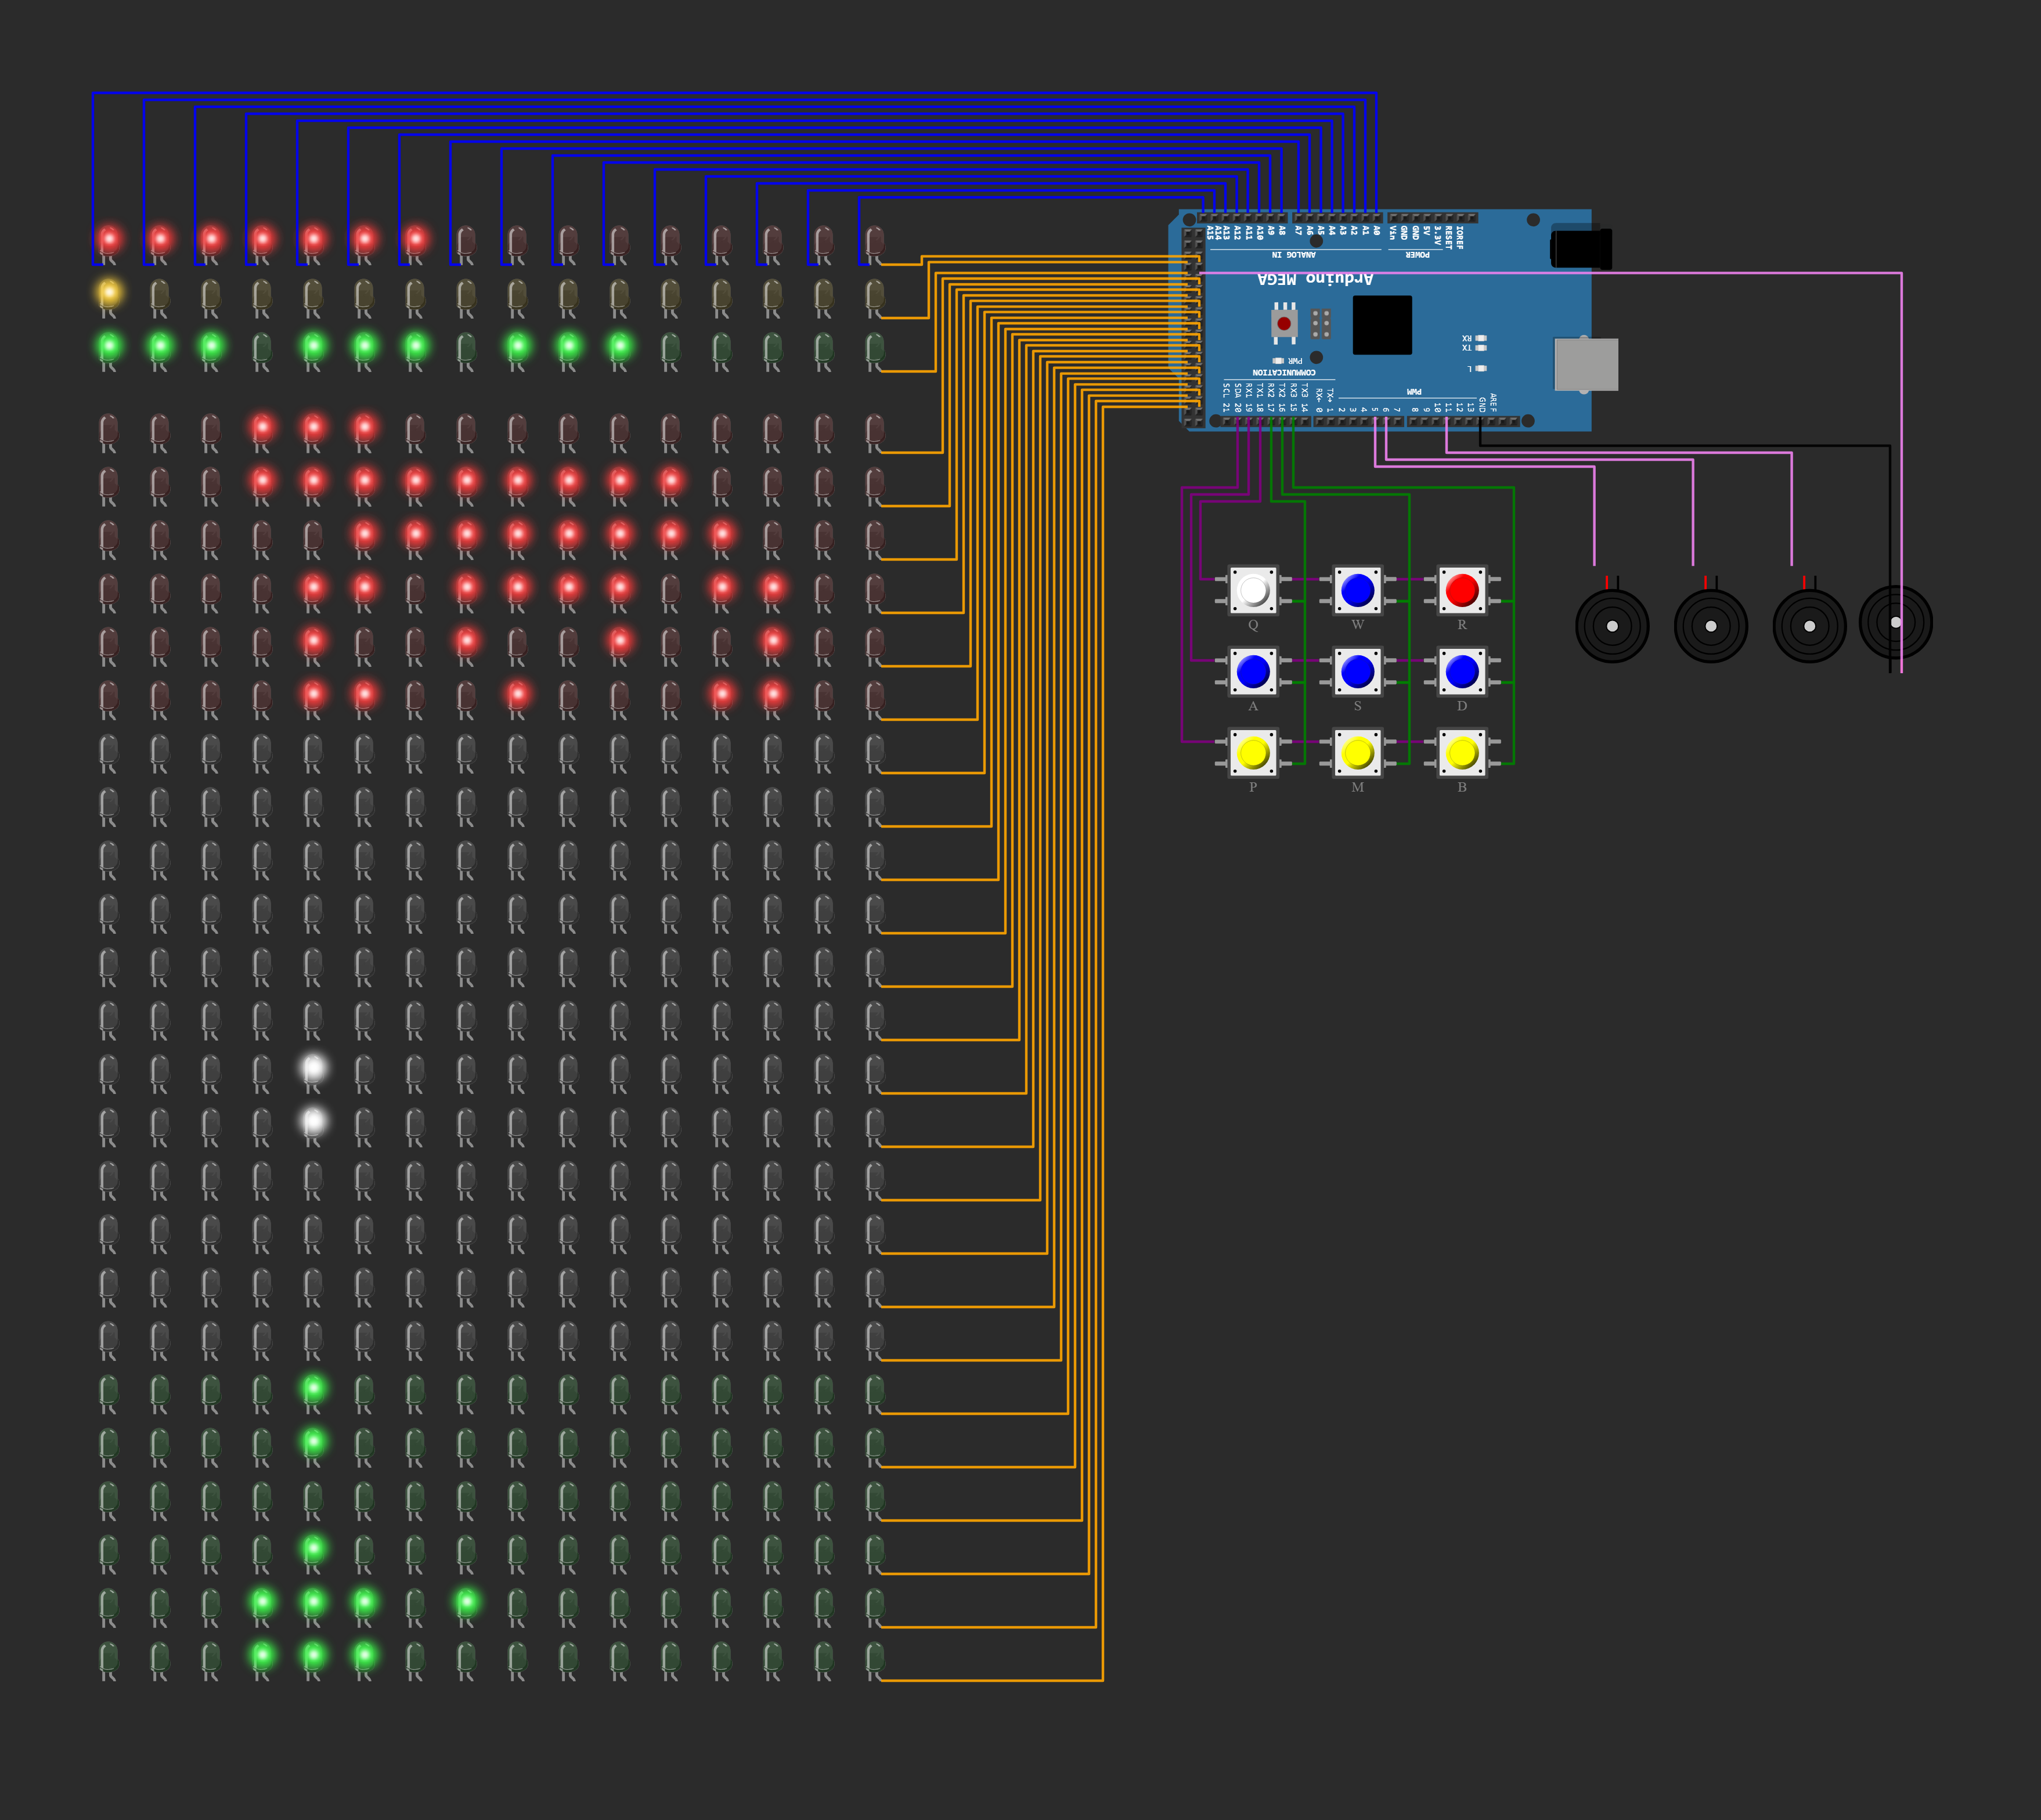
\includegraphics[width=17.00cm]{figures/circuit_photo.png}
\caption{The whole circuit in Wokwi: 432 LEDs (left), Arduino Mega 2560 (top), 3 × 3 push-button keypad and 4 buzzers (right). The LEDs show a real moment of the game: the WARDEN boss fight.}
\end{figure}

\clearpage
\section*{3. Project performance}
\phantomsection\addcontentsline{toc}{section}{3. Project performance}
\textbf{VOID RUNNER} is a complete arcade game built only from the parts the course allows: one Arduino Mega 2560, single LEDs, single push buttons and buzzers. There are no ready-made modules (no LED matrix module, no keypad module) and no libraries; the screen, the keypad and the four-voice music are all driven by our own code. The player flies a small ship at the bottom of a 16 × 24 LED screen, shoots enemies and space rocks, catches ammo crates and extra lives, and fights a boss at the end of each of the three phases. The project runs in the Wokwi simulator (Wokwi for VS Code and wokwi.com).

\subsection*{3.1 Parts and connections}
\phantomsection\addcontentsline{toc}{subsection}{3.1 Parts and connections}
\par\noindent\begin{minipage}{\linewidth}\centering\small
\begin{tabular}{|>{\raggedright\arraybackslash}p{4.78cm}|>{\raggedright\arraybackslash}p{1.43cm}|>{\raggedright\arraybackslash}p{10.04cm}|}
\hline\rowcolor{accent}\textbf{\color{white}Part} & \textbf{\color{white}Count} & \textbf{\color{white}Connection to the Mega}\\\hline
Arduino Mega 2560 & 1 & –\\\hline
\rowcolor{rowshade}Single LEDs (wokwi-led), one matrix & 432 & 16 × 24 game screen + 3 status bars of 16. 27 row wires (anodes) on pins 22–45 and 47–49, 16 column wires (cathodes) on A0–A15\\\hline
Push buttons (wokwi-pushbutton), 3 × 3 matrix & 9 & rows on pins 18–20, columns on 15–17\\\hline
\rowcolor{rowshade}Buzzers (wokwi-buzzer) & 4 & pins 5, 6, 11, 46 (outputs of Timer3, Timer4, Timer1, Timer5)\\\hline
\end{tabular}
\captionof{table}{The parts of the device.}
\end{minipage}\par\medskip

53 of the Mega's pins are used, and every header has one job: the double header drives the LED rows, the analog header the LED columns, the communication header the keypad and the PWM header the buzzers. No resistors are needed in the simulation. The circuit file (\texttt{diagram.json}) and the pin list of the code (\texttt{pins.h}) are both generated by one program (\texttt{tools/gen\_circuit.py}), which also checks every wire, so the circuit and the code always agree.

\begin{figure}[H]\centering
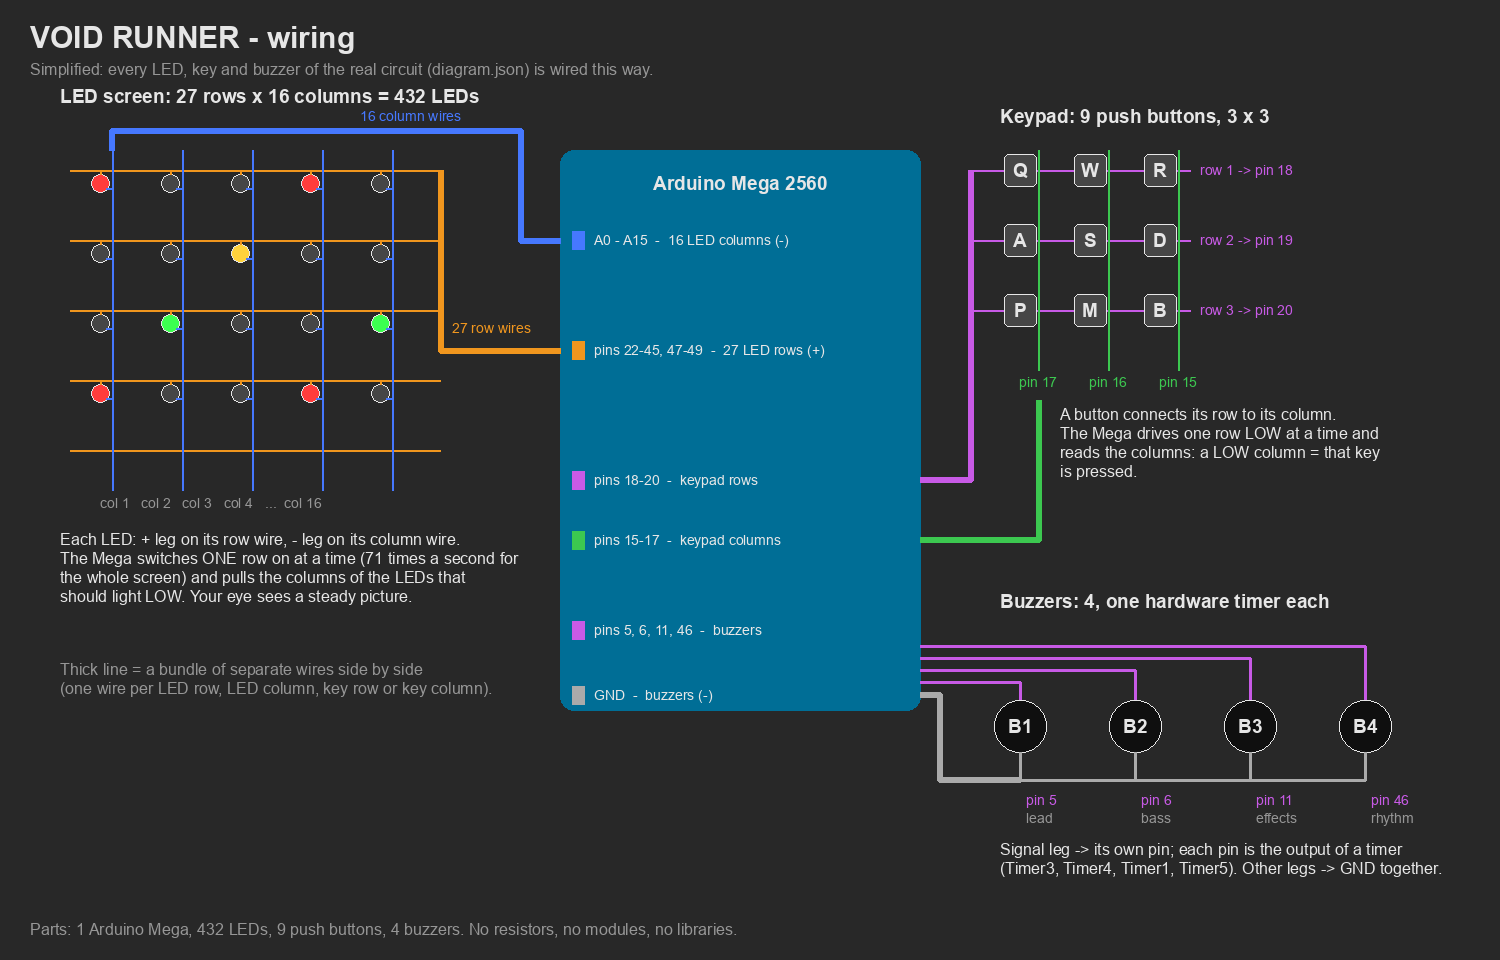
\includegraphics[width=17.00cm]{figures/wiring.png}
\caption{Simplified wiring: how every LED, key and buzzer is connected.}
\end{figure}

\subsection*{3.2 The LED screen}
\phantomsection\addcontentsline{toc}{subsection}{3.2 The LED screen}
All 432 LEDs form \textbf{one matrix} of 27 rows × 16 columns: the + leg of every LED is on its row wire, the – leg on its column wire. The Mega switches on \textbf{one row at a time} and pulls the columns of the LEDs that should light LOW. A Timer2 interrupt moves to the next row about 1900 times per second, so the whole screen is redrawn 71 times per second and the eye sees a steady picture. The columns are written with two port registers (\texttt{PORTF}, \texttt{PORTK}) at once: this costs about 3 \% of the processor, where \texttt{digitalWrite} would cost about 35 \%.

The game draws into a picture in memory (\texttt{frame}, one 16-bit word per row) and copies it to the screen when it is finished, so a half-drawn picture is never shown.

\par\noindent\begin{minipage}{\linewidth}\centering\small
\begin{tabular}{|>{\raggedright\arraybackslash}p{3.82cm}|>{\raggedright\arraybackslash}p{2.87cm}|>{\raggedright\arraybackslash}p{9.56cm}|}
\hline\rowcolor{accent}\textbf{\color{white}Area} & \textbf{\color{white}LED colour} & \textbf{\color{white}Use in the game}\\\hline
Status bar 1 & red & phase progress, then the boss's health\\\hline
\rowcolor{rowshade}Status bar 2 & yellow & ammo (blinks when low)\\\hline
Status bar 3 & green & lives (one block of 3 LEDs per life)\\\hline
\rowcolor{rowshade}Game rows 0–5 & red & where enemies and bosses enter, "WARN", "ZONE"\\\hline
Game rows 6–17 & white & open space, message pages\\\hline
\rowcolor{rowshade}Game rows 18–23 & green & the player's zone\\\hline
\end{tabular}
\captionof{table}{LED colours. Each LED has a fixed colour, like the colour strips of the 1978 Space Invaders cabinet.}
\end{minipage}\par\medskip

\begin{figure}[H]\centering
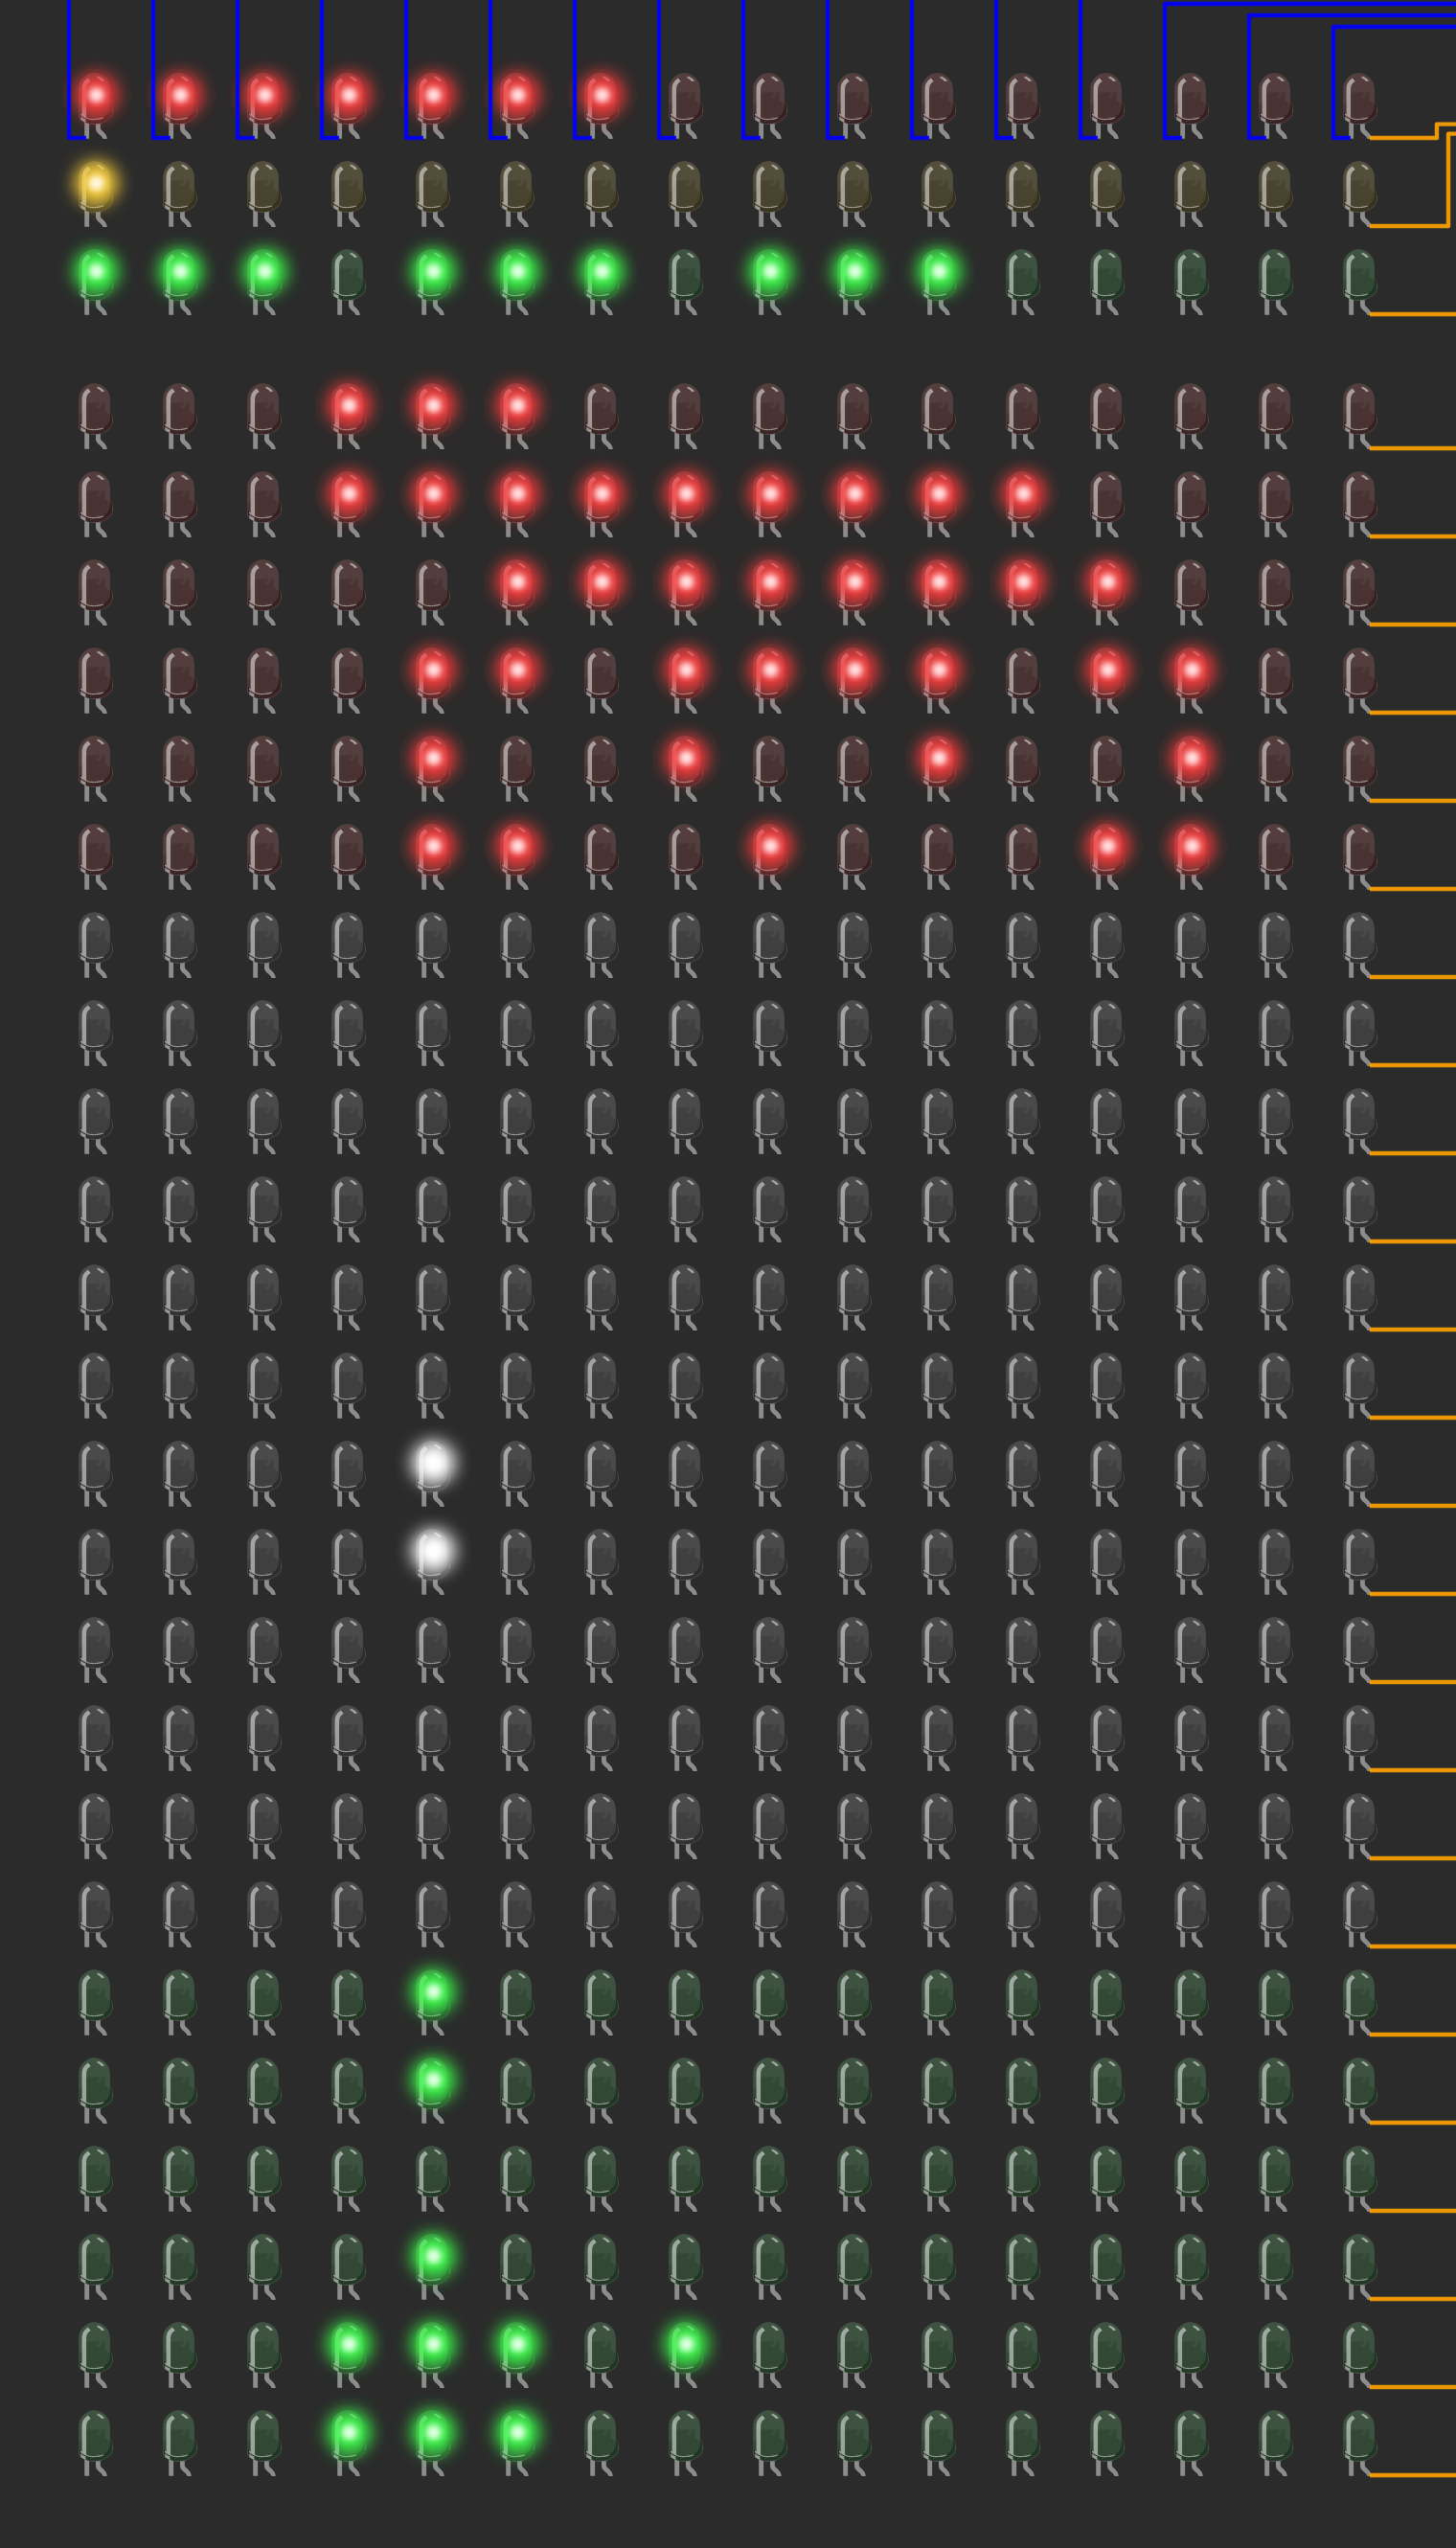
\includegraphics[width=6.50cm]{figures/cu_leds.png}
\caption{The LED panel in Wokwi during a boss fight.}
\end{figure}

\textbf{Brightness.} Each LED is lit only 1/27 of the time. Wokwi shows brightness as (share of time on)\textasciicircum{}(1/gamma); with the default gamma a lit LED looked only 32 \% bright, which was hard to see. Every LED therefore has gamma = 30 (90 \%), which is what a real multiplexed display does by driving each LED harder in its short time slot. Every LED also has fps = 300, so moving objects stay sharp, and everything that blinks stays on and off for at least 160 ms so the blink is visible.

\textbf{Text} never scrolls (scrolling letters smeared into a white block in the simulator). Every message is a still \textbf{page} of short words, at most four small letters per line, shown for 0.9 s, with big digits and signs where a word is not needed.

\subsection*{3.3 The keypad and the controls}
\phantomsection\addcontentsline{toc}{subsection}{3.3 The keypad and the controls}
The 9 push buttons form a 3 × 3 matrix, one button for each key the game uses. The code drives one row LOW at a time and reads the four columns with the internal pull-ups, so a pressed key reads LOW. The rows that are not being read are switched to inputs, so two pressed keys can never short a HIGH and a LOW output together. Every key is debounced. The buttons are labelled like keyboard keys and also react to the PC keyboard in Wokwi.

\begin{figure}[H]\centering
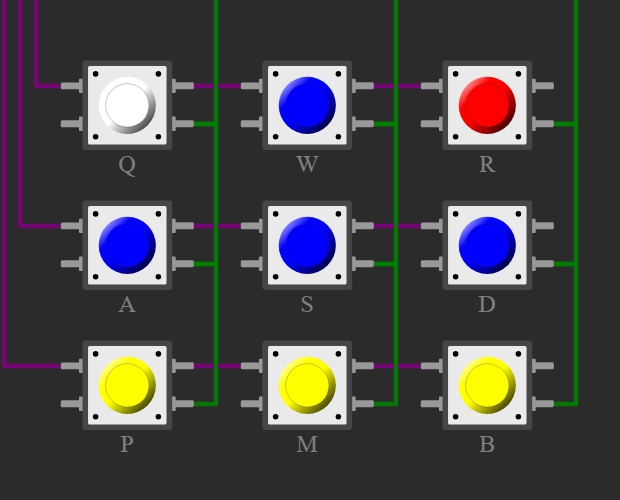
\includegraphics[width=8.00cm]{figures/cu_keypad.png}
\caption{The keypad in Wokwi.}
\end{figure}

\par\noindent\begin{minipage}{\linewidth}\centering\small
\begin{tabular}{|>{\raggedright\arraybackslash}p{2.91cm}|>{\raggedright\arraybackslash}p{13.59cm}|}
\hline\rowcolor{accent}\textbf{\color{white}Key} & \textbf{\color{white}Action}\\\hline
W A S D & move (tap = one pixel, hold = glide)\\\hline
\rowcolor{rowshade}R & fire (tap = one bullet, hold = auto-fire) · OK in the menus\\\hline
Q & back · pause in the game\\\hline
\rowcolor{rowshade}P & pause / continue\\\hline
M & sound on / off (any screen, saved)\\\hline
\rowcolor{rowshade}B & brightness 100 / 50 / 20 \% (any screen, saved)\\\hline
\end{tabular}
\captionof{table}{The keys.}
\end{minipage}\par\medskip

\textbf{Firing:} press R for one bullet; keep holding and another follows every 0.2 s (a chirp when auto-fire starts, and the ship's nose blinks). \textbf{Moving:} a tap moves one pixel, a hold makes the ship glide after 0.17 s. The newest key wins: a move key stops the fire, and while R is held the ship does not glide.

\subsection*{3.4 The four buzzers}
\phantomsection\addcontentsline{toc}{subsection}{3.4 The four buzzers}
Each buzzer is connected to the output pin of its own 16-bit hardware timer. In CTC mode with "toggle on compare match" the timer flips the pin by itself, so a note costs no processor time and \textbf{four notes can sound at once} (Arduino's \texttt{tone()} can play only one). The timers run on a slow clock (÷256), which keeps notes up to about C7 within 1 \% of their pitch.

\begin{figure}[H]\centering
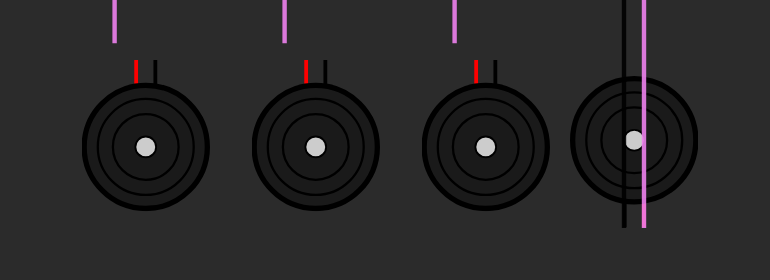
\includegraphics[width=8.00cm]{figures/cu_buzzers.png}
\caption{The four buzzers in Wokwi.}
\end{figure}

\par\noindent\begin{minipage}{\linewidth}\centering\small
\begin{tabular}{|>{\raggedright\arraybackslash}p{1.91cm}|>{\raggedright\arraybackslash}p{3.35cm}|>{\raggedright\arraybackslash}p{10.99cm}|}
\hline\rowcolor{accent}\textbf{\color{white}Buzzer} & \textbf{\color{white}Pin / timer} & \textbf{\color{white}Job}\\\hline
1 & 5 / Timer3 & lead guitar (melody)\\\hline
\rowcolor{rowshade}2 & 6 / Timer4 & bass\\\hline
3 & 11 / Timer1 & every sound effect and menu sound (music only in short jingles)\\\hline
\rowcolor{rowshade}4 & 46 / Timer5 & rhythm guitar: a fifth above the bass (bass + rhythm = a power chord)\\\hline
\end{tabular}
\captionof{table}{The voices.}
\end{minipage}\par\medskip

\subsection*{3.5 Start-up logo and welcome music}
\phantomsection\addcontentsline{toc}{subsection}{3.5 Start-up logo and welcome music}
When the device starts, a 5.6-second logo plays in sync with the welcome melody: the picture runs on the song's own clock, so every movement lands on a note. "VOID" is a vertical sign of bold 10 × 5 letters, and the status bars fill up like a start-up progress bar. Any key skips the logo.

\begin{figure}[H]\centering
\begin{minipage}[t]{2.60cm}\centering
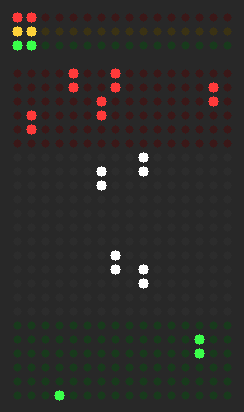
\includegraphics[width=\linewidth]{figures/logo_warp.png}\\[-2pt]
{\scriptsize\color{grey}0.6 s warp}
\end{minipage}\hspace{4pt}%
\begin{minipage}[t]{2.60cm}\centering
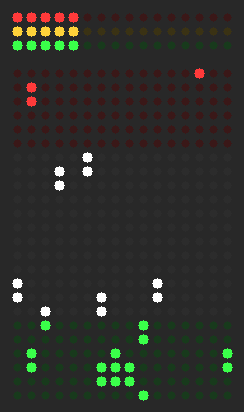
\includegraphics[width=\linewidth]{figures/logo_ship.png}\\[-2pt]
{\scriptsize\color{grey}1.6 s the ship}
\end{minipage}\hspace{4pt}%
\begin{minipage}[t]{2.60cm}\centering
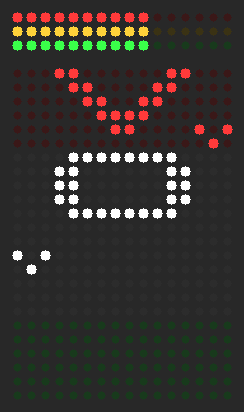
\includegraphics[width=\linewidth]{figures/logo_letters.png}\\[-2pt]
{\scriptsize\color{grey}3.1 s letters}
\end{minipage}\hspace{4pt}%
\begin{minipage}[t]{2.60cm}\centering
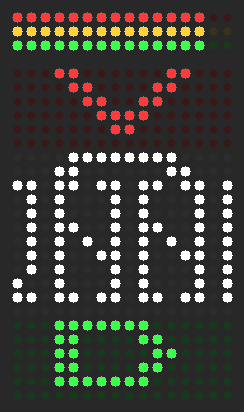
\includegraphics[width=\linewidth]{figures/logo_runner.png}\\[-2pt]
{\scriptsize\color{grey}4.2 s RUNNER}
\end{minipage}\hspace{4pt}%
\begin{minipage}[t]{2.60cm}\centering
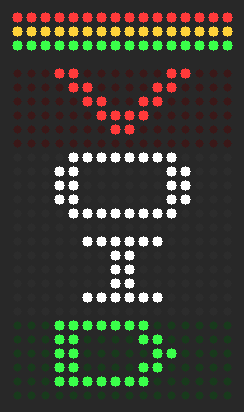
\includegraphics[width=\linewidth]{figures/logo_flash.png}\\[-2pt]
{\scriptsize\color{grey}4.9 s flash}
\end{minipage}\hspace{4pt}%
\begin{minipage}[t]{2.60cm}\centering
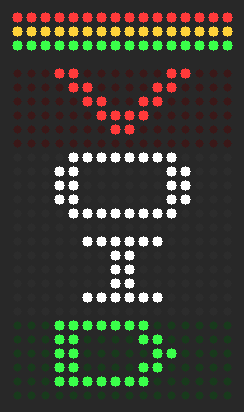
\includegraphics[width=\linewidth]{figures/logo_glow.png}\\[-2pt]
{\scriptsize\color{grey}5.4 s the sign}
\end{minipage}\hspace{4pt}%
\caption{The start-up logo.}
\end{figure}

\par\noindent\begin{minipage}{\linewidth}\centering\small
\begin{tabular}{|>{\raggedright\arraybackslash}p{2.39cm}|>{\raggedright\arraybackslash}p{7.65cm}|>{\raggedright\arraybackslash}p{6.21cm}|}
\hline\rowcolor{accent}\textbf{\color{white}Time} & \textbf{\color{white}Picture} & \textbf{\color{white}Sound}\\\hline
0.0 – 1.2 s & warp: star streaks speed up & rising whoosh + low A2 drone\\\hline
\rowcolor{rowshade}1.2 – 2.0 s & the ship rises and brakes & braking notes E4 C4 A3\\\hline
2.0 – 2.4 s & the ship shoots up and out & quick rising glide\\\hline
\rowcolor{rowshade}2.4 – 3.6 s & V, O, I, D light up one by one, flickering on; drones fly past & A4 C5 E5 A5, a crackle on each flicker\\\hline
3.6 – 4.8 s & "RUNNER" crosses on a dark ribbon, towed by the ship & melody + harmony + bass line\\\hline
\rowcolor{rowshade}4.8 – 5.6 s & the whole screen flashes, then the sign glows & A-minor chord\\\hline
\end{tabular}
\captionof{table}{Timeline of the logo.}
\end{minipage}\par\medskip

\subsection*{3.6 Title screen, demo and menu}
\phantomsection\addcontentsline{toc}{subsection}{3.6 Title screen, demo and menu}
The title screen keeps the VOID sign lit while ships fly past it, and every 7 seconds a banner shows the pages "PUSH", a big R, "TO", "PLAY". If nobody touches a key for 20 seconds a \textbf{demo} starts: the autopilot plays the game by itself until any key is pressed. R opens the menu: PLAY, SHIP, OPTS and BEST (W/S choose, R open, Q back); the chosen item is underlined.

\begin{figure}[H]\centering
\begin{minipage}[t]{3.40cm}\centering
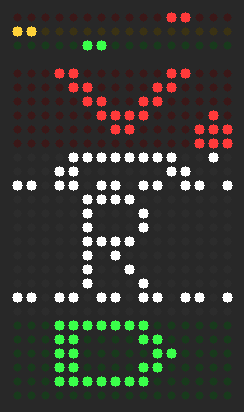
\includegraphics[width=\linewidth]{figures/title.png}\\[-2pt]
{\scriptsize\color{grey}title}
\end{minipage}\hspace{4pt}%
\begin{minipage}[t]{3.40cm}\centering
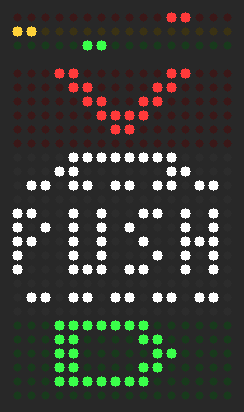
\includegraphics[width=\linewidth]{figures/title_push.png}\\[-2pt]
{\scriptsize\color{grey}banner}
\end{minipage}\hspace{4pt}%
\begin{minipage}[t]{3.40cm}\centering
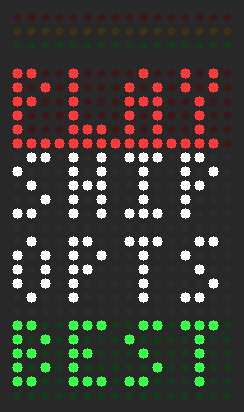
\includegraphics[width=\linewidth]{figures/menu.png}\\[-2pt]
{\scriptsize\color{grey}menu}
\end{minipage}\hspace{4pt}%
\caption{Title screen and main menu.}
\end{figure}

\subsection*{3.7 Hangar and options}
\phantomsection\addcontentsline{toc}{subsection}{3.7 Hangar and options}
In the \textbf{hangar} the player chooses one of three ships with A/D. The ship is shown three times bigger, and the three status bars show its speed, ammo and fire power. The \textbf{options} are pages: LITE (brightness), SND (sound), DIFF (EASY / NORM / HARD) and TEST (the LED test). W/S choose a page, A/D or R change it, page dots at the bottom show where you are. Every setting is saved in the EEPROM.

\begin{figure}[H]\centering
\begin{minipage}[t]{3.40cm}\centering
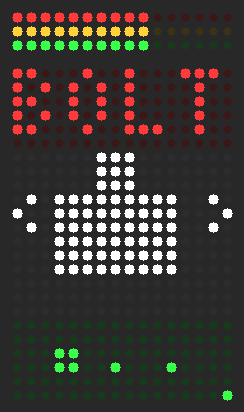
\includegraphics[width=\linewidth]{figures/hangar_bolt.png}\\[-2pt]
{\scriptsize\color{grey}BOLT}
\end{minipage}\hspace{4pt}%
\begin{minipage}[t]{3.40cm}\centering
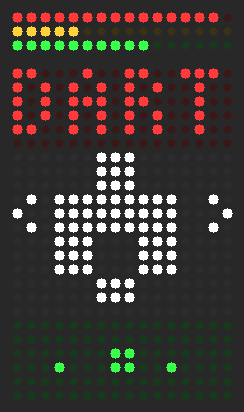
\includegraphics[width=\linewidth]{figures/hangar_dart.png}\\[-2pt]
{\scriptsize\color{grey}DART}
\end{minipage}\hspace{4pt}%
\begin{minipage}[t]{3.40cm}\centering
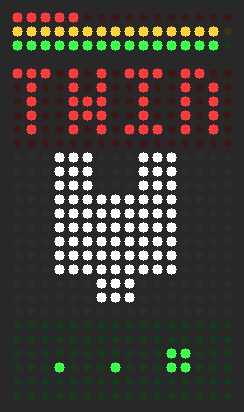
\includegraphics[width=\linewidth]{figures/hangar_twin.png}\\[-2pt]
{\scriptsize\color{grey}TWIN}
\end{minipage}\hspace{4pt}%
\caption{The hangar.}
\end{figure}

\par\noindent\begin{minipage}{\linewidth}\centering\small
\begin{tabular}{|>{\raggedright\arraybackslash}p{2.32cm}|>{\raggedright\arraybackslash}p{2.78cm}|>{\raggedright\arraybackslash}p{2.78cm}|>{\raggedright\arraybackslash}p{1.85cm}|>{\raggedright\arraybackslash}p{6.02cm}|}
\hline\rowcolor{accent}\textbf{\color{white}Ship} & \textbf{\color{white}Speed} & \textbf{\color{white}Fire} & \textbf{\color{white}Ammo} & \textbf{\color{white}Note}\\\hline
BOLT & 70 ms / pixel & every 0.20 s & 60 & balanced\\\hline
\rowcolor{rowshade}DART & 45 ms / pixel & every 0.22 s & 40 & fastest, less ammo\\\hline
TWIN & 95 ms / pixel & every 0.26 s & 80 & two bullets per shot (2 ammo), slowest\\\hline
\end{tabular}
\captionof{table}{The three ships.}
\end{minipage}\par\medskip

\begin{figure}[H]\centering
\begin{minipage}[t]{3.00cm}\centering
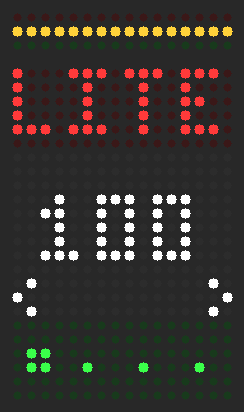
\includegraphics[width=\linewidth]{figures/opt_lite.png}\\[-2pt]
{\scriptsize\color{grey}LITE}
\end{minipage}\hspace{4pt}%
\begin{minipage}[t]{3.00cm}\centering
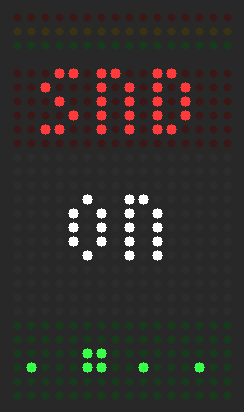
\includegraphics[width=\linewidth]{figures/opt_snd.png}\\[-2pt]
{\scriptsize\color{grey}SND}
\end{minipage}\hspace{4pt}%
\begin{minipage}[t]{3.00cm}\centering
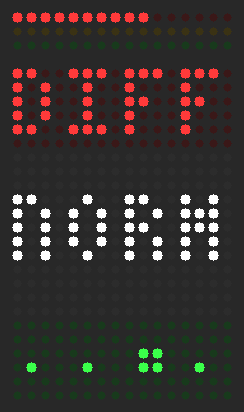
\includegraphics[width=\linewidth]{figures/opt_diff.png}\\[-2pt]
{\scriptsize\color{grey}DIFF}
\end{minipage}\hspace{4pt}%
\begin{minipage}[t]{3.00cm}\centering
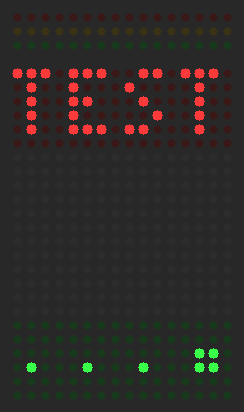
\includegraphics[width=\linewidth]{figures/opt_test.png}\\[-2pt]
{\scriptsize\color{grey}TEST}
\end{minipage}\hspace{4pt}%
\caption{The option pages.}
\end{figure}

\subsection*{3.8 Playing the game}
\phantomsection\addcontentsline{toc}{subsection}{3.8 Playing the game}
A game has three phases. Each phase starts with the pages "ZONE" and a big phase number, the phase name and "GO!" with a fanfare. Then the enemies and rocks of the phase arrive from its spawn list. When the list is finished and the screen is empty, "WARN" and a blinking warning sign appear with a siren while the red bar charges up, and the boss comes with its own music. When the boss explodes, the pages "ZONE DONE", the bonus points and "LIFE UP" follow, and the next phase begins. After the last boss the victory screen comes straight away.

\begin{figure}[H]\centering
\begin{minipage}[t]{2.60cm}\centering
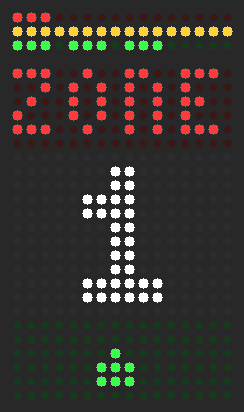
\includegraphics[width=\linewidth]{figures/zone1.png}\\[-2pt]
{\scriptsize\color{grey}ZONE 1}
\end{minipage}\hspace{4pt}%
\begin{minipage}[t]{2.60cm}\centering
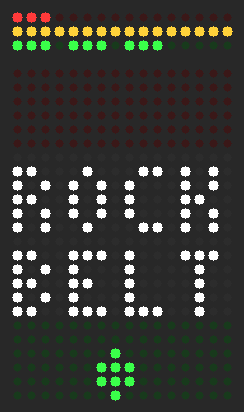
\includegraphics[width=\linewidth]{figures/rockbelt.png}\\[-2pt]
{\scriptsize\color{grey}phase name}
\end{minipage}\hspace{4pt}%
\begin{minipage}[t]{2.60cm}\centering
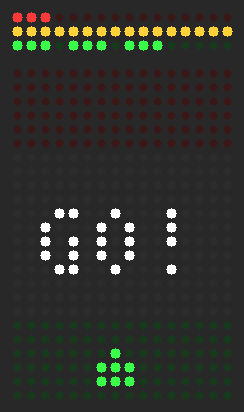
\includegraphics[width=\linewidth]{figures/go.png}\\[-2pt]
{\scriptsize\color{grey}GO!}
\end{minipage}\hspace{4pt}%
\begin{minipage}[t]{2.60cm}\centering
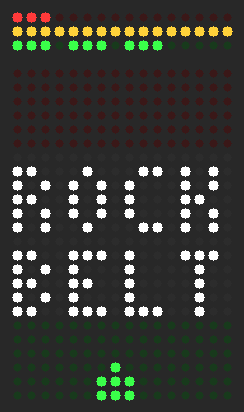
\includegraphics[width=\linewidth]{figures/phase1_0.png}\\[-2pt]
{\scriptsize\color{grey}phase 1}
\end{minipage}\hspace{4pt}%
\begin{minipage}[t]{2.60cm}\centering
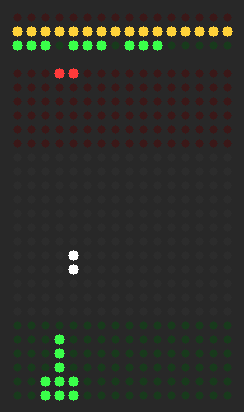
\includegraphics[width=\linewidth]{figures/phase1_1.png}\\[-2pt]
{\scriptsize\color{grey}phase 1}
\end{minipage}\hspace{4pt}%
\begin{minipage}[t]{2.60cm}\centering
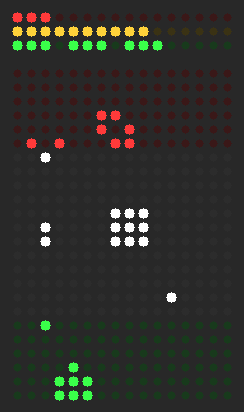
\includegraphics[width=\linewidth]{figures/phase1_3.png}\\[-2pt]
{\scriptsize\color{grey}phase 1}
\end{minipage}\hspace{4pt}%
\caption{Start of phase 1, ROCK BELT, and play.}
\end{figure}

\par\noindent\begin{minipage}{\linewidth}\centering\small
\begin{tabular}{|>{\raggedright\arraybackslash}p{2.91cm}|>{\raggedright\arraybackslash}p{13.59cm}|}
\hline\rowcolor{accent}\textbf{\color{white}Topic} & \textbf{\color{white}Rule}\\\hline
Lives & EASY 4, NORMAL 3, HARD 3 (at most 4). A hit: explosion, screen shake and 2 s of blinking shield. +1 life after each phase; extra-life pickups.\\\hline
\rowcolor{rowshade}Ammo & Per ship (60 / 40 / 80), full at the start of every phase. Ammo crates give +20 / 15 / 12 by difficulty. At 5 or less a warning beeps, the yellow bar blinks and a crate is always sent. Empty: a dry click.\\\hline
Enemies & All slower than the player; at most 4 / 5 / 6 on the screen at once (phase 1 / 2 / 3). They shoot only from the upper rows and never right next to the ship, and they never move onto each other, so the small screen stays readable.\\\hline
\rowcolor{rowshade}Space rocks & Hollow, lumpy shapes (small 3 × 3, big 4 × 3) that fall slowly and drift; a big rock takes 2 hits and breaks into two small ones. They hurt on contact.\\\hline
Explosions & Only the bosses and the player's ship explode into flying pixels; enemies just vanish with a boom (flying debris looked like bullets).\\\hline
\rowcolor{rowshade}Collisions & Pixel-exact: a hit counts only when lit pixels touch.\\\hline
Score & Drone 10, weaver 15, miner 20, cruiser 40, rocks 5 / 10, mine 2, pickup 5, bosses 200 / 300 / 500, phase bonus 100 × phase; at most 9999.\\\hline
\end{tabular}
\captionof{table}{The rules of the game.}
\end{minipage}\par\medskip

\begin{figure}[H]\centering
\begin{minipage}[t]{1.60cm}\centering

\includegraphics[width=\linewidth]{figures/sprite_enemy_drone.png}\\[-2pt]
{\scriptsize\color{grey}drone}
\end{minipage}\hspace{4pt}%
\begin{minipage}[t]{1.60cm}\centering

\includegraphics[width=\linewidth]{figures/sprite_enemy_weaver.png}\\[-2pt]
{\scriptsize\color{grey}weaver}
\end{minipage}\hspace{4pt}%
\begin{minipage}[t]{1.60cm}\centering

\includegraphics[width=\linewidth]{figures/sprite_enemy_miner.png}\\[-2pt]
{\scriptsize\color{grey}mine-layer}
\end{minipage}\hspace{4pt}%
\begin{minipage}[t]{1.60cm}\centering

\includegraphics[width=\linewidth]{figures/sprite_enemy_cruiser.png}\\[-2pt]
{\scriptsize\color{grey}cruiser}
\end{minipage}\hspace{4pt}%
\begin{minipage}[t]{1.60cm}\centering

\includegraphics[width=\linewidth]{figures/sprite_rock_small.png}\\[-2pt]
{\scriptsize\color{grey}small rock}
\end{minipage}\hspace{4pt}%
\begin{minipage}[t]{1.60cm}\centering

\includegraphics[width=\linewidth]{figures/sprite_rock_big.png}\\[-2pt]
{\scriptsize\color{grey}big rock}
\end{minipage}\hspace{4pt}%
\begin{minipage}[t]{1.60cm}\centering

\includegraphics[width=\linewidth]{figures/sprite_pickup_ammo.png}\\[-2pt]
{\scriptsize\color{grey}ammo crate}
\end{minipage}\hspace{4pt}%
\begin{minipage}[t]{1.60cm}\centering

\includegraphics[width=\linewidth]{figures/sprite_pickup_life.png}\\[-2pt]
{\scriptsize\color{grey}extra life}
\end{minipage}\hspace{4pt}%
\caption{Enemies, rocks and pickups, pixel by pixel.}
\end{figure}

\par\noindent\begin{minipage}{\linewidth}\centering\small
\begin{tabular}{|>{\raggedright\arraybackslash}p{2.91cm}|>{\raggedright\arraybackslash}p{13.59cm}|}
\hline\rowcolor{accent}\textbf{\color{white}Enemy} & \textbf{\color{white}Behaviour}\\\hline
Drone & sinks slowly, shoots straight down\\\hline
\rowcolor{rowshade}Weaver & sinks while zig-zagging, shoots now and then\\\hline
Mine-layer & crosses the top of the screen and drops mines (mines can be shot)\\\hline
\rowcolor{rowshade}Cruiser & 5 hits; stops near the top, slides sideways, fires shots aimed at the player, drops an extra life\\\hline
Rocks & fall and drift sideways; a big rock breaks into two\\\hline
\end{tabular}
\captionof{table}{Enemy types.}
\end{minipage}\par\medskip

\subsection*{3.9 The status bars}
\phantomsection\addcontentsline{toc}{subsection}{3.9 The status bars}
The three bars above the game screen show the state of the game at a glance. Red: how far the phase has come; during the warning it charges up, and in the boss fight it shows the boss's health, dropping with every hit. Yellow: the ammo left (it blinks when 5 or fewer are left). Green: the lives, one block of three LEDs per life.

\subsection*{3.10 The three phases and their bosses}
\phantomsection\addcontentsline{toc}{subsection}{3.10 The three phases and their bosses}
\par\noindent\begin{minipage}{\linewidth}\centering\small
\begin{tabular}{|>{\raggedright\arraybackslash}p{2.87cm}|>{\raggedright\arraybackslash}p{4.30cm}|>{\raggedright\arraybackslash}p{9.08cm}|}
\hline\rowcolor{accent}\textbf{\color{white}Phase} & \textbf{\color{white}Enemies} & \textbf{\color{white}Boss}\\\hline
1 – ROCK BELT & drones and many rocks & \textbf{WARDEN}: wide (10 × 4), slides along the top, 3-way spread, drops rocks; below half health faster with a 5-way spread\\\hline
\rowcolor{rowshade}2 – DEEP MIST & weavers, mine-layers, drones & \textbf{HUNTER}: small and fast; dashes to a new spot, fires an aimed pair, and every 7 s blinks and dives at the player\\\hline
3 – THE VOID & cruisers, everything else, rock showers & \textbf{VOID KING}: huge (12 × 5), 5-way spread, calls in drones; at half health its eye opens (roar, shake), then aimed triple volleys and rock rain\\\hline
\end{tabular}
\captionof{table}{Phases and bosses. Boss health: 24 / 22 / 40, scaled by the difficulty.}
\end{minipage}\par\medskip

\begin{figure}[H]\centering
\begin{minipage}[t]{2.60cm}\centering
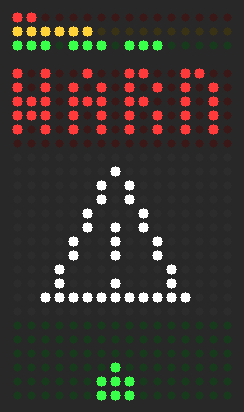
\includegraphics[width=\linewidth]{figures/warn1.png}\\[-2pt]
{\scriptsize\color{grey}WARN}
\end{minipage}\hspace{4pt}%
\begin{minipage}[t]{2.60cm}\centering
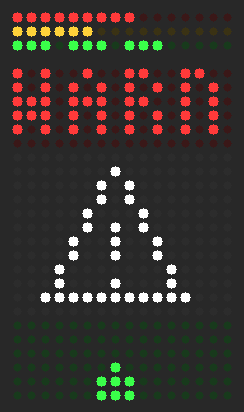
\includegraphics[width=\linewidth]{figures/warn2.png}\\[-2pt]
{\scriptsize\color{grey}warning sign}
\end{minipage}\hspace{4pt}%
\begin{minipage}[t]{2.60cm}\centering
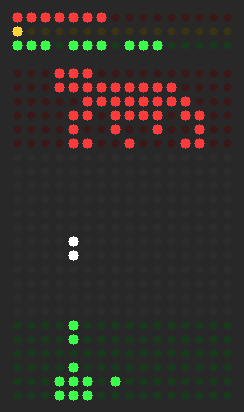
\includegraphics[width=\linewidth]{figures/warden_0.png}\\[-2pt]
{\scriptsize\color{grey}WARDEN}
\end{minipage}\hspace{4pt}%
\begin{minipage}[t]{2.60cm}\centering
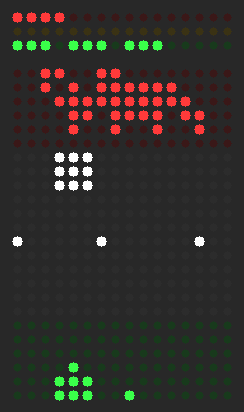
\includegraphics[width=\linewidth]{figures/warden_1.png}\\[-2pt]
{\scriptsize\color{grey}WARDEN}
\end{minipage}\hspace{4pt}%
\begin{minipage}[t]{2.60cm}\centering
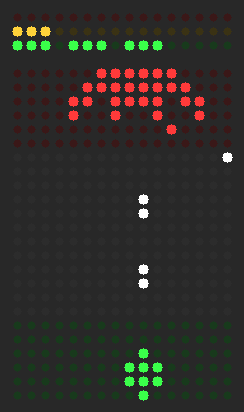
\includegraphics[width=\linewidth]{figures/bossdown.png}\\[-2pt]
{\scriptsize\color{grey}boss down}
\end{minipage}\hspace{4pt}%
\begin{minipage}[t]{2.60cm}\centering
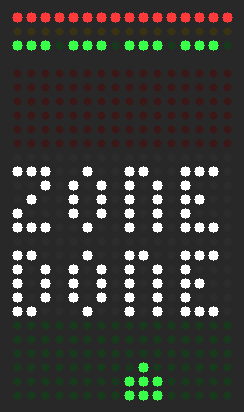
\includegraphics[width=\linewidth]{figures/zonedone.png}\\[-2pt]
{\scriptsize\color{grey}ZONE DONE}
\end{minipage}\hspace{4pt}%
\caption{Phase 1: the warning, the WARDEN fight and the end of the phase.}
\end{figure}

\begin{figure}[H]\centering
\begin{minipage}[t]{2.60cm}\centering
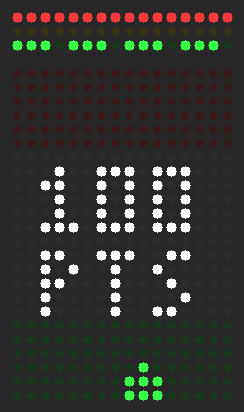
\includegraphics[width=\linewidth]{figures/pts.png}\\[-2pt]
{\scriptsize\color{grey}bonus}
\end{minipage}\hspace{4pt}%
\begin{minipage}[t]{2.60cm}\centering
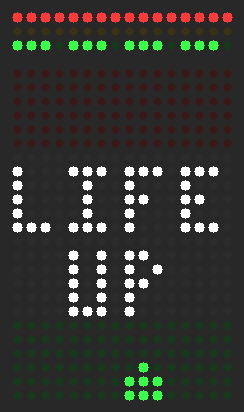
\includegraphics[width=\linewidth]{figures/lifeup.png}\\[-2pt]
{\scriptsize\color{grey}LIFE UP}
\end{minipage}\hspace{4pt}%
\begin{minipage}[t]{2.60cm}\centering
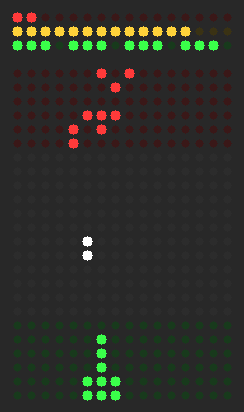
\includegraphics[width=\linewidth]{figures/phase2a.png}\\[-2pt]
{\scriptsize\color{grey}phase 2}
\end{minipage}\hspace{4pt}%
\begin{minipage}[t]{2.60cm}\centering
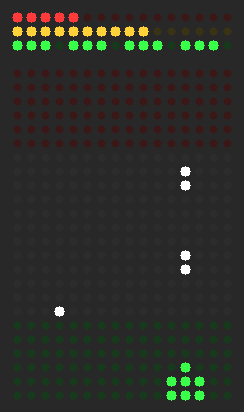
\includegraphics[width=\linewidth]{figures/phase2b.png}\\[-2pt]
{\scriptsize\color{grey}phase 2}
\end{minipage}\hspace{4pt}%
\begin{minipage}[t]{2.60cm}\centering
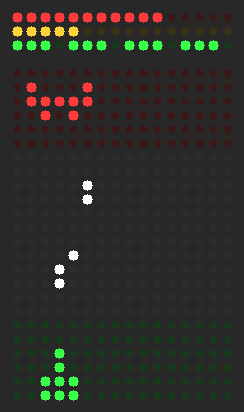
\includegraphics[width=\linewidth]{figures/hunter1.png}\\[-2pt]
{\scriptsize\color{grey}HUNTER}
\end{minipage}\hspace{4pt}%
\begin{minipage}[t]{2.60cm}\centering
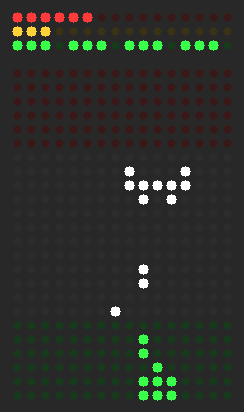
\includegraphics[width=\linewidth]{figures/hunter2.png}\\[-2pt]
{\scriptsize\color{grey}HUNTER}
\end{minipage}\hspace{4pt}%
\caption{Phase 2, DEEP MIST, and the HUNTER.}
\end{figure}

\begin{figure}[H]\centering
\begin{minipage}[t]{2.60cm}\centering
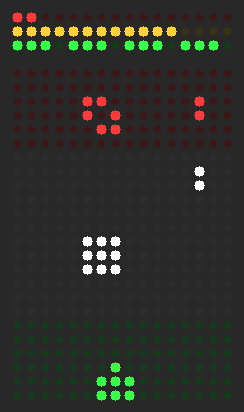
\includegraphics[width=\linewidth]{figures/phase3a.png}\\[-2pt]
{\scriptsize\color{grey}phase 3}
\end{minipage}\hspace{4pt}%
\begin{minipage}[t]{2.60cm}\centering
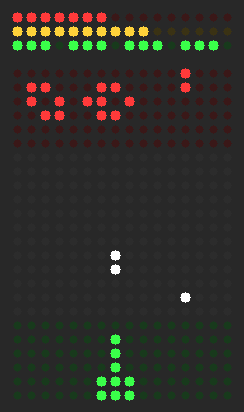
\includegraphics[width=\linewidth]{figures/phase3b.png}\\[-2pt]
{\scriptsize\color{grey}phase 3}
\end{minipage}\hspace{4pt}%
\begin{minipage}[t]{2.60cm}\centering
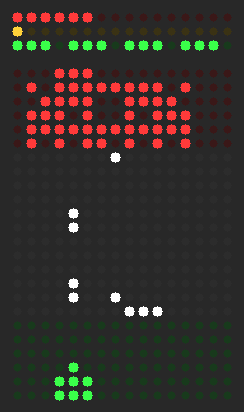
\includegraphics[width=\linewidth]{figures/king_0.png}\\[-2pt]
{\scriptsize\color{grey}VOID KING}
\end{minipage}\hspace{4pt}%
\begin{minipage}[t]{2.60cm}\centering
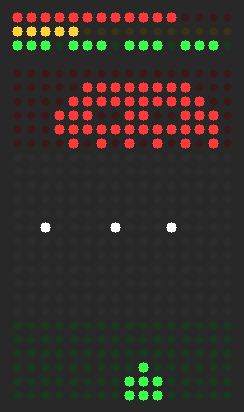
\includegraphics[width=\linewidth]{figures/king.png}\\[-2pt]
{\scriptsize\color{grey}VOID KING}
\end{minipage}\hspace{4pt}%
\begin{minipage}[t]{2.60cm}\centering
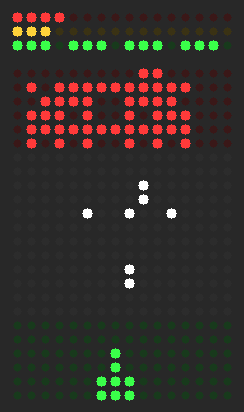
\includegraphics[width=\linewidth]{figures/king_2.png}\\[-2pt]
{\scriptsize\color{grey}eye open}
\end{minipage}\hspace{4pt}%
\begin{minipage}[t]{2.60cm}\centering
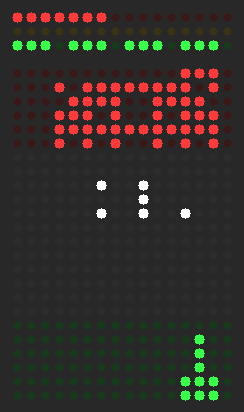
\includegraphics[width=\linewidth]{figures/king2.png}\\[-2pt]
{\scriptsize\color{grey}form 2}
\end{minipage}\hspace{4pt}%
\caption{Phase 3, THE VOID, and the VOID KING in both forms.}
\end{figure}

\begin{figure}[H]\centering
\begin{minipage}[t]{3.50cm}\centering

\includegraphics[width=\linewidth]{figures/sprite_boss_warden.png}\\[-2pt]
{\scriptsize\color{grey}WARDEN}
\end{minipage}\hspace{4pt}%
\begin{minipage}[t]{3.50cm}\centering

\includegraphics[width=\linewidth]{figures/sprite_boss_hunter.png}\\[-2pt]
{\scriptsize\color{grey}HUNTER}
\end{minipage}\hspace{4pt}%
\begin{minipage}[t]{3.50cm}\centering

\includegraphics[width=\linewidth]{figures/sprite_boss_king.png}\\[-2pt]
{\scriptsize\color{grey}VOID KING}
\end{minipage}\hspace{4pt}%
\begin{minipage}[t]{3.50cm}\centering

\includegraphics[width=\linewidth]{figures/sprite_boss_king_angry.png}\\[-2pt]
{\scriptsize\color{grey}VOID KING, form 2}
\end{minipage}\hspace{4pt}%
\caption{The bosses, pixel by pixel.}
\end{figure}

\par\noindent\begin{minipage}{\linewidth}\centering\small
\begin{tabular}{|>{\raggedright\arraybackslash}p{3.05cm}|>{\raggedright\arraybackslash}p{2.03cm}|>{\raggedright\arraybackslash}p{4.06cm}|>{\raggedright\arraybackslash}p{3.56cm}|>{\raggedright\arraybackslash}p{3.05cm}|}
\hline\rowcolor{accent}\textbf{\color{white}Difficulty} & \textbf{\color{white}Lives} & \textbf{\color{white}Enemy fire} & \textbf{\color{white}Boss health} & \textbf{\color{white}Ammo crate}\\\hline
EASY & 4 & 1.5 × slower & 80 \% & +20\\\hline
\rowcolor{rowshade}NORMAL & 3 & normal & 100 \% & +15\\\hline
HARD & 3 & 1.33 × faster & 130 \% & +12\\\hline
\end{tabular}
\captionof{table}{Difficulty levels (OPTS → DIFF).}
\end{minipage}\par\medskip

\subsection*{3.11 Pause, game over, victory and best score}
\phantomsection\addcontentsline{toc}{subsection}{3.11 Pause, game over, victory and best score}
\textbf{P} (or Q) pauses the game: the game clock stops, the score and a big pause sign are shown, and the pages "P:GO" / "Q:EX" explain the keys. When the last life is lost, \textbf{GAME OVER} shows the score (blinking for a new record) and the best score. After the VOID KING the \textbf{victory} screen shows fireworks and the pages "YOU WIN!", "VOID SAFE" and the score. The \textbf{BEST} page shows the high score, how far that game got (ZONE 1–3, or WIN) and its difficulty; it is kept in the EEPROM, so it survives a power cut on a real Arduino.

\begin{figure}[H]\centering
\begin{minipage}[t]{2.90cm}\centering
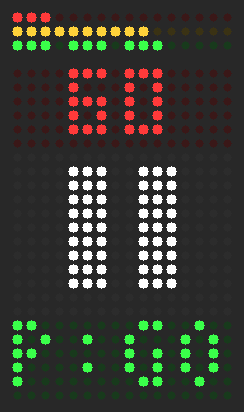
\includegraphics[width=\linewidth]{figures/pause_score.png}\\[-2pt]
{\scriptsize\color{grey}pause}
\end{minipage}\hspace{4pt}%
\begin{minipage}[t]{2.90cm}\centering
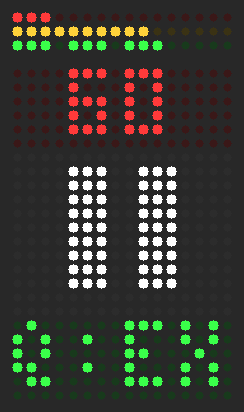
\includegraphics[width=\linewidth]{figures/pause_sign.png}\\[-2pt]
{\scriptsize\color{grey}pause}
\end{minipage}\hspace{4pt}%
\begin{minipage}[t]{2.90cm}\centering
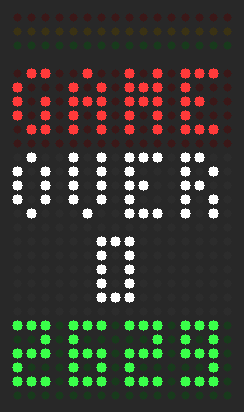
\includegraphics[width=\linewidth]{figures/over1.png}\\[-2pt]
{\scriptsize\color{grey}game over}
\end{minipage}\hspace{4pt}%
\begin{minipage}[t]{2.90cm}\centering
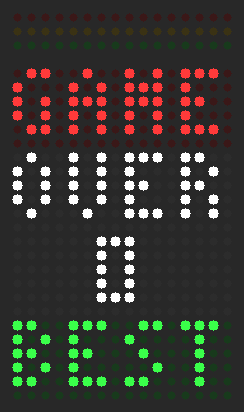
\includegraphics[width=\linewidth]{figures/over2.png}\\[-2pt]
{\scriptsize\color{grey}game over}
\end{minipage}\hspace{4pt}%
\begin{minipage}[t]{2.90cm}\centering
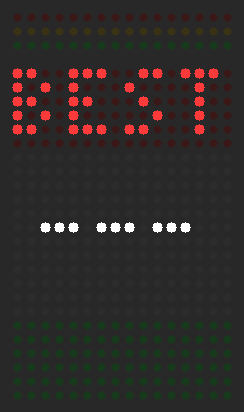
\includegraphics[width=\linewidth]{figures/best_empty.png}\\[-2pt]
{\scriptsize\color{grey}no record yet}
\end{minipage}\hspace{4pt}%
\caption{Pause and game over.}
\end{figure}

\begin{figure}[H]\centering
\begin{minipage}[t]{2.60cm}\centering
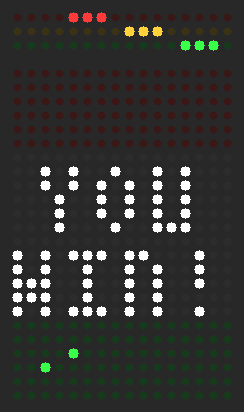
\includegraphics[width=\linewidth]{figures/vic_d.png}\\[-2pt]
{\scriptsize\color{grey}YOU WIN!}
\end{minipage}\hspace{4pt}%
\begin{minipage}[t]{2.60cm}\centering
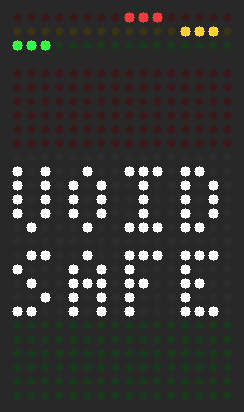
\includegraphics[width=\linewidth]{figures/vic_a.png}\\[-2pt]
{\scriptsize\color{grey}VOID SAFE}
\end{minipage}\hspace{4pt}%
\begin{minipage}[t]{2.60cm}\centering
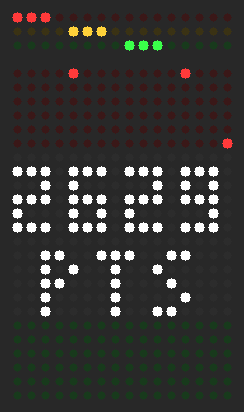
\includegraphics[width=\linewidth]{figures/vic_c.png}\\[-2pt]
{\scriptsize\color{grey}score}
\end{minipage}\hspace{4pt}%
\begin{minipage}[t]{2.60cm}\centering
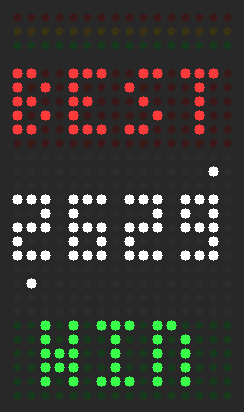
\includegraphics[width=\linewidth]{figures/best1.png}\\[-2pt]
{\scriptsize\color{grey}BEST}
\end{minipage}\hspace{4pt}%
\begin{minipage}[t]{2.60cm}\centering
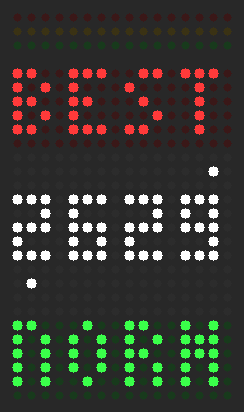
\includegraphics[width=\linewidth]{figures/best2.png}\\[-2pt]
{\scriptsize\color{grey}how far}
\end{minipage}\hspace{4pt}%
\begin{minipage}[t]{2.60cm}\centering
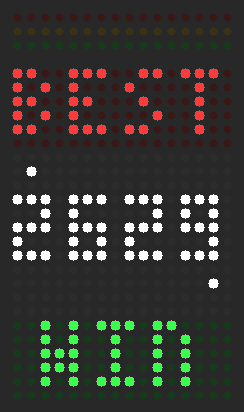
\includegraphics[width=\linewidth]{figures/best3.png}\\[-2pt]
{\scriptsize\color{grey}difficulty}
\end{minipage}\hspace{4pt}%
\caption{Victory and the best score.}
\end{figure}

\subsection*{3.12 Sound and music}
\phantomsection\addcontentsline{toc}{subsection}{3.12 Sound and music}
All music is written as note lists, one per buzzer, stored in flash. The in-game songs are original metal tracks written for this project in a short notation (\texttt{tools/compose\_music.py}): buzzer 1 plays the lead guitar, buzzer 2 the bass and buzzer 4 a rhythm guitar a fifth above the bass, which together sound like a power chord. Buzzer 3 is kept free for sound effects, so an effect never cuts the music.

\par\noindent\begin{minipage}{\linewidth}\centering\small
\begin{tabular}{|>{\raggedright\arraybackslash}p{3.82cm}|>{\raggedright\arraybackslash}p{5.74cm}|>{\raggedright\arraybackslash}p{6.69cm}|}
\hline\rowcolor{accent}\textbf{\color{white}Song} & \textbf{\color{white}Style} & \textbf{\color{white}Character}\\\hline
ROCK BELT (phase 1) & fast thrash, E minor, about 190 BPM, loop 10.2 s & the gallop rhythm on low E; a question-and-answer melody\\\hline
\rowcolor{rowshade}DEEP MIST (phase 2) & slow and heavy, drop-D, half-time, loop 12.8 s & short muted chugs with gaps; sparse, spooky lead\\\hline
THE VOID (phase 3) & syncopated groove, E minor, loop 9.6 s & off-beat stabs; a hook you can hum\\\hline
\rowcolor{rowshade}Boss (all three) & tremolo picking, chromatic, about 210 BPM, loop 4.5 s & nonstop 16th notes; a wailing lead figure\\\hline
\end{tabular}
\captionof{table}{The in-game songs.}
\end{minipage}\par\medskip

Other music: the start-up melody, the phase fanfare, phase clear, victory and game over. Sound effects use priorities, so an important sound is never cut by a small one: shot, auto-fire chirp, empty click, hit, explosion, big explosion, player hit, pickup, extra life, low ammo, warning siren, boss roar and the LED-test sweep. Explosions are noise (a random frequency every 6 ms); the other effects slide between two frequencies.

\subsection*{3.13 LED test}
\phantomsection\addcontentsline{toc}{subsection}{3.13 LED test}
OPTS → TEST checks the hardware: every LED on, then a row sweep (status bars first), a column sweep and a checkerboard, with rising beeps. A broken LED or wire is easy to spot.

\begin{figure}[H]\centering
\begin{minipage}[t]{3.00cm}\centering
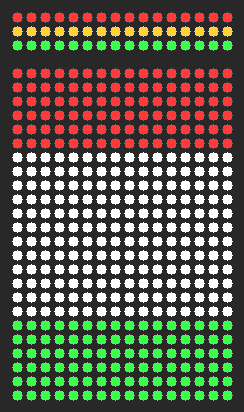
\includegraphics[width=\linewidth]{figures/led1.png}\\[-2pt]
{\scriptsize\color{grey}all on}
\end{minipage}\hspace{4pt}%
\begin{minipage}[t]{3.00cm}\centering

\includegraphics[width=\linewidth]{figures/led2.png}\\[-2pt]
{\scriptsize\color{grey}rows}
\end{minipage}\hspace{4pt}%
\begin{minipage}[t]{3.00cm}\centering
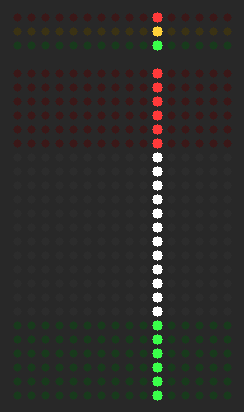
\includegraphics[width=\linewidth]{figures/led3.png}\\[-2pt]
{\scriptsize\color{grey}columns}
\end{minipage}\hspace{4pt}%
\begin{minipage}[t]{3.00cm}\centering
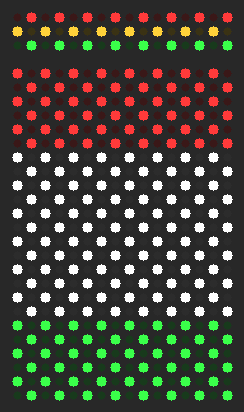
\includegraphics[width=\linewidth]{figures/led4.png}\\[-2pt]
{\scriptsize\color{grey}checkerboard}
\end{minipage}\hspace{4pt}%
\caption{The LED test.}
\end{figure}

\subsection*{3.14 Reliability and measurements}
\phantomsection\addcontentsline{toc}{subsection}{3.14 Reliability and measurements}
\begin{itemize}
  \item \textbf{Nothing blocks:} there is no \texttt{delay()} in the game. A new picture is made every 20 ms, and each part of the program does one small step per picture. The game has its own clock (\texttt{gameMs}) that stops while paused.
  \item \textbf{Screen:} the Timer2 interrupt shows the picture whatever the game code is doing; 3 \% of the processor.
  \item \textbf{Simulation speed:} the timers run on slow clocks and unused timers are stopped, because Wokwi spends time on every timer count. Measured: about 93 \% of real time during the logo and 91 \% with every LED lit.
  \item \textbf{Memory:} only fixed-size arrays (no \texttt{malloc}), so nothing can run out during a game. 33 KB of 248 KB flash and 2.0 KB of 8 KB RAM are used; fonts, pixel art, music and spawn lists are kept in flash.
  \item \textbf{Fairness:} at most 4–6 enemies at once, no shots from close range, a crate always comes when the ammo runs low, and every phase was checked to be winnable.
\end{itemize}

\subsection*{3.15 Testing}
\phantomsection\addcontentsline{toc}{subsection}{3.15 Testing}
Besides playing it in Wokwi, the real game code is compiled on the PC together with a small stand-in for the Arduino (registers as variables, a simulated clock, a simulated keypad). Test scripts press keys and check the Serial output and the screen, so a whole game runs in under a second. An \textbf{autopilot} that plays like a careful player was used to check that every phase can be won, and to tune the difficulty.

\par\noindent\begin{minipage}{\linewidth}\centering\small
\begin{tabular}{|>{\raggedright\arraybackslash}p{2.39cm}|>{\raggedright\arraybackslash}p{9.56cm}|>{\raggedright\arraybackslash}p{4.30cm}|}
\hline\rowcolor{accent}\textbf{\color{white}Test} & \textbf{\color{white}What it checks} & \textbf{\color{white}Result}\\\hline
controls & tap, glide, row limit, single shot, auto-fire rate, move cancels fire, no glide while firing & pass\\\hline
\rowcolor{rowshade}screens & logo skip, title, menu, hangar, options, LED test, best, pause, game over and new record, global keys, power cycle (EEPROM), demo & pass\\\hline
playthrough & all three phases and bosses, VOID KING form 2, victory & pass\\\hline
\rowcolor{rowshade}balance & autopilot without shield, reacting only every 250 ms (roughly a human), 48 games per difficulty & EASY 47/48, NORMAL 38/48, HARD 27/48 won\\\hline
QA run & four test agents played and stress-tested every part (1000+ games and random key runs) & no crash or hang; findings fixed or listed\\\hline
\end{tabular}
\captionof{table}{Automatic tests.}
\end{minipage}\par\medskip

Serial test commands (typed in the Wokwi terminal, starting with \texttt{!}) help with testing: \texttt{!d} shows the screen as text, \texttt{!s} the game state, \texttt{!1}–\texttt{!3} start at a phase, \texttt{!b} skips to the boss, \texttt{!i} gives a shield and \texttt{!x} turns on the autopilot.

\clearpage
\section*{4. Project code}
\phantomsection\addcontentsline{toc}{section}{4. Project code}
The program is written in C++ for the Arduino Mega (Arduino core functions plus direct register access where speed or timing needs it; no libraries). It is one sketch, \texttt{void\_runner.ino}, with one header file per module; in Wokwi every file is a tab. All files together are compiled as one unit. The game logic advances in steps of 20 ms; the screen and the sound run on hardware timers.

{\small\begin{longtable}{|>{\raggedright\arraybackslash}p{4.30cm}|>{\raggedright\arraybackslash}p{10.04cm}|>{\raggedright\arraybackslash}p{1.91cm}|}
\hline\rowcolor{accent}\textbf{\color{white}File} & \textbf{\color{white}Contents} & \textbf{\color{white}Lines}\\\hline\endhead
void\_runner.ino & The main file & 283\\\hline
\rowcolor{rowshade}config.h & Settings & 43\\\hline
pins.h & Pin numbers (generated) & 39\\\hline
\rowcolor{rowshade}display.h & The LED screen & 243\\\hline
input.h & The keypad & 74\\\hline
\rowcolor{rowshade}sound.h & The sound engine & 244\\\hline
tunes.h & Songs and sound effects & 201\\\hline
\rowcolor{rowshade}storage.h & EEPROM: settings and best score & 64\\\hline
font.h & Fonts (generated) & 99\\\hline
\rowcolor{rowshade}art.h & Pixel art & 147\\\hline
logo.h & Start-up logo and welcome melody & 161\\\hline
\rowcolor{rowshade}title.h & Title screen & 34\\\hline
menu.h & Main menu & 53\\\hline
\rowcolor{rowshade}world.h & Everything on the game screen & 268\\\hline
player.h & The player's ship & 143\\\hline
\rowcolor{rowshade}enemies.h & Enemies and rocks & 167\\\hline
levels.h & The three phases & 89\\\hline
\rowcolor{rowshade}boss.h & The bosses & 200\\\hline
game.h & One game & 536\\\hline
\rowcolor{rowshade}autopilot.h & Autopilot & 143\\\hline
screens.h & The other screens & 319\\\hline
\rowcolor{rowshade}\textbf{total} &  & \textbf{3550}\\\hline
\caption{The files of the program.}\\
\end{longtable}}

Each file below starts with a short explanation and the list of its functions (taken from the description written above every function), followed by the full source code.

\clearpage
\subsection*{4.1 void\_runner.ino – The main file}
\phantomsection\addcontentsline{toc}{subsection}{4.1 void\_runner.ino – The main file}
The sketch that Wokwi compiles; every other file is a tab of it (one translation unit). \texttt{setup()} stops the unused timers, starts the screen, the keypad and the sound, and loads the saved settings. \texttt{loop()} makes one picture every 20 ms: it reads the keys, handles the global keys M and B, runs the current screen and plays the sound. The screens form a state machine (logo → title → menu → game → pause / game over / victory …): each screen function returns the screen to show next. The Serial test commands (\texttt{!d}, \texttt{!s}, …) are handled here too.

\begin{figure}[H]\centering
\begin{minipage}[t]{3.60cm}\centering
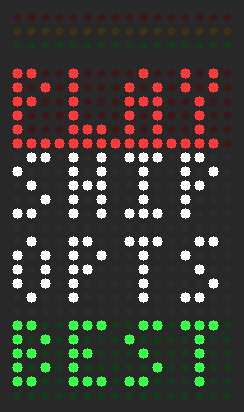
\includegraphics[width=\linewidth]{figures/menu.png}\\[-2pt]
{\scriptsize\color{grey}}
\end{minipage}\hspace{4pt}%
\caption{What void\_runner.ino draws or uses.}
\end{figure}

\par\noindent\begin{minipage}{\linewidth}\centering\footnotesize
\begin{tabular}{|>{\raggedright\arraybackslash}p{5.82cm}|>{\raggedright\arraybackslash}p{10.68cm}|}
\hline\rowcolor{accent}\textbf{\color{white}Function} & \textbf{\color{white}What it does}\\\hline
goTo(Screen next) & Switches to another screen: remembers when it opened, logs it, and does what that screen needs first (start the logo music, stop sounds, save the score, ...).\\\hline
\rowcolor{rowshade}globalKeys() & Keys that work on every screen: B = brightness, M = sound on/off (both saved).\\\hline
serialCommands() & Test commands over Serial start with '!', so letters typed by mistake into the Wokwi terminal do nothing (they usually mean the keyboard is talking to the terminal instead of the buttons): !d  print the screen as text      !s  print the game state !1 !2 !3  start a game at phase 1, 2 or 3 !b  skip to the boss              !w  the boss loses all its health !i  shield on/off (no hits)       !x  autopilot on/off !f  fast mode on/off (8 game steps per picture) !k  lose the last life\\\hline
\rowcolor{rowshade}drawScreen(uint32\_t now) & One picture of the current screen: handles its keys, draws it and switches to another screen when needed (the screen state machine).\\\hline
setup() & Runs once at power-on: Serial, LED screen, keypad, buzzers and the saved settings, then the start-up logo.\\\hline
\rowcolor{rowshade}loop() & Runs over and over: reads the keypad, keeps the music going, reads test commands, and every 20 ms draws a new picture.\\\hline
\end{tabular}
\end{minipage}\par\medskip

\subsubsection*{Source code}
\phantomsection\addcontentsline{toc}{subsubsection}{Source code}
\begin{lstlisting}[language=Arduino]
/*
 * VOID RUNNER -- a vertical space shooter on an Arduino Mega.
 *
 * Hardware (see diagram.json; pins.h is generated with it by tools/gen_circuit.py):
 *   - 16 x 24 game screen + 3 status bars, 432 single LEDs in one row/column matrix
 *   - 3 x 3 keypad of single push buttons (W A S D move, R fire / OK, Q back,
 *     P pause, M sound on/off, B brightness)
 *   - 4 buzzers, one hardware timer each: lead, bass, effects, rhythm guitar
 *
 * Code tabs:
 *   config.h   settings              display.h  LED screen, drawing, text
 *   input.h    keypad                sound.h    buzzers, music engine, effects
 *   tunes.h    songs and effects     storage.h  settings + high score in EEPROM
 *   art.h      pixel art             font.h     two pixel fonts (generated)
 *   logo.h     start-up logo         title.h    title screen
 *   menu.h     main menu             screens.h  hangar, options, best, pause, end screens
 *   world.h    everything on the game screen (player, shots, enemies, boss ...)
 *   player.h   the player's ship     enemies.h  enemy and rock behaviour
 *   boss.h     the three bosses      levels.h   the three phases (spawn lists)
 *   game.h     one game: phases, collisions, status bars
 *   autopilot.h  the ship flies itself (the title screen's demo, automatic tests)
 *
 * This file: the screen state machine, the Serial test commands and the main loop.
 */
#include "pins.h"
#include "config.h"
#include "display.h"
#include "input.h"
#include "sound.h"
#include "storage.h"
#include "logo.h"
#include "title.h"
#include "menu.h"
#include "game.h"
#include "screens.h"

Screen screen = SCR_LOGO;
uint32_t screenStart = 0;                // when the current screen started (ms)
uint16_t frameNo = 0;                    // counts pictures, for blinking
uint32_t frameWorkUs = 0, frameWorkMaxUs = 0;   // CPU time of one picture (test info)
const uint32_t DEMO_AFTER_MS = 20000;    // title screen untouched this long: demo game

const char SCREEN_NAMES[][9] PROGMEM = {
  "logo", "title", "menu", "hangar", "options", "best",
  "game", "pause", "gameover", "victory", "ledtest"
};

// Switches to another screen: remembers when it opened, logs it, and does what that
// screen needs first (start the logo music, stop sounds, save the score, ...).
void goTo(Screen next) {
  Screen from = screen;
  screen = next;
  screenStart = millis();
  Serial.print(F("[VR] screen "));
  Serial.println((const __FlashStringHelper*)SCREEN_NAMES[next]);
  switch (next) {
    case SCR_LOGO:     logoBegin(); break;
    case SCR_TITLE:
      soundStop();
      if (demoMode) {                    // the demo ends
        demoMode = false;
        autopilot = false;
      }
      break;
    case SCR_MENU:
      if (from == SCR_PAUSE || from == SCR_GAMEOVER || from == SCR_VICTORY) soundStop();
      break;
    case SCR_HANGAR:   hangarBegin(); break;
    case SCR_PAUSE:    soundStop(); break;
    case SCR_GAME:
      if (from == SCR_PAUSE) playStageMusic();   // a new game is started by gameStart()
      break;
    case SCR_GAMEOVER:
      recordScore(game.phase + 1);
      soundPlaySong(SONG_GAMEOVER, 150, false);
      break;
    case SCR_VICTORY:
      recordScore(4);
      nextFirework = 0;
      soundPlaySong(SONG_VICTORY, 100, false);
      Serial.print(F("[VR] victory score="));
      Serial.println(player.score);
      break;
    case SCR_LEDTEST:  soundSfx(SFX(SFX_TEST), 5); break;
    default: break;
  }
}

// Keys that work on every screen: B = brightness, M = sound on/off (both saved).
void globalKeys() {
  if (keyPressed(KEY_BRIGHTNESS)) {
    settings.brightness = (settings.brightness + 1) % sizeof(BRIGHTNESS_LEVELS);
    applyBrightness();
    settingsSave();
    soundBeep(1200, 40);
    Serial.print(F("[VR] brightness "));
    Serial.println(BRIGHTNESS_LEVELS[settings.brightness]);
  }
  if (keyPressed(KEY_MUTE)) {
    settings.muted = !settings.muted;
    soundSetMuted(settings.muted);
    settingsSave();
    soundBeep(1200, 40);
    Serial.println(settings.muted ? F("[VR] sound off") : F("[VR] sound on"));
  }
}

// Test commands over Serial start with '!', so letters typed by mistake into the Wokwi
// terminal do nothing (they usually mean the keyboard is talking to the terminal
// instead of the buttons):
//   !d  print the screen as text      !s  print the game state
//   !1 !2 !3  start a game at phase 1, 2 or 3
//   !b  skip to the boss              !w  the boss loses all its health
//   !i  shield on/off (no hits)       !x  autopilot on/off
//   !f  fast mode on/off (8 game steps per picture)
//   !k  lose the last life
void serialCommands() {
  static bool command = false;
  while (Serial.available() > 0) {
    char c = Serial.read();
    if (c == '!') {
      command = true;
      continue;
    }
    if (!command) {
      if (isAlpha(c))
        Serial.println(F("[VR] keys are going to the Serial terminal: click an empty spot of the circuit"));
      continue;
    }
    command = false;
    bool inGame = screen == SCR_GAME;
    switch (c) {
      case 'd': displayDump(); break;
      case 's':
        gamePrintState();
        Serial.print(F("[VR] frame work us="));
        Serial.print(frameWorkUs);
        Serial.print(F(" max="));
        Serial.println(frameWorkMaxUs);
        frameWorkMaxUs = 0;
        break;
      case '1': case '2': case '3':
        gameStart(c - '1');
        goTo(SCR_GAME);
        break;
      case 'b': if (inGame) gameSkipToBoss(); break;
      case 'w': if (inGame && game.stage == GS_BOSS) boss.hp = 0; break;
      case 'i':
        testShield = !testShield;
        Serial.println(testShield ? F("[VR] shield on") : F("[VR] shield off"));
        break;
      case 'x':
        autopilot = !autopilot;
        Serial.println(autopilot ? F("[VR] autopilot on") : F("[VR] autopilot off"));
        break;
      case 'f':
        gameSpeed = gameSpeed == 1 ? 8 : 1;
        Serial.println(gameSpeed > 1 ? F("[VR] fast on") : F("[VR] fast off"));
        break;
      case 'k':
        if (inGame && player.lives) {
          testShield = false;
          player.shieldUntil = 0;
          player.lives = 1;
          playerHit(F("test"));
        }
        break;
    }
  }
}

// One picture of the current screen: handles its keys, draws it and switches to another
// screen when needed (the screen state machine).
void drawScreen(uint32_t now) {
  uint32_t t = now - screenStart;
  Screen next = screen;
  switch (screen) {
    case SCR_LOGO: {
      uint16_t skipKeys = keysPressed & ~(keyBit(KEY_BRIGHTNESS) | keyBit(KEY_MUTE));
      if (logoUpdate(frameNo) || skipKeys) next = SCR_TITLE;   // any other key skips the logo
      break;
    }
    case SCR_TITLE:
      titleDraw(t, frameNo);
      if (keyPressed(KEY_FIRE)) {
        soundBeep(2000, 60);
        next = SCR_MENU;
      } else if (t >= DEMO_AFTER_MS) {   // nobody is playing: show a demo game
        demoMode = true;
        autopilot = true;
        gameStart(0);
        next = SCR_GAME;
        Serial.println(F("[VR] demo"));
      }
      break;
    case SCR_MENU: {
      int8_t choice = menuUpdate();
      if (choice == MENU_BACK) next = SCR_TITLE;
      else if (choice == MENU_ITEM_PLAY) {
        gameStart(0);
        next = SCR_GAME;
      }
      else if (choice == MENU_ITEM_SHIP) next = SCR_HANGAR;
      else if (choice == MENU_ITEM_OPTS) next = SCR_OPTIONS;
      else if (choice == MENU_ITEM_BEST) next = SCR_BEST;
      else menuDraw();
      break;
    }
    case SCR_HANGAR:   next = hangarFrame(now, frameNo); break;
    case SCR_OPTIONS:  next = optionsFrame(frameNo); break;
    case SCR_BEST:     next = bestFrame(frameNo); break;
    case SCR_GAME: {
      if (demoMode) {                    // demo: any key (but B and M) goes back to the title
        uint16_t anyKey = keysPressed & ~(keyBit(KEY_BRIGHTNESS) | keyBit(KEY_MUTE));
        if (anyKey || gameFrame(frameNo) != GAME_ON) next = SCR_TITLE;
        break;
      }
      if (keyPressed(KEY_PAUSE) || keyPressed(KEY_BACK)) {
        next = SCR_PAUSE;
        break;
      }
      GameResult result = gameFrame(frameNo);
      if (result == GAME_OVER) next = SCR_GAMEOVER;
      if (result == GAME_WON) next = SCR_VICTORY;
      break;
    }
    case SCR_PAUSE:
      pauseDraw(t, frameNo);
      if (keyPressed(KEY_PAUSE) || keyPressed(KEY_FIRE)) next = SCR_GAME;
      if (keyPressed(KEY_BACK)) {
        recordScore(game.phase + 1);
        next = SCR_MENU;
      }
      break;
    case SCR_GAMEOVER: next = gameOverFrame(t, frameNo); break;
    case SCR_VICTORY:  next = victoryFrame(t); break;
    case SCR_LEDTEST:  next = ledTestFrame(t); break;
  }
  if (next != screen) goTo(next);
}

// Runs once at power-on: Serial, LED screen, keypad, buzzers and the saved settings,
// then the start-up logo.
void setup() {
  Serial.begin(115200);
  displayBegin();
  inputBegin();
  soundBegin();
  settingsLoad();
  applyBrightness();
  soundSetMuted(settings.muted);
  randomSeed(analogRead(A15) ^ micros());
  Serial.println(F("[VR] VOID RUNNER"));
  Serial.print(F("[VR] saved: best="));
  Serial.print(settings.best);
  Serial.print(F(" ship="));
  Serial.print(settings.ship);
  Serial.print(F(" difficulty="));
  Serial.println(settings.difficulty);
  Serial.println(F("[VR] ready"));
  goTo(SCR_LOGO);
}

// Runs over and over: reads the keypad, keeps the music going, reads test commands, and
// every 20 ms draws a new picture.
void loop() {
  uint32_t now = millis();
  inputUpdate(now);
  soundUpdate(now);
  serialCommands();
  static uint32_t lastFrame = 0;
  if (now - lastFrame >= FRAME_MS) {     // one new picture every 20 ms
    lastFrame = now;
    frameNo++;
    uint32_t workStart = micros();
    globalKeys();
    drawScreen(now);
    present();
    inputEndFrame();
    frameWorkUs = micros() - workStart;
    if (frameWorkUs > frameWorkMaxUs) frameWorkMaxUs = frameWorkUs;
  }
}
\end{lstlisting}

\clearpage
\subsection*{4.2 config.h – Settings}
\phantomsection\addcontentsline{toc}{subsection}{4.2 config.h – Settings}
All settings in one place: the frame time, the names of the keys, the list of screens, the difficulty tables (lives, enemy fire speed, boss health, ammo per crate) and game constants such as the number of lives and the phase bonus. Changing the balance of the game only needs this file.

\subsubsection*{Source code}
\phantomsection\addcontentsline{toc}{subsubsection}{Source code}
\begin{lstlisting}[language=Arduino]
/*
 * config.h -- settings of VOID RUNNER in one place (timing, keys, game balance).
 */
#pragma once
#include <Arduino.h>

// ---- timing
const uint8_t FRAME_MS   = 20;           // a new picture is drawn every 20 ms (50 per second)
const uint8_t REFRESH_HZ = 71;           // the LED matrix is scanned 71 times per second

// ---- brightness levels (key B): % of its time slot that each LED row stays lit
const uint8_t BRIGHTNESS_LEVELS[] = {100, 50, 20};

// ---- keys (labels of the keypad buttons = PC keyboard keys)
const char KEY_UP = 'W', KEY_LEFT = 'A', KEY_DOWN = 'S', KEY_RIGHT = 'D';
const char KEY_FIRE = 'R';               // fire, and "OK" in menus
const char KEY_BACK = 'Q';
const char KEY_PAUSE = 'P';
const char KEY_MUTE = 'M';
const char KEY_BRIGHTNESS = 'B';

// ---- the screens of the game
enum Screen : uint8_t {
  SCR_LOGO, SCR_TITLE, SCR_MENU, SCR_HANGAR, SCR_OPTIONS, SCR_BEST,
  SCR_GAME, SCR_PAUSE, SCR_GAMEOVER, SCR_VICTORY, SCR_LEDTEST
};

// ---- difficulty (OPTS): lives at the start, enemy fire speed, ammo per pack
enum Difficulty : uint8_t { DIFF_EASY, DIFF_NORMAL, DIFF_HARD };
const uint8_t DIFF_LIVES[3]      = {4, 3, 3};
const uint8_t DIFF_FIRE_SCALE[3] = {150, 100, 75};   // % of the enemy fire interval
const uint8_t DIFF_BOSS_HP[3]    = {80, 100, 130};   // % of the boss health
const uint8_t DIFF_PACK_AMMO[3]  = {20, 15, 12};

// ---- player
const uint8_t MAX_LIVES = 4;
const uint8_t LOW_AMMO = 5;              // warning beep + blinking ammo bar from here
const uint16_t MOVE_REPEAT_DELAY = 170;  // hold a move key this long before it glides
const uint16_t HIT_SHIELD_MS = 2000;     // blinking, can't be hit, after a hit
const uint8_t PLAYER_SHOT_MS = 35;       // ms per pixel of a player bullet

// ---- scoring
const uint16_t PHASE_BONUS = 100;        // x phase number, at the end of each phase
\end{lstlisting}

\clearpage
\subsection*{4.3 pins.h – Pin numbers (generated)}
\phantomsection\addcontentsline{toc}{subsection}{4.3 pins.h – Pin numbers (generated)}
Generated together with the circuit by \texttt{tools/gen\_circuit.py}, so the pins in the code always match the wires of the circuit: the 27 LED row pins, the 16 LED column pins (the bits of PORTF and PORTK), the keypad row and column pins and the four buzzer pins.

\begin{figure}[H]\centering
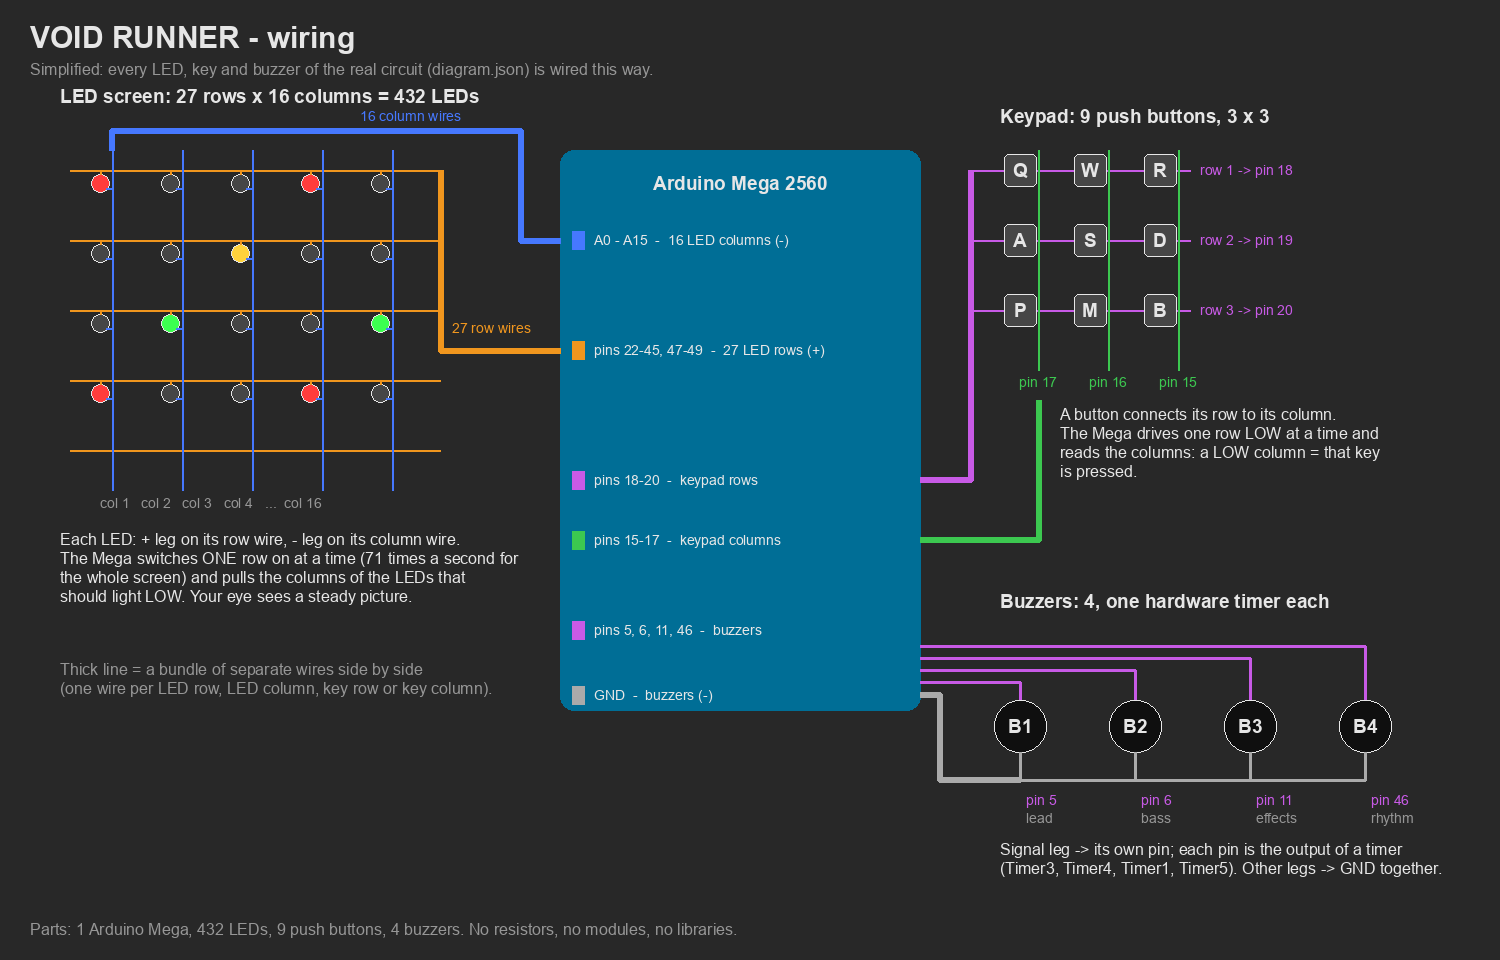
\includegraphics[width=15.00cm]{figures/wiring.png}
\caption{Belongs to pins.h.}
\end{figure}

\subsubsection*{Source code}
\phantomsection\addcontentsline{toc}{subsubsection}{Source code}
\begin{lstlisting}[language=Arduino]
/*
 * pins.h -- GENERATED by tools/gen_circuit.py together with diagram.json.
 * Do not edit by hand: change the generator and run it again, so the circuit
 * and the code always match.
 */
#pragma once
#include <Arduino.h>

// ---- LED screen: 16 columns x 24 game rows + 3 status bars, one big matrix
const uint8_t SCREEN_W    = 16;
const uint8_t SCREEN_H    = 24;
const uint8_t STATUS_ROWS = 3;
const uint8_t TOTAL_ROWS  = SCREEN_H + STATUS_ROWS;

// Anode pin of every LED row: rows 0-23 = game screen top to bottom,
// rows 24-26 = status bars top to bottom (all on the double header).
const uint8_t ROW_PINS[TOTAL_ROWS] = {
  44, 45, 42, 43, 40, 41, 38, 39, 36, 37, 34, 35, 32, 33, 30, 31, 28, 29, 26, 27, 24, 25, 22, 23, 48, 49, 47
};

// Cathode pin of every LED column, left to right: column x is wired to Ax,
// so columns 0-7 are PORTF bits 0-7 and columns 8-15 are PORTK bits 0-7.
const uint8_t COL_PINS[SCREEN_W] = {
  A0, A1, A2, A3, A4, A5, A6, A7, A8, A9, A10, A11, A12, A13, A14, A15
};

// ---- 3 x 3 push-button keypad: contact 1 = row line, contact 2 = column line
const uint8_t KEY_ROWS = 3, KEY_COLS = 3;
const uint8_t KEY_ROW_PINS[KEY_ROWS] = { 18, 19, 20 };
const uint8_t KEY_COL_PINS[KEY_COLS] = { 17, 16, 15 };
const char KEY_NAMES[KEY_ROWS][KEY_COLS] = {
  {'Q', 'W', 'R'},
  {'A', 'S', 'D'},
  {'P', 'M', 'B'}
};

// ---- buzzers, each on the "A" output of its own 16-bit timer
const uint8_t BUZZER_COUNT = 4;
const uint8_t BUZZER_PINS[BUZZER_COUNT] = { 5, 6, 11, 46 };   // Timer3 OC3A, Timer4 OC4A, Timer1 OC1A, Timer5 OC5A
\end{lstlisting}

\clearpage
\subsection*{4.4 display.h – The LED screen}
\phantomsection\addcontentsline{toc}{subsection}{4.4 display.h – The LED screen}
The Timer2 interrupt that lights one LED row at a time (71 full pictures per second), the picture in memory (\texttt{frame}) and every drawing function: pixels, rectangles, bitmaps, letters of the two fonts, numbers, message pages and the status bars. Brightness (100 / 50 / 20 \%) is made by switching the row off early in its time slot.

\begin{figure}[H]\centering
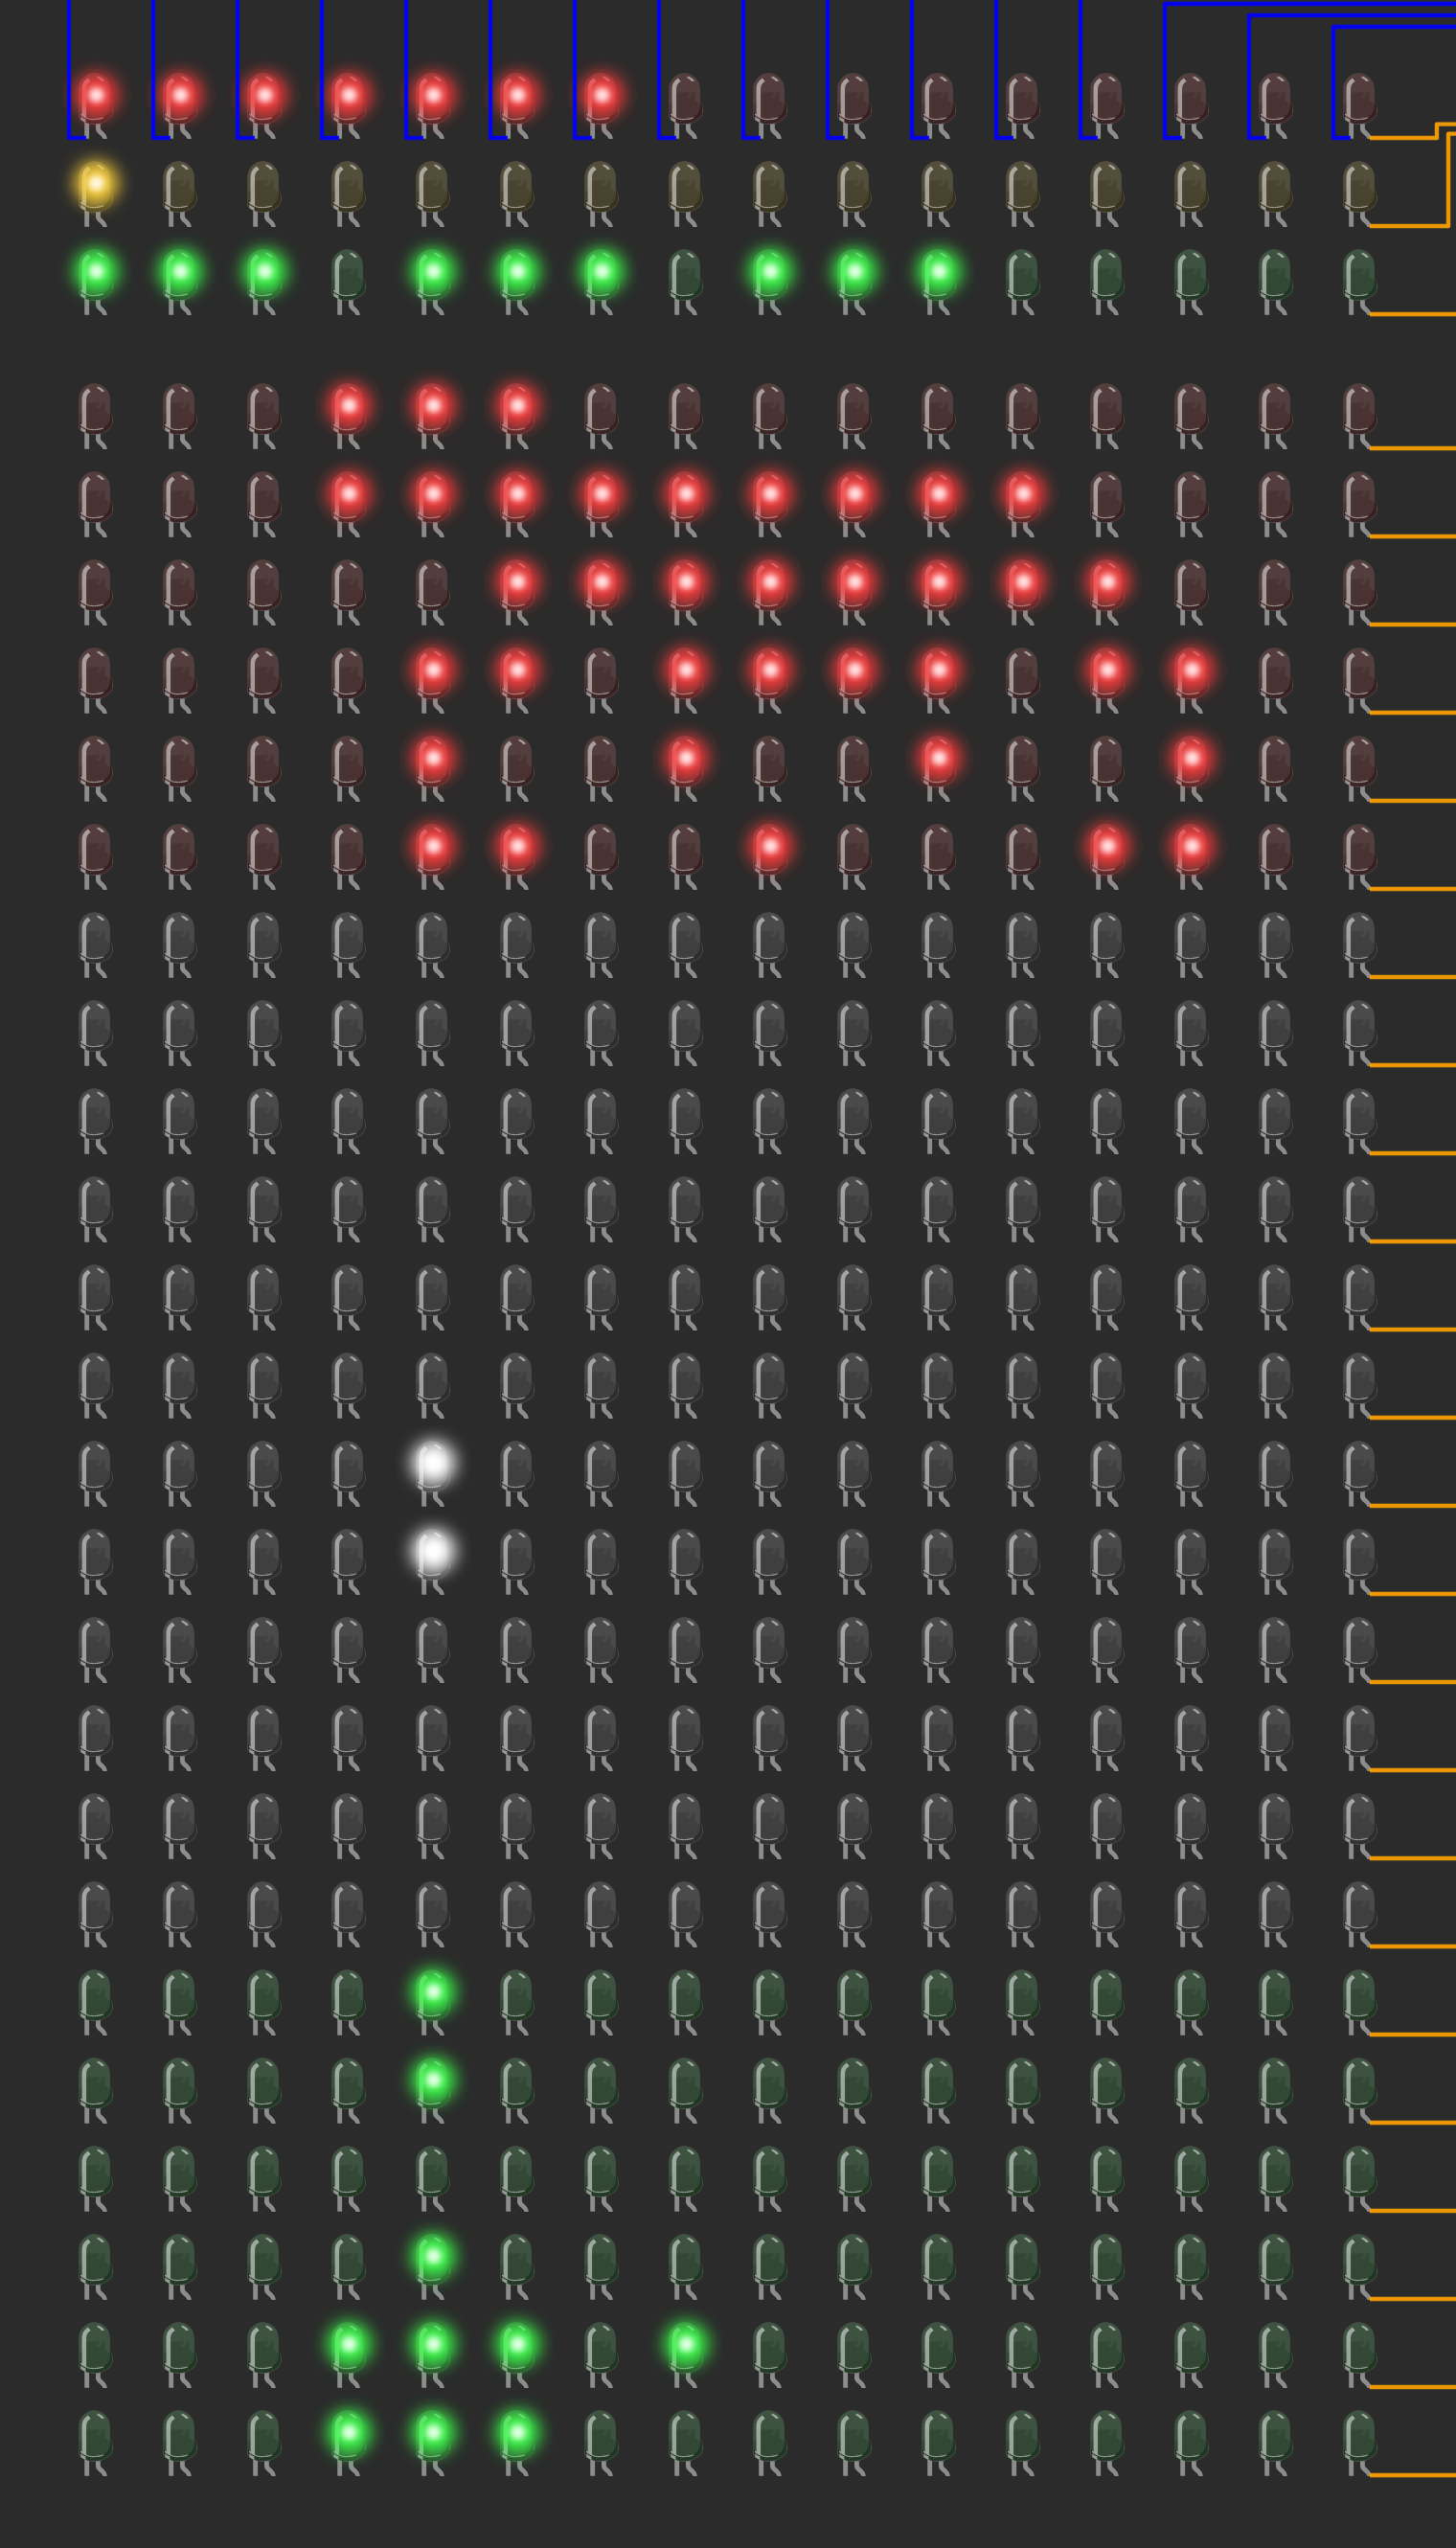
\includegraphics[width=5.00cm]{figures/cu_leds.png}
\caption{Belongs to display.h.}
\end{figure}

{\footnotesize\begin{longtable}{|>{\raggedright\arraybackslash}p{5.82cm}|>{\raggedright\arraybackslash}p{10.68cm}|}
\hline\rowcolor{accent}\textbf{\color{white}Function} & \textbf{\color{white}What it does}\\\hline\endhead
displayBegin() & Starts the LED screen: row and column pins as outputs with every LED off, then Timer2 in CTC mode, so the scan interrupt runs 27 x 71 times per second.\\\hline
\rowcolor{rowshade}displaySetBrightness(uint8\_t percent) & Sets how long each row stays lit inside its time slot (100 = all of it). Below 100 \% the second Timer2 match (COMPB) switches the row off early.\\\hline
present() & Copies the finished picture to the scan buffer in one go, so the interrupt never shows a half-drawn picture.\\\hline
\rowcolor{rowshade}clearScreen() & Switches off every LED of the game screen in \texttt{frame} (the status bars stay).\\\hline
setPixel(int16\_t x, int16\_t y, bool on) & Turns one LED of the game screen on or off in \texttt{frame}, shifted by the screen shake. Pixels outside the screen are ignored, so sprites may stick out at the edges.\\\hline
\rowcolor{rowshade}fillRect(int16\_t x, int16\_t y, int16\_t w, int16\_t h, bool on) & Turns a w x h block of LEDs on or off (bars, ribbons, clearing an area).\\\hline
drawBitmap(int16\_t x, int16\_t y, const uint16\_t* rows, uint8\_t w, uint8\_t h, bool on) & Bitmaps are stored in flash, one 16-bit word per row, leftmost pixel = top bit.\\\hline
\rowcolor{rowshade}drawChar(int16\_t x, int16\_t y, char ch, bool big, uint8\_t scale = 1) & small = 3x5 font (4 pixels per letter), big = 5x7 font (6 pixels per letter). Strings are kept in flash: call with PSTR("TEXT"). Draws one letter or digit with its top-left at (x, y); unknown characters are skipped. scale = 2 draws every pixel as a 2 x 2 block (the big phase number).\\\hline
textWidth(const char* text, bool big) & Width in pixels of a text in the small or big font (for centring).\\\hline
\rowcolor{rowshade}drawText(int16\_t x, int16\_t y, const char* text, bool big) & Draws a text from flash, letter by letter; letters outside the screen are skipped.\\\hline
drawTextCentered(int16\_t y, const char* text, bool big) & Draws a text centred horizontally at row y.\\\hline
\rowcolor{rowshade}pageAt(uint32\_t t, uint8\_t count) & Which page of a sequence of \texttt{count} pages to show t ms after it started (the last one stays).\\\hline
clearRows(int16\_t y, uint8\_t h) & Switches off h rows of the game screen from row y (a clean background for a page).\\\hline
\rowcolor{rowshade}drawPage(const char* line1, const char* line2) & Draws a page of one or two short lines (from flash) in the white zone, rows 6-17, which is cleared first. line2 may be NULL.\\\hline
numberDigits(uint16\_t n) & Counts the digits of a number (for its width).\\\hline
\rowcolor{rowshade}numberWidth(uint16\_t n, bool big) & Width in pixels of a number in the small or big font.\\\hline
drawNumber(int16\_t x, int16\_t y, uint16\_t n, bool big) & Draws a number digit by digit, starting from the right (no leading zeros).\\\hline
\rowcolor{rowshade}drawNumberCentered(int16\_t y, uint16\_t n, bool big) & Draws a number centred horizontally at row y.\\\hline
drawBitmapScaled(int16\_t x, int16\_t y, const uint16\_t* rows, uint8\_t w, uint8\_t h, uint8\_t scale) & Bitmap drawn \texttt{scale} times bigger (ship preview in the hangar).\\\hline
\rowcolor{rowshade}setStatusBits(uint8\_t bar, uint16\_t bits) & Three bars of 16 LEDs above the game screen (matrix rows 24, 25, 26). Sets all 16 LEDs of one bar at once (bit x = LED x).\\\hline
setStatusBar(uint8\_t bar, uint8\_t level) & Fills a status bar from the left with \texttt{level} LEDs (0-16), like a gauge.\\\hline
\rowcolor{rowshade}displayDump() & Prints the picture as text over Serial ('\#' = on), status bars first. Used by the automatic tests (command !d).\\\hline
\end{longtable}}

\subsubsection*{Source code}
\phantomsection\addcontentsline{toc}{subsubsection}{Source code}
\begin{lstlisting}[language=Arduino]
/*
 * display.h -- the LED screen.
 *
 * 16 x 24 game screen + 3 status bars of single LEDs, wired as ONE matrix:
 * 27 rows (LED anodes, pins 22-48) and 16 columns (LED cathodes, A0-A15).
 *
 * The picture lives in `frame`: one 16-bit word per LED row, bit x = column x.
 * A Timer2 interrupt lights one row at a time; all 27 rows are shown 71 times per
 * second, so the picture stays steady whatever the game code is doing.
 *
 * Blinking: Wokwi shows each LED's brightness averaged over 100 ms, so anything that
 * should visibly blink stays on and off for longer than that (frameNo & 8 = 160 ms).
 */
#pragma once
#include "pins.h"
#include "config.h"
#include "font.h"

uint16_t frame[TOTAL_ROWS];              // the game draws here
volatile uint16_t shown[TOTAL_ROWS];     // the scan interrupt shows this copy
volatile uint8_t scanRow = 0;            // row that is lit right now
const uint8_t SCAN_TICK_US = 16;         // Timer2 runs at 16 MHz / 256

// ================================================================= scanning
// Every Timer2 match: old row off, columns of the next row, next row on.
// Column x is wired to pin Ax, so A0-A7 are the bits of PORTF and A8-A15 the bits of
// PORTK: 8 columns are written in one instruction (12 us per row instead of 140 us with
// digitalWrite, measured in Stage 0).
ISR(TIMER2_COMPA_vect) {
  uint8_t row = scanRow;
  digitalWrite(ROW_PINS[row], LOW);
  row = (row + 1 == TOTAL_ROWS) ? 0 : row + 1;
  uint16_t bits = shown[row];
  PORTF = (uint8_t)~lowByte(bits);       // a LOW column lights its LED
  PORTK = (uint8_t)~highByte(bits);
  digitalWrite(ROW_PINS[row], HIGH);
  scanRow = row;
}

// Brightness: a second match part way through the time slot switches the row off early.
ISR(TIMER2_COMPB_vect) {
  digitalWrite(ROW_PINS[scanRow], LOW);
}

// Starts the LED screen: row and column pins as outputs with every LED off, then Timer2
// in CTC mode, so the scan interrupt runs 27 x 71 times per second.
void displayBegin() {
  for (uint8_t r = 0; r < TOTAL_ROWS; r++) {
    pinMode(ROW_PINS[r], OUTPUT);
    digitalWrite(ROW_PINS[r], LOW);
  }
  for (uint8_t x = 0; x < SCREEN_W; x++) {
    pinMode(COL_PINS[x], OUTPUT);
    digitalWrite(COL_PINS[x], HIGH);
  }
  TCCR2A = _BV(WGM21);                   // CTC mode: count 0..OCR2A, then start again
  TCCR2B = _BV(CS22) | _BV(CS21);        // prescaler 256: one count = 16 us
  OCR2A = 1000000UL / ((uint32_t)REFRESH_HZ * TOTAL_ROWS * SCAN_TICK_US) - 1;
  TIMSK2 = _BV(OCIE2A);
}

// Sets how long each row stays lit inside its time slot (100 = all of it). Below 100 %
// the second Timer2 match (COMPB) switches the row off early.
void displaySetBrightness(uint8_t percent) {
  if (percent >= 100) {
    TIMSK2 &= ~_BV(OCIE2B);
    return;
  }
  OCR2B = (uint16_t)(OCR2A + 1) * percent / 100;
  TIMSK2 |= _BV(OCIE2B);
}

// Copies the finished picture to the scan buffer in one go, so the interrupt never
// shows a half-drawn picture.
void present() {
  noInterrupts();
  for (uint8_t r = 0; r < TOTAL_ROWS; r++) shown[r] = frame[r];
  interrupts();
}

// ================================================================= drawing (game screen)
// Switches off every LED of the game screen in `frame` (the status bars stay).
void clearScreen() {
  for (uint8_t y = 0; y < SCREEN_H; y++) frame[y] = 0;
}

int8_t shakeX = 0, shakeY = 0;           // screen shake: everything is drawn shifted

// Turns one LED of the game screen on or off in `frame`, shifted by the screen shake.
// Pixels outside the screen are ignored, so sprites may stick out at the edges.
void setPixel(int16_t x, int16_t y, bool on) {
  x += shakeX;
  y += shakeY;
  if (x < 0 || x >= SCREEN_W || y < 0 || y >= SCREEN_H) return;
  if (on) frame[y] |= 1u << x;
  else frame[y] &= ~(1u << x);
}

// Turns a w x h block of LEDs on or off (bars, ribbons, clearing an area).
void fillRect(int16_t x, int16_t y, int16_t w, int16_t h, bool on) {
  for (int16_t j = y; j < y + h; j++)
    for (int16_t i = x; i < x + w; i++) setPixel(i, j, on);
}

// Bitmaps are stored in flash, one 16-bit word per row, leftmost pixel = top bit.
void drawBitmap(int16_t x, int16_t y, const uint16_t* rows, uint8_t w, uint8_t h, bool on) {
  for (uint8_t r = 0; r < h; r++) {
    uint16_t bits = pgm_read_word(rows + r);
    for (uint8_t c = 0; c < w; c++)
      if (bits & (0x8000u >> c)) setPixel(x + c, y + r, on);
  }
}

// ================================================================= text
// small = 3x5 font (4 pixels per letter), big = 5x7 font (6 pixels per letter).
// Strings are kept in flash: call with PSTR("TEXT").
// Draws one letter or digit with its top-left at (x, y); unknown characters are skipped.
// scale = 2 draws every pixel as a 2 x 2 block (the big phase number).
void drawChar(int16_t x, int16_t y, char ch, bool big, uint8_t scale = 1) {
  const char* chars = big ? FONT5x7_CHARS : FONT3x5_CHARS;
  const char* hit = ch ? strchr_P(chars, ch) : NULL;
  if (!hit) return;
  uint8_t w = big ? 5 : 3, h = big ? 7 : 5;
  const uint8_t* glyph = (big ? FONT5x7 : FONT3x5) + (hit - chars) * w;
  for (uint8_t c = 0; c < w; c++) {
    uint8_t bits = pgm_read_byte(glyph + c);
    for (uint8_t r = 0; r < h; r++)
      if (bits & (1 << r)) fillRect(x + c * scale, y + r * scale, scale, scale, true);
  }
}

// Width in pixels of a text in the small or big font (for centring).
int16_t textWidth(const char* text, bool big) {
  uint8_t n = strlen_P(text);
  return n ? n * (big ? 6 : 4) - 1 : 0;
}

// Draws a text from flash, letter by letter; letters outside the screen are skipped.
void drawText(int16_t x, int16_t y, const char* text, bool big) {
  uint8_t step = big ? 6 : 4;
  for (const char* p = text; char ch = pgm_read_byte(p); p++, x += step)
    if (x > -step && x < SCREEN_W) drawChar(x, y, ch, big);
}

// Draws a text centred horizontally at row y.
void drawTextCentered(int16_t y, const char* text, bool big) {
  drawText((SCREEN_W - textWidth(text, big)) / 2, y, text, big);
}

// ================================================================= pages
// Messages are shown as still "pages" of short words (up to 4 small letters per line),
// one after another, never as scrolling text: Wokwi averages each LED's brightness, so
// moving letters smear into a white block that nobody can read.
const uint16_t PAGE_MS = 900;            // how long one page stays

// Which page of a sequence of `count` pages to show t ms after it started (the last one
// stays).
uint8_t pageAt(uint32_t t, uint8_t count) {
  uint32_t page = t / PAGE_MS;
  return page < count ? page : count - 1;
}

// Switches off h rows of the game screen from row y (a clean background for a page).
void clearRows(int16_t y, uint8_t h) {
  fillRect(0, y, SCREEN_W, h, false);
}

// Draws a page of one or two short lines (from flash) in the white zone, rows 6-17,
// which is cleared first. line2 may be NULL.
void drawPage(const char* line1, const char* line2) {
  clearRows(6, 12);
  if (line2) {
    drawTextCentered(7, line1, false);
    drawTextCentered(13, line2, false);
  } else {
    drawTextCentered(10, line1, false);
  }
}

// ================================================================= numbers
// Counts the digits of a number (for its width).
uint8_t numberDigits(uint16_t n) {
  uint8_t d = 1;
  while (n >= 10) {
    n /= 10;
    d++;
  }
  return d;
}

// Width in pixels of a number in the small or big font.
int16_t numberWidth(uint16_t n, bool big) {
  return numberDigits(n) * (big ? 6 : 4) - 1;
}

// Draws a number digit by digit, starting from the right (no leading zeros).
void drawNumber(int16_t x, int16_t y, uint16_t n, bool big) {
  uint8_t step = big ? 6 : 4;
  for (int8_t i = numberDigits(n) - 1; i >= 0; i--) {
    drawChar(x + i * step, y, '0' + n % 10, big);
    n /= 10;
  }
}

// Draws a number centred horizontally at row y.
void drawNumberCentered(int16_t y, uint16_t n, bool big) {
  drawNumber((SCREEN_W - numberWidth(n, big)) / 2, y, n, big);
}

// Bitmap drawn `scale` times bigger (ship preview in the hangar).
void drawBitmapScaled(int16_t x, int16_t y, const uint16_t* rows, uint8_t w, uint8_t h, uint8_t scale) {
  for (uint8_t r = 0; r < h; r++) {
    uint16_t bits = pgm_read_word(rows + r);
    for (uint8_t c = 0; c < w; c++)
      if (bits & (0x8000u >> c)) fillRect(x + c * scale, y + r * scale, scale, scale, true);
  }
}

// ================================================================= status bars
// Three bars of 16 LEDs above the game screen (matrix rows 24, 25, 26).
// Sets all 16 LEDs of one bar at once (bit x = LED x).
void setStatusBits(uint8_t bar, uint16_t bits) {
  frame[SCREEN_H + bar] = bits;
}

// Fills a status bar from the left with `level` LEDs (0-16), like a gauge.
void setStatusBar(uint8_t bar, uint8_t level) {
  setStatusBits(bar, level >= 16 ? 0xFFFF : (uint16_t)((1u << level) - 1));
}

// ================================================================= test helper
// Prints the picture as text over Serial ('#' = on), status bars first. Used by the
// automatic tests (command !d).
void displayDump() {
  Serial.println(F("[DUMP] begin"));
  for (uint8_t i = 0; i < TOTAL_ROWS; i++) {
    uint8_t r = (i < STATUS_ROWS) ? SCREEN_H + i : i - STATUS_ROWS;   // top to bottom
    if (i == STATUS_ROWS) Serial.println(F("----------------"));
    for (uint8_t x = 0; x < SCREEN_W; x++) Serial.print(frame[r] & (1u << x) ? '#' : '.');
    Serial.println();
  }
  Serial.println(F("[DUMP] end"));
}
\end{lstlisting}

\clearpage
\subsection*{4.5 input.h – The keypad}
\phantomsection\addcontentsline{toc}{subsection}{4.5 input.h – The keypad}
Scans the 3 × 3 push-button matrix row by row, as taught in the course, and debounces every key. It remembers which keys are held and which were just pressed or released, so the other parts can ask "was R just pressed?" or "is D held?".

\begin{figure}[H]\centering
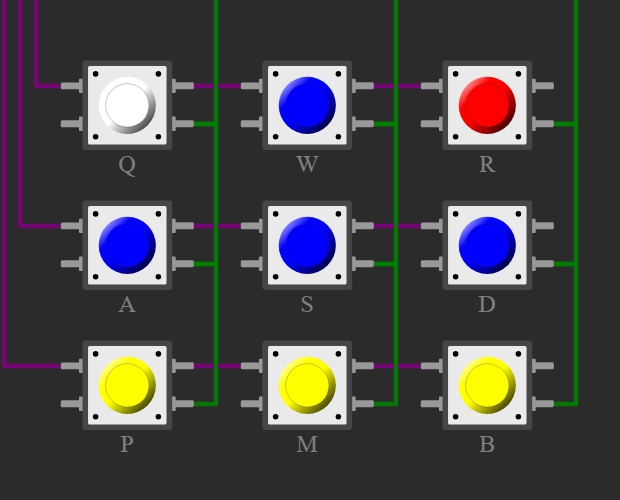
\includegraphics[width=7.00cm]{figures/cu_keypad.png}
\caption{Belongs to input.h.}
\end{figure}

\par\noindent\begin{minipage}{\linewidth}\centering\footnotesize
\begin{tabular}{|>{\raggedright\arraybackslash}p{5.82cm}|>{\raggedright\arraybackslash}p{10.68cm}|}
\hline\rowcolor{accent}\textbf{\color{white}Function} & \textbf{\color{white}What it does}\\\hline
inputBegin() & Sets up the keypad pins: rows switched off (INPUT), columns with pull-up resistors.\\\hline
\rowcolor{rowshade}keyBit(char key) & The bit of a key (by its label, e.g. 'R') in keysHeld and keysPressed.\\\hline
keyHeld(char key) & True while the key is held down.\\\hline
\rowcolor{rowshade}keyPressed(char key) & True only in the picture in which the key went down (one press = one action).\\\hline
inputEndFrame() & Forgets this picture's key presses (called at the end of every picture).\\\hline
\rowcolor{rowshade}readKeys() & Reads the whole keypad once: drives one row LOW at a time and reads the three columns. Returns one bit per key that is down (no debouncing here).\\\hline
inputUpdate(uint32\_t now) & Reads the keypad every 5 ms. A change only counts once the keys read the same four times in a row: that hides the contact bounce that Wokwi simulates.\\\hline
\end{tabular}
\end{minipage}\par\medskip

\subsubsection*{Source code}
\phantomsection\addcontentsline{toc}{subsubsection}{Source code}
\begin{lstlisting}[language=Arduino]
/*
 * input.h -- the 3 x 3 push-button keypad (the 9 keys of the game).
 *
 * Same method as the course: drive one row LOW and read the three columns
 * (INPUT_PULLUP, so a pressed key reads LOW). Rows that are not being read are set to
 * INPUT instead of HIGH: with two keys of one column pressed, a HIGH and a LOW output
 * would otherwise be shorted together through the buttons.
 */
#pragma once
#include "pins.h"

uint16_t keysHeld = 0;                   // debounced: bit (row * 4 + column) = key is down
uint16_t keysPressed = 0;                // keys that went down since the last picture

// Sets up the keypad pins: rows switched off (INPUT), columns with pull-up resistors.
void inputBegin() {
  for (uint8_t r = 0; r < KEY_ROWS; r++) pinMode(KEY_ROW_PINS[r], INPUT);
  for (uint8_t c = 0; c < KEY_COLS; c++) pinMode(KEY_COL_PINS[c], INPUT_PULLUP);
}

// The bit of a key (by its label, e.g. 'R') in keysHeld and keysPressed.
uint16_t keyBit(char key) {
  for (uint8_t i = 0; i < KEY_ROWS * KEY_COLS; i++)
    if (KEY_NAMES[i / KEY_COLS][i % KEY_COLS] == key) return 1u << i;
  return 0;
}

// True while the key is held down.
bool keyHeld(char key) { return keysHeld & keyBit(key); }
// True only in the picture in which the key went down (one press = one action).
bool keyPressed(char key) { return keysPressed & keyBit(key); }
// Forgets this picture's key presses (called at the end of every picture).
void inputEndFrame() { keysPressed = 0; }

// Reads the whole keypad once: drives one row LOW at a time and reads the three columns.
// Returns one bit per key that is down (no debouncing here).
uint16_t readKeys() {
  uint16_t mask = 0;
  for (uint8_t r = 0; r < KEY_ROWS; r++) {
    pinMode(KEY_ROW_PINS[r], OUTPUT);
    digitalWrite(KEY_ROW_PINS[r], LOW);
    delayMicroseconds(5);                // let the line settle
    for (uint8_t c = 0; c < KEY_COLS; c++)
      if (digitalRead(KEY_COL_PINS[c]) == LOW) mask |= 1u << (r * KEY_COLS + c);
    pinMode(KEY_ROW_PINS[r], INPUT);
  }
  return mask;
}

// Reads the keypad every 5 ms. A change only counts once the keys read the same
// four times in a row: that hides the contact bounce that Wokwi simulates.
void inputUpdate(uint32_t now) {
  static uint32_t lastScan = 0;
  static uint16_t candidate = 0;
  static uint8_t sameScans = 0;
  if (now - lastScan < 5) return;
  lastScan = now;
  uint16_t raw = readKeys();
  if (raw != candidate) {
    candidate = raw;
    sameScans = 0;
    return;
  }
  if (sameScans < 3) sameScans++;
  if (sameScans < 3 || candidate == keysHeld) return;
  uint16_t changed = candidate ^ keysHeld;
  keysPressed |= changed & candidate;
  keysHeld = candidate;
  for (uint8_t i = 0; i < KEY_ROWS * KEY_COLS; i++) {
    if (!(changed & (1u << i))) continue;
    Serial.print((keysHeld & (1u << i)) ? F("[KEY] DOWN ") : F("[KEY] UP "));
    Serial.println(KEY_NAMES[i / KEY_COLS][i % KEY_COLS]);
  }
}
\end{lstlisting}

\clearpage
\subsection*{4.6 sound.h – The sound engine}
\phantomsection\addcontentsline{toc}{subsection}{4.6 sound.h – The sound engine}
Drives the four buzzers with four 16-bit timers in CTC toggle mode, so each buzzer plays its note without using processor time. A small music engine plays songs written as note lists (one per voice, looping or once), and an effect engine on voice 3 plays the sound effects with priorities. Mute (M) silences everything.

\begin{figure}[H]\centering
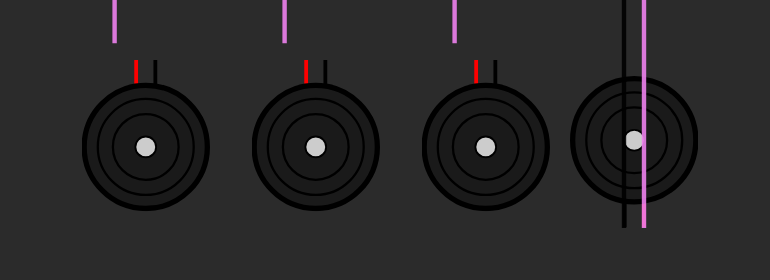
\includegraphics[width=7.00cm]{figures/cu_buzzers.png}
\caption{Belongs to sound.h.}
\end{figure}

{\footnotesize\begin{longtable}{|>{\raggedright\arraybackslash}p{5.82cm}|>{\raggedright\arraybackslash}p{10.68cm}|}
\hline\rowcolor{accent}\textbf{\color{white}Function} & \textbf{\color{white}What it does}\\\hline\endhead
buzzerTone(uint8\_t v, uint16\_t hz) & Makes buzzer v play hz (0 = silent) by setting up its timer; does nothing if it already plays that frequency.\\\hline
\rowcolor{rowshade}soundBegin() & Stops the timers Arduino starts by itself and makes the buzzer pins outputs.\\\hline
noteHz(uint8\_t pitch) & MIDI note number -> frequency: one octave of exact values, halved per octave down.\\\hline
\rowcolor{rowshade}loadNote(Voice\& v) & Copies the voice's current note from flash and works out its length in ms.\\\hline
soundPlaySong(const Track* tracks, uint8\_t tickMs, bool loop) & Starts a song: one track per buzzer (count 0 = that buzzer stays silent), tickMs = length of one tick, loop = start again at the end.\\\hline
\rowcolor{rowshade}songTime() & ms since the song started; the logo uses it so its pictures land on the notes.\\\hline
soundSfx(const SfxPart* parts, uint8\_t count, uint8\_t priority) & Starts a sound effect on buzzer 3, unless a more important one is playing.\\\hline
\rowcolor{rowshade}soundStop() & Stops all music and effects and silences the four buzzers.\\\hline
sfxUpdate(uint32\_t now) & Plays the current effect on buzzer 3: moves on to the next part when one ends, slides the frequency, or jumps to a random frequency every 6 ms (noise for explosions).\\\hline
\rowcolor{rowshade}soundEffect(uint8\_t v, uint16\_t hz) & An effect takes over buzzer v at hz until soundRelease (logo whoosh and crackle).\\\hline
soundRelease(uint8\_t v) & Gives buzzer v back to the music.\\\hline
\rowcolor{rowshade}soundBeep(uint16\_t hz, uint16\_t ms) & A short beep on buzzer 3 (menus, alerts); it replaces any effect.\\\hline
soundSetMuted(bool muted) & Turns all sound off or on (M key); the music keeps running silently.\\\hline
\rowcolor{rowshade}soundUpdate(uint32\_t now) & Call as often as possible: moves every voice on to its next note and drives the buzzers.\\\hline
\end{longtable}}

\subsubsection*{Source code}
\phantomsection\addcontentsline{toc}{subsubsection}{Source code}
\begin{lstlisting}[language=Arduino]
/*
 * sound.h -- four buzzers = four voices.
 *
 * Each buzzer pin is the "A" output of its own 16-bit timer (pin 5 = Timer3, pin 6 =
 * Timer4, pin 11 = Timer1, pin 46 = Timer5). In CTC mode with "toggle on compare match"
 * the timer flips the pin by itself: a note costs no CPU time, and four notes can sound
 * at once (Arduino's tone() can only play one). The Mega has no fifth free timer
 * (Timer0 runs millis(), Timer2 scans the LED screen).
 *
 * Jobs: buzzer 1 = lead, buzzer 2 = bass, buzzer 4 = rhythm guitar / harmony, and
 * buzzer 3 = every sound effect and menu sound (in the short jingles it plays music too). The timers run at 16 MHz / 256: notes up to
 * about C7 stay within 1 % of their pitch, and Wokwi simulates this slow clock far
 * faster than /8 (measured in Stage 0).
 *
 * Music is written as one list of notes per voice (MIDI note numbers, 60 = middle C)
 * with lengths in "ticks". Effects (glides, beeps) take over a voice for a while.
 */
#pragma once
#include "pins.h"

struct TimerRegs {
  volatile uint8_t* tccrA;
  volatile uint8_t* tccrB;
  volatile uint16_t* ocrA;
  volatile uint16_t* tcnt;
};
const TimerRegs VOICE_TIMER[BUZZER_COUNT] = {
  { &TCCR3A, &TCCR3B, &OCR3A, &TCNT3 },  // pin 5  = OC3A
  { &TCCR4A, &TCCR4B, &OCR4A, &TCNT4 },  // pin 6  = OC4A
  { &TCCR1A, &TCCR1B, &OCR1A, &TCNT1 },  // pin 11 = OC1A
  { &TCCR5A, &TCCR5B, &OCR5A, &TCNT5 },  // pin 46 = OC5A
};
const uint8_t SFX_VOICE = 2;             // buzzer 3 (pin 11): sound effects and beeps

struct Note { uint8_t pitch; uint8_t ticks; };   // pitch 0 = rest
struct Track { const Note* notes; uint8_t count; };

struct Voice {
  const Note* notes;                     // track in flash (NULL = no music on this voice)
  uint8_t count, index;
  uint32_t noteStart;
  uint16_t noteMs;
  uint8_t pitch;
  bool effect;                           // an effect has taken over the voice
  uint16_t effectHz;
  uint32_t effectEnd;                    // 0 = until released
  uint16_t playingHz;                    // what the buzzer plays right now
};
Voice voices[BUZZER_COUNT];
uint8_t songTickMs = 50;
uint32_t songStart = 0;
bool songLoops = false;
bool soundMuted = false;
const uint8_t NOTE_GAP_MS = 12;          // short silence at the end of each note

// ================================================================= hardware
// Makes buzzer v play hz (0 = silent) by setting up its timer; does nothing if it already
// plays that frequency.
void buzzerTone(uint8_t v, uint16_t hz) {
  if (soundMuted) hz = 0;
  if (hz == voices[v].playingHz) return;
  voices[v].playingHz = hz;
  const TimerRegs& t = VOICE_TIMER[v];
  *t.tccrB = 0;                          // stop the timer while changing it
  if (hz == 0) {
    *t.tccrA = 0;                        // disconnect the pin from the timer
    digitalWrite(BUZZER_PINS[v], LOW);
    return;
  }
  // Mode bits first: in Arduino's default PWM mode a new OCRnA value would wait for the
  // end of a PWM cycle that a stopped timer never reaches, and the note would be lost.
  *t.tccrA = _BV(COM1A0);                // toggle pin on match (same bit in timers 1, 3, 4, 5)
  *t.tcnt = 0;
  *t.ocrA = F_CPU / (2UL * 256 * hz) - 1;  // f = 16 MHz / (2 * 256 * (OCRnA + 1))
  *t.tccrB = _BV(WGM12) | _BV(CS12);     // CTC mode, prescaler 256: start
}

// Stops the timers Arduino starts by itself and makes the buzzer pins outputs.
void soundBegin() {
  // Arduino starts timers 1, 3, 4 and 5 even when nothing uses them, and Wokwi spends
  // time on every timer count: stop them. A buzzer's timer restarts when it plays.
  // Clearing the A registers too leaves Arduino's PWM mode (see buzzerTone).
  TCCR1B = 0; TCCR1A = 0;
  TCCR3B = 0; TCCR3A = 0;
  TCCR4B = 0; TCCR4A = 0;
  TCCR5B = 0; TCCR5A = 0;
  for (uint8_t v = 0; v < BUZZER_COUNT; v++) pinMode(BUZZER_PINS[v], OUTPUT);
}

// MIDI note number -> frequency: one octave of exact values, halved per octave down.
uint16_t noteHz(uint8_t pitch) {
  static const uint16_t OCTAVE8[12] PROGMEM = {4186, 4435, 4699, 4978, 5274, 5588,
                                               5920, 6272, 6645, 7040, 7459, 7902};
  return pgm_read_word(&OCTAVE8[pitch % 12]) >> (9 - pitch / 12);
}

// ================================================================= music
// Copies the voice's current note from flash and works out its length in ms.
void loadNote(Voice& v) {
  Note n;
  memcpy_P(&n, &v.notes[v.index], sizeof(Note));
  v.pitch = n.pitch;
  v.noteMs = (uint16_t)n.ticks * songTickMs;
}

// Starts a song: one track per buzzer (count 0 = that buzzer stays silent), tickMs =
// length of one tick, loop = start again at the end.
void soundPlaySong(const Track* tracks, uint8_t tickMs, bool loop) {
  uint32_t now = millis();
  songTickMs = tickMs;
  songStart = now;
  songLoops = loop;
  for (uint8_t i = 0; i < BUZZER_COUNT; i++) {
    Voice& v = voices[i];
    v.notes = tracks[i].count ? tracks[i].notes : NULL;
    v.count = tracks[i].count;
    v.index = 0;
    v.noteStart = now;
    if (v.notes) loadNote(v);
  }
}

// ms since the song started; the logo uses it so its pictures land on the notes.
uint32_t songTime() {
  return millis() - songStart;
}

// ================================================================= sound effects (buzzer 3)
// An effect is a short list of parts in flash. Each part slides from one frequency to
// another (fromHz == toHz: a steady tone, 0 Hz: a pause) or, with noise set, jumps to a
// random frequency in that range every few ms (explosions). A new effect only replaces
// the one playing if it is at least as important (priority).
struct SfxPart { uint16_t fromHz, toHz, ms; uint8_t noise; };

const SfxPart* sfxParts = NULL;
uint8_t sfxCount = 0, sfxIndex = 0, sfxPriority = 0;
SfxPart sfxPart;                         // copy of the part playing now
uint32_t sfxPartStart = 0, sfxNoiseAt = 0;
uint16_t sfxNoiseHz = 0;

// Starts a sound effect on buzzer 3, unless a more important one is playing.
void soundSfx(const SfxPart* parts, uint8_t count, uint8_t priority) {
  if (sfxCount && priority < sfxPriority) return;
  sfxParts = parts;
  sfxCount = count;
  sfxIndex = 0;
  sfxPriority = priority;
  sfxPartStart = millis();
  memcpy_P(&sfxPart, &parts[0], sizeof(SfxPart));
}

// Stops all music and effects and silences the four buzzers.
void soundStop() {
  sfxCount = 0;
  for (uint8_t i = 0; i < BUZZER_COUNT; i++) {
    voices[i].notes = NULL;
    voices[i].effect = false;
    buzzerTone(i, 0);
  }
}

// Plays the current effect on buzzer 3: moves on to the next part when one ends, slides
// the frequency, or jumps to a random frequency every 6 ms (noise for explosions).
void sfxUpdate(uint32_t now) {
  if (!sfxCount) return;
  Voice& v = voices[SFX_VOICE];
  while (now - sfxPartStart >= sfxPart.ms) {
    sfxPartStart += sfxPart.ms;
    if (++sfxIndex == sfxCount) {
      sfxCount = 0;
      v.effect = false;
      return;
    }
    memcpy_P(&sfxPart, &sfxParts[sfxIndex], sizeof(SfxPart));
  }
  uint16_t hz;
  if (sfxPart.noise) {
    if ((int32_t)(now - sfxNoiseAt) >= 0) {
      sfxNoiseHz = random(sfxPart.fromHz, sfxPart.toHz);
      sfxNoiseAt = now + 6;
    }
    hz = sfxNoiseHz;
  } else {
    int32_t span = (int32_t)sfxPart.toHz - (int32_t)sfxPart.fromHz;
    hz = sfxPart.fromHz + span * (int32_t)(now - sfxPartStart) / sfxPart.ms;
  }
  v.effect = true;
  v.effectHz = hz;
  v.effectEnd = 0;
}

// ================================================================= effects
// An effect takes over buzzer v at hz until soundRelease (logo whoosh and crackle).
void soundEffect(uint8_t v, uint16_t hz) {
  voices[v].effect = true;
  voices[v].effectHz = hz;
  voices[v].effectEnd = 0;
}

// Gives buzzer v back to the music.
void soundRelease(uint8_t v) {
  voices[v].effect = false;
}

// A short beep on buzzer 3 (menus, alerts); it replaces any effect.
void soundBeep(uint16_t hz, uint16_t ms) {
  sfxCount = 0;                                    // a beep replaces any effect
  Voice& v = voices[SFX_VOICE];
  v.effect = true;
  v.effectHz = hz;
  v.effectEnd = millis() + ms;
  if (v.effectEnd == 0) v.effectEnd = 1;
}

// Turns all sound off or on (M key); the music keeps running silently.
void soundSetMuted(bool muted) {
  soundMuted = muted;
  for (uint8_t i = 0; i < BUZZER_COUNT; i++) buzzerTone(i, 0);
}

// Call as often as possible: moves every voice on to its next note and drives the buzzers.
void soundUpdate(uint32_t now) {
  sfxUpdate(now);
  for (uint8_t i = 0; i < BUZZER_COUNT; i++) {
    Voice& v = voices[i];
    while (v.notes && now - v.noteStart >= v.noteMs) {   // next note (catch up if late)
      v.noteStart += v.noteMs;
      if (++v.index == v.count) {
        if (!songLoops) {
          v.notes = NULL;
          break;
        }
        v.index = 0;
      }
      loadNote(v);
    }
    if (v.effect && v.effectEnd && (int32_t)(now - v.effectEnd) >= 0) v.effect = false;
    uint16_t hz = 0;
    if (v.effect) hz = v.effectHz;
    else if (v.notes && v.pitch && now - v.noteStart < (uint32_t)v.noteMs - NOTE_GAP_MS)
      hz = noteHz(v.pitch);
    buzzerTone(i, hz);
  }
}
\end{lstlisting}

\clearpage
\subsection*{4.7 tunes.h – Songs and sound effects}
\phantomsection\addcontentsline{toc}{subsection}{4.7 tunes.h – Songs and sound effects}
The note lists of every song and the parts of every sound effect, all stored in flash. The four in-game songs are generated by \texttt{tools/compose\_music.py} from a short note notation; the jingles (fanfare, clear, victory, game over) and the effects are written here directly.

\subsubsection*{Source code}
\phantomsection\addcontentsline{toc}{subsubsection}{Source code}
\begin{lstlisting}[language=Arduino]
/*
 * tunes.h -- music and sound effects (all in flash).
 *
 * Songs: one note list per buzzer, MIDI note numbers (60 = middle C, 0 = rest) and
 * lengths in ticks. The in-game songs are original metal tracks: buzzer 1 = lead guitar,
 * buzzer 2 = bass, buzzer 4 = rhythm guitar (a fifth above the bass: a power chord).
 * They leave buzzer 3 to the sound effects, so effects never cut the music. The songs are
 * written in a short notation in tools/compose_music.py, which fills the block below.
 * Effects: parts that slide between two frequencies (or noise for explosions).
 * The start-up melody lives in logo.h.
 */
#pragma once
#include "sound.h"

#define TRACK(notes) {notes, sizeof(notes) / sizeof(Note)}
#define NO_TRACK {NULL, 0}
#define SFX(parts) parts, sizeof(parts) / sizeof(SfxPart)

// ---- BEGIN songs generated by tools/compose_music.py (edit the songs there)
// ================================================================= Phase 1, ROCK BELT: thrash, E minor, galloping bass
// 8 bars, 1 tick = 80 ms, one loop = 10.2 s
const Note PHASE1_LEAD[] PROGMEM = {
  {64, 4}, {67, 2}, {69, 2}, {71, 4}, {69, 2}, {67, 2}, {69, 4}, {67, 2},
  {64, 2}, {62, 4}, {64, 4}, {64, 4}, {67, 2}, {69, 2}, {71, 4}, {74, 2},
  {76, 2}, {70, 4}, {69, 4}, {67, 4}, {66, 4}, {76, 6}, {74, 2}, {71, 4},
  {67, 4}, {69, 6}, {71, 2}, {67, 4}, {64, 4}, {76, 2}, {74, 2}, {71, 2},
  {69, 2}, {67, 2}, {69, 2}, {71, 2}, {74, 2}, {66, 8}, {71, 8},
};
const Note PHASE1_BASS[] PROGMEM = {
  {40, 2}, {40, 1}, {40, 1}, {40, 2}, {40, 1}, {40, 1}, {40, 2}, {40, 1},
  {40, 1}, {40, 2}, {40, 1}, {40, 1}, {40, 2}, {40, 1}, {40, 1}, {40, 2},
  {40, 1}, {40, 1}, {43, 2}, {43, 1}, {43, 1}, {45, 2}, {45, 1}, {45, 1},
  {40, 2}, {40, 1}, {40, 1}, {40, 2}, {40, 1}, {40, 1}, {40, 2}, {40, 1},
  {40, 1}, {40, 2}, {40, 1}, {40, 1}, {40, 2}, {40, 1}, {40, 1}, {40, 2},
  {40, 1}, {40, 1}, {46, 4}, {45, 4}, {40, 2}, {40, 1}, {40, 1}, {40, 2},
  {40, 1}, {40, 1}, {40, 2}, {40, 1}, {40, 1}, {40, 2}, {40, 1}, {40, 1},
  {40, 2}, {40, 1}, {40, 1}, {40, 2}, {40, 1}, {40, 1}, {43, 2}, {43, 1},
  {43, 1}, {45, 2}, {45, 1}, {45, 1}, {48, 2}, {48, 1}, {48, 1}, {48, 2},
  {48, 1}, {48, 1}, {47, 2}, {47, 1}, {47, 1}, {47, 2}, {47, 1}, {47, 1},
  {47, 2}, {47, 1}, {47, 1}, {47, 2}, {47, 1}, {47, 1}, {47, 8},
};
const Note PHASE1_RHYTHM[] PROGMEM = {
  {47, 2}, {47, 1}, {47, 1}, {47, 2}, {47, 1}, {47, 1}, {47, 2}, {47, 1},
  {47, 1}, {47, 2}, {47, 1}, {47, 1}, {47, 2}, {47, 1}, {47, 1}, {47, 2},
  {47, 1}, {47, 1}, {50, 2}, {50, 1}, {50, 1}, {52, 2}, {52, 1}, {52, 1},
  {47, 2}, {47, 1}, {47, 1}, {47, 2}, {47, 1}, {47, 1}, {47, 2}, {47, 1},
  {47, 1}, {47, 2}, {47, 1}, {47, 1}, {47, 2}, {47, 1}, {47, 1}, {47, 2},
  {47, 1}, {47, 1}, {53, 4}, {52, 4}, {47, 2}, {47, 1}, {47, 1}, {47, 2},
  {47, 1}, {47, 1}, {47, 2}, {47, 1}, {47, 1}, {47, 2}, {47, 1}, {47, 1},
  {47, 2}, {47, 1}, {47, 1}, {47, 2}, {47, 1}, {47, 1}, {50, 2}, {50, 1},
  {50, 1}, {52, 2}, {52, 1}, {52, 1}, {55, 2}, {55, 1}, {55, 1}, {55, 2},
  {55, 1}, {55, 1}, {54, 2}, {54, 1}, {54, 1}, {54, 2}, {54, 1}, {54, 1},
  {54, 2}, {54, 1}, {54, 1}, {54, 2}, {54, 1}, {54, 1}, {54, 8},
};
const Track SONG_PHASE1[BUZZER_COUNT] = {TRACK(PHASE1_LEAD), TRACK(PHASE1_BASS), NO_TRACK, TRACK(PHASE1_RHYTHM)};
const uint8_t SONG_PHASE1_TICK_MS = 80;

// ================================================================= Phase 2, DEEP MIST: slow drop-D chugs, D minor
// 8 bars, 1 tick = 100 ms, one loop = 12.8 s
const Note PHASE2_LEAD[] PROGMEM = {
  {0, 8}, {69, 4}, {65, 4}, {64, 8}, {62, 4}, {0, 4}, {0, 8}, {69, 4},
  {72, 4}, {70, 8}, {69, 4}, {0, 4}, {74, 6}, {72, 2}, {69, 4}, {65, 4},
  {67, 6}, {69, 2}, {64, 8}, {65, 4}, {64, 4}, {62, 4}, {61, 4}, {62, 12},
  {0, 4},
};
const Note PHASE2_BASS[] PROGMEM = {
  {38, 1}, {38, 1}, {0, 1}, {38, 1}, {38, 2}, {0, 2}, {38, 1}, {38, 1},
  {0, 1}, {38, 1}, {41, 2}, {40, 2}, {38, 1}, {38, 1}, {0, 1}, {38, 1},
  {38, 2}, {0, 2}, {45, 4}, {44, 2}, {43, 2}, {38, 1}, {38, 1}, {0, 1},
  {38, 1}, {38, 2}, {0, 2}, {38, 1}, {38, 1}, {0, 1}, {38, 1}, {41, 2},
  {40, 2}, {38, 1}, {38, 1}, {0, 1}, {38, 1}, {38, 2}, {0, 2}, {45, 4},
  {44, 2}, {43, 2}, {38, 1}, {38, 1}, {0, 1}, {38, 1}, {38, 2}, {0, 2},
  {38, 1}, {38, 1}, {0, 1}, {38, 1}, {41, 2}, {40, 2}, {38, 1}, {38, 1},
  {0, 1}, {38, 1}, {38, 2}, {0, 2}, {45, 4}, {44, 2}, {43, 2}, {38, 1},
  {38, 1}, {0, 1}, {38, 1}, {38, 2}, {0, 2}, {38, 1}, {38, 1}, {0, 1},
  {38, 1}, {41, 2}, {40, 2}, {46, 8}, {45, 8},
};
const Note PHASE2_RHYTHM[] PROGMEM = {
  {45, 1}, {45, 1}, {0, 1}, {45, 1}, {45, 2}, {0, 2}, {45, 1}, {45, 1},
  {0, 1}, {45, 1}, {48, 2}, {47, 2}, {45, 1}, {45, 1}, {0, 1}, {45, 1},
  {45, 2}, {0, 2}, {52, 4}, {51, 2}, {50, 2}, {45, 1}, {45, 1}, {0, 1},
  {45, 1}, {45, 2}, {0, 2}, {45, 1}, {45, 1}, {0, 1}, {45, 1}, {48, 2},
  {47, 2}, {45, 1}, {45, 1}, {0, 1}, {45, 1}, {45, 2}, {0, 2}, {52, 4},
  {51, 2}, {50, 2}, {45, 1}, {45, 1}, {0, 1}, {45, 1}, {45, 2}, {0, 2},
  {45, 1}, {45, 1}, {0, 1}, {45, 1}, {48, 2}, {47, 2}, {45, 1}, {45, 1},
  {0, 1}, {45, 1}, {45, 2}, {0, 2}, {52, 4}, {51, 2}, {50, 2}, {45, 1},
  {45, 1}, {0, 1}, {45, 1}, {45, 2}, {0, 2}, {45, 1}, {45, 1}, {0, 1},
  {45, 1}, {48, 2}, {47, 2}, {53, 8}, {52, 8},
};
const Track SONG_PHASE2[BUZZER_COUNT] = {TRACK(PHASE2_LEAD), TRACK(PHASE2_BASS), NO_TRACK, TRACK(PHASE2_RHYTHM)};
const uint8_t SONG_PHASE2_TICK_MS = 100;

// ================================================================= Phase 3, THE VOID: syncopated groove, E minor
// 8 bars, 1 tick = 75 ms, one loop = 9.6 s
const Note PHASE3_LEAD[] PROGMEM = {
  {71, 4}, {71, 2}, {67, 2}, {69, 4}, {64, 4}, {71, 4}, {71, 2}, {67, 2},
  {72, 4}, {71, 4}, {71, 4}, {71, 2}, {67, 2}, {69, 4}, {64, 2}, {67, 2},
  {66, 4}, {67, 4}, {69, 4}, {71, 4}, {76, 4}, {74, 2}, {71, 2}, {74, 4},
  {76, 4}, {79, 4}, {78, 2}, {76, 2}, {74, 4}, {71, 4}, {76, 2}, {71, 2},
  {67, 2}, {64, 2}, {76, 2}, {71, 2}, {67, 2}, {64, 2}, {76, 1}, {74, 1},
  {71, 1}, {69, 1}, {67, 1}, {69, 1}, {71, 1}, {74, 1}, {76, 8},
};
const Note PHASE3_BASS[] PROGMEM = {
  {40, 1}, {0, 1}, {40, 1}, {0, 1}, {40, 1}, {40, 1}, {0, 2}, {43, 2},
  {40, 2}, {46, 2}, {45, 2}, {40, 1}, {0, 1}, {40, 1}, {0, 1}, {40, 1},
  {40, 1}, {0, 2}, {48, 4}, {47, 4}, {40, 1}, {0, 1}, {40, 1}, {0, 1},
  {40, 1}, {40, 1}, {0, 2}, {43, 2}, {40, 2}, {46, 2}, {45, 2}, {40, 1},
  {0, 1}, {40, 1}, {0, 1}, {40, 1}, {40, 1}, {0, 2}, {48, 4}, {47, 4},
  {40, 1}, {0, 1}, {40, 1}, {0, 1}, {40, 1}, {40, 1}, {0, 2}, {43, 2},
  {40, 2}, {46, 2}, {45, 2}, {40, 1}, {0, 1}, {40, 1}, {0, 1}, {40, 1},
  {40, 1}, {0, 2}, {48, 4}, {47, 4}, {40, 2}, {40, 2}, {40, 2}, {40, 2},
  {40, 2}, {40, 2}, {40, 2}, {40, 2}, {40, 1}, {40, 1}, {40, 1}, {40, 1},
  {40, 1}, {40, 1}, {40, 1}, {40, 1}, {40, 1}, {40, 1}, {40, 1}, {40, 1},
  {40, 1}, {40, 1}, {40, 1}, {40, 1},
};
const Note PHASE3_RHYTHM[] PROGMEM = {
  {47, 1}, {0, 1}, {47, 1}, {0, 1}, {47, 1}, {47, 1}, {0, 2}, {50, 2},
  {47, 2}, {53, 2}, {52, 2}, {47, 1}, {0, 1}, {47, 1}, {0, 1}, {47, 1},
  {47, 1}, {0, 2}, {55, 4}, {54, 4}, {47, 1}, {0, 1}, {47, 1}, {0, 1},
  {47, 1}, {47, 1}, {0, 2}, {50, 2}, {47, 2}, {53, 2}, {52, 2}, {47, 1},
  {0, 1}, {47, 1}, {0, 1}, {47, 1}, {47, 1}, {0, 2}, {55, 4}, {54, 4},
  {47, 1}, {0, 1}, {47, 1}, {0, 1}, {47, 1}, {47, 1}, {0, 2}, {50, 2},
  {47, 2}, {53, 2}, {52, 2}, {47, 1}, {0, 1}, {47, 1}, {0, 1}, {47, 1},
  {47, 1}, {0, 2}, {55, 4}, {54, 4}, {47, 2}, {47, 2}, {47, 2}, {47, 2},
  {47, 2}, {47, 2}, {47, 2}, {47, 2}, {47, 1}, {47, 1}, {47, 1}, {47, 1},
  {47, 1}, {47, 1}, {47, 1}, {47, 1}, {47, 1}, {47, 1}, {47, 1}, {47, 1},
  {47, 1}, {47, 1}, {47, 1}, {47, 1},
};
const Track SONG_PHASE3[BUZZER_COUNT] = {TRACK(PHASE3_LEAD), TRACK(PHASE3_BASS), NO_TRACK, TRACK(PHASE3_RHYTHM)};
const uint8_t SONG_PHASE3_TICK_MS = 75;

// ================================================================= Boss fights: tremolo bass, chromatic lead
// 4 bars, 1 tick = 70 ms, one loop = 4.5 s
const Note BOSS_LEAD[] PROGMEM = {
  {76, 2}, {77, 2}, {76, 2}, {75, 2}, {76, 8}, {77, 2}, {79, 2}, {77, 2},
  {76, 2}, {77, 8}, {79, 2}, {81, 2}, {82, 2}, {81, 2}, {79, 4}, {76, 4},
  {70, 4}, {69, 4}, {68, 4}, {67, 4},
};
const Note BOSS_BASS[] PROGMEM = {
  {40, 1}, {40, 1}, {40, 1}, {40, 1}, {40, 1}, {40, 1}, {40, 1}, {40, 1},
  {40, 1}, {40, 1}, {40, 1}, {40, 1}, {40, 1}, {40, 1}, {40, 1}, {40, 1},
  {41, 1}, {41, 1}, {41, 1}, {41, 1}, {41, 1}, {41, 1}, {41, 1}, {41, 1},
  {41, 1}, {41, 1}, {41, 1}, {41, 1}, {41, 1}, {41, 1}, {41, 1}, {41, 1},
  {40, 1}, {40, 1}, {40, 1}, {40, 1}, {40, 1}, {40, 1}, {40, 1}, {40, 1},
  {43, 1}, {43, 1}, {43, 1}, {43, 1}, {46, 1}, {46, 1}, {46, 1}, {46, 1},
  {46, 1}, {46, 1}, {46, 1}, {46, 1}, {46, 1}, {46, 1}, {46, 1}, {46, 1},
  {45, 1}, {45, 1}, {45, 1}, {45, 1}, {45, 1}, {45, 1}, {45, 1}, {45, 1},
};
const Note BOSS_RHYTHM[] PROGMEM = {
  {47, 1}, {47, 1}, {47, 1}, {47, 1}, {47, 1}, {47, 1}, {47, 1}, {47, 1},
  {47, 1}, {47, 1}, {47, 1}, {47, 1}, {47, 1}, {47, 1}, {47, 1}, {47, 1},
  {48, 1}, {48, 1}, {48, 1}, {48, 1}, {48, 1}, {48, 1}, {48, 1}, {48, 1},
  {48, 1}, {48, 1}, {48, 1}, {48, 1}, {48, 1}, {48, 1}, {48, 1}, {48, 1},
  {47, 1}, {47, 1}, {47, 1}, {47, 1}, {47, 1}, {47, 1}, {47, 1}, {47, 1},
  {50, 1}, {50, 1}, {50, 1}, {50, 1}, {53, 1}, {53, 1}, {53, 1}, {53, 1},
  {53, 1}, {53, 1}, {53, 1}, {53, 1}, {53, 1}, {53, 1}, {53, 1}, {53, 1},
  {52, 1}, {52, 1}, {52, 1}, {52, 1}, {52, 1}, {52, 1}, {52, 1}, {52, 1},
};
const Track SONG_BOSS[BUZZER_COUNT] = {TRACK(BOSS_LEAD), TRACK(BOSS_BASS), NO_TRACK, TRACK(BOSS_RHYTHM)};
const uint8_t SONG_BOSS_TICK_MS = 70;
// ---- END songs generated by tools/compose_music.py

// ================================================================= short tunes (play once)
const Note STING_A[] PROGMEM = {{69, 2}, {76, 2}, {81, 4}};       // a phase begins
const Note STING_B[] PROGMEM = {{64, 2}, {69, 2}, {76, 4}};
const Note STING_C[] PROGMEM = {{45, 8}};
const Track SONG_STING[BUZZER_COUNT] = {TRACK(STING_A), TRACK(STING_B), TRACK(STING_C)};

const Note CLEAR_A[] PROGMEM = {{76, 2}, {79, 2}, {84, 6}};       // a phase is cleared
const Note CLEAR_B[] PROGMEM = {{72, 2}, {76, 2}, {79, 6}};
const Note CLEAR_C[] PROGMEM = {{48, 10}};
const Track SONG_CLEAR[BUZZER_COUNT] = {TRACK(CLEAR_A), TRACK(CLEAR_B), TRACK(CLEAR_C)};

const Note WIN_A[] PROGMEM = {{72, 2}, {76, 2}, {79, 2}, {84, 6}, {81, 2}, {83, 2}, {84, 8}};
const Note WIN_B[] PROGMEM = {{64, 2}, {67, 2}, {72, 2}, {76, 6}, {77, 2}, {79, 2}, {76, 8}};
const Note WIN_C[] PROGMEM = {{48, 6}, {55, 6}, {53, 4}, {48, 8}};
const Track SONG_VICTORY[BUZZER_COUNT] = {TRACK(WIN_A), TRACK(WIN_B), TRACK(WIN_C)};

const Note OVER_A[] PROGMEM = {{64, 4}, {63, 4}, {62, 4}, {61, 12}};
const Note OVER_B[] PROGMEM = {{57, 4}, {56, 4}, {55, 4}, {52, 12}};
const Note OVER_C[] PROGMEM = {{45, 12}, {40, 12}};
const Track SONG_GAMEOVER[BUZZER_COUNT] = {TRACK(OVER_A), TRACK(OVER_B), TRACK(OVER_C)};

// ================================================================= sound effects (buzzer 3)
// {from Hz, to Hz, ms, noise}; priorities: 1 shot ... 6 player hit
const SfxPart SFX_SHOT[] PROGMEM = {{2200, 1300, 35, 0}};
const SfxPart SFX_CHIRP[] PROGMEM = {{1500, 2600, 40, 0}};                  // auto-fire starts
const SfxPart SFX_EMPTY[] PROGMEM = {{2600, 2600, 8, 0}};                   // dry click
const SfxPart SFX_HIT[] PROGMEM = {{900, 650, 40, 0}};                      // enemy hit
const SfxPart SFX_BOOM[] PROGMEM = {{200, 900, 180, 1}};                    // enemy destroyed
const SfxPart SFX_BIG_BOOM[] PROGMEM = {{100, 600, 500, 1}, {600, 80, 300, 0}};
const SfxPart SFX_PLAYER_HIT[] PROGMEM = {{1200, 150, 350, 0}, {80, 300, 250, 1}};
const SfxPart SFX_PICKUP[] PROGMEM = {{800, 1600, 70, 0}, {1600, 2400, 70, 0}};
const SfxPart SFX_LIFE[] PROGMEM = {{660, 660, 80, 0}, {880, 880, 80, 0}, {1320, 1320, 140, 0}};
const SfxPart SFX_LOW_AMMO[] PROGMEM = {{1100, 1100, 60, 0}, {0, 0, 50, 0}, {1100, 1100, 60, 0}};
const SfxPart SFX_SIREN[] PROGMEM = {
  {600, 1200, 250, 0}, {1200, 600, 250, 0}, {600, 1200, 250, 0},
  {1200, 600, 250, 0}, {600, 1200, 250, 0}, {1200, 600, 250, 0},
};
const SfxPart SFX_ROAR[] PROGMEM = {{90, 400, 600, 1}};                     // boss changes form
const SfxPart SFX_TEST[] PROGMEM = {{400, 2000, 900, 0}};                   // LED test sweep
\end{lstlisting}

\clearpage
\subsection*{4.8 storage.h – EEPROM: settings and best score}
\phantomsection\addcontentsline{toc}{subsection}{4.8 storage.h – EEPROM: settings and best score}
Saves the chosen ship, the difficulty, the brightness, the sound setting and the best score (with the zone it reached and its difficulty) in the Mega's EEPROM, using the EEPROM registers directly. A check byte tells whether the EEPROM holds valid data.

\begin{figure}[H]\centering
\begin{minipage}[t]{3.40cm}\centering
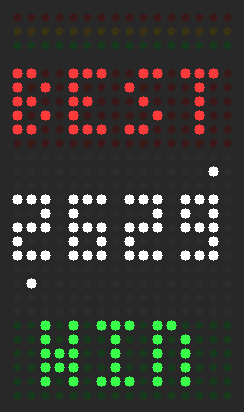
\includegraphics[width=\linewidth]{figures/best1.png}\\[-2pt]
{\scriptsize\color{grey}}
\end{minipage}\hspace{4pt}%
\begin{minipage}[t]{3.40cm}\centering
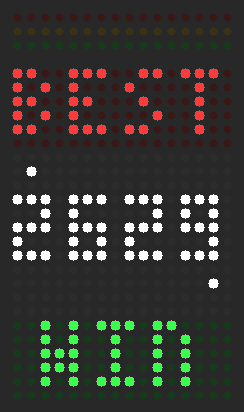
\includegraphics[width=\linewidth]{figures/best3.png}\\[-2pt]
{\scriptsize\color{grey}}
\end{minipage}\hspace{4pt}%
\caption{What storage.h draws or uses.}
\end{figure}

\par\noindent\begin{minipage}{\linewidth}\centering\footnotesize
\begin{tabular}{|>{\raggedright\arraybackslash}p{5.82cm}|>{\raggedright\arraybackslash}p{10.68cm}|}
\hline\rowcolor{accent}\textbf{\color{white}Function} & \textbf{\color{white}What it does}\\\hline
eepromRead(uint16\_t address) & Reads one byte of the EEPROM (first waits if a write is still busy).\\\hline
\rowcolor{rowshade}eepromWrite(uint16\_t address, uint8\_t value) & Writes one byte to the EEPROM, only if it changed (saves time and EEPROM wear).\\\hline
settingsSave() & Saves the settings and the best score: a marker byte, then the Settings struct.\\\hline
\rowcolor{rowshade}settingsLoad() & Loads the settings at start-up. If the EEPROM holds none (new chip, new simulation) or a value is out of range, the defaults are used.\\\hline
\end{tabular}
\end{minipage}\par\medskip

\subsubsection*{Source code}
\phantomsection\addcontentsline{toc}{subsubsection}{Source code}
\begin{lstlisting}[language=Arduino]
/*
 * storage.h -- settings and the high score, kept in the Mega's EEPROM.
 *
 * Written with the EEPROM registers directly (no library):
 *   EEAR = address, EEDR = data byte,
 *   EECR: EERE starts a read; EEMPE then EEPE (within 4 clock cycles) starts a write.
 * A write takes about 3.4 ms, so the next access waits while EEPE is still set.
 * (Wokwi keeps the EEPROM while a simulation runs; a restart starts empty.)
 */
#pragma once
#include "config.h"

struct Settings {
  uint8_t brightness;                    // index into BRIGHTNESS_LEVELS
  uint8_t muted;
  uint8_t difficulty;
  uint8_t ship;                          // chosen in the hangar
  uint16_t best;                         // high score
  uint8_t bestPhase;                     // phase reached with the high score (4 = won)
  uint8_t bestDifficulty;                // difficulty the high score was made on
};
Settings settings;
const uint8_t EE_MAGIC = 0xA7;           // marks an EEPROM that holds our settings

// Reads one byte of the EEPROM (first waits if a write is still busy).
uint8_t eepromRead(uint16_t address) {
  while (EECR & _BV(EEPE)) {}            // wait for a write in progress
  EEAR = address;
  EECR |= _BV(EERE);
  return EEDR;
}

// Writes one byte to the EEPROM, only if it changed (saves time and EEPROM wear).
void eepromWrite(uint16_t address, uint8_t value) {
  if (eepromRead(address) == value) return;   // saves EEPROM wear (and time)
  EEAR = address;
  EEDR = value;
  noInterrupts();                        // EEPE must follow EEMPE within 4 cycles
  EECR |= _BV(EEMPE);
  EECR |= _BV(EEPE);
  interrupts();
}

// Saves the settings and the best score: a marker byte, then the Settings struct.
void settingsSave() {
  eepromWrite(0, EE_MAGIC);
  const uint8_t* p = (const uint8_t*)&settings;
  for (uint8_t i = 0; i < sizeof(Settings); i++) eepromWrite(1 + i, p[i]);
}

// Loads the settings at start-up. If the EEPROM holds none (new chip, new simulation) or
// a value is out of range, the defaults are used.
void settingsLoad() {
  settings = {0, 0, DIFF_NORMAL, 0, 0, 0, DIFF_EASY};
  if (eepromRead(0) == EE_MAGIC) {
    uint8_t* p = (uint8_t*)&settings;
    for (uint8_t i = 0; i < sizeof(Settings); i++) p[i] = eepromRead(1 + i);
  }
  if (settings.brightness >= sizeof(BRIGHTNESS_LEVELS)) settings.brightness = 0;
  if (settings.difficulty > DIFF_HARD) settings.difficulty = DIFF_NORMAL;
  if (settings.ship > 2) settings.ship = 0;
  if (settings.bestDifficulty > DIFF_HARD) settings.bestDifficulty = DIFF_EASY;
  settings.muted = settings.muted ? 1 : 0;
}
\end{lstlisting}

\clearpage
\subsection*{4.9 font.h – Fonts (generated)}
\phantomsection\addcontentsline{toc}{subsection}{4.9 font.h – Fonts (generated)}
Two pixel fonts: small 3 × 5 letters (four fit on a line) and big 5 × 7 letters and digits. They are drawn as ASCII art in \texttt{tools/gen\_font.py}, which writes this file.

\begin{figure}[H]\centering
\begin{minipage}[t]{3.40cm}\centering
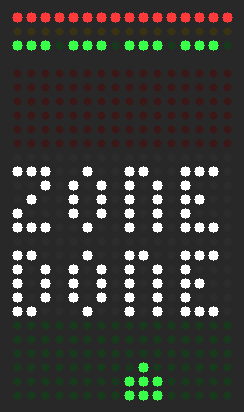
\includegraphics[width=\linewidth]{figures/zonedone.png}\\[-2pt]
{\scriptsize\color{grey}}
\end{minipage}\hspace{4pt}%
\begin{minipage}[t]{3.40cm}\centering
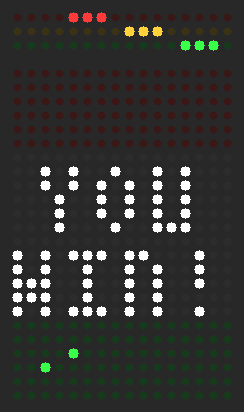
\includegraphics[width=\linewidth]{figures/vic_d.png}\\[-2pt]
{\scriptsize\color{grey}}
\end{minipage}\hspace{4pt}%
\caption{What font.h draws or uses.}
\end{figure}

\subsubsection*{Source code}
\phantomsection\addcontentsline{toc}{subsubsection}{Source code}
\begin{lstlisting}[language=Arduino]
/*
 * font.h -- GENERATED by tools/gen_font.py (the letters are drawn there as ASCII art).
 * Each glyph is stored column by column, one byte per column, bit 0 = top row.
 */
#pragma once
#include <avr/pgmspace.h>

// 3 x 5 font: glyph i is the i-th character of FONT3x5_CHARS
const char FONT3x5_CHARS[] PROGMEM = "ABCDEFGHIJKLMNOPQRSTUVWXYZ0123456789 -!:.>";
const uint8_t FONT3x5[] PROGMEM = {
  0x1E, 0x05, 0x1E,  // 'A'
  0x1F, 0x15, 0x0A,  // 'B'
  0x0E, 0x11, 0x11,  // 'C'
  0x1F, 0x11, 0x0E,  // 'D'
  0x1F, 0x15, 0x11,  // 'E'
  0x1F, 0x05, 0x01,  // 'F'
  0x0E, 0x11, 0x1D,  // 'G'
  0x1F, 0x04, 0x1F,  // 'H'
  0x11, 0x1F, 0x11,  // 'I'
  0x08, 0x10, 0x0F,  // 'J'
  0x1F, 0x04, 0x1B,  // 'K'
  0x1F, 0x10, 0x10,  // 'L'
  0x1F, 0x06, 0x1F,  // 'M'
  0x1F, 0x01, 0x1E,  // 'N'
  0x0E, 0x11, 0x0E,  // 'O'
  0x1F, 0x05, 0x02,  // 'P'
  0x0E, 0x19, 0x16,  // 'Q'
  0x1F, 0x05, 0x1A,  // 'R'
  0x12, 0x15, 0x09,  // 'S'
  0x01, 0x1F, 0x01,  // 'T'
  0x1F, 0x10, 0x1F,  // 'U'
  0x0F, 0x10, 0x0F,  // 'V'
  0x1F, 0x0C, 0x1F,  // 'W'
  0x1B, 0x04, 0x1B,  // 'X'
  0x03, 0x1C, 0x03,  // 'Y'
  0x19, 0x15, 0x13,  // 'Z'
  0x1F, 0x11, 0x1F,  // '0'
  0x12, 0x1F, 0x10,  // '1'
  0x1D, 0x15, 0x17,  // '2'
  0x15, 0x15, 0x1F,  // '3'
  0x07, 0x04, 0x1F,  // '4'
  0x17, 0x15, 0x1D,  // '5'
  0x1F, 0x15, 0x1D,  // '6'
  0x01, 0x1D, 0x03,  // '7'
  0x1F, 0x15, 0x1F,  // '8'
  0x17, 0x15, 0x1F,  // '9'
  0x00, 0x00, 0x00,  // ' '
  0x04, 0x04, 0x04,  // '-'
  0x00, 0x17, 0x00,  // '!'
  0x00, 0x0A, 0x00,  // ':'
  0x00, 0x10, 0x00,  // '.'
  0x1F, 0x0E, 0x04,  // '>'
};

// 5 x 7 font: glyph i is the i-th character of FONT5x7_CHARS
const char FONT5x7_CHARS[] PROGMEM = " !-.:0123456789ABCDEFGHIJKLMNOPQRSTUVWXYZ";
const uint8_t FONT5x7[] PROGMEM = {
  0x00, 0x00, 0x00, 0x00, 0x00,  // ' '
  0x00, 0x00, 0x5F, 0x00, 0x00,  // '!'
  0x08, 0x08, 0x08, 0x08, 0x08,  // '-'
  0x00, 0x60, 0x60, 0x00, 0x00,  // '.'
  0x00, 0x36, 0x36, 0x00, 0x00,  // ':'
  0x3E, 0x51, 0x49, 0x45, 0x3E,  // '0'
  0x00, 0x42, 0x7F, 0x40, 0x00,  // '1'
  0x42, 0x61, 0x51, 0x49, 0x46,  // '2'
  0x21, 0x41, 0x45, 0x4B, 0x31,  // '3'
  0x18, 0x14, 0x12, 0x7F, 0x10,  // '4'
  0x27, 0x45, 0x45, 0x45, 0x39,  // '5'
  0x3C, 0x4A, 0x49, 0x49, 0x30,  // '6'
  0x01, 0x71, 0x09, 0x05, 0x03,  // '7'
  0x36, 0x49, 0x49, 0x49, 0x36,  // '8'
  0x06, 0x49, 0x49, 0x29, 0x1E,  // '9'
  0x7E, 0x09, 0x09, 0x09, 0x7E,  // 'A'
  0x7F, 0x49, 0x49, 0x49, 0x36,  // 'B'
  0x3E, 0x41, 0x41, 0x41, 0x22,  // 'C'
  0x7F, 0x41, 0x41, 0x41, 0x3E,  // 'D'
  0x7F, 0x49, 0x49, 0x49, 0x41,  // 'E'
  0x7F, 0x09, 0x09, 0x09, 0x01,  // 'F'
  0x3E, 0x41, 0x49, 0x49, 0x7A,  // 'G'
  0x7F, 0x08, 0x08, 0x08, 0x7F,  // 'H'
  0x00, 0x41, 0x7F, 0x41, 0x00,  // 'I'
  0x20, 0x40, 0x41, 0x3F, 0x01,  // 'J'
  0x7F, 0x08, 0x14, 0x22, 0x41,  // 'K'
  0x7F, 0x40, 0x40, 0x40, 0x40,  // 'L'
  0x7F, 0x02, 0x0C, 0x02, 0x7F,  // 'M'
  0x7F, 0x04, 0x08, 0x10, 0x7F,  // 'N'
  0x3E, 0x41, 0x41, 0x41, 0x3E,  // 'O'
  0x7F, 0x09, 0x09, 0x09, 0x06,  // 'P'
  0x3E, 0x41, 0x51, 0x21, 0x5E,  // 'Q'
  0x7F, 0x09, 0x19, 0x29, 0x46,  // 'R'
  0x46, 0x49, 0x49, 0x49, 0x31,  // 'S'
  0x01, 0x01, 0x7F, 0x01, 0x01,  // 'T'
  0x3F, 0x40, 0x40, 0x40, 0x3F,  // 'U'
  0x1F, 0x20, 0x40, 0x20, 0x1F,  // 'V'
  0x7F, 0x20, 0x18, 0x20, 0x7F,  // 'W'
  0x63, 0x14, 0x08, 0x14, 0x63,  // 'X'
  0x03, 0x04, 0x78, 0x04, 0x03,  // 'Y'
  0x61, 0x51, 0x49, 0x45, 0x43,  // 'Z'
};
\end{lstlisting}

\clearpage
\subsection*{4.10 art.h – Pixel art}
\phantomsection\addcontentsline{toc}{subsection}{4.10 art.h – Pixel art}
Every picture of the game as binary numbers: one 16-bit word per row, the 1s are the lit pixels. The three ships, the enemies, the rocks, the pickups, the bosses, the warning sign and the letters of the logo.

\begin{figure}[H]\centering
\begin{minipage}[t]{2.80cm}\centering

\includegraphics[width=\linewidth]{figures/sprite_ship_bolt.png}\\[-2pt]
{\scriptsize\color{grey}}
\end{minipage}\hspace{4pt}%
\begin{minipage}[t]{2.80cm}\centering

\includegraphics[width=\linewidth]{figures/sprite_ship_dart.png}\\[-2pt]
{\scriptsize\color{grey}}
\end{minipage}\hspace{4pt}%
\begin{minipage}[t]{2.80cm}\centering

\includegraphics[width=\linewidth]{figures/sprite_ship_twin.png}\\[-2pt]
{\scriptsize\color{grey}}
\end{minipage}\hspace{4pt}%
\begin{minipage}[t]{2.80cm}\centering

\includegraphics[width=\linewidth]{figures/sprite_enemy_cruiser.png}\\[-2pt]
{\scriptsize\color{grey}}
\end{minipage}\hspace{4pt}%
\begin{minipage}[t]{2.80cm}\centering

\includegraphics[width=\linewidth]{figures/sprite_boss_warden.png}\\[-2pt]
{\scriptsize\color{grey}}
\end{minipage}\hspace{4pt}%
\caption{What art.h draws or uses.}
\end{figure}

\subsubsection*{Source code}
\phantomsection\addcontentsline{toc}{subsubsection}{Source code}
\begin{lstlisting}[language=Arduino]
/*
 * art.h -- pixel art, stored in flash. One 16-bit word per row, the leftmost pixel is
 * the top bit, so the 1s in each binary number draw the picture.
 */
#pragma once
#include <avr/pgmspace.h>

// ================================================================= the player's ships (3 x 3)
const uint16_t SHIP_BOLT[3] PROGMEM = {        // BOLT: balanced
  0b0100000000000000,                          //  .#.
  0b1110000000000000,                          //  ###
  0b1110000000000000,                          //  ###
};
const uint16_t SHIP_DART[3] PROGMEM = {        // DART: fast
  0b0100000000000000,                          //  .#.
  0b1110000000000000,                          //  ###
  0b1010000000000000,                          //  #.#
};
const uint16_t SHIP_TWIN[3] PROGMEM = {        // TWIN: two guns
  0b1010000000000000,                          //  #.#
  0b1110000000000000,                          //  ###
  0b1110000000000000,                          //  ###
};
const uint16_t SHIP_LEFT[3] PROGMEM = {        // BOLT flying left (logo)
  0b0110000000000000,                          //  .##
  0b1110000000000000,                          //  ###
  0b0110000000000000,                          //  .##
};
const uint16_t* const SHIP_UP = SHIP_BOLT;

// ================================================================= enemies and rocks
const uint16_t ENEMY_DRONE[2] PROGMEM = {      // drone: slow, shoots straight down
  0b1010000000000000,                          //  #.#
  0b0100000000000000,                          //  .#.
};
const uint16_t ENEMY_WEAVER[2] PROGMEM = {     // weaver: zig-zags
  0b1110000000000000,                          //  ###
  0b1010000000000000,                          //  #.#
};
const uint16_t ENEMY_MINER[2] PROGMEM = {      // mine-layer: crosses the top, drops mines
  0b1110000000000000,                          //  ###
  0b0100000000000000,                          //  .#.
};
const uint16_t ENEMY_CRUISER[3] PROGMEM = {    // cruiser: tough, aims at you
  0b0111000000000000,                          //  .###.
  0b1101100000000000,                          //  ##.##
  0b1010100000000000,                          //  #.#.#
};
// Rocks are hollow and lumpy (a crater in the middle), so they don't look like any ship.
const uint16_t ROCK_SMALL[3] PROGMEM = {
  0b1100000000000000,                          //  ##.
  0b1010000000000000,                          //  #.#
  0b0110000000000000,                          //  .##
};
const uint16_t ROCK_BIG[3] PROGMEM = {         // breaks into two small rocks
  0b0110000000000000,                          //  .##.
  0b1101000000000000,                          //  ##.#
  0b0110000000000000,                          //  .##.
};


// ================================================================= pickups (blinking)
const uint16_t PICKUP_AMMO[3] PROGMEM = {      // ammo crate: solid, unlike the hollow rocks
  0b1110000000000000,                          //  ###
  0b1110000000000000,                          //  ###
  0b1110000000000000,                          //  ###
};
const uint16_t PICKUP_LIFE[3] PROGMEM = {      // extra life
  0b0100000000000000,                          //  .#.
  0b1110000000000000,                          //  ###
  0b0100000000000000,                          //  .#.
};

// ================================================================= bosses
const uint16_t BOSS_WARDEN[4] PROGMEM = {      // phase 1: wide and slow, spread shots
  0b0011111100000000,                          //  ..######..
  0b0111111110000000,                          //  .########.
  0b1101111011000000,                          //  ##.####.##
  0b1001001001000000,                          //  #..#..#..#
};
const uint16_t BOSS_HUNTER[3] PROGMEM = {      // phase 2: small and fast, dashes and charges
  0b1000100000000000,                          //  #...#
  0b1111100000000000,                          //  #####
  0b0101000000000000,                          //  .#.#.
};
const uint16_t BOSS_KING[5] PROGMEM = {        // phase 3: the Void King, first form
  0b0011111111000000,                          //  ..########..
  0b0111111111100000,                          //  .##########.
  0b1110011001110000,                          //  ###..##..###
  0b1111111111110000,                          //  ############
  0b0101010101010000,                          //  .#.#.#.#.#.#
};
const uint16_t BOSS_KING_ANGRY[5] PROGMEM = {  // second form: the eye opens
  0b1011111111010000,                          //  #.########.#
  0b0111100111100000,                          //  .####..####.
  0b1110100101110000,                          //  ###.#..#.###
  0b1111111111110000,                          //  ############
  0b1010100101010000,                          //  #.#.#..#.#.#
};

// ================================================================= signs
const uint16_t WARNING_SIGN[10] PROGMEM = {    // 11 x 10, shown before each boss
  0b0000010000000000,                          //  .....#.....
  0b0000101000000000,                          //  ....#.#....
  0b0000101000000000,                          //  ....#.#....
  0b0001000100000000,                          //  ...#...#...
  0b0001010100000000,                          //  ...#.#.#...
  0b0010010010000000,                          //  ..#..#..#..
  0b0010010010000000,                          //  ..#..#..#..
  0b0100000001000000,                          //  .#.......#.
  0b0100010001000000,                          //  .#...#...#.
  0b1111111111100000,                          //  ###########
};

// ================================================================= logo: "VOID", bold 10 x 5 letters
const uint8_t LOGO_W = 10, LOGO_H = 5, LOGO_X = 3;
const uint8_t LOGO_Y[4] = {0, 6, 12, 18};      // V in the red band ... D in the green band
const uint16_t LOGO_LETTERS[4][LOGO_H] PROGMEM = {
  {                                            // V
    0b1100000011000000,                        //  ##......##
    0b0110000110000000,                        //  .##....##.
    0b0011001100000000,                        //  ..##..##..
    0b0001111000000000,                        //  ...####...
    0b0000110000000000,                        //  ....##....
  },
  {                                            // O
    0b0111111110000000,                        //  .########.
    0b1100000011000000,                        //  ##......##
    0b1100000011000000,                        //  ##......##
    0b1100000011000000,                        //  ##......##
    0b0111111110000000,                        //  .########.
  },
  {                                            // I
    0b0011111100000000,                        //  ..######..
    0b0000110000000000,                        //  ....##....
    0b0000110000000000,                        //  ....##....
    0b0000110000000000,                        //  ....##....
    0b0011111100000000,                        //  ..######..
  },
  {                                            // D
    0b1111111000000000,                        //  #######...
    0b1100001100000000,                        //  ##....##..
    0b1100000110000000,                        //  ##.....##.
    0b1100001100000000,                        //  ##....##..
    0b1111111000000000,                        //  #######...
  },
};
\end{lstlisting}

\clearpage
\subsection*{4.11 logo.h – Start-up logo and welcome melody}
\phantomsection\addcontentsline{toc}{subsection}{4.11 logo.h – Start-up logo and welcome melody}
The 5.6-second logo animation and its melody. The picture is driven by the song's own clock, so every movement lands on a note: warp, the ship, the VOID letters, "RUNNER" on a ribbon, the flash and the glowing sign.

\begin{figure}[H]\centering
\begin{minipage}[t]{3.20cm}\centering
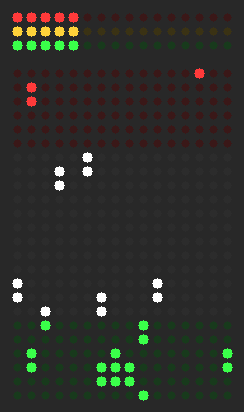
\includegraphics[width=\linewidth]{figures/logo_ship.png}\\[-2pt]
{\scriptsize\color{grey}}
\end{minipage}\hspace{4pt}%
\begin{minipage}[t]{3.20cm}\centering
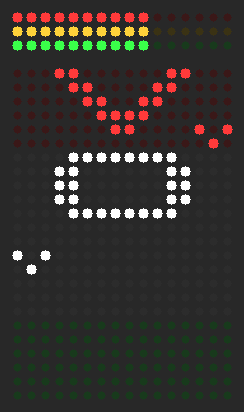
\includegraphics[width=\linewidth]{figures/logo_letters.png}\\[-2pt]
{\scriptsize\color{grey}}
\end{minipage}\hspace{4pt}%
\begin{minipage}[t]{3.20cm}\centering
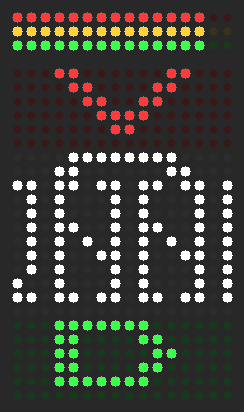
\includegraphics[width=\linewidth]{figures/logo_runner.png}\\[-2pt]
{\scriptsize\color{grey}}
\end{minipage}\hspace{4pt}%
\caption{What logo.h draws or uses.}
\end{figure}

\par\noindent\begin{minipage}{\linewidth}\centering\footnotesize
\begin{tabular}{|>{\raggedright\arraybackslash}p{5.82cm}|>{\raggedright\arraybackslash}p{10.68cm}|}
\hline\rowcolor{accent}\textbf{\color{white}Function} & \textbf{\color{white}What it does}\\\hline
drawLogoLetter(uint8\_t i) & Draws letter i of the VOID sign (V, O, I, D from top to bottom).\\\hline
\rowcolor{rowshade}logoBegin() & Starts the logo: scatters the warp stars and starts the welcome melody.\\\hline
starSpeed(uint32\_t t) & Star speed in 1/16 pixel per picture: speeds up, brakes, then drifts.\\\hline
\rowcolor{rowshade}drawStars(uint32\_t t) & Moves and draws the warp stars; the faster they fly, the longer their streaks.\\\hline
drawShipUp(int16\_t x, int16\_t y, uint16\_t frameNo) & Draws the ship flying up, with a flickering engine flame below it.\\\hline
\rowcolor{rowshade}logoEffects(uint32\_t t) & Sound effects that follow the picture: whoosh, glide and letter crackle.\\\hline
logoUpdate(uint16\_t frameNo) & Draws one picture of the logo. Returns true when the logo is over.\\\hline
\end{tabular}
\end{minipage}\par\medskip

\subsubsection*{Source code}
\phantomsection\addcontentsline{toc}{subsubsection}{Source code}
\begin{lstlisting}[language=Arduino]
/*
 * logo.h -- the start-up logo, played in sync with the welcome melody.
 *
 * The picture is driven by the song's own clock (songTime()), so every movement lands
 * on its note. Timeline (ms):
 *     0 - 1200  warp: star streaks rush past and speed up      rising "whoosh" + low drone
 *  1200 - 2000  the ship rises from the bottom and brakes       3 falling braking notes
 *  2000 - 2400  the ship shoots up and out of the screen        quick rising glide
 *  2400 - 3600  V, O, I, D light up one by one, flickering on;  one note per letter
 *               enemy drones fly past in the side margins       + crackle while it flickers
 *  3600 - 4800  "RUNNER" crosses on a dark ribbon, towed by     melody, harmony and bass
 *               the ship
 *  4800 - 5600  the whole screen flashes, then the sign glows   final A-minor chord
 * The status bars fill up during the logo like a start-up progress bar.
 */
#pragma once
#include "display.h"
#include "sound.h"
#include "art.h"

// ---- welcome melody: one track per buzzer, 1 tick = 50 ms (MIDI note numbers)
const Note BOOT_MELODY[] PROGMEM = {
  {0, 24},                                          // warp (whoosh is an effect)
  {0, 16},                                          // ship arrives
  {0, 8},                                           // ship leaves (glide is an effect)
  {69, 6}, {72, 6}, {76, 6}, {81, 6},               // V O I D: A4 C5 E5 A5
  {76, 3}, {74, 3}, {72, 3}, {74, 3}, {76, 3}, {76, 3}, {76, 6},   // RUNNER tune
  {76, 8}, {0, 8},                                  // final chord, top note E5
};
const Note BOOT_HARMONY[] PROGMEM = {
  {0, 24},
  {64, 4}, {60, 4}, {57, 6}, {0, 2},                // braking: E4 C4 A3
  {0, 32},
  {72, 6}, {71, 6}, {69, 6}, {71, 6},               // C5 B4 A4 B4
  {72, 8}, {0, 8},                                  // final chord, middle note C5
};
const Note BOOT_BASS[] PROGMEM = {
  {45, 24},                                         // A2 drone under the warp
  {0, 24},
  {0, 24},                                          // (crackle effects)
  {45, 3}, {45, 3}, {52, 3}, {45, 3}, {45, 3}, {45, 3}, {43, 3}, {45, 3},  // bass line
  {57, 8}, {0, 8},                                  // final chord, low note A3
};
const Track BOOT_SONG[BUZZER_COUNT] = {
  {BOOT_MELODY, sizeof(BOOT_MELODY) / sizeof(Note)},
  {BOOT_HARMONY, sizeof(BOOT_HARMONY) / sizeof(Note)},
  {BOOT_BASS, sizeof(BOOT_BASS) / sizeof(Note)},
};
const uint8_t BOOT_TICK_MS = 50;
const uint16_t LOGO_END_MS = 5600;
const uint16_t LETTER_START[4] = {2400, 2700, 3000, 3300};
const uint8_t LETTER_FLICKER_MS = 120;

// ---- warp stars: y is stored in 1/16 pixel so they can move smoothly
const uint8_t STAR_COUNT = 12;
int8_t starX[STAR_COUNT];
int16_t starY16[STAR_COUNT];

// Draws letter i of the VOID sign (V, O, I, D from top to bottom).
void drawLogoLetter(uint8_t i) {
  drawBitmap(LOGO_X, LOGO_Y[i], LOGO_LETTERS[i], LOGO_W, LOGO_H, true);
}

// Starts the logo: scatters the warp stars and starts the welcome melody.
void logoBegin() {
  for (uint8_t i = 0; i < STAR_COUNT; i++) {
    starX[i] = random(SCREEN_W);
    starY16[i] = random(SCREEN_H * 16);
  }
  soundPlaySong(BOOT_SONG, BOOT_TICK_MS, false);
}

// Star speed in 1/16 pixel per picture: speeds up, brakes, then drifts.
uint8_t starSpeed(uint32_t t) {
  if (t < 1200) return 4 + 28 * t / 1200;
  if (t < 2000) return 32 - 29 * (t - 1200) / 800;
  return 3;
}

// Moves and draws the warp stars; the faster they fly, the longer their streaks.
void drawStars(uint32_t t) {
  uint8_t speed = starSpeed(t);
  uint8_t len = 1 + speed / 10;                    // faster = longer streak
  for (uint8_t i = 0; i < STAR_COUNT; i++) {
    starY16[i] += speed;
    if (starY16[i] / 16 - len > SCREEN_H) {        // fell off the bottom: start again on top
      starY16[i] = -16 * (int16_t)random(4);
      starX[i] = random(SCREEN_W);
    }
    for (uint8_t k = 0; k < len; k++) setPixel(starX[i], starY16[i] / 16 - k, true);
  }
}

// Draws the ship flying up, with a flickering engine flame below it.
void drawShipUp(int16_t x, int16_t y, uint16_t frameNo) {
  drawBitmap(x, y, SHIP_UP, 3, 3, true);
  if (frameNo & 1) setPixel(x + 1, y + 3, true);   // flickering engine flame
}

// Sound effects that follow the picture: whoosh, glide and letter crackle.
void logoEffects(uint32_t t) {
  if (t < 1200) soundEffect(0, 150 + 1350 * t / 1200);
  else if (t >= 2000 && t < 2300) soundEffect(0, 400 + 1200 * (t - 2000) / 300);
  else soundRelease(0);
  bool crackle = false;
  for (uint8_t i = 0; i < 4; i++)
    if (t >= LETTER_START[i] && t < LETTER_START[i] + LETTER_FLICKER_MS) crackle = true;
  if (crackle) soundEffect(2, random(1500, 3500));
  else soundRelease(2);
}

// Draws one picture of the logo. Returns true when the logo is over.
bool logoUpdate(uint16_t frameNo) {
  uint32_t t = songTime();
  if (t >= LOGO_END_MS) {
    soundRelease(0);
    soundRelease(2);
    return true;
  }
  logoEffects(t);
  clearScreen();
  if (t < 2400) drawStars(t);
  if (t >= 1200 && t < 2000) {                     // ship rises and brakes
    uint32_t p = (t - 1200) * 100 / 800, rest = 100 - p;
    drawShipUp(6, 19 + 5 * rest * rest / 10000, frameNo);
  } else if (t >= 2000 && t < 2400) {              // ship shoots up and out
    uint32_t q = (t - 2000) * 100 / 400;
    int16_t y = 19 - (int16_t)(23 * q * q / 10000);
    drawShipUp(6, y, frameNo);
    setPixel(7, y + 4, true);                      // longer flame
  }
  if (t >= LETTER_START[0] && t < 4800) {
    for (uint8_t i = 0; i < 4; i++) {              // letters light up, flickering at first
      if (t < LETTER_START[i]) continue;
      uint32_t age = t - LETTER_START[i];
      if (age >= LETTER_FLICKER_MS || (age / 30) % 2 == 0) drawLogoLetter(i);
    }
    if (t < 3600) {                                // drones fly past in the side margins
      drawBitmap(0, -2 + (int16_t)((t - 2400) * 26 / 1200), ENEMY_DRONE, 3, 2, true);
      if (t >= 2800) drawBitmap(13, -2 + (int16_t)((t - 2800) * 26 / 1200), ENEMY_DRONE, 3, 2, true);
    }
  }
  if (t >= 3600 && t < 4800) {                     // "RUNNER" on a dark ribbon, towed by the ship
    fillRect(0, 8, SCREEN_W, 9, false);
    for (uint8_t x = 0; x < SCREEN_W; x++)
      if ((x + t / 60) % 3) {                      // ribbon edges move like a conveyor
        setPixel(x, 8, true);
        setPixel(x, 16, true);
      }
    int16_t x = 16 - (int16_t)((t - 3600) * 51 / 1200);
    drawText(x, 9, PSTR("RUNNER"), true);
    drawBitmap(x - 4, 11, SHIP_LEFT, 3, 3, true);
  }
  if (t >= 4800) {                                 // final hit: flash, then the sign glows
    if (t < 4900) fillRect(0, 0, SCREEN_W, SCREEN_H, true);
    else for (uint8_t i = 0; i < 4; i++) drawLogoLetter(i);
  }
  uint8_t level = t >= 4800 ? 16 : t * 16 / 4800;  // status bars: start-up progress
  for (uint8_t b = 0; b < STATUS_ROWS; b++) setStatusBar(b, level);
  return false;
}
\end{lstlisting}

\clearpage
\subsection*{4.12 title.h – Title screen}
\phantomsection\addcontentsline{toc}{subsection}{4.12 title.h – Title screen}
The VOID sign stays lit, ships keep flying past it, and every 7 seconds a banner shows the pages "PUSH", a big R, "TO", "PLAY". After 20 s without a key the demo starts.

\begin{figure}[H]\centering
\begin{minipage}[t]{3.40cm}\centering
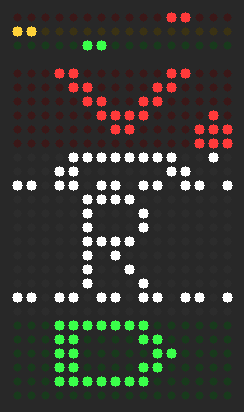
\includegraphics[width=\linewidth]{figures/title.png}\\[-2pt]
{\scriptsize\color{grey}}
\end{minipage}\hspace{4pt}%
\begin{minipage}[t]{3.40cm}\centering
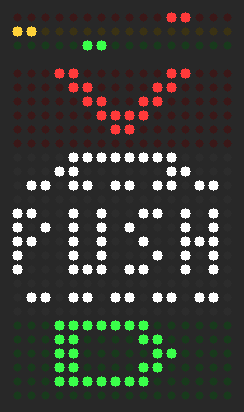
\includegraphics[width=\linewidth]{figures/title_push.png}\\[-2pt]
{\scriptsize\color{grey}}
\end{minipage}\hspace{4pt}%
\caption{What title.h draws or uses.}
\end{figure}

\par\noindent\begin{minipage}{\linewidth}\centering\footnotesize
\begin{tabular}{|>{\raggedright\arraybackslash}p{5.82cm}|>{\raggedright\arraybackslash}p{10.68cm}|}
\hline\rowcolor{accent}\textbf{\color{white}Function} & \textbf{\color{white}What it does}\\\hline
titleDraw(uint32\_t t, uint16\_t frameNo) & Draws one picture of the title screen at time t (ms since it opened).\\\hline
\end{tabular}
\end{minipage}\par\medskip

\subsubsection*{Source code}
\phantomsection\addcontentsline{toc}{subsubsection}{Source code}
\begin{lstlisting}[language=Arduino]
/*
 * title.h -- title screen: the VOID sign stays lit, ships keep flying past it, and every
 * 7 seconds a banner shows the pages "PUSH", a big R, "TO", "PLAY".
 */
#pragma once
#include "display.h"
#include "art.h"
#include "logo.h"

// Draws one picture of the title screen at time t (ms since it opened).
void titleDraw(uint32_t t, uint16_t frameNo) {
  clearScreen();
  for (uint8_t i = 0; i < 4; i++) drawLogoLetter(i);
  drawBitmap(0, -2 + (int16_t)(t % 2400 * 26 / 2400), ENEMY_DRONE, 3, 2, true);   // drone down the left
  int16_t shipY = 24 - (int16_t)(t % 2000 * 28 / 2000);                          // ship up the right
  drawBitmap(13, shipY, SHIP_UP, 3, 3, true);
  if (frameNo & 1) setPixel(14, shipY + 3, true);
  uint32_t b = t % 7000;
  if (b < 4 * PAGE_MS) {                           // the banner: PUSH, R, TO, PLAY
    fillRect(0, 8, SCREEN_W, 9, false);
    for (uint8_t x = 0; x < SCREEN_W; x++)
      if ((x + t / 60) % 3) {
        setPixel(x, 8, true);
        setPixel(x, 16, true);
      }
    uint8_t page = b / PAGE_MS;
    if (page == 1) drawChar(5, 9, 'R', true);     // the big R, 5 x 7
    else drawTextCentered(10, page == 0 ? PSTR("PUSH") : page == 2 ? PSTR("TO") : PSTR("PLAY"), false);
  }
  for (uint8_t bar = 0; bar < STATUS_ROWS; bar++) {      // status bars: a slow chase
    uint8_t head = (t / 120 + bar * 5) % 16;
    setStatusBits(bar, (1u << head) | (1u << ((head + 15) % 16)));
  }
}
\end{lstlisting}

\clearpage
\subsection*{4.13 menu.h – Main menu}
\phantomsection\addcontentsline{toc}{subsection}{4.13 menu.h – Main menu}
The menu PLAY, SHIP, OPTS, BEST: W/S move the underline, R opens the item, Q goes back to the title.

\begin{figure}[H]\centering
\begin{minipage}[t]{3.60cm}\centering
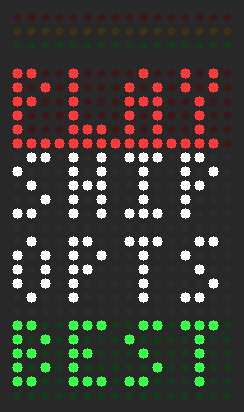
\includegraphics[width=\linewidth]{figures/menu.png}\\[-2pt]
{\scriptsize\color{grey}}
\end{minipage}\hspace{4pt}%
\caption{What menu.h draws or uses.}
\end{figure}

\par\noindent\begin{minipage}{\linewidth}\centering\footnotesize
\begin{tabular}{|>{\raggedright\arraybackslash}p{5.82cm}|>{\raggedright\arraybackslash}p{10.68cm}|}
\hline\rowcolor{accent}\textbf{\color{white}Function} & \textbf{\color{white}What it does}\\\hline
menuItem(uint8\_t i) & Text of menu item i (the list of texts is stored in flash).\\\hline
\rowcolor{rowshade}menuUpdate() & Handles the keys; returns the item to open, MENU\_BACK or MENU\_NONE.\\\hline
menuDraw() & Draws the four menu items, underlines the chosen one and switches the status bars off.\\\hline
\end{tabular}
\end{minipage}\par\medskip

\subsubsection*{Source code}
\phantomsection\addcontentsline{toc}{subsubsection}{Source code}
\begin{lstlisting}[language=Arduino]
/*
 * menu.h -- main menu: PLAY, SHIP, OPTS, BEST (W/S to choose, R to open, Q back).
 * The chosen item is underlined.
 */
#pragma once
#include "display.h"
#include "input.h"
#include "sound.h"

const char MENU_PLAY[] PROGMEM = "PLAY";
const char MENU_SHIP[] PROGMEM = "SHIP";
const char MENU_OPTS[] PROGMEM = "OPTS";
const char MENU_BEST[] PROGMEM = "BEST";
const char* const MENU_ITEMS[] PROGMEM = {MENU_PLAY, MENU_SHIP, MENU_OPTS, MENU_BEST};
enum MenuItem : int8_t { MENU_ITEM_PLAY, MENU_ITEM_SHIP, MENU_ITEM_OPTS, MENU_ITEM_BEST };
const uint8_t MENU_COUNT = 4;
uint8_t menuIndex = 0;

// Text of menu item i (the list of texts is stored in flash).
const char* menuItem(uint8_t i) {
  return (const char*)pgm_read_ptr(&MENU_ITEMS[i]);
}

const int8_t MENU_NONE = -1, MENU_BACK = -2;

// Handles the keys; returns the item to open, MENU_BACK or MENU_NONE.
int8_t menuUpdate() {
  if (keyPressed(KEY_UP)) {
    menuIndex = (menuIndex + MENU_COUNT - 1) % MENU_COUNT;
    soundBeep(1400, 25);
  }
  if (keyPressed(KEY_DOWN)) {
    menuIndex = (menuIndex + 1) % MENU_COUNT;
    soundBeep(1400, 25);
  }
  if (keyPressed(KEY_FIRE)) {
    soundBeep(2000, 60);
    return menuIndex;
  }
  if (keyPressed(KEY_BACK)) return MENU_BACK;
  return MENU_NONE;
}

// Draws the four menu items, underlines the chosen one and switches the status bars off.
void menuDraw() {
  clearScreen();
  for (uint8_t i = 0; i < MENU_COUNT; i++) {
    uint8_t y = i * 6;
    if (i == menuIndex) fillRect(0, y + 5, 15, 1, true); // underline in the gap below
    drawText(0, y, menuItem(i), false);
  }
  for (uint8_t bar = 0; bar < STATUS_ROWS; bar++) setStatusBits(bar, 0);
}
\end{lstlisting}

\clearpage
\subsection*{4.14 world.h – Everything on the game screen}
\phantomsection\addcontentsline{toc}{subsection}{4.14 world.h – Everything on the game screen}
The data of the game world in fixed-size pools: the player, bullets and mines, enemies and rocks, pickups, explosion particles and the boss, with the tables of the three ships and the enemy types and small helpers to create them. There is no \texttt{malloc}, so nothing can run out during a game.

\begin{figure}[H]\centering
\begin{minipage}[t]{3.60cm}\centering
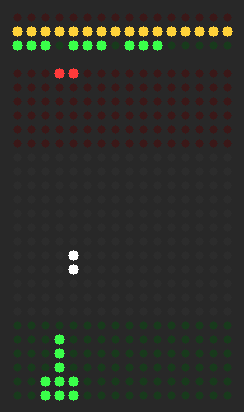
\includegraphics[width=\linewidth]{figures/phase1_1.png}\\[-2pt]
{\scriptsize\color{grey}}
\end{minipage}\hspace{4pt}%
\caption{What world.h draws or uses.}
\end{figure}

{\footnotesize\begin{longtable}{|>{\raggedright\arraybackslash}p{5.82cm}|>{\raggedright\arraybackslash}p{10.68cm}|}
\hline\rowcolor{accent}\textbf{\color{white}Function} & \textbf{\color{white}What it does}\\\hline\endhead
playerShip() & The table entry (speed, fire rate, ammo ...) of the ship in use.\\\hline
\rowcolor{rowshade}shipPixel(int8\_t x, int8\_t y) & True if the player's ship has a lit pixel at screen position (x, y): exact hits.\\\hline
addScore(uint16\_t points) & Adds points to the score, which stops at 9999 (four digits fit on the screen).\\\hline
\rowcolor{rowshade}playerShotCount() & Counts the player's bullets in the air (at most MAX\_PLAYER\_SHOTS).\\\hline
newShot(int8\_t x, int8\_t y, uint8\_t kind, uint16\_t stepMs) & Puts a new bullet or mine in a free slot of the shot pool and returns it, or NULL when all slots are in use.\\\hline
\rowcolor{rowshade}enemyShot(int8\_t x, int8\_t y, int8\_t dx, uint8\_t sideEvery, uint8\_t stepMs) & Fires an enemy bullet: straight down, or with dx = -1 / 1 one step sideways every sideEvery rows (spread shots).\\\hline
aimedShot(int8\_t x, int8\_t y, uint8\_t stepMs) & A shot that heads for the player: it steps sideways once every few rows.\\\hline
\rowcolor{rowshade}infoOf(const Enemy\& e) & The table entry (sprite, size, health, points, speed) of an enemy's type.\\\hline
fireDelay(uint16\_t ms) & Scales an enemy fire interval by the difficulty (EASY slower, HARD faster).\\\hline
\rowcolor{rowshade}spawnEnemy(uint8\_t type, int8\_t x, int8\_t y) & Puts a new enemy or rock of a type at (x, y) in a free slot and returns it, or NULL when all slots are in use.\\\hline
enemiesAlive() & Counts the enemies and rocks on the screen.\\\hline
\rowcolor{rowshade}spawnPickup(uint8\_t type, int8\_t x, int8\_t y) & Drops a pickup (ammo crate or extra life) at (x, y) if a slot is free.\\\hline
pickupAlive(uint8\_t type) & True if a pickup of this type is on the screen.\\\hline
\rowcolor{rowshade}explode(int8\_t cx, int8\_t cy, uint8\_t count, uint8\_t speed) & Starts an explosion: up to \texttt{count} pixels fly out from (cx, cy) at random speeds.\\\hline
bossSprite() & The picture of the current boss (the VOID KING has one per form).\\\hline
\rowcolor{rowshade}shake(uint8\_t frames) & Shakes the screen for some pictures (a longer shake already running is not cut short).\\\hline
worldClear() & Empties the game screen: no shots, enemies, pickups, explosion pixels or boss.\\\hline
\end{longtable}}

\subsubsection*{Source code}
\phantomsection\addcontentsline{toc}{subsubsection}{Source code}
\begin{lstlisting}[language=Arduino]
/*
 * world.h -- everything that lives on the game screen: the player, bullets, enemies and
 * rocks, pickups, explosion particles and the boss.
 *
 * Only fixed-size arrays (no malloc): the Mega has 8 KB of RAM and nothing may run out in
 * the middle of a game. Positions are in LED pixels, (0,0) = top-left of the game screen.
 * All timing uses gameMs, a clock that advances one frame at a time and stops on pause.
 */
#pragma once
#include "config.h"
#include "display.h"
#include "sound.h"
#include "tunes.h"
#include "art.h"
#include "storage.h"

uint32_t gameMs = 0;
const int8_t PLAYER_MIN_Y = 9, PLAYER_MAX_Y = SCREEN_H - 3;

// ================================================================= the three ships
struct ShipInfo {
  const char* name;                      // in flash
  const uint16_t* sprite;
  uint8_t moveMs;                        // ms per pixel while gliding
  uint16_t fireMs;                       // ms between shots while R is held
  uint8_t ammoMax;
  bool twin;                             // two guns: two bullets, two ammo per shot
  uint8_t speedLevel, ammoLevel, fireLevel;   // 1..3, shown in the hangar
};
const char NAME_BOLT[] PROGMEM = "BOLT";
const char NAME_DART[] PROGMEM = "DART";
const char NAME_TWIN[] PROGMEM = "TWIN";
const ShipInfo SHIPS[3] = {
  {NAME_BOLT, SHIP_BOLT, 70, 200, 60, false, 2, 2, 2},
  {NAME_DART, SHIP_DART, 45, 220, 40, false, 3, 1, 2},
  {NAME_TWIN, SHIP_TWIN, 95, 260, 80, true, 1, 3, 3},
};

// ================================================================= player
struct Player {
  int8_t x, y;                           // top-left of the 3 x 3 ship
  uint8_t ship, lives, ammo;
  uint16_t score;
  bool firing;                           // R was pressed and no move key cancelled it
  uint8_t burst;                         // shots since R was pressed
  char moveKey;                          // move key that is held (0 = none)
  bool gliding;                          // the key was held long enough to glide
  uint32_t nextShot, nextMove, shieldUntil;
  bool lowAmmoWarned;
};
Player player;
bool testShield = false;                 // test hook: the player can't be hit
bool autopilot = false;                  // test hook: the game plays itself

// The table entry (speed, fire rate, ammo ...) of the ship in use.
const ShipInfo& playerShip() {
  return SHIPS[player.ship];
}

// True if the player's ship has a lit pixel at screen position (x, y): exact hits.
bool shipPixel(int8_t x, int8_t y) {
  int8_t c = x - player.x, r = y - player.y;
  if (c < 0 || c > 2 || r < 0 || r > 2) return false;
  return pgm_read_word(playerShip().sprite + r) & (0x8000u >> c);
}

// Adds points to the score, which stops at 9999 (four digits fit on the screen).
void addScore(uint16_t points) {
  player.score = (player.score + points > 9999) ? 9999 : player.score + points;
}

// ================================================================= shots (player and enemy)
enum ShotKind : uint8_t { SHOT_PLAYER, SHOT_ENEMY, SHOT_MINE };
struct Shot {
  int8_t x, y, dx;                       // dx: sideways step (-1, 0, 1)
  uint8_t sideEvery, sideCount;          // sideways step every n down steps
  uint16_t stepMs;                       // ms per pixel
  uint8_t kind;
  uint32_t next;
  bool alive;
};
const uint8_t MAX_SHOTS = 28, MAX_PLAYER_SHOTS = 6;
Shot shots[MAX_SHOTS];

// Counts the player's bullets in the air (at most MAX_PLAYER_SHOTS).
uint8_t playerShotCount() {
  uint8_t n = 0;
  for (uint8_t i = 0; i < MAX_SHOTS; i++)
    if (shots[i].alive && shots[i].kind == SHOT_PLAYER) n++;
  return n;
}

// Puts a new bullet or mine in a free slot of the shot pool and returns it, or NULL when
// all slots are in use.
Shot* newShot(int8_t x, int8_t y, uint8_t kind, uint16_t stepMs) {
  for (uint8_t i = 0; i < MAX_SHOTS; i++) {
    Shot& s = shots[i];
    if (s.alive) continue;
    s = {x, y, 0, 1, 0, stepMs, kind, gameMs + stepMs, true};
    return &s;
  }
  return NULL;                           // pool full: the shot is simply not fired
}

// Fires an enemy bullet: straight down, or with dx = -1 / 1 one step sideways every
// sideEvery rows (spread shots).
void enemyShot(int8_t x, int8_t y, int8_t dx, uint8_t sideEvery, uint8_t stepMs) {
  Shot* s = newShot(x, y, SHOT_ENEMY, stepMs);
  if (s) {
    s->dx = dx;
    s->sideEvery = sideEvery;
  }
}

// A shot that heads for the player: it steps sideways once every few rows.
void aimedShot(int8_t x, int8_t y, uint8_t stepMs) {
  int8_t cols = (player.x + 1) - x, rows = player.y - y;
  if (rows < 1) rows = 1;
  int8_t dx = (cols > 0) - (cols < 0);
  uint8_t every = cols ? constrain(rows / abs(cols), 1, 6) : 1;
  enemyShot(x, y, dx, every, stepMs);
}

// ================================================================= enemies and rocks
enum EnemyType : uint8_t { EN_DRONE, EN_WEAVER, EN_MINER, EN_CRUISER, EN_ROCK_S, EN_ROCK_B };
struct EnemyInfo {
  const uint16_t* sprite;
  uint8_t w, h, hp;
  uint8_t score;
  uint16_t stepMs;                       // ms per pixel of its main movement
};
const EnemyInfo ENEMY_INFO[6] = {
  {ENEMY_DRONE, 3, 2, 1, 10, 450},
  {ENEMY_WEAVER, 3, 2, 1, 15, 600},
  {ENEMY_MINER, 3, 2, 2, 20, 280},
  {ENEMY_CRUISER, 5, 3, 5, 40, 500},
  {ROCK_SMALL, 3, 3, 1, 5, 360},
  {ROCK_BIG, 4, 3, 2, 10, 520},
};
struct Enemy {
  int8_t x, y, dir;
  uint8_t type, hp, flash, steps;
  uint32_t nextMove, nextSide, nextShot;
  bool alive;
};
const uint8_t MAX_ENEMIES = 16;
Enemy enemies[MAX_ENEMIES];

// The table entry (sprite, size, health, points, speed) of an enemy's type.
const EnemyInfo& infoOf(const Enemy& e) {
  return ENEMY_INFO[e.type];
}

// Scales an enemy fire interval by the difficulty (EASY slower, HARD faster).
uint16_t fireDelay(uint16_t ms) {
  return (uint32_t)ms * DIFF_FIRE_SCALE[settings.difficulty] / 100;
}

// Puts a new enemy or rock of a type at (x, y) in a free slot and returns it, or NULL
// when all slots are in use.
Enemy* spawnEnemy(uint8_t type, int8_t x, int8_t y) {
  for (uint8_t i = 0; i < MAX_ENEMIES; i++) {
    Enemy& e = enemies[i];
    if (e.alive) continue;
    const EnemyInfo& info = ENEMY_INFO[type];
    e = {x, y, 1, type, info.hp, 0, 0, gameMs + info.stepMs, gameMs + 300,
         gameMs + fireDelay(1200 + random(1500)), true};
    return &e;
  }
  return NULL;
}

// Counts the enemies and rocks on the screen.
uint8_t enemiesAlive() {
  uint8_t n = 0;
  for (uint8_t i = 0; i < MAX_ENEMIES; i++) n += enemies[i].alive;
  return n;
}

// ================================================================= pickups
enum PickupType : uint8_t { PK_AMMO, PK_LIFE };
struct Pickup {
  int8_t x, y;
  uint8_t type;
  uint32_t next;
  bool alive;
};
const uint8_t MAX_PICKUPS = 4;
Pickup pickups[MAX_PICKUPS];

// Drops a pickup (ammo crate or extra life) at (x, y) if a slot is free.
void spawnPickup(uint8_t type, int8_t x, int8_t y) {
  for (uint8_t i = 0; i < MAX_PICKUPS; i++)
    if (!pickups[i].alive) {
      pickups[i] = {(int8_t)constrain(x, 0, SCREEN_W - 3), y, type, gameMs + 350, true};
      return;
    }
}

// True if a pickup of this type is on the screen.
bool pickupAlive(uint8_t type) {
  for (uint8_t i = 0; i < MAX_PICKUPS; i++)
    if (pickups[i].alive && pickups[i].type == type) return true;
  return false;
}

// ================================================================= explosion particles
// Only the boss and the player's ship explode into flying pixels; ordinary enemies just
// vanish, so the small screen does not fill up with debris that looks like bullets.
struct Particle {
  int16_t x16, y16;                      // position in 1/16 pixel
  int8_t vx, vy;                         // speed in 1/16 pixel per frame
  uint8_t life;                          // frames left
};
const uint8_t MAX_PARTICLES = 40;
Particle particles[MAX_PARTICLES];

// Starts an explosion: up to `count` pixels fly out from (cx, cy) at random speeds.
void explode(int8_t cx, int8_t cy, uint8_t count, uint8_t speed) {
  for (uint8_t i = 0; i < MAX_PARTICLES && count; i++) {
    Particle& p = particles[i];
    if (p.life) continue;
    p = {(int16_t)(cx * 16 + 8), (int16_t)(cy * 16 + 8), (int8_t)random(-speed, speed + 1),
         (int8_t)random(-speed, speed + 1), (uint8_t)random(8, 18)};
    count--;
  }
}

// ================================================================= boss
enum BossKind : uint8_t { BOSS_KIND_WARDEN, BOSS_KIND_HUNTER, BOSS_KIND_KING };
struct Boss {
  bool alive;
  uint8_t kind, w, h, flash, form, mode;
  int8_t x, y, dir, targetX;
  int16_t hp, maxHp;
  uint32_t nextMove, nextShot, nextAction, modeUntil;
  uint8_t burst;
};
Boss boss;

// The picture of the current boss (the VOID KING has one per form).
const uint16_t* bossSprite() {
  if (boss.kind == BOSS_KIND_WARDEN) return BOSS_WARDEN;
  if (boss.kind == BOSS_KIND_HUNTER) return BOSS_HUNTER;
  return boss.form ? BOSS_KING_ANGRY : BOSS_KING;
}

// ================================================================= helpers
// True when two boxes overlap (the ship against enemies, rocks, the boss, pickups).
bool boxesTouch(int8_t ax, int8_t ay, uint8_t aw, uint8_t ah,
                int8_t bx, int8_t by, uint8_t bw, uint8_t bh) {
  return ax < bx + bw && bx < ax + aw && ay < by + bh && by < ay + ah;
}

uint8_t shakeFrames = 0;
// Shakes the screen for some pictures (a longer shake already running is not cut short).
void shake(uint8_t frames) {
  if (frames > shakeFrames) shakeFrames = frames;
}

// Empties the game screen: no shots, enemies, pickups, explosion pixels or boss.
void worldClear() {
  for (uint8_t i = 0; i < MAX_SHOTS; i++) shots[i].alive = false;
  for (uint8_t i = 0; i < MAX_ENEMIES; i++) enemies[i].alive = false;
  for (uint8_t i = 0; i < MAX_PICKUPS; i++) pickups[i].alive = false;
  for (uint8_t i = 0; i < MAX_PARTICLES; i++) particles[i].life = 0;
  boss.alive = false;
}
\end{lstlisting}

\clearpage
\subsection*{4.15 player.h – The player's ship}
\phantomsection\addcontentsline{toc}{subsection}{4.15 player.h – The player's ship}
The key rules for moving and firing (tap, hold, auto-fire, newest key wins), ammo and the low-ammo warning, getting hit (a life, explosion, shake, shield) and drawing the ship.

\begin{figure}[H]\centering
\begin{minipage}[t]{3.20cm}\centering
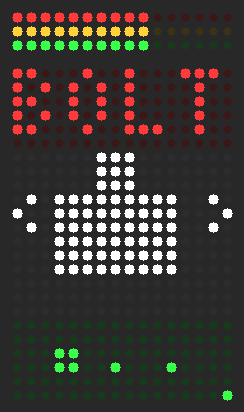
\includegraphics[width=\linewidth]{figures/hangar_bolt.png}\\[-2pt]
{\scriptsize\color{grey}}
\end{minipage}\hspace{4pt}%
\begin{minipage}[t]{3.20cm}\centering
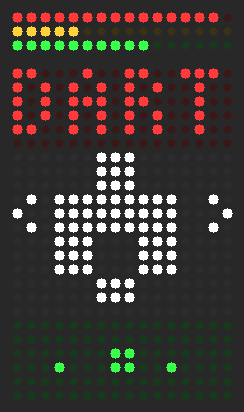
\includegraphics[width=\linewidth]{figures/hangar_dart.png}\\[-2pt]
{\scriptsize\color{grey}}
\end{minipage}\hspace{4pt}%
\begin{minipage}[t]{3.20cm}\centering
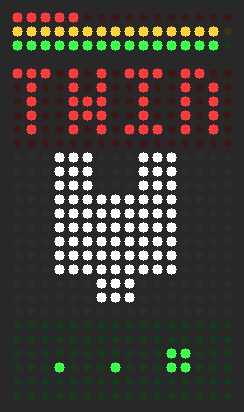
\includegraphics[width=\linewidth]{figures/hangar_twin.png}\\[-2pt]
{\scriptsize\color{grey}}
\end{minipage}\hspace{4pt}%
\caption{What player.h draws or uses.}
\end{figure}

\par\noindent\begin{minipage}{\linewidth}\centering\footnotesize
\begin{tabular}{|>{\raggedright\arraybackslash}p{5.82cm}|>{\raggedright\arraybackslash}p{10.68cm}|}
\hline\rowcolor{accent}\textbf{\color{white}Function} & \textbf{\color{white}What it does}\\\hline
playerStart(bool newGame) & Gets the ship ready: bottom centre, full ammo, not firing. newGame = also the ship from the hangar, the lives of the difficulty and score 0 (a new phase keeps those).\\\hline
\rowcolor{rowshade}playerShielded() & True while the ship can't be hit (2 s after a hit, or the test hook !i).\\\hline
movePlayer(char key) & Moves the ship one pixel in the direction of a move key, staying on the screen and in rows 9-23.\\\hline
\rowcolor{rowshade}playerFire() & Fires one shot (TWIN: two bullets) if there is ammo and a free bullet slot. Plays the shot sound (a chirp when auto-fire starts) and warns once when ammo gets low.\\\hline
playerKeys() & Keys: called once per picture (key presses are counted per picture).\\\hline
\rowcolor{rowshade}playerStep() & Movement and fire: called once per game step (20 ms of game time).\\\hline
playerHit(const \_\_FlashStringHelper* cause) & The ship is hit (unless shielded): one life less, 2 s shield, explosion, shake and sound. cause says what hit it, for the Serial log, e.g. F("shot").\\\hline
\rowcolor{rowshade}drawPlayer(uint16\_t frameNo) & Draws the ship and its engine flame; it blinks while shielded, and its nose blinks during auto-fire.\\\hline
\end{tabular}
\end{minipage}\par\medskip

\subsubsection*{Source code}
\phantomsection\addcontentsline{toc}{subsubsection}{Source code}
\begin{lstlisting}[language=Arduino]
/*
 * player.h -- the player's ship: moving, firing, ammo and lives.
 *
 * Key rules (agreed in the design):
 *   move   tap = one pixel; hold = after a short delay the ship glides at its speed
 *   fire   press R = one bullet; keep holding = auto-fire (a chirp, the nose blinks);
 *          release R = stop
 *   The newest key wins: a move key stops the fire (press R again to fire again), and
 *   while R is held the ship does not glide.
 * Every shot costs ammo (TWIN: two bullets, two ammo). At LOW_AMMO a warning beeps and
 * the yellow bar blinks. A hit costs a life and gives two seconds of blinking shield.
 */
#pragma once
#include "world.h"
#include "input.h"

const char MOVE_KEYS[4] = {KEY_UP, KEY_LEFT, KEY_DOWN, KEY_RIGHT};

// Gets the ship ready: bottom centre, full ammo, not firing. newGame = also the ship from
// the hangar, the lives of the difficulty and score 0 (a new phase keeps those).
void playerStart(bool newGame) {
  if (newGame) {
    player.ship = settings.ship;
    player.lives = DIFF_LIVES[settings.difficulty];
    player.score = 0;
  }
  player.x = (SCREEN_W - 3) / 2;
  player.y = SCREEN_H - 4;
  player.ammo = playerShip().ammoMax;    // every phase starts with a full magazine
  player.firing = false;
  player.moveKey = 0;
  player.shieldUntil = 0;
  player.lowAmmoWarned = false;
}

// True while the ship can't be hit (2 s after a hit, or the test hook !i).
bool playerShielded() {
  return testShield || gameMs < player.shieldUntil;
}

// Moves the ship one pixel in the direction of a move key, staying on the screen and in
// rows 9-23.
void movePlayer(char key) {
  int8_t dx = (key == KEY_RIGHT) - (key == KEY_LEFT);
  int8_t dy = (key == KEY_DOWN) - (key == KEY_UP);
  player.x = constrain(player.x + dx, 0, SCREEN_W - 3);
  player.y = constrain(player.y + dy, PLAYER_MIN_Y, PLAYER_MAX_Y);
}

// Fires one shot (TWIN: two bullets) if there is ammo and a free bullet slot. Plays the
// shot sound (a chirp when auto-fire starts) and warns once when ammo gets low.
void playerFire() {
  const ShipInfo& ship = playerShip();
  uint8_t bullets = (ship.twin && player.ammo >= 2) ? 2 : 1;
  if (player.ammo == 0) {
    soundSfx(SFX(SFX_EMPTY), 2);
    player.nextShot = gameMs + ship.fireMs;
    return;
  }
  if (playerShotCount() + bullets > MAX_PLAYER_SHOTS) return;   // try again next step
  if (bullets == 2) {
    newShot(player.x, player.y - 1, SHOT_PLAYER, PLAYER_SHOT_MS);
    newShot(player.x + 2, player.y - 1, SHOT_PLAYER, PLAYER_SHOT_MS);
  } else {
    newShot(player.x + 1, player.y - 1, SHOT_PLAYER, PLAYER_SHOT_MS);
  }
  player.ammo -= bullets;
  player.nextShot = gameMs + ship.fireMs;
  if (++player.burst == 2) soundSfx(SFX(SFX_CHIRP), 2);   // auto-fire has started
  else soundSfx(SFX(SFX_SHOT), 1);
  if (player.ammo <= LOW_AMMO && !player.lowAmmoWarned) {
    player.lowAmmoWarned = true;
    soundSfx(SFX(SFX_LOW_AMMO), 4);
  }
}

// Keys: called once per picture (key presses are counted per picture).
void playerKeys() {
  if (autopilot) return;
  for (uint8_t i = 0; i < 4; i++)
    if (keyPressed(MOVE_KEYS[i])) {      // newest move key takes over and stops the fire
      player.moveKey = MOVE_KEYS[i];
      player.gliding = false;
      player.nextMove = gameMs;          // first pixel right away
      player.firing = false;
    }
  if (keyPressed(KEY_FIRE)) {
    player.firing = true;
    player.burst = 0;
    player.nextShot = gameMs;            // first bullet right away
  }
  if (player.moveKey && !keyHeld(player.moveKey)) {   // let go: another held move key?
    player.moveKey = 0;
    for (uint8_t i = 0; i < 4; i++)
      if (keyHeld(MOVE_KEYS[i])) {
        player.moveKey = MOVE_KEYS[i];
        player.gliding = true;
        player.nextMove = gameMs + playerShip().moveMs;
      }
  }
}

// Movement and fire: called once per game step (20 ms of game time).
void playerStep() {
  if (player.lives == 0) return;
  if (player.firing) {
    if (!autopilot && !keyHeld(KEY_FIRE)) player.firing = false;   // R released
    else if (gameMs >= player.nextShot) playerFire();
  }
  if (!player.firing && player.moveKey && gameMs >= player.nextMove) {
    movePlayer(player.moveKey);
    player.nextMove = gameMs + (player.gliding ? playerShip().moveMs : MOVE_REPEAT_DELAY);
    player.gliding = true;
  }
}

// The ship is hit (unless shielded): one life less, 2 s shield, explosion, shake and sound.
// cause says what hit it, for the Serial log, e.g. F("shot").
void playerHit(const __FlashStringHelper* cause) {
  if (playerShielded() || player.lives == 0) return;
  player.lives--;
  player.shieldUntil = gameMs + HIT_SHIELD_MS;
  player.firing = false;
  explode(player.x + 1, player.y + 1, 12, 14);
  shake(12);
  soundSfx(SFX(SFX_PLAYER_HIT), 6);
  Serial.print(F("[VR] hit by "));
  Serial.print(cause);
  Serial.print(F(", lives "));
  Serial.println(player.lives);
}

// Draws the ship and its engine flame; it blinks while shielded, and its nose blinks
// during auto-fire.
void drawPlayer(uint16_t frameNo) {
  if (player.lives == 0) return;
  if (gameMs < player.shieldUntil && (frameNo & 8)) return;    // blinks while shielded
  const uint16_t* sprite = playerShip().sprite;
  drawBitmap(player.x, player.y, sprite, 3, 3, true);
  if (player.firing && player.burst >= 2 && (frameNo & 8))      // auto-fire: the nose blinks
    drawBitmap(player.x, player.y, sprite, 3, 1, false);
  if (frameNo & 1) setPixel(player.x + 1, player.y + 3, true);  // engine flame
}
\end{lstlisting}

\clearpage
\subsection*{4.16 enemies.h – Enemies and rocks}
\phantomsection\addcontentsline{toc}{subsection}{4.16 enemies.h – Enemies and rocks}
How each enemy type moves and shoots, and the rule that keeps them apart: a move may not bring an enemy closer than one empty pixel to another one, so it steps aside, turns or waits. New enemies take the nearest free column.

\begin{figure}[H]\centering
\begin{minipage}[t]{2.80cm}\centering

\includegraphics[width=\linewidth]{figures/sprite_enemy_drone.png}\\[-2pt]
{\scriptsize\color{grey}}
\end{minipage}\hspace{4pt}%
\begin{minipage}[t]{2.80cm}\centering

\includegraphics[width=\linewidth]{figures/sprite_enemy_weaver.png}\\[-2pt]
{\scriptsize\color{grey}}
\end{minipage}\hspace{4pt}%
\begin{minipage}[t]{2.80cm}\centering

\includegraphics[width=\linewidth]{figures/sprite_enemy_miner.png}\\[-2pt]
{\scriptsize\color{grey}}
\end{minipage}\hspace{4pt}%
\begin{minipage}[t]{2.80cm}\centering

\includegraphics[width=\linewidth]{figures/sprite_rock_small.png}\\[-2pt]
{\scriptsize\color{grey}}
\end{minipage}\hspace{4pt}%
\begin{minipage}[t]{2.80cm}\centering

\includegraphics[width=\linewidth]{figures/sprite_rock_big.png}\\[-2pt]
{\scriptsize\color{grey}}
\end{minipage}\hspace{4pt}%
\caption{What enemies.h draws or uses.}
\end{figure}

\par\noindent\begin{minipage}{\linewidth}\centering\footnotesize
\begin{tabular}{|>{\raggedright\arraybackslash}p{5.82cm}|>{\raggedright\arraybackslash}p{10.68cm}|}
\hline\rowcolor{accent}\textbf{\color{white}Function} & \textbf{\color{white}What it does}\\\hline
touchesOther(const Enemy\& e, int8\_t x, int8\_t y, uint8\_t gap) & True if enemy e, placed at (x, y), would touch another enemy: with gap = 1 also when they are only side by side with no empty pixel between them.\\\hline
\rowcolor{rowshade}canMoveTo(const Enemy\& e, int8\_t x, int8\_t y) & True if enemy e may move to (x, y). On 16 x 24 LEDs two enemies on the same pixels merge into one unreadable blob, so a move may not bring it closer than one empty pixel to another enemy (a move is still allowed if they were already that close, so two enemies side by side can't block each other forever).\\\hline
moveDown(Enemy\& e) & Moves an enemy one pixel down. If something is in the way it steps aside instead (its own direction first), or waits for this step.\\\hline
\rowcolor{rowshade}moveSide(Enemy\& e) & Moves an enemy one pixel sideways in its direction; if something is in the way (or the screen edge: only miners fly in and out at the sides) it turns around instead. Returns true if it moved.\\\hline
spawnFromTable(uint8\_t type, int8\_t x) & Puts an enemy on the screen just above the top (miners come in from the side).\\\hline
\rowcolor{rowshade}updateEnemy(Enemy\& e) & Moves one enemy or rock for one game step and lets it shoot; each type has its own pattern (see the list at the top). Anything that leaves at the bottom is removed.\\\hline
updateEnemies() & Updates every enemy and rock that is alive (once per game step).\\\hline
\rowcolor{rowshade}drawEnemies() & Draws every enemy and rock; one that was just hit is hidden for a moment.\\\hline
\end{tabular}
\end{minipage}\par\medskip

\subsubsection*{Source code}
\phantomsection\addcontentsline{toc}{subsubsection}{Source code}
\begin{lstlisting}[language=Arduino]
/*
 * enemies.h -- how each enemy and rock moves and shoots. Every one moves slowly (the
 * player is always faster); each type has its own shot:
 *   drone     sinks, shoots straight down
 *   weaver    sinks while zig-zagging, shoots straight down now and then
 *   miner     crosses the top of the screen and drops mines
 *   cruiser   stops near the top, slides sideways and fires shots aimed at the player
 *   rocks     fall and drift; a big rock breaks into two small ones
 */
#pragma once
#include "world.h"

const int8_t ENEMY_FIRE_MAX_Y = 9;

// True if enemy e, placed at (x, y), would touch another enemy: with gap = 1 also when they
// are only side by side with no empty pixel between them.
bool touchesOther(const Enemy& e, int8_t x, int8_t y, uint8_t gap) {
  const EnemyInfo& info = infoOf(e);
  for (uint8_t i = 0; i < MAX_ENEMIES; i++) {
    const Enemy& o = enemies[i];
    if (!o.alive || &o == &e) continue;
    const EnemyInfo& oi = infoOf(o);
    if (boxesTouch(x - gap, y - gap, info.w + 2 * gap, info.h + 2 * gap, o.x, o.y, oi.w, oi.h))
      return true;
  }
  return false;
}

// True if enemy e may move to (x, y). On 16 x 24 LEDs two enemies on the same pixels merge
// into one unreadable blob, so a move may not bring it closer than one empty pixel to
// another enemy (a move is still allowed if they were already that close, so two enemies
// side by side can't block each other forever).
bool canMoveTo(const Enemy& e, int8_t x, int8_t y) {
  if (touchesOther(e, x, y, 0) && !touchesOther(e, e.x, e.y, 0)) return false;
  return !touchesOther(e, x, y, 1) || touchesOther(e, e.x, e.y, 1);
}

// Moves an enemy one pixel down. If something is in the way it steps aside instead (its
// own direction first), or waits for this step.
void moveDown(Enemy& e) {
  if (canMoveTo(e, e.x, e.y + 1)) { e.y++; return; }
  const int8_t maxX = SCREEN_W - infoOf(e).w;
  int8_t d = e.dir ? e.dir : 1;
  for (uint8_t i = 0; i < 2; i++, d = -d) {
    int8_t x = e.x + d;
    if (x >= 0 && x <= maxX && canMoveTo(e, x, e.y)) { e.x = x; return; }
  }
}

// Moves an enemy one pixel sideways in its direction; if something is in the way (or the
// screen edge: only miners fly in and out at the sides) it turns around instead. Returns
// true if it moved.
bool moveSide(Enemy& e) {
  int8_t x = e.x + e.dir;
  bool inside = e.type == EN_MINER || (x >= 0 && x <= SCREEN_W - infoOf(e).w);
  if (inside && canMoveTo(e, x, e.y)) { e.x = x; return true; }
  e.dir = -e.dir;
  return false;
}

// Puts an enemy on the screen just above the top (miners come in from the side).
void spawnFromTable(uint8_t type, int8_t x) {
  const EnemyInfo& info = ENEMY_INFO[type];
  if (type == EN_MINER) {
    bool fromLeft = x < SCREEN_W / 2;
    Enemy* e = spawnEnemy(type, fromLeft ? -3 : SCREEN_W, 1 + random(3));
    if (!e) return;
    e->dir = fromLeft ? 1 : -1;
    while (e->x > -20 && e->x < SCREEN_W + 20 && touchesOther(*e, e->x, e->y, 1))
      e->x -= e->dir;                    // another one is there: queue up further outside
    return;
  }
  Enemy* e = spawnEnemy(type, constrain(x, 0, SCREEN_W - info.w), -info.h);
  if (!e) return;
  // Something is already entering there: take the nearest free column (+1, -1, +2, -2 ...),
  // and if the whole row is busy, queue up higher above the screen.
  for (int8_t d = 1; d < 2 * SCREEN_W && touchesOther(*e, e->x, e->y, 1); d++) {
    int8_t tryX = e->x + ((d & 1) ? (d + 1) / 2 : -d / 2);
    if (tryX >= 0 && tryX <= SCREEN_W - info.w && !touchesOther(*e, tryX, e->y, 1)) e->x = tryX;
  }
  while (e->y > -20 && touchesOther(*e, e->x, e->y, 1)) e->y--;
  if (type == EN_ROCK_S || type == EN_ROCK_B) e->dir = random(3) - 1;   // drift
}

// Moves one enemy or rock for one game step and lets it shoot; each type has its own
// pattern (see the list at the top). Anything that leaves at the bottom is removed.
void updateEnemy(Enemy& e) {
  const EnemyInfo& info = infoOf(e);
  // Enemies only shoot from the upper part of the screen: a bullet fired right next to
  // the ship could not be dodged. The ship may fly up to row 9 too, so a bullet must also
  // start at least 3 rows above it.
  bool canShoot = e.y >= 0 && e.y <= ENEMY_FIRE_MAX_Y && e.y + info.h + 3 <= player.y;
  switch (e.type) {
    case EN_DRONE:
      if (gameMs >= e.nextMove) { moveDown(e); e.nextMove += info.stepMs; }
      if (gameMs >= e.nextShot) {
        if (canShoot) enemyShot(e.x + 1, e.y + 2, 0, 1, 110);
        e.nextShot = gameMs + fireDelay(2600 + random(1800));
      }
      break;

    case EN_WEAVER:
      if (gameMs >= e.nextMove) { moveDown(e); e.nextMove += info.stepMs; }
      if (gameMs >= e.nextSide) {              // zig-zag: three steps one way, then back
        if (!moveSide(e)) e.steps = 0;         // blocked: zig-zags back early
        else if (++e.steps >= 3 || e.x <= 0 || e.x >= SCREEN_W - info.w) {
          e.dir = -e.dir;
          e.steps = 0;
        }
        e.nextSide = gameMs + 220;
      }
      if (gameMs >= e.nextShot) {
        if (canShoot) enemyShot(e.x + 1, e.y + 2, 0, 1, 100);
        e.nextShot = gameMs + fireDelay(4000 + random(2000));
      }
      break;

    case EN_MINER:
      if (gameMs >= e.nextMove) { moveSide(e); e.nextMove += info.stepMs; }   // blocked: turns back
      if (gameMs >= e.nextShot) {
        if (e.x >= 0 && e.x <= SCREEN_W - info.w) newShot(e.x + 1, e.y + 2, SHOT_MINE, 300);
        e.nextShot = gameMs + fireDelay(1300);
      }
      if ((e.dir > 0 && e.x > SCREEN_W) || (e.dir < 0 && e.x < -info.w)) e.alive = false;
      break;

    case EN_CRUISER:
      if (e.y < 3) {
        if (gameMs >= e.nextMove) { moveDown(e); e.nextMove += info.stepMs; }
      } else if (gameMs >= e.nextSide) {
        if (moveSide(e) && (e.x <= 0 || e.x >= SCREEN_W - info.w)) e.dir = -e.dir;
        e.nextSide = gameMs + 650;
      }
      if (gameMs >= e.nextShot) {
        if (e.y >= 0) aimedShot(e.x + 2, e.y + 3, 100);
        e.nextShot = gameMs + fireDelay(1800);
      }
      break;

    default:                                   // rocks
      if (gameMs >= e.nextMove) { moveDown(e); e.nextMove += info.stepMs; }
      if (e.dir && gameMs >= e.nextSide) {
        if (e.x + e.dir < 0 || e.x + e.dir > SCREEN_W - info.w) e.dir = -e.dir;   // edge
        else moveSide(e);
        e.nextSide = gameMs + 1400;
      }
      break;
  }
  if (e.y >= SCREEN_H) e.alive = false;        // left the screen at the bottom
  if (e.flash) e.flash--;
}

// Updates every enemy and rock that is alive (once per game step).
void updateEnemies() {
  for (uint8_t i = 0; i < MAX_ENEMIES; i++)
    if (enemies[i].alive) updateEnemy(enemies[i]);
}

// Draws every enemy and rock; one that was just hit is hidden for a moment.
void drawEnemies() {
  for (uint8_t i = 0; i < MAX_ENEMIES; i++) {
    const Enemy& e = enemies[i];
    if (!e.alive || e.flash) continue;   // a hit enemy disappears for a moment (120 ms)
    const EnemyInfo& info = infoOf(e);
    drawBitmap(e.x, e.y, info.sprite, info.w, info.h, true);
  }
}
\end{lstlisting}

\clearpage
\subsection*{4.17 levels.h – The three phases}
\phantomsection\addcontentsline{toc}{subsection}{4.17 levels.h – The three phases}
The spawn list of each phase (wait, what, where), its enemy limit, its name, its song and its boss. The lists are stored in flash.

\begin{figure}[H]\centering
\begin{minipage}[t]{3.20cm}\centering
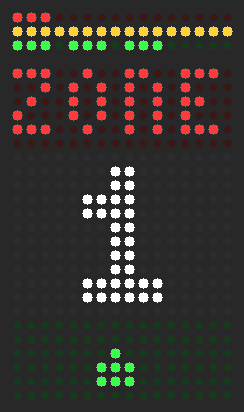
\includegraphics[width=\linewidth]{figures/zone1.png}\\[-2pt]
{\scriptsize\color{grey}}
\end{minipage}\hspace{4pt}%
\begin{minipage}[t]{3.20cm}\centering
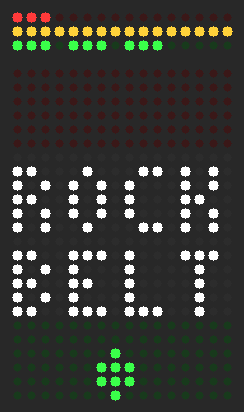
\includegraphics[width=\linewidth]{figures/rockbelt.png}\\[-2pt]
{\scriptsize\color{grey}}
\end{minipage}\hspace{4pt}%
\begin{minipage}[t]{3.20cm}\centering
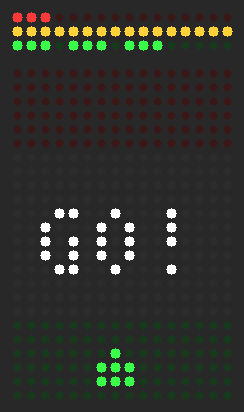
\includegraphics[width=\linewidth]{figures/go.png}\\[-2pt]
{\scriptsize\color{grey}}
\end{minipage}\hspace{4pt}%
\caption{What levels.h draws or uses.}
\end{figure}

\par\noindent\begin{minipage}{\linewidth}\centering\footnotesize
\begin{tabular}{|>{\raggedright\arraybackslash}p{5.82cm}|>{\raggedright\arraybackslash}p{10.68cm}|}
\hline\rowcolor{accent}\textbf{\color{white}Function} & \textbf{\color{white}What it does}\\\hline
spawnAt(uint8\_t phase, uint8\_t i) & Copies entry i of a phase's spawn list from flash into RAM.\\\hline
\end{tabular}
\end{minipage}\par\medskip

\subsubsection*{Source code}
\phantomsection\addcontentsline{toc}{subsubsection}{Source code}
\begin{lstlisting}[language=Arduino]
/*
 * levels.h -- the three phases. Each phase is a list of spawns: wait (in 0.1 s after the
 * previous spawn), what, and x. SP_CLEAR waits until the screen is empty; SP_AMMO and
 * SP_LIFE drop a pickup. After the last entry (and an empty screen) the boss comes.
 * The enemies are slow, so they would pile up: the list also waits while the phase's
 * maximum number of enemies is on the screen (that keeps 16 x 24 LEDs readable).
 */
#pragma once
#include "world.h"
#include "tunes.h"

struct Spawn { uint8_t wait, what; int8_t x; };
const uint8_t SP_AMMO = 10, SP_LIFE = 11, SP_CLEAR = 12;
#define DR EN_DRONE
#define WV EN_WEAVER
#define MN EN_MINER
#define CR EN_CRUISER
#define RS EN_ROCK_S
#define RB EN_ROCK_B

// ---- phase 1: Rock Belt (asteroids) -- drones and lots of rocks
const Spawn PHASE1[] PROGMEM = {
  {15, RS, 3}, {12, DR, 2}, {8, DR, 11}, {12, RB, 6}, {12, DR, 6},
  {0, DR, 10}, {12, RS, 12}, {10, SP_CLEAR, 0}, {5, SP_AMMO, 7},
  {10, DR, 1}, {5, DR, 6}, {5, DR, 11}, {14, RB, 3}, {12, DR, 4},
  {0, DR, 9}, {12, RS, 7}, {10, DR, 2}, {4, DR, 7}, {4, DR, 12},
  {12, RB, 0}, {10, SP_CLEAR, 0}, {5, SP_AMMO, 3},
  {8, DR, 0}, {3, DR, 4}, {3, DR, 8}, {3, DR, 12}, {14, RB, 6},
  {12, RS, 12}, {10, SP_CLEAR, 0},
};

// ---- phase 2: Deep Mist (a nebula) -- weavers and mine-layers
const Spawn PHASE2[] PROGMEM = {
  {15, WV, 3}, {10, WV, 10}, {14, MN, 0}, {12, DR, 6}, {10, WV, 1},
  {6, WV, 12}, {14, DR, 7}, {10, MN, 15}, {12, DR, 2}, {0, DR, 11},
  {12, SP_CLEAR, 0}, {5, SP_AMMO, 6},
  {10, WV, 5}, {4, WV, 9}, {12, MN, 0}, {8, MN, 15}, {14, RB, 6},
  {10, DR, 1}, {4, DR, 7}, {4, DR, 12}, {12, WV, 2}, {6, WV, 11},
  {10, RS, 4}, {12, SP_CLEAR, 0}, {5, SP_LIFE, 9},
  {10, MN, 0}, {6, WV, 6}, {6, WV, 9}, {10, MN, 15}, {10, DR, 3},
  {4, DR, 10}, {12, SP_CLEAR, 0}, {5, SP_AMMO, 4},
};

// ---- phase 3: The Void -- cruisers, everything else, and rock showers
const Spawn PHASE3[] PROGMEM = {
  {15, CR, 5}, {14, DR, 1}, {4, DR, 12}, {12, RS, 3}, {8, RS, 12},
  {14, WV, 6}, {12, SP_CLEAR, 0}, {5, SP_AMMO, 5},
  {10, CR, 1}, {16, CR, 10}, {10, RB, 6}, {8, RS, 14},
  {12, WV, 2}, {4, WV, 11}, {12, MN, 0}, {12, SP_CLEAR, 0}, {5, SP_AMMO, 9},
  {8, RS, 2}, {6, RS, 10}, {8, RB, 5},
  {12, DR, 0}, {3, DR, 5}, {3, DR, 10}, {10, CR, 5}, {12, WV, 1},
  {4, WV, 12}, {12, SP_CLEAR, 0}, {5, SP_LIFE, 7}, {5, SP_AMMO, 3},
};

#undef DR
#undef WV
#undef MN
#undef CR
#undef RS
#undef RB

struct PhaseInfo {
  const Spawn* spawns;
  uint8_t count;
  uint8_t maxEnemies;                    // at most this many on the screen at once
  const char* name1;                     // the phase name: two words of up to 4
  const char* name2;                     // letters (in flash), shown as a page
  const Track* song;
  uint8_t songTickMs;
  uint8_t boss;
};
const char NAME_ROCK[] PROGMEM = "ROCK";
const char NAME_BELT[] PROGMEM = "BELT";
const char NAME_DEEP[] PROGMEM = "DEEP";
const char NAME_MIST[] PROGMEM = "MIST";
const char NAME_THE[] PROGMEM = "THE";
const char NAME_VOID[] PROGMEM = "VOID";
const PhaseInfo PHASES[3] = {
  {PHASE1, sizeof(PHASE1) / sizeof(Spawn), 4, NAME_ROCK, NAME_BELT, SONG_PHASE1, SONG_PHASE1_TICK_MS, BOSS_KIND_WARDEN},
  {PHASE2, sizeof(PHASE2) / sizeof(Spawn), 5, NAME_DEEP, NAME_MIST, SONG_PHASE2, SONG_PHASE2_TICK_MS, BOSS_KIND_HUNTER},
  {PHASE3, sizeof(PHASE3) / sizeof(Spawn), 6, NAME_THE, NAME_VOID, SONG_PHASE3, SONG_PHASE3_TICK_MS, BOSS_KIND_KING},
};

// Copies entry i of a phase's spawn list from flash into RAM.
Spawn spawnAt(uint8_t phase, uint8_t i) {
  Spawn s;
  memcpy_P(&s, &PHASES[phase].spawns[i], sizeof(Spawn));
  return s;
}
\end{lstlisting}

\clearpage
\subsection*{4.18 boss.h – The bosses}
\phantomsection\addcontentsline{toc}{subsection}{4.18 boss.h – The bosses}
The behaviour of the WARDEN, the HUNTER (a small state machine: dash, aim, charge) and the VOID KING (two forms), their health and their drawing.

\begin{figure}[H]\centering
\begin{minipage}[t]{3.20cm}\centering
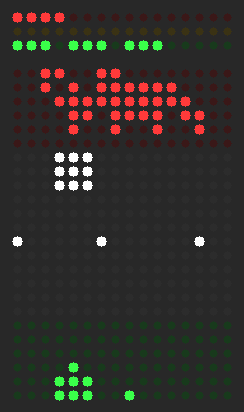
\includegraphics[width=\linewidth]{figures/warden_1.png}\\[-2pt]
{\scriptsize\color{grey}}
\end{minipage}\hspace{4pt}%
\begin{minipage}[t]{3.20cm}\centering
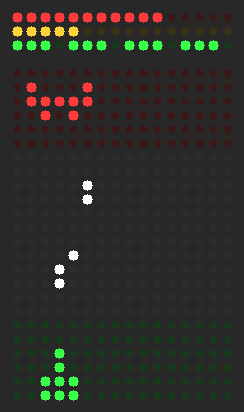
\includegraphics[width=\linewidth]{figures/hunter1.png}\\[-2pt]
{\scriptsize\color{grey}}
\end{minipage}\hspace{4pt}%
\begin{minipage}[t]{3.20cm}\centering
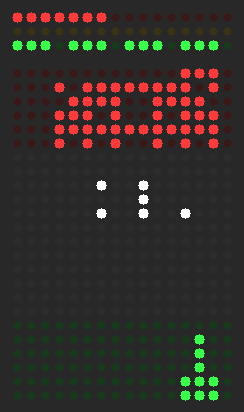
\includegraphics[width=\linewidth]{figures/king2.png}\\[-2pt]
{\scriptsize\color{grey}}
\end{minipage}\hspace{4pt}%
\caption{What boss.h draws or uses.}
\end{figure}

\par\noindent\begin{minipage}{\linewidth}\centering\footnotesize
\begin{tabular}{|>{\raggedright\arraybackslash}p{5.82cm}|>{\raggedright\arraybackslash}p{10.68cm}|}
\hline\rowcolor{accent}\textbf{\color{white}Function} & \textbf{\color{white}What it does}\\\hline
bossStart(uint8\_t kind) & Gets the boss of a phase ready: its size, its health (scaled by the difficulty), a start just above the screen so it slides in, and the times of its first shot and action.\\\hline
\rowcolor{rowshade}bossAngry() & True when the boss has lost half its health or more (it then attacks harder).\\\hline
bossSlide(uint16\_t ms) & Moves the boss one pixel sideways every \texttt{ms}, turning around at the screen edges.\\\hline
\rowcolor{rowshade}updateWarden() & WARDEN's turn: slides along the top, fires a 3-way spread (5-way when angry) and drops rocks every 7 seconds.\\\hline
updateHunter() & HUNTER's turn, a small state machine (boss.mode): FIGHT picks the next move, DASH flies fast to a random column, AIM fires a pair of aimed shots, CHARGE\_DOWN / CHARGE\_UP dives at the player and climbs back.\\\hline
\rowcolor{rowshade}updateKing() & VOID KING's turn. Below half health it changes form once (eye opens, roar, shake). Form 1: 5-way spread and calls in drones. Form 2: aimed triple volleys and rock rain.\\\hline
updateBoss() & Moves the boss for one game step: first it slides in from the top, then it runs the behaviour of its kind.\\\hline
\rowcolor{rowshade}drawBoss(uint16\_t frameNo) & Draws the boss; while boss.flash counts down it blinks (before a dive, at the form change and while it burns).\\\hline
\end{tabular}
\end{minipage}\par\medskip

\subsubsection*{Source code}
\phantomsection\addcontentsline{toc}{subsubsection}{Source code}
\begin{lstlisting}[language=Arduino]
/*
 * boss.h -- the three bosses (health is shown on the red status bar).
 *   WARDEN     (phase 1) wide and slow, slides along the top, 3-way spread shots,
 *              drops rocks; gets faster below half health
 *   HUNTER     (phase 2) small and FAST: dashes to a new spot, fires an aimed pair,
 *              and every few seconds charges straight down at the player
 *   VOID KING  (phase 3) huge; 5-way spread and calls in drones; below half health it
 *              changes form (the eye opens), fires aimed volleys and makes rocks rain
 */
#pragma once
#include "world.h"
#include "enemies.h"

enum BossMode : uint8_t { BM_ENTER, BM_FIGHT, BM_DASH, BM_AIM, BM_CHARGE_DOWN, BM_CHARGE_UP };
const uint16_t BOSS_SCORE[3] = {200, 300, 500};

// Gets the boss of a phase ready: its size, its health (scaled by the difficulty), a start
// just above the screen so it slides in, and the times of its first shot and action.
void bossStart(uint8_t kind) {
  boss = {};
  boss.alive = true;
  boss.kind = kind;
  const uint8_t W[3] = {10, 5, 12}, H[3] = {4, 3, 5}, HP[3] = {24, 22, 40};
  boss.w = W[kind];
  boss.h = H[kind];
  boss.maxHp = (int16_t)HP[kind] * DIFF_BOSS_HP[settings.difficulty] / 100;
  boss.hp = boss.maxHp;
  boss.x = (SCREEN_W - boss.w) / 2;
  boss.y = -boss.h;
  boss.dir = 1;
  boss.mode = BM_ENTER;
  boss.nextMove = gameMs;
  boss.nextShot = gameMs + 2500;
  boss.nextAction = gameMs + 4000;
}

// True when the boss has lost half its health or more (it then attacks harder).
bool bossAngry() {
  return boss.hp * 2 <= boss.maxHp;
}

// Moves the boss one pixel sideways every `ms`, turning around at the screen edges.
void bossSlide(uint16_t ms) {
  if (gameMs < boss.nextMove) return;
  boss.x += boss.dir;
  if (boss.x <= 0 || boss.x >= SCREEN_W - boss.w) boss.dir = -boss.dir;
  boss.nextMove = gameMs + ms;
}

// WARDEN's turn: slides along the top, fires a 3-way spread (5-way when angry) and drops
// rocks every 7 seconds.
void updateWarden() {
  bossSlide(bossAngry() ? 90 : 150);
  if (gameMs >= boss.nextShot) {       // 3-way spread from the three "guns"
    int8_t y = boss.y + boss.h;
    enemyShot(boss.x + 1, y, -1, 2, 90);
    enemyShot(boss.x + 4, y, 0, 1, 90);
    enemyShot(boss.x + 8, y, 1, 2, 90);
    if (bossAngry()) {
      enemyShot(boss.x, y, -1, 1, 90);
      enemyShot(boss.x + 9, y, 1, 1, 90);
    }
    boss.nextShot = gameMs + fireDelay(bossAngry() ? 1000 : 1600);
  }
  if (gameMs >= boss.nextAction) {     // drops rocks
    spawnFromTable(EN_ROCK_S, random(SCREEN_W - 3));
    if (bossAngry()) spawnFromTable(EN_ROCK_S, random(SCREEN_W - 3));
    boss.nextAction = gameMs + 7000;
  }
}

// HUNTER's turn, a small state machine (boss.mode): FIGHT picks the next move, DASH flies
// fast to a random column, AIM fires a pair of aimed shots, CHARGE_DOWN / CHARGE_UP dives
// at the player and climbs back.
void updateHunter() {
  switch (boss.mode) {
    case BM_FIGHT:
      if (gameMs < boss.modeUntil) break;        // short rest after shooting
      if (gameMs >= boss.nextAction) {           // time for a charge
        boss.mode = BM_CHARGE_DOWN;
        boss.flash = 15;
        boss.burst = 0;
        boss.nextMove = gameMs + 300;            // short warning blink first
      } else {
        boss.targetX = random(SCREEN_W - boss.w + 1);
        boss.mode = BM_DASH;
      }
      break;
    case BM_DASH:                                // fast: one pixel every 40 ms
      if (gameMs >= boss.nextMove) {
        boss.x += (boss.targetX > boss.x) - (boss.targetX < boss.x);
        boss.nextMove = gameMs + (bossAngry() ? 30 : 40);
        if (boss.x == boss.targetX) {
          boss.mode = BM_AIM;
          boss.modeUntil = gameMs + 350;
          boss.burst = 0;
        }
      }
      break;
    case BM_AIM:                                 // pause, then an aimed pair of shots
      if (gameMs >= boss.modeUntil) {
        aimedShot(boss.x + 2, boss.y + boss.h, 85);
        boss.modeUntil = gameMs + 160;
        if (++boss.burst >= (bossAngry() ? 3 : 2)) {
          boss.mode = BM_FIGHT;
          boss.modeUntil = gameMs + fireDelay(500);
        }
      }
      break;
    case BM_CHARGE_DOWN:                         // dives, steering toward the player
      if (gameMs >= boss.nextMove) {
        boss.y++;
        if (++boss.burst % 3 == 0) boss.x += (player.x - 1 > boss.x) - (player.x - 1 < boss.x);
        boss.x = constrain(boss.x, 0, SCREEN_W - boss.w);
        boss.nextMove = gameMs + 35;
        if (boss.y >= 15) boss.mode = BM_CHARGE_UP;
      }
      break;
    case BM_CHARGE_UP:
      if (gameMs >= boss.nextMove) {
        boss.y--;
        boss.nextMove = gameMs + 60;
        if (boss.y <= 1) {
          boss.mode = BM_FIGHT;
          boss.nextAction = gameMs + (bossAngry() ? 5000 : 7000);
        }
      }
      break;
  }
}

// VOID KING's turn. Below half health it changes form once (eye opens, roar, shake).
// Form 1: 5-way spread and calls in drones. Form 2: aimed triple volleys and rock rain.
void updateKing() {
  if (!boss.form && bossAngry()) {               // second form
    boss.form = 1;
    boss.flash = 20;
    shake(25);
    explode(boss.x + boss.w / 2, boss.y + 2, 14, 12);
    soundSfx(SFX(SFX_ROAR), 6);
    Serial.println(F("[VR] boss form 2"));
  }
  bossSlide(boss.form ? 200 : 260);
  int8_t y = boss.y + boss.h;
  if (gameMs >= boss.nextShot) {
    if (!boss.form) {                            // 5-way spread
      enemyShot(boss.x + 1, y, -1, 1, 95);
      enemyShot(boss.x + 3, y, -1, 2, 95);
      enemyShot(boss.x + 6, y, 0, 1, 95);
      enemyShot(boss.x + 8, y, 1, 2, 95);
      enemyShot(boss.x + 10, y, 1, 1, 95);
      boss.nextShot = gameMs + fireDelay(2200);
    } else {                                     // aimed volley from three points
      aimedShot(boss.x + 2, y, 90);
      aimedShot(boss.x + 6, y, 90);
      aimedShot(boss.x + 9, y, 90);
      boss.nextShot = gameMs + fireDelay(1700);
    }
  }
  if (gameMs >= boss.nextAction) {
    if (!boss.form) {                            // calls in drones
      uint8_t drones = 0;
      for (uint8_t i = 0; i < MAX_ENEMIES; i++)
        drones += enemies[i].alive && enemies[i].type == EN_DRONE;
      if (drones < 2) spawnFromTable(EN_DRONE, random(SCREEN_W - 3));
      boss.nextAction = gameMs + 6000;
    } else {                                     // rock rain
      spawnFromTable(EN_ROCK_S, random(SCREEN_W - 3));
      boss.nextAction = gameMs + 2200;
    }
  }
}

// Moves the boss for one game step: first it slides in from the top, then it runs the
// behaviour of its kind.
void updateBoss() {
  if (!boss.alive) return;
  if (boss.flash) boss.flash--;
  if (boss.mode == BM_ENTER) {                   // slides in from the top
    if (gameMs >= boss.nextMove) {
      boss.y++;
      boss.nextMove = gameMs + 120;
      if (boss.y >= 1) {
        boss.mode = BM_FIGHT;
        boss.nextAction = gameMs + 4000;
      }
    }
    return;
  }
  if (boss.kind == BOSS_KIND_WARDEN) updateWarden();
  else if (boss.kind == BOSS_KIND_HUNTER) updateHunter();
  else updateKing();
}

// Draws the boss; while boss.flash counts down it blinks (before a dive, at the form
// change and while it burns).
void drawBoss(uint16_t frameNo) {
  if (!boss.alive || (boss.flash && (frameNo & 8))) return;   // blinks (warning, burning)
  drawBitmap(boss.x, boss.y, bossSprite(), boss.w, boss.h, true);
}
\end{lstlisting}

\clearpage
\subsection*{4.19 game.h – One game}
\phantomsection\addcontentsline{toc}{subsection}{4.19 game.h – One game}
Runs one game: the stages of a phase (intro, waves, warning, boss, boss down, clear), the spawner, all collisions (bullets, enemies, rocks, mines, pickups, boss), the score, the messages on top of the game and the three status bars.

\begin{figure}[H]\centering
\begin{minipage}[t]{3.20cm}\centering
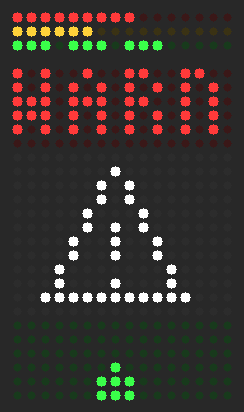
\includegraphics[width=\linewidth]{figures/warn2.png}\\[-2pt]
{\scriptsize\color{grey}}
\end{minipage}\hspace{4pt}%
\begin{minipage}[t]{3.20cm}\centering
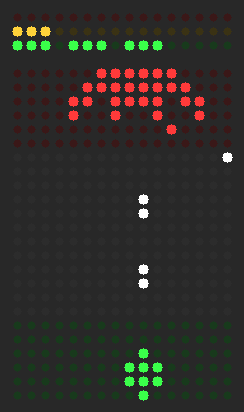
\includegraphics[width=\linewidth]{figures/bossdown.png}\\[-2pt]
{\scriptsize\color{grey}}
\end{minipage}\hspace{4pt}%
\begin{minipage}[t]{3.20cm}\centering
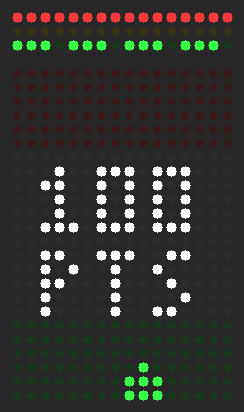
\includegraphics[width=\linewidth]{figures/pts.png}\\[-2pt]
{\scriptsize\color{grey}}
\end{minipage}\hspace{4pt}%
\caption{What game.h draws or uses.}
\end{figure}

{\footnotesize\begin{longtable}{|>{\raggedright\arraybackslash}p{5.82cm}|>{\raggedright\arraybackslash}p{10.68cm}|}
\hline\rowcolor{accent}\textbf{\color{white}Function} & \textbf{\color{white}What it does}\\\hline\endhead
stageTime() & ms of game time since the current stage began.\\\hline
\rowcolor{rowshade}setStage(uint8\_t stage) & Switches the phase to another stage and restarts the stage clock.\\\hline
playStageMusic() & The music that belongs to the current stage (also used after a pause).\\\hline
\rowcolor{rowshade}phaseBegin(uint8\_t phase) & Starts a phase: empties the screen, puts the ship back with full ammo, plays the fanfare and begins the INTRO stage.\\\hline
gameStart(uint8\_t phase) & Starts a new game: game clock at 0, the chosen ship, lives and score 0, then the phase (normally phase 1; the test hooks !2 and !3 start later).\\\hline
\rowcolor{rowshade}destroyEnemy(Enemy\& e, bool byPlayer) & Removes an enemy or rock with a boom; a big rock breaks into two small ones. Destroyed by the player (byPlayer), it also gives points and maybe drops a pickup.\\\hline
hitEnemy(Enemy\& e) & A player bullet hits an enemy: it loses one health point and disappears for a moment, or it is destroyed when it had only one left.\\\hline
\rowcolor{rowshade}pointIn(int8\_t px, int8\_t py, int8\_t x, int8\_t y, uint8\_t w, uint8\_t h) & True when the point (px, py) lies inside the box at (x, y) of size w x h.\\\hline
playerShotHits(Shot\& s) & A player bullet against enemies, the boss and mines.\\\hline
\rowcolor{rowshade}shotsStep() & Moves every bullet and mine one pixel when its time comes (player bullets up, enemy bullets down and maybe sideways) and checks what each of them hits.\\\hline
enemyTouchesShip(const Enemy\& e) & True when a lit pixel of the enemy or rock lies on a lit pixel of the ship, so the empty corners of a hollow rock (or between a drone's wings) don't count as a crash.\\\hline
\rowcolor{rowshade}contactsStep() & Flying into an enemy, a rock or the boss also costs a life.\\\hline
collect(Pickup\& p) & The ship caught a pickup: ammo crate = more ammo (up to the ship's maximum), plus = one extra life (up to 4). Both give 5 points.\\\hline
\rowcolor{rowshade}pickupsStep() & Lets the pickups fall, checks whether the ship catches one, and sends an ammo crate when the player is about to run out.\\\hline
particlesStep() & Moves the explosion pixels and counts down their life (one game step).\\\hline
\rowcolor{rowshade}spawnerStep() & Works through the phase's spawn list: when the wait is over, puts the next enemy, rock or pickup on the screen. Waits while the screen is full, and at SP\_CLEAR until it is empty.\\\hline
bossDown() & The boss has no health left: points, its bullets and helpers vanish, big explosion and screen shake; begins the BOSS\_DOWN stage.\\\hline
\rowcolor{rowshade}phaseClear() & A phase is won: bonus points (100 x phase), one extra life and the 'clear' tune.\\\hline
stageStep() & Runs the current stage for one game step and decides when the next one begins (INTRO -> WAVES -> WARNING -> BOSS -> BOSS\_DOWN -> CLEAR -> next phase). Returns GAME\_OVER or GAME\_WON when the game ends.\\\hline
\rowcolor{rowshade}gameStep() & One game step (20 ms of game time): the ship, enemies, bullets, hits, pickups and explosions each move once, then the stage logic runs.\\\hline
drawGameStatus(uint16\_t frameNo) & Sets the three status bars: red = phase number / wave progress / boss health, yellow = ammo (blinks when low), green = one block of 3 LEDs per life.\\\hline
\rowcolor{rowshade}drawGameTexts() & The messages on top of the game, as still pages (see display.h): INTRO    "ZONE" + the phase number big, then the phase name, then "GO!" WARNING  "WARN" in the red zone and a blinking warning sign CLEAR    "ZONE DONE", the bonus points, "LIFE UP" (if a life was added) demo     every 9 s: "DEMO", then "ANY KEY"\\\hline
drawGame(uint16\_t frameNo) & Draws one picture of the game: pickups, enemies, boss, bullets, ship and explosions (shifted while the screen shakes), then the texts on top and the status bars.\\\hline
\rowcolor{rowshade}gameFrame(uint16\_t frameNo) & One picture of the game: keys, game steps, drawing.\\\hline
gameSkipToBoss() & Test hook !b: removes the enemies and ends the spawn list, so the boss comes next.\\\hline
\rowcolor{rowshade}gamePrintState() & Test hook !s: prints phase, stage, score, lives, ammo, ship position, enemies, boss health and game time over Serial.\\\hline
\end{longtable}}

\subsubsection*{Source code}
\phantomsection\addcontentsline{toc}{subsubsection}{Source code}
\begin{lstlisting}[language=Arduino]
/*
 * game.h -- one game, from PLAY to game over or victory.
 *
 * Each of the three phases runs through these stages:
 *   INTRO      the phase number and name as pages, a short fanfare
 *   WAVES      enemies and rocks arrive from the phase's spawn list (levels.h)
 *   WARNING    "WARN" and a blinking warning sign, a siren, the red bar charges up
 *   BOSS       boss fight with its own music; the red bar shows the boss's health
 *   BOSS_DOWN  the boss blows up, the screen shakes
 *   CLEAR      bonus points and one extra life, then the next phase (after the last
 *              boss the game goes straight to the victory screen)
 * and DEAD when the last life is lost.
 *
 * Status bars: red = phase progress / boss health, yellow = ammo (blinks when low),
 * green = lives (one block of three LEDs per life).
 * The game runs in steps of 20 ms of game time (gameMs); a picture is drawn after each
 * step. Pause simply stops calling it. Test hook !f runs several steps per picture.
 */
#pragma once
#include "world.h"
#include "player.h"
#include "autopilot.h"
#include "enemies.h"
#include "boss.h"
#include "levels.h"

enum GameStage : uint8_t { GS_INTRO, GS_WAVES, GS_WARNING, GS_BOSS, GS_BOSS_DOWN, GS_CLEAR, GS_DEAD };
enum GameResult : uint8_t { GAME_ON, GAME_OVER, GAME_WON };

struct Game {
  uint8_t phase, stage, spawnIndex;
  uint32_t stageStart;                   // gameMs
  uint32_t nextSpawn, nextAmmoHelp, nextBoom;
  uint16_t bonus;
  bool lifeUp;                           // the phase clear gave an extra life
};
Game game;
uint8_t gameSpeed = 1;                   // steps per picture (test hook !f: fast)
bool demoMode = false;                   // the title screen's demo: the autopilot plays

const uint16_t INTRO_MS = 3 * PAGE_MS, WARNING_MS = 3000, BOSS_DOWN_MS = 2500;
const uint16_t CLEAR_MS = 3200, DEAD_MS = 2500;
const uint16_t PICKUP_STEP_MS = 250;
const uint8_t DROP_CHANCE = 12;          // % chance that a destroyed enemy drops ammo

// ms of game time since the current stage began.
uint32_t stageTime() {
  return gameMs - game.stageStart;
}

// Switches the phase to another stage and restarts the stage clock.
void setStage(uint8_t stage) {
  game.stage = stage;
  game.stageStart = gameMs;
}

// The music that belongs to the current stage (also used after a pause).
void playStageMusic() {
  const PhaseInfo& ph = PHASES[game.phase];
  if (game.stage == GS_WAVES) soundPlaySong(ph.song, ph.songTickMs, true);
  else if (game.stage == GS_BOSS) soundPlaySong(SONG_BOSS, SONG_BOSS_TICK_MS, true);
}

// Starts a phase: empties the screen, puts the ship back with full ammo, plays the
// fanfare and begins the INTRO stage.
void phaseBegin(uint8_t phase) {
  game.phase = phase;
  game.spawnIndex = 0;
  game.nextAmmoHelp = 0;
  worldClear();
  playerStart(false);
  setStage(GS_INTRO);
  soundStop();
  soundPlaySong(SONG_STING, 100, false);
  Serial.print(F("[VR] phase "));
  Serial.println(phase + 1);
}

// Starts a new game: game clock at 0, the chosen ship, lives and score 0, then the phase
// (normally phase 1; the test hooks !2 and !3 start later).
void gameStart(uint8_t phase) {
  gameMs = 0;
  playerStart(true);
  phaseBegin(phase);
}

// ================================================================= hits and pickups
// Removes an enemy or rock with a boom; a big rock breaks into two small ones. Destroyed
// by the player (byPlayer), it also gives points and maybe drops a pickup.
void destroyEnemy(Enemy& e, bool byPlayer) {
  const EnemyInfo& info = infoOf(e);
  int8_t x = e.x, y = e.y;
  uint8_t type = e.type;
  e.alive = false;                       // it just vanishes: flying debris only for the
  soundSfx(SFX(SFX_BOOM), 3);            // boss and the player's ship (easier to read)
  if (type == EN_ROCK_B) {               // a big rock breaks into two small ones
    const int8_t w = ENEMY_INFO[EN_ROCK_S].w;          // side by side, also at the edges
    const int8_t ax = constrain(x - 1, 0, SCREEN_W - 2 * w);
    Enemy* a = spawnEnemy(EN_ROCK_S, ax, y);
    Enemy* b = spawnEnemy(EN_ROCK_S, ax + w, y);
    if (a) a->dir = -1;
    if (b) b->dir = 1;
  }
  if (!byPlayer) return;
  addScore(info.score);
  if (type == EN_CRUISER && player.lives < MAX_LIVES) spawnPickup(PK_LIFE, x + 1, y);
  else if (random(100) < DROP_CHANCE && !pickupAlive(PK_AMMO)) spawnPickup(PK_AMMO, x, y);
}

// A player bullet hits an enemy: it loses one health point and disappears for a moment,
// or it is destroyed when it had only one left.
void hitEnemy(Enemy& e) {
  if (e.hp > 1) {
    e.hp--;
    e.flash = 6;
    soundSfx(SFX(SFX_HIT), 2);
  } else {
    destroyEnemy(e, true);
  }
}

// True when the point (px, py) lies inside the box at (x, y) of size w x h.
bool pointIn(int8_t px, int8_t py, int8_t x, int8_t y, uint8_t w, uint8_t h) {
  return px >= x && px < x + w && py >= y && py < y + h;
}

// A player bullet against enemies, the boss and mines.
void playerShotHits(Shot& s) {
  for (uint8_t i = 0; i < MAX_ENEMIES; i++) {
    Enemy& e = enemies[i];
    if (e.alive && pointIn(s.x, s.y, e.x, e.y, infoOf(e).w, infoOf(e).h)) {
      s.alive = false;
      hitEnemy(e);
      return;
    }
  }
  if (game.stage == GS_BOSS && boss.alive && boss.hp > 0 &&
      pointIn(s.x, s.y, boss.x, boss.y, boss.w, boss.h)) {
    s.alive = false;
    boss.hp--;                           // (no flash: the red bar and the sound show it)
    soundSfx(SFX(SFX_HIT), 2);
    return;
  }
  for (uint8_t i = 0; i < MAX_SHOTS; i++) {   // mines can be shot too
    Shot& m = shots[i];
    if (m.alive && m.kind == SHOT_MINE && m.x == s.x && (m.y == s.y || m.y == s.y + 1)) {
      m.alive = s.alive = false;
      addScore(2);
      soundSfx(SFX(SFX_HIT), 2);
      return;
    }
  }
}

// Moves every bullet and mine one pixel when its time comes (player bullets up, enemy
// bullets down and maybe sideways) and checks what each of them hits.
void shotsStep() {
  for (uint8_t i = 0; i < MAX_SHOTS; i++) {
    Shot& s = shots[i];
    if (!s.alive) continue;
    if (gameMs >= s.next) {
      s.next += s.stepMs;
      s.y += (s.kind == SHOT_PLAYER) ? -1 : 1;
      if (s.dx && ++s.sideCount >= s.sideEvery) {
        s.x += s.dx;
        s.sideCount = 0;
      }
      if (s.y < 0 || s.y >= SCREEN_H || s.x < 0 || s.x >= SCREEN_W) {
        s.alive = false;
        continue;
      }
    }
    if (s.kind == SHOT_PLAYER) playerShotHits(s);
    else if (shipPixel(s.x, s.y) && !playerShielded() && player.lives) {
      s.alive = false;
      playerHit(s.kind == SHOT_MINE ? F("mine") : F("shot"));
    }
  }
}

// True when a lit pixel of the enemy or rock lies on a lit pixel of the ship, so the empty
// corners of a hollow rock (or between a drone's wings) don't count as a crash.
bool enemyTouchesShip(const Enemy& e) {
  const EnemyInfo& info = infoOf(e);
  if (!boxesTouch(e.x, e.y, info.w, info.h, player.x, player.y, 3, 3)) return false;
  for (uint8_t r = 0; r < info.h; r++) {
    uint16_t bits = pgm_read_word(info.sprite + r);
    for (uint8_t c = 0; c < info.w; c++)
      if ((bits & (0x8000u >> c)) && shipPixel(e.x + c, e.y + r)) return true;
  }
  return false;
}

// Flying into an enemy, a rock or the boss also costs a life.
void contactsStep() {
  if (playerShielded() || player.lives == 0) return;
  for (uint8_t i = 0; i < MAX_ENEMIES; i++) {
    Enemy& e = enemies[i];
    if (e.alive && enemyTouchesShip(e)) {
      bool rock = e.type >= EN_ROCK_S;
      destroyEnemy(e, false);
      playerHit(rock ? F("rock") : F("enemy"));
      return;
    }
  }
  if (game.stage == GS_BOSS && boss.alive &&
      boxesTouch(boss.x, boss.y, boss.w, boss.h, player.x, player.y, 3, 3))
    playerHit(F("boss"));
}

// The ship caught a pickup: ammo crate = more ammo (up to the ship's maximum), plus =
// one extra life (up to 4). Both give 5 points.
void collect(Pickup& p) {
  p.alive = false;
  addScore(5);
  if (p.type == PK_AMMO) {
    uint8_t room = playerShip().ammoMax - player.ammo, pack = DIFF_PACK_AMMO[settings.difficulty];
    player.ammo += pack < room ? pack : room;
    if (player.ammo > LOW_AMMO) player.lowAmmoWarned = false;
    soundSfx(SFX(SFX_PICKUP), 4);
    Serial.println(F("[VR] pickup ammo"));
  } else {
    if (player.lives < MAX_LIVES) player.lives++;
    soundSfx(SFX(SFX_LIFE), 4);
    Serial.println(F("[VR] pickup life"));
  }
}

// Lets the pickups fall, checks whether the ship catches one, and sends an ammo crate
// when the player is about to run out.
void pickupsStep() {
  for (uint8_t i = 0; i < MAX_PICKUPS; i++) {
    Pickup& p = pickups[i];
    if (!p.alive) continue;
    if (gameMs >= p.next) {
      p.next += PICKUP_STEP_MS;
      if (++p.y >= SCREEN_H) p.alive = false;
    }
    if (p.alive && player.lives && boxesTouch(p.x, p.y, 3, 3, player.x, player.y, 3, 3)) collect(p);
  }
  // Running out of ammo: a crate is sent, so the game can always go on.
  bool fighting = game.stage == GS_WAVES || game.stage == GS_BOSS;
  if (fighting && player.ammo <= LOW_AMMO && !pickupAlive(PK_AMMO) && gameMs >= game.nextAmmoHelp) {
    spawnPickup(PK_AMMO, random(SCREEN_W - 2), -3);
    game.nextAmmoHelp = gameMs + 5000;
  }
}

// Moves the explosion pixels and counts down their life (one game step).
void particlesStep() {
  for (uint8_t i = 0; i < MAX_PARTICLES; i++) {
    Particle& p = particles[i];
    if (!p.life) continue;
    p.x16 += p.vx;
    p.y16 += p.vy;
    p.life--;
  }
}

// ================================================================= phase flow
// Works through the phase's spawn list: when the wait is over, puts the next enemy,
// rock or pickup on the screen. Waits while the screen is full, and at SP_CLEAR until
// it is empty.
void spawnerStep() {
  const PhaseInfo& ph = PHASES[game.phase];
  while (game.spawnIndex < ph.count && gameMs >= game.nextSpawn) {
    Spawn s = spawnAt(game.phase, game.spawnIndex);
    if (s.what == SP_CLEAR && enemiesAlive()) return;       // wait for an empty screen
    if (s.what < SP_AMMO && enemiesAlive() >= ph.maxEnemies) return;   // screen is full
    if (s.what == SP_AMMO) spawnPickup(PK_AMMO, s.x, -3);
    else if (s.what == SP_LIFE) spawnPickup(PK_LIFE, s.x, -3);
    else if (s.what < SP_AMMO) spawnFromTable(s.what, s.x);
    if (++game.spawnIndex < ph.count)
      game.nextSpawn = gameMs + spawnAt(game.phase, game.spawnIndex).wait * 100UL;
  }
}

// The boss has no health left: points, its bullets and helpers vanish, big explosion and
// screen shake; begins the BOSS_DOWN stage.
void bossDown() {
  addScore(BOSS_SCORE[boss.kind]);
  for (uint8_t i = 0; i < MAX_SHOTS; i++)           // its bullets vanish ...
    if (shots[i].kind != SHOT_PLAYER) shots[i].alive = false;
  for (uint8_t i = 0; i < MAX_ENEMIES; i++)         // ... and so do its helpers
    enemies[i].alive = false;
  setStage(GS_BOSS_DOWN);
  game.nextBoom = gameMs;
  soundStop();
  soundSfx(SFX(SFX_BIG_BOOM), 5);
  shake(40);
  Serial.println(F("[VR] boss down"));
}

// A phase is won: bonus points (100 x phase), one extra life and the 'clear' tune.
void phaseClear() {
  game.bonus = PHASE_BONUS * (game.phase + 1);
  addScore(game.bonus);
  game.lifeUp = player.lives < MAX_LIVES;
  if (game.lifeUp) player.lives++;
  setStage(GS_CLEAR);
  soundPlaySong(SONG_CLEAR, 90, false);
  Serial.println(F("[VR] phase clear"));
}

// Runs the current stage for one game step and decides when the next one begins
// (INTRO -> WAVES -> WARNING -> BOSS -> BOSS_DOWN -> CLEAR -> next phase).
// Returns GAME_OVER or GAME_WON when the game ends.
GameResult stageStep() {
  const PhaseInfo& ph = PHASES[game.phase];
  switch (game.stage) {
    case GS_INTRO:
      if (stageTime() >= INTRO_MS) {
        setStage(GS_WAVES);
        playStageMusic();
        game.nextSpawn = gameMs + spawnAt(game.phase, 0).wait * 100UL;
      }
      break;
    case GS_WAVES:
      spawnerStep();
      if (game.spawnIndex >= ph.count && !enemiesAlive()) {
        setStage(GS_WARNING);
        soundStop();
        soundSfx(SFX(SFX_SIREN), 5);
        Serial.println(F("[VR] warning"));
      }
      break;
    case GS_WARNING:
      if (stageTime() >= WARNING_MS) {
        bossStart(ph.boss);
        setStage(GS_BOSS);
        playStageMusic();
        Serial.println(F("[VR] boss"));
      }
      break;
    case GS_BOSS:
      updateBoss();
      if (boss.hp <= 0) bossDown();
      break;
    case GS_BOSS_DOWN:
      boss.flash = 2;                                 // keeps blinking while it burns
      if (stageTime() < 1500 && gameMs >= game.nextBoom) {
        explode(boss.x + random(boss.w), boss.y + random(boss.h), 6, 12);
        game.nextBoom = gameMs + 120;
      }
      if (boss.alive && stageTime() >= 1500) {        // final blast
        boss.alive = false;
        explode(boss.x + boss.w / 2, boss.y + boss.h / 2, 30, 16);
        shake(20);
        soundSfx(SFX(SFX_BIG_BOOM), 5);
      }
      if (stageTime() >= BOSS_DOWN_MS) {
        if (game.phase == 2) {                        // last boss: bonus, then straight to
          addScore(PHASE_BONUS * 3);                  // the victory screen (no ZONE DONE,
          return GAME_WON;                            // no extra life)
        }
        phaseClear();
      }
      break;
    case GS_CLEAR:
      if (stageTime() >= CLEAR_MS) {
        if (game.phase == 2) return GAME_WON;
        phaseBegin(game.phase + 1);
      }
      break;
    case GS_DEAD:
      if (stageTime() >= DEAD_MS) return GAME_OVER;
      break;
  }
  return GAME_ON;
}

// One game step (20 ms of game time): the ship, enemies, bullets, hits, pickups and
// explosions each move once, then the stage logic runs.
GameResult gameStep() {
  gameMs += FRAME_MS;
  if (autopilot) autopilotStep();
  playerStep();
  updateEnemies();
  shotsStep();
  contactsStep();
  pickupsStep();
  particlesStep();
  if (player.lives == 0 && game.stage != GS_DEAD) {   // the last life is gone
    setStage(GS_DEAD);
    explode(player.x + 1, player.y + 1, 25, 16);
    shake(30);
    soundStop();
    soundSfx(SFX(SFX_BIG_BOOM), 6);
    Serial.print(F("[VR] game over score="));
    Serial.println(player.score);
  }
  return stageStep();
}

// ================================================================= drawing
// Sets the three status bars: red = phase number / wave progress / boss health,
// yellow = ammo (blinks when low), green = one block of 3 LEDs per life.
void drawGameStatus(uint16_t frameNo) {
  uint8_t red = 0;                       // red: phase progress / boss charging / boss health
  if (game.stage == GS_WAVES) red = (uint16_t)game.spawnIndex * 16 / PHASES[game.phase].count;
  if (game.stage == GS_WARNING && (frameNo & 8)) red = stageTime() * 16 / WARNING_MS;
  if (game.stage == GS_BOSS && boss.hp > 0) red = (boss.hp * 16 + boss.maxHp - 1) / boss.maxHp;
  if (game.stage == GS_CLEAR && (frameNo & 8)) red = 16;
  if (game.stage == GS_INTRO) {          // phase number: one block per phase
    uint16_t blocks = 0;
    for (uint8_t i = 0; i <= game.phase; i++) blocks |= 0x7u << (i * 4);
    setStatusBits(0, blocks);
  } else {
    setStatusBar(0, red);
  }
  uint8_t ammoMax = playerShip().ammoMax;   // yellow: ammo, blinks when low
  uint8_t yellow = ((uint16_t)player.ammo * 16 + ammoMax - 1) / ammoMax;
  if (player.ammo <= LOW_AMMO && (frameNo & 8)) yellow = 0;
  setStatusBar(1, yellow);
  uint16_t lives = 0;                    // green: one block of three LEDs per life
  for (uint8_t i = 0; i < player.lives; i++) lives |= 0x7u << (i * 4);
  setStatusBits(2, lives);
}

// The messages on top of the game, as still pages (see display.h):
//   INTRO    "ZONE" + the phase number big, then the phase name, then "GO!"
//   WARNING  "WARN" in the red zone and a blinking warning sign
//   CLEAR    "ZONE DONE", the bonus points, "LIFE UP" (if a life was added)
//   demo     every 9 s: "DEMO", then "ANY KEY"
void drawGameTexts() {
  const PhaseInfo& ph = PHASES[game.phase];
  uint32_t t = stageTime();
  if (game.stage == GS_INTRO) {
    uint8_t page = pageAt(t, 3);
    if (page == 0) {
      clearRows(0, 18);
      drawTextCentered(0, PSTR("ZONE"), false);
      drawChar(5, 7, '1' + game.phase, false, 2);      // 6 x 10 pixels
    } else if (page == 1) {
      drawPage(ph.name1, ph.name2);
    } else {
      drawPage(PSTR("GO!"), NULL);
    }
  } else if (game.stage == GS_WARNING) {
    clearRows(0, 5);
    drawTextCentered(0, PSTR("WARN"), false);
    if ((t / 300) % 2) drawBitmap(2, 7, WARNING_SIGN, 11, 10, true);
  } else if (game.stage == GS_CLEAR) {
    uint8_t page = pageAt(t, 3);
    if (page == 1) {
      clearRows(6, 12);
      drawNumberCentered(7, game.bonus, false);
      drawTextCentered(13, PSTR("PTS"), false);
    } else if (page == 2 && game.lifeUp) {
      drawPage(PSTR("LIFE"), PSTR("UP"));
    } else {
      drawPage(PSTR("ZONE"), PSTR("DONE"));
    }
  } else if (demoMode && gameMs % 9000 < 2 * PAGE_MS) {
    if (pageAt(gameMs % 9000, 2) == 0) drawPage(PSTR("DEMO"), NULL);
    else drawPage(PSTR("ANY"), PSTR("KEY"));
  }
}

// Draws one picture of the game: pickups, enemies, boss, bullets, ship and explosions
// (shifted while the screen shakes), then the texts on top and the status bars.
void drawGame(uint16_t frameNo) {
  if (shakeFrames) {                     // screen shake: everything moves one pixel
    shakeFrames--;
    shakeX = random(-1, 2);
    shakeY = random(-1, 2);
  }
  clearScreen();
  for (uint8_t i = 0; i < MAX_PICKUPS; i++) {
    const Pickup& p = pickups[i];
    if (p.alive && (p.type == PK_AMMO || (frameNo & 8)))   // the life blinks
      drawBitmap(p.x, p.y, p.type == PK_AMMO ? PICKUP_AMMO : PICKUP_LIFE, 3, 3, true);
  }
  drawEnemies();
  drawBoss(frameNo);
  for (uint8_t i = 0; i < MAX_SHOTS; i++) {
    const Shot& s = shots[i];
    if (!s.alive) continue;
    if (s.kind == SHOT_PLAYER) {         // player bullet: a short streak
      setPixel(s.x, s.y, true);
      setPixel(s.x, s.y + 1, true);
    } else {                             // enemy bullet or mine: one steady pixel
      setPixel(s.x, s.y, true);
    }
  }
  drawPlayer(frameNo);
  for (uint8_t i = 0; i < MAX_PARTICLES; i++)
    if (particles[i].life) setPixel(particles[i].x16 >> 4, particles[i].y16 >> 4, true);
  shakeX = shakeY = 0;

  drawGameTexts();
  drawGameStatus(frameNo);
}

// One picture of the game: keys, game steps, drawing.
GameResult gameFrame(uint16_t frameNo) {
  playerKeys();
  GameResult result = GAME_ON;
  for (uint8_t i = 0; i < gameSpeed && result == GAME_ON; i++) result = gameStep();
  drawGame(frameNo);
  return result;
}

// ================================================================= test hooks
// Test hook !b: removes the enemies and ends the spawn list, so the boss comes next.
void gameSkipToBoss() {
  for (uint8_t i = 0; i < MAX_ENEMIES; i++) enemies[i].alive = false;
  if (game.stage > GS_WAVES) return;
  game.spawnIndex = PHASES[game.phase].count;
  if (game.stage == GS_INTRO) setStage(GS_WAVES);
}

// Test hook !s: prints phase, stage, score, lives, ammo, ship position, enemies, boss
// health and game time over Serial.
void gamePrintState() {
  Serial.print(F("[VR] state phase="));
  Serial.print(game.phase + 1);
  Serial.print(F(" stage="));
  Serial.print(game.stage);
  Serial.print(F(" score="));
  Serial.print(player.score);
  Serial.print(F(" lives="));
  Serial.print(player.lives);
  Serial.print(F(" ammo="));
  Serial.print(player.ammo);
  Serial.print(F(" x="));
  Serial.print(player.x);
  Serial.print(F(" y="));
  Serial.print(player.y);
  Serial.print(F(" enemies="));
  Serial.print(enemiesAlive());
  Serial.print(F(" boss="));
  Serial.print(boss.alive ? boss.hp : 0);
  Serial.print(F(" t="));
  Serial.println(gameMs);
}
\end{lstlisting}

\clearpage
\subsection*{4.20 autopilot.h – Autopilot}
\phantomsection\addcontentsline{toc}{subsection}{4.20 autopilot.h – Autopilot}
A bot that plays like a careful player. It is used by the title screen's demo and by the automatic tests: for every column it works out how soon something would hit the ship there, flies to the safest column near its target and fires when lined up.

\begin{figure}[H]\centering
\begin{minipage}[t]{3.60cm}\centering
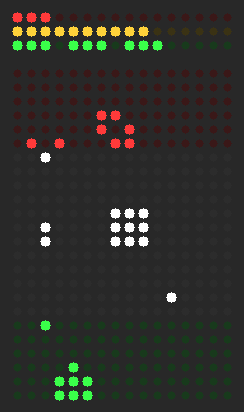
\includegraphics[width=\linewidth]{figures/phase1_3.png}\\[-2pt]
{\scriptsize\color{grey}}
\end{minipage}\hspace{4pt}%
\caption{What autopilot.h draws or uses.}
\end{figure}

\par\noindent\begin{minipage}{\linewidth}\centering\footnotesize
\begin{tabular}{|>{\raggedright\arraybackslash}p{5.82cm}|>{\raggedright\arraybackslash}p{10.68cm}|}
\hline\rowcolor{accent}\textbf{\color{white}Function} & \textbf{\color{white}What it does}\\\hline
minMs(int32\_t a, int32\_t b) & Returns the smaller of two times (ms).\\\hline
\rowcolor{rowshade}impactMs(int8\_t c) & ms until something touches the ship if it stands with its left edge in column c.\\\hline
autopilotTarget() & Chooses what the autopilot aims at: an ammo crate when ammo is low, otherwise the boss, otherwise the lowest enemy above the ship. Returns that column, or -1 if there is none.\\\hline
\rowcolor{rowshade}autopilotStep() & The autopilot's turn (every game step while !x or the demo is on): when the ship may move again it picks the best reachable column and moves one pixel toward it, or fires when it is lined up under its target.\\\hline
\end{tabular}
\end{minipage}\par\medskip

\subsubsection*{Source code}
\phantomsection\addcontentsline{toc}{subsubsection}{Source code}
\begin{lstlisting}[language=Arduino]
/*
 * autopilot.h -- test hook (!x): the ship flies itself, like a careful player.
 *
 * Used by the automatic tests to play whole games and to check that every phase can be
 * won without the shield. It follows the same rule as a player (it either moves or
 * fires, never both) and stays on the bottom row.
 *
 * How it decides, each time the ship could move one pixel:
 *   1. For every column it works out how many ms are left before a bullet, an enemy or
 *      a rock would touch the ship standing there ("time to impact").
 *   2. A column is reachable if the ship can fly there, one pixel per moveMs, without
 *      passing a column where something hits it on the way.
 *   3. Of the reachable columns that stay safe for a while, it takes the one nearest its
 *      target (an ammo crate when ammo is low, else the boss or the lowest enemy); if
 *      none is safe, the one where the danger arrives last.
 *   4. Lined up under the target in a safe column, it fires.
 */
#pragma once
#include "world.h"
#include "player.h"

const int32_t AUTO_NO_DANGER = 100000;   // "nothing will hit this column"
const int32_t AUTO_SAFE_MS = 450;        // a column must stay clear this long to stop in
#ifndef AUTOPILOT_REACT_MS
#define AUTOPILOT_REACT_MS 0             // PC tests: > 0 = rethinks only this often (slower)
#endif

// Returns the smaller of two times (ms).
int32_t minMs(int32_t a, int32_t b) {
  return a < b ? a : b;
}

// ms until something touches the ship if it stands with its left edge in column c.
int32_t impactMs(int8_t c) {
  int8_t top = player.y, bottom = player.y + 2;
  int32_t first = AUTO_NO_DANGER;
  for (uint8_t i = 0; i < MAX_SHOTS; i++) {               // enemy bullets and mines
    const Shot& s = shots[i];
    if (!s.alive || s.kind == SHOT_PLAYER || s.y > bottom) continue;
    for (int8_t r = top; r <= bottom; r++) {
      int8_t down = r - s.y;                               // rows still to fall
      if (down < 0) continue;
      int8_t col = s.x + (s.dx ? s.dx * ((down + s.sideCount) / s.sideEvery) : 0);
      if (col < c || col > c + 2) continue;
      int32_t t = down ? (int32_t)(s.next - gameMs) + (int32_t)(down - 1) * s.stepMs : 0;
      first = minMs(first, t);
    }
  }
  for (uint8_t i = 0; i < MAX_ENEMIES; i++) {             // enemies and rocks coming down
    const Enemy& e = enemies[i];
    bool staysUp = e.type == EN_MINER || (e.type == EN_CRUISER && e.y >= 3);   // no longer sink
    if (!e.alive || staysUp || e.y > bottom) continue;
    const EnemyInfo& info = infoOf(e);
    int8_t margin = e.type == EN_WEAVER ? 2 : (e.type >= EN_ROCK_S ? 1 : 0);   // side moves
    if (e.x - margin > c + 2 || e.x + info.w - 1 + margin < c) continue;
    int8_t down = top - (e.y + info.h - 1);
    int32_t wait = (int32_t)(e.nextMove - gameMs);        // until its next step down
    int32_t t = down <= 0 ? 0 : (wait > 0 ? wait : 0) + (int32_t)(down - 1) * info.stepMs;
    first = minMs(first, t);
  }
  if (boss.alive && boss.y + boss.h > top && boss.x <= c + 2 && boss.x + boss.w > c)
    first = 0;                                             // the boss itself
  return first;
}

// Chooses what the autopilot aims at: an ammo crate when ammo is low, otherwise the boss,
// otherwise the lowest enemy above the ship. Returns that column, or -1 if there is none.
int8_t autopilotTarget() {
  if (player.ammo <= LOW_AMMO)
    for (uint8_t i = 0; i < MAX_PICKUPS; i++)
      if (pickups[i].alive && pickups[i].type == PK_AMMO) return pickups[i].x;
  if (boss.alive) return boss.x + boss.w / 2 - 1;
  int8_t target = -1, lowest = -100;
  for (uint8_t i = 0; i < MAX_ENEMIES; i++) {
    const Enemy& e = enemies[i];
    if (e.alive && e.y > lowest && e.y < player.y - 6 && e.x >= 0 && e.x < SCREEN_W) {
      lowest = e.y;
      target = e.x + infoOf(e).w / 2 - 1;
    }
  }
  return target < 0 ? -1 : constrain(target, 0, SCREEN_W - 3);
}

// The autopilot's turn (every game step while !x or the demo is on): when the ship may
// move again it picks the best reachable column and moves one pixel toward it, or fires
// when it is lined up under its target.
void autopilotStep() {
  if (player.lives == 0 || gameMs < player.nextMove) return;
  if (player.y < PLAYER_MAX_Y) {                           // go to the bottom row first
    movePlayer(KEY_DOWN);
    player.firing = false;
    player.nextMove = gameMs + playerShip().moveMs;
    return;
  }
  int32_t moveMs = playerShip().moveMs;
  static int8_t plan = -1;                                 // column chosen last time
  static uint32_t nextThink = 0;
  if (AUTOPILOT_REACT_MS && gameMs < nextThink && plan >= 0) {   // still reacting
    if (plan != player.x) {
      movePlayer(plan > player.x ? KEY_RIGHT : KEY_LEFT);
      player.firing = false;
    }
    player.nextMove = gameMs + moveMs;
    return;
  }
  int32_t impact[SCREEN_W - 2];
  for (int8_t c = 0; c <= SCREEN_W - 3; c++) impact[c] = impactMs(c);

  int8_t target = autopilotTarget();
  int8_t best = player.x;
  int32_t bestSpare = -AUTO_NO_DANGER;                     // fallback: latest danger
  int16_t bestDistance = 1000;                             // among safe columns
  bool bestSafe = false;
  for (int8_t dir = -1; dir <= 1; dir += 2) {
    for (int8_t c = player.x, steps = 0; c >= 0 && c <= SCREEN_W - 3; c += dir, steps++) {
      if (dir > 0 && steps == 0) continue;                 // the own column is checked once
      int32_t arrive = steps * moveMs;
      if (steps && impact[c] <= arrive + moveMs) break;    // would be hit on the way
      int32_t spare = impact[c] - arrive;
      bool safe = spare > AUTO_SAFE_MS;
      int16_t distance = (target >= 0 ? abs(c - target) * 4 : 0) + steps;
      if ((safe && (!bestSafe || distance < bestDistance)) || (!bestSafe && !safe && spare > bestSpare)) {
        best = c;
        bestSafe = safe;
        bestSpare = spare;
        bestDistance = distance;
      }
    }
  }
  plan = best;
  nextThink = gameMs + AUTOPILOT_REACT_MS;
  bool linedUp = target >= 0 && abs(target - player.x) <= 1 && player.ammo > 0;
  if (best != player.x) {
    movePlayer(best > player.x ? KEY_RIGHT : KEY_LEFT);   // moving: no fire
    player.firing = false;
  } else if (linedUp && impact[player.x] > AUTO_SAFE_MS) {
    if (!player.firing) player.burst = 0;                  // like pressing R
    player.firing = true;
  } else {
    player.firing = false;
  }
  player.nextMove = gameMs + moveMs;
}
\end{lstlisting}

\clearpage
\subsection*{4.21 screens.h – The other screens}
\phantomsection\addcontentsline{toc}{subsection}{4.21 screens.h – The other screens}
The hangar, the options (with the LED test), the best score, pause, game over and victory. Each screen function handles its keys, draws one picture and returns the next screen.

\begin{figure}[H]\centering
\begin{minipage}[t]{3.00cm}\centering
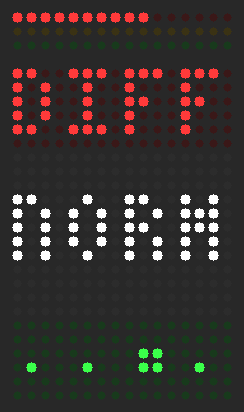
\includegraphics[width=\linewidth]{figures/opt_diff.png}\\[-2pt]
{\scriptsize\color{grey}}
\end{minipage}\hspace{4pt}%
\begin{minipage}[t]{3.00cm}\centering
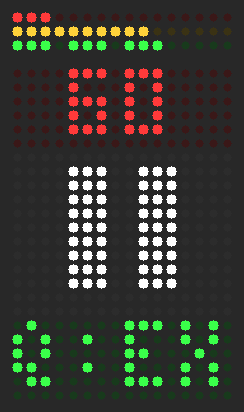
\includegraphics[width=\linewidth]{figures/pause_sign.png}\\[-2pt]
{\scriptsize\color{grey}}
\end{minipage}\hspace{4pt}%
\begin{minipage}[t]{3.00cm}\centering
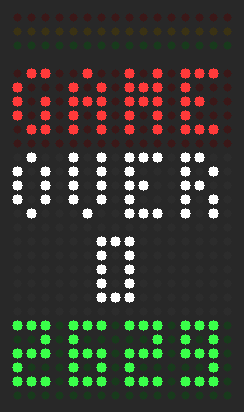
\includegraphics[width=\linewidth]{figures/over1.png}\\[-2pt]
{\scriptsize\color{grey}}
\end{minipage}\hspace{4pt}%
\begin{minipage}[t]{3.00cm}\centering
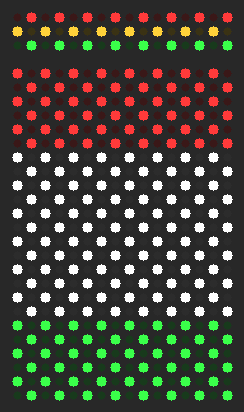
\includegraphics[width=\linewidth]{figures/led4.png}\\[-2pt]
{\scriptsize\color{grey}}
\end{minipage}\hspace{4pt}%
\caption{What screens.h draws or uses.}
\end{figure}

{\footnotesize\begin{longtable}{|>{\raggedright\arraybackslash}p{5.82cm}|>{\raggedright\arraybackslash}p{10.68cm}|}
\hline\rowcolor{accent}\textbf{\color{white}Function} & \textbf{\color{white}What it does}\\\hline\endhead
applyBrightness() & Sets the LED brightness from the saved setting (100 / 50 / 20 \%).\\\hline
\rowcolor{rowshade}drawSideArrows(int8\_t y, uint16\_t frameNo) & Small arrows at the left and right edge: "A/D changes this".\\\hline
drawPageDots(uint8\_t count, uint8\_t current) & One dot per page at the bottom; the current page is a bigger block.\\\hline
\rowcolor{rowshade}clearStatusBars() & Switches off all three status bars.\\\hline
hangarBegin() & Opens the hangar on the ship that is in use now.\\\hline
\rowcolor{rowshade}hangarFrame(uint32\_t now, uint16\_t frameNo) & One picture of the hangar: A/D (or W/S) shows another ship, R takes it (saved), Q goes back. Draws name, big ship, arrows and page dots; the stats go on the status bars.\\\hline
optionsFrame(uint16\_t frameNo) & One picture of the options: W/S picks LITE, SND, DIFF or TEST; A/D or R changes it (saved in the EEPROM); R on TEST starts the LED test; Q goes back.\\\hline
\rowcolor{rowshade}bestFrame(uint16\_t frameNo) & One picture of the BEST page: the high score, then (bottom line, changing every 1.2 s) how far it got - "ZONE" and 1-3, or "WIN" - and the difficulty it was made on.\\\hline
pauseDraw(uint32\_t t, uint16\_t frameNo) & Draws the pause screen: the score, a big pause sign, and the keys as a page that changes every 1.2 s ("P:GO" = P continues, "Q:EX" = Q exits), with the game's bars.\\\hline
\rowcolor{rowshade}recordScore(uint8\_t phaseReached) & Saves the score as the new best (with the phase reached, 4 = won, and the difficulty) if it beats the old one. The score counts first; the same score on a harder difficulty also takes the record.\\\hline
gameOverFrame(uint32\_t t, uint16\_t frameNo) & One picture of GAME OVER: the score (blinking if it is a record) and the best score; after 1 s, R or Q goes to the menu.\\\hline
\rowcolor{rowshade}victoryFrame(uint32\_t t) & One picture of the victory screen: fireworks, pages "YOU WIN!", "VOID SAFE" and the score, and racing status bars; after 2 s, R or Q goes to the menu.\\\hline
ledTestSetRow(uint8\_t fromTop, uint16\_t bits) & Sets one matrix row, counted from the top as built (status bars first, then the game screen).\\\hline
\rowcolor{rowshade}ledTestFrame(uint32\_t t) & One picture of the LED test: all on, then each row, each column and a checkerboard, with a rising beep per step. Any key (or the end) goes back to the options.\\\hline
\end{longtable}}

\subsubsection*{Source code}
\phantomsection\addcontentsline{toc}{subsubsection}{Source code}
\begin{lstlisting}[language=Arduino]
/*
 * screens.h -- the screens around the game:
 *   HANGAR    choose a ship (A/D), R = take it, Q = back.
 *             Status bars: red = speed, yellow = ammo, green = fire power.
 *   OPTIONS   W/S = item, A/D or R = change: LITE (brightness), SND (sound),
 *             DIFF (difficulty), TEST (LED test). Saved in the EEPROM.
 *   BEST      the high score and how far it got.
 *   PAUSE     P or R = continue, Q = quit to the menu.
 *   GAME OVER / VICTORY   the score; R or Q = menu.
 *   LED TEST  every LED on, then row, column and checker patterns (hardware check).
 * Each xxxFrame() handles the keys, draws one picture and returns the screen to show
 * next (its own screen to stay).
 */
#pragma once
#include "display.h"
#include "input.h"
#include "sound.h"
#include "storage.h"
#include "world.h"
#include "game.h"

// Sets the LED brightness from the saved setting (100 / 50 / 20 %).
void applyBrightness() {
  displaySetBrightness(BRIGHTNESS_LEVELS[settings.brightness]);
}

// Small arrows at the left and right edge: "A/D changes this".
void drawSideArrows(int8_t y, uint16_t frameNo) {
  if (frameNo & 16) return;
  setPixel(1, y, true);
  setPixel(0, y + 1, true);
  setPixel(1, y + 2, true);
  setPixel(14, y, true);
  setPixel(15, y + 1, true);
  setPixel(14, y + 2, true);
}

// One dot per page at the bottom; the current page is a bigger block.
void drawPageDots(uint8_t count, uint8_t current) {
  int8_t x = (SCREEN_W - (count * 4 - 2)) / 2;
  for (uint8_t i = 0; i < count; i++, x += 4) {
    if (i == current) fillRect(x, 20, 2, 2, true);
    else setPixel(x, 21, true);
  }
}

// Switches off all three status bars.
void clearStatusBars() {
  for (uint8_t bar = 0; bar < STATUS_ROWS; bar++) setStatusBits(bar, 0);
}

// ================================================================= hangar
uint8_t hangarShip = 0;
uint32_t hangarSwitched = 0;             // millis() when the ship on show changed

// Opens the hangar on the ship that is in use now.
void hangarBegin() {
  hangarShip = settings.ship;
  hangarSwitched = millis();
}

// One picture of the hangar: A/D (or W/S) shows another ship, R takes it (saved), Q goes
// back. Draws name, big ship, arrows and page dots; the stats go on the status bars.
Screen hangarFrame(uint32_t now, uint16_t frameNo) {
  int8_t step = (keyPressed(KEY_RIGHT) || keyPressed(KEY_DOWN)) -
                (keyPressed(KEY_LEFT) || keyPressed(KEY_UP));
  if (step) {
    hangarShip = (hangarShip + 3 + step) % 3;
    hangarSwitched = now;
    soundBeep(1400, 25);
  }
  if (keyPressed(KEY_FIRE)) {
    settings.ship = hangarShip;
    settingsSave();
    soundSfx(SFX(SFX_PICKUP), 4);
    Serial.print(F("[VR] ship "));
    Serial.println((const __FlashStringHelper*)SHIPS[hangarShip].name);
    return SCR_MENU;
  }
  if (keyPressed(KEY_BACK)) return SCR_MENU;

  const ShipInfo& ship = SHIPS[hangarShip];
  clearScreen();
  drawTextCentered(0, ship.name, false);
  drawBitmapScaled(3, 6, ship.sprite, 3, 3, 3);   // the ship, 3 times bigger
  if (frameNo & 1) fillRect(6, 15, 3, 2, true);   // engine flame
  drawSideArrows(9, frameNo);
  drawPageDots(3, hangarShip);
  if (hangarShip == settings.ship) setPixel(SCREEN_W - 1, 23, true);   // the ship in use
  // stats on the status bars, growing in after each switch: 5 LEDs per level
  uint32_t grow = now - hangarSwitched;
  uint8_t levels[3] = {ship.speedLevel, ship.ammoLevel, ship.fireLevel};
  for (uint8_t bar = 0; bar < STATUS_ROWS; bar++) {
    uint8_t full = levels[bar] * 5;
    setStatusBar(bar, grow >= 300 ? full : full * grow / 300);
  }
  return SCR_HANGAR;
}

// ================================================================= options
enum OptionItem : uint8_t { OPT_LITE, OPT_SOUND, OPT_DIFF, OPT_TEST, OPTION_COUNT };
const char OPT_NAME_LITE[] PROGMEM = "LITE";
const char OPT_NAME_SND[] PROGMEM = "SND";
const char OPT_NAME_DIFF[] PROGMEM = "DIFF";
const char OPT_NAME_TEST[] PROGMEM = "TEST";
const char* const OPTION_NAMES[OPTION_COUNT] = {OPT_NAME_LITE, OPT_NAME_SND, OPT_NAME_DIFF, OPT_NAME_TEST};
const char DIFF_EASY_NAME[] PROGMEM = "EASY";
const char DIFF_NORMAL_NAME[] PROGMEM = "NORM";
const char DIFF_HARD_NAME[] PROGMEM = "HARD";
const char* const DIFF_NAMES[3] = {DIFF_EASY_NAME, DIFF_NORMAL_NAME, DIFF_HARD_NAME};
uint8_t optionItem = 0;

// One picture of the options: W/S picks LITE, SND, DIFF or TEST; A/D or R changes it
// (saved in the EEPROM); R on TEST starts the LED test; Q goes back.
Screen optionsFrame(uint16_t frameNo) {
  if (keyPressed(KEY_UP) || keyPressed(KEY_DOWN)) {
    optionItem = (optionItem + (keyPressed(KEY_UP) ? OPTION_COUNT - 1 : 1)) % OPTION_COUNT;
    soundBeep(1400, 25);
  }
  int8_t change = keyPressed(KEY_RIGHT) - keyPressed(KEY_LEFT);
  if (keyPressed(KEY_FIRE)) {
    if (optionItem == OPT_TEST) return SCR_LEDTEST;
    change = 1;
  }
  if (change && optionItem != OPT_TEST) {
    if (optionItem == OPT_LITE) {
      settings.brightness = (settings.brightness + 3 + change) % 3;
      applyBrightness();
    } else if (optionItem == OPT_SOUND) {
      settings.muted = !settings.muted;
      soundSetMuted(settings.muted);
    } else {
      settings.difficulty = (settings.difficulty + 3 + change) % 3;
    }
    settingsSave();
    soundBeep(2000, 40);
    Serial.print(F("[VR] option "));
    Serial.print((const __FlashStringHelper*)OPTION_NAMES[optionItem]);
    Serial.print(' ');
    Serial.println(optionItem == OPT_LITE ? BRIGHTNESS_LEVELS[settings.brightness]
                   : optionItem == OPT_SOUND ? !settings.muted : settings.difficulty);
  }
  if (keyPressed(KEY_BACK)) return SCR_MENU;

  clearScreen();
  clearStatusBars();
  drawTextCentered(0, OPTION_NAMES[optionItem], false);
  switch (optionItem) {
    case OPT_LITE:
      drawNumberCentered(9, BRIGHTNESS_LEVELS[settings.brightness], false);
      setStatusBar(1, 16 * BRIGHTNESS_LEVELS[settings.brightness] / 100);   // a brightness gauge
      break;
    case OPT_SOUND:
      drawTextCentered(9, settings.muted ? PSTR("OFF") : PSTR("ON"), false);
      break;
    case OPT_DIFF:
      drawTextCentered(9, DIFF_NAMES[settings.difficulty], false);
      setStatusBar(0, (settings.difficulty + 1) * 5);
      break;
    case OPT_TEST:
      if (frameNo & 16) drawTextCentered(9, PSTR("R"), false);
      break;
  }
  if (optionItem != OPT_TEST) drawSideArrows(15, frameNo);   // under the value
  drawPageDots(OPTION_COUNT, optionItem);
  return SCR_OPTIONS;
}

// ================================================================= best score
// One picture of the BEST page: the high score, then (bottom line, changing every 1.2 s)
// how far it got - "ZONE" and 1-3, or "WIN" - and the difficulty it was made on.
Screen bestFrame(uint16_t frameNo) {
  if (keyPressed(KEY_BACK) || keyPressed(KEY_FIRE)) return SCR_MENU;
  clearScreen();
  clearStatusBars();
  drawTextCentered(0, PSTR("BEST"), false);
  if (settings.best) drawNumberCentered(9, settings.best, false);
  else drawTextCentered(9, PSTR("---"), false);
  if (settings.bestPhase) {
    bool won = settings.bestPhase >= 4;
    uint8_t page = (frameNo / 60) % (won ? 2 : 3);   // WIN, NORM  or  ZONE, 2, NORM
    if (page == (won ? 1 : 2)) drawTextCentered(18, DIFF_NAMES[settings.bestDifficulty], false);
    else if (won) drawTextCentered(18, PSTR("WIN"), false);
    else if (page == 0) drawTextCentered(18, PSTR("ZONE"), false);
    else drawNumberCentered(18, settings.bestPhase, false);
  }
  if (settings.best && (frameNo & 8)) {  // a little sparkle
    setPixel(1, 7, true);
    setPixel(14, 15, true);
  } else if (settings.best) {
    setPixel(14, 7, true);
    setPixel(1, 15, true);
  }
  return SCR_BEST;
}

// ================================================================= pause
// Draws the pause screen: the score, a big pause sign, and the keys as a page that
// changes every 1.2 s ("P:GO" = P continues, "Q:EX" = Q exits), with the game's bars.
void pauseDraw(uint32_t t, uint16_t frameNo) {
  clearScreen();
  drawNumberCentered(0, player.score, false);
  fillRect(4, 7, 3, 9, true);            // the pause sign: two bars
  fillRect(9, 7, 3, 9, true);
  drawTextCentered(18, (t / 1200) % 2 ? PSTR("Q:EX") : PSTR("P:GO"), false);
  drawGameStatus(frameNo);
}

// ================================================================= game over and victory
bool newBest = false;

// Saves the score as the new best (with the phase reached, 4 = won, and the difficulty)
// if it beats the old one. The score counts first; the same score on a harder difficulty
// also takes the record.
void recordScore(uint8_t phaseReached) {
  newBest = player.score > settings.best ||
            (player.score == settings.best && player.score > 0 &&
             settings.difficulty > settings.bestDifficulty);
  if (!newBest) return;
  settings.best = player.score;
  settings.bestPhase = phaseReached;
  settings.bestDifficulty = settings.difficulty;
  settingsSave();
  Serial.println(F("[VR] new best"));
}

// One picture of GAME OVER: the score (blinking if it is a record) and the best score;
// after 1 s, R or Q goes to the menu.
Screen gameOverFrame(uint32_t t, uint16_t frameNo) {
  if (t > 1000 && (keyPressed(KEY_FIRE) || keyPressed(KEY_BACK))) return SCR_MENU;
  clearScreen();
  clearStatusBars();
  drawTextCentered(0, PSTR("GAME"), false);
  drawTextCentered(6, PSTR("OVER"), false);
  if (!newBest || (frameNo & 8)) drawNumberCentered(12, player.score, false);   // blinks: record
  if ((t / 1500) % 2 == 0) drawTextCentered(18, newBest ? PSTR("NEW") : PSTR("BEST"), false);
  else drawNumberCentered(18, settings.best, false);
  return SCR_GAMEOVER;
}

uint32_t nextFirework = 0;

// One picture of the victory screen: fireworks, pages "YOU WIN!", "VOID SAFE" and the
// score, and racing status bars; after 2 s, R or Q goes to the menu.
Screen victoryFrame(uint32_t t) {
  if (t > 2000 && (keyPressed(KEY_FIRE) || keyPressed(KEY_BACK))) return SCR_MENU;
  if (t >= nextFirework) {               // fireworks in the red and green zones
    bool top = random(2);
    explode(2 + random(SCREEN_W - 4), top ? 1 + random(4) : 18 + random(4), 10, 12);
    if (t > 2600) soundSfx(SFX(SFX_BOOM), 3);   // after the fanfare
    nextFirework = t + 350 + random(400);
  }
  particlesStep();
  clearScreen();
  for (uint8_t i = 0; i < MAX_PARTICLES; i++)
    if (particles[i].life) setPixel(particles[i].x16 >> 4, particles[i].y16 >> 4, true);
  uint8_t page = (t / 1200) % 3;
  if (page == 0) {
    drawPage(PSTR("YOU"), PSTR("WIN!"));
  } else if (page == 1) {
    drawPage(PSTR("VOID"), PSTR("SAFE"));
  } else {
    clearRows(6, 12);
    drawNumberCentered(7, player.score, false);
    drawTextCentered(13, PSTR("PTS"), false);
  }
  for (uint8_t bar = 0; bar < STATUS_ROWS; bar++) {   // status bars: a fast chase
    uint8_t head = (t / 50 + bar * 4) % 16;
    uint16_t bits = 0;
    for (uint8_t k = 0; k < 3; k++) bits |= 1u << ((head + k) % 16);
    setStatusBits(bar, bits);
  }
  return SCR_VICTORY;
}

// ================================================================= LED test
// Lights every LED, then one row at a time (status bars first), one column at a time,
// and a checkerboard -- a quick way to see that every LED and wire works.
const uint16_t TEST_ALL_MS = 1500, TEST_STEP_MS = 90;

// Sets one matrix row, counted from the top as built (status bars first, then the game
// screen).
void ledTestSetRow(uint8_t fromTop, uint16_t bits) {
  frame[fromTop < STATUS_ROWS ? SCREEN_H + fromTop : fromTop - STATUS_ROWS] = bits;
}

// One picture of the LED test: all on, then each row, each column and a checkerboard,
// with a rising beep per step. Any key (or the end) goes back to the options.
Screen ledTestFrame(uint32_t t) {
  static uint8_t lastStep = 255;
  uint16_t skip = keysPressed & ~(keyBit(KEY_BRIGHTNESS) | keyBit(KEY_MUTE));
  const uint32_t rowsEnd = TEST_ALL_MS + (uint32_t)TOTAL_ROWS * TEST_STEP_MS;
  const uint32_t colsEnd = rowsEnd + (uint32_t)SCREEN_W * TEST_STEP_MS;
  const uint32_t checkEnd = colsEnd + 2000;
  if (skip || t >= checkEnd) {
    lastStep = 255;
    soundStop();
    return SCR_OPTIONS;
  }
  uint8_t step = 0;
  for (uint8_t r = 0; r < TOTAL_ROWS; r++) {
    uint16_t bits = 0xFFFF;                        // all on
    if (t >= colsEnd) {                            // checkerboard, swapping every 250 ms
      bits = ((r + t / 250) & 1) ? 0xAAAA : 0x5555;
    } else if (t >= rowsEnd) {                     // column sweep
      step = (t - rowsEnd) / TEST_STEP_MS;
      bits = 1u << step;
    } else if (t >= TEST_ALL_MS) {                 // row sweep
      step = (t - TEST_ALL_MS) / TEST_STEP_MS;
      bits = (r == step) ? 0xFFFF : 0;
    }
    ledTestSetRow(r, bits);
  }
  if (t >= TEST_ALL_MS && t < colsEnd && step != lastStep) {   // a rising tick per step
    lastStep = step;
    soundBeep(t < rowsEnd ? 300 + step * 40 : 600 + step * 60, 30);
  }
  return SCR_LEDTEST;
}
\end{lstlisting}

\clearpage
\subsection*{4.22 Development tools and tests}
\phantomsection\addcontentsline{toc}{subsection}{4.22 Development tools and tests}
These programs are not part of the Arduino sketch. They generate parts of it (the circuit, the pin list, the font, the music), make the pictures, and test the game on the PC.

{\footnotesize\begin{longtable}{|>{\raggedright\arraybackslash}p{4.85cm}|>{\raggedright\arraybackslash}p{11.65cm}|}
\hline\rowcolor{accent}\textbf{\color{white}File} & \textbf{\color{white}Job}\\\hline\endhead
tools/gen\_circuit.py & Circuit generator: Generates \texttt{diagram.json} (432 LEDs, 9 buttons, 4 buzzers and every wire) and \texttt{pins.h}, routes the wires so they never cross, and checks every connection.\\\hline
\rowcolor{rowshade}tools/gen\_font.py & Font generator: Turns the ASCII-art letters into \texttt{font.h}.\\\hline
tools/compose\_music.py & Music composer: The in-game songs in a short note notation; writes their note lists into \texttt{tunes.h} and can render them as WAV files to listen to.\\\hline
\rowcolor{rowshade}tools/render\_dumps.py & Screen renderer: Draws screen dumps (the \texttt{!d} command) as PNG pictures or GIF animations in the real LED colours.\\\hline
tools/draw\_wiring.py & Wiring diagram: Draws the simplified wiring diagram.\\\hline
\rowcolor{rowshade}tools/render\_circuit.py & Circuit photo: Draws the whole circuit with Wokwi's own part pictures, lit with a game picture.\\\hline
tools/make\_doc.py & This document: Builds this document from the code and the game itself.\\\hline
\rowcolor{rowshade}tests/host/Arduino.h & PC stand-in for Arduino: Registers as variables, a simulated clock and keypad, so the real game code runs on a PC.\\\hline
tests/host/sim.cpp & PC test runner: Runs the game code from test scripts (keys, Serial, dumps).\\\hline
\rowcolor{rowshade}tests/host/run\_tests.py & Test runner: Builds the PC version and runs all tests and the balance check.\\\hline
tests/host/controls.txt & Test: controls: The key rules.\\\hline
\rowcolor{rowshade}tests/host/screens.txt & Test: screens: Every screen and the EEPROM.\\\hline
tests/host/playthrough.txt & Test: whole game: All phases to the victory.\\\hline
\end{longtable}}

\subsubsection*{tools/gen\_circuit.py – Circuit generator}
\phantomsection\addcontentsline{toc}{subsubsection}{tools/gen\_circuit.py – Circuit generator}
Generates \texttt{diagram.json} (432 LEDs, 9 buttons, 4 buzzers and every wire) and \texttt{pins.h}, routes the wires so they never cross, and checks every connection.

\begin{lstlisting}[language=Python]
#!/usr/bin/env python3
"""
VOID RUNNER - circuit generator.

Builds the whole Wokwi circuit (diagram.json) from the tables below and writes the matching
pin table for the sketch (pins.h), so the circuit and the code can never disagree.

  * 16 x 24 game screen + 3 status bars of single LEDs, wired as one row/column matrix
  * 3 x 3 push-button keypad: exactly the 9 keys the game uses (every button also answers
    to a PC keyboard key)
  * 4 buzzers

Layout: LED panel on the left, the Mega (turned 180 degrees) on the right with its
double header facing the panel rows and its analog header facing up for the panel
columns, keypad and buzzers under the Mega. The wires inside the LED panel are hidden,
like a real LED panel; every wire from the panel, keypad and buzzers to the Mega is shown.

To change colours, size or key labels, edit the tables below and run:

    python tools/gen_circuit.py <project_dir> <sketch_dir>

Writes <project_dir>/diagram.json, <sketch_dir>/pins.h and <project_dir>/circuit_preview.png,
then checks that every LED, button and buzzer reaches the right Mega pin and that no two
visible wires cross.
"""
import json
import struct
import sys
import zlib
from pathlib import Path

# ============================================================== design tables (edit these)

SCREEN_W, SCREEN_H, STATUS_ROWS = 16, 24, 3

# Colour bands of the game screen, top to bottom: (first row, last row, light, body).
# The LED body is kept dark so an LED that is off almost disappears; the light colour is
# what you see when it is on (like the colour strips on the 1978 Space Invaders cabinet).
GAME_ZONES = [
    (0, 5, '#ff3a3a', '#3a1818'),       # enemies and bosses enter here
    (6, 17, '#ffffff', '#2c2c2c'),      # open space
    (18, 23, '#3aff4a', '#183a1c'),     # your ship's zone
]
# One (light, body) pair per status bar, top to bottom: boss health, ammo, lives.
STATUS_COLOURS = [('#ff3a3a', '#3a1818'), ('#ffd23a', '#3a3214'), ('#3aff4a', '#183a1c')]

# Brightness of a lit LED in Wokwi. The screen is multiplexed: each LED is on only 1/27 of
# the time, and Wokwi shows it with brightness = (on-time share) ^ (1 / gamma), measured on
# wokwi.com: default gamma 2.8 -> 32 % (too dim on the grey canvas), 30 -> 90 %. A real LED
# display gets the same effect by driving each LED harder during its short time slot.
LED_GAMMA = '30'
# How often Wokwi updates an LED's brightness. It averages over 8 updates, so the default
# 80 gives a 100 ms window and anything moving smears over several pixels; 300 gives
# 27 ms (about two full screen scans), which keeps moving things sharp.
LED_FPS = '300'

# Keypad, row by row: (label, PC keyboard key, button colour).
# Q back, R fire / OK; W A S D move (W above S, like a keyboard); P pause, M sound, B light.
BUTTONS = [
    [('Q', 'q', 'white'), ('W', 'w', 'blue'), ('R', 'r', 'red')],
    [('A', 'a', 'blue'), ('S', 's', 'blue'), ('D', 'd', 'blue')],
    [('P', 'p', 'yellow'), ('M', 'm', 'yellow'), ('B', 'b', 'yellow')],
]
KR, KC = len(BUTTONS), len(BUTTONS[0])               # keypad rows and columns

# Visible wire colours by job (wires inside the LED panel are hidden).
WIRE = {'row_bus': 'orange', 'col_bus': 'blue', 'key_row': 'purple', 'key_col': 'green',
        'buzzer': 'violet', 'gnd': 'black'}

# ============================================================== part geometry (wokwi-elements)

MM = 96 / 25.4                                     # px per mm
LED_PINS = {'A': (25.0, 42.0), 'C': (15.0, 42.0)}  # wokwi-led is 40 x 50 px
BTN_PINS = {'1.l': (0.0, 13.0), '2.l': (0.0, 32.0), '1.r': (67.0, 13.0), '2.r': (67.0, 32.0)}
BUZ_W, BUZ_H = 17.0 * MM, 20.0 * MM                # wokwi-buzzer 17 x 20 mm, legs below
BUZ_PINS = {'1': (27.0, 84.0), '2': (37.0, 84.0)}
MEGA_W, MEGA_H = 102.66 * MM, 50.80 * MM
MEGA_PINS = {
    'GND.1': (119, 9), '13': (129, 9), '12': (138, 9), '11': (148, 9), '10': (157.5, 9),
    '9': (167.5, 9), '8': (177, 9), '7': (190, 9), '6': (200, 9), '5': (209.5, 9), '4': (219, 9),
    '3': (228.5, 9), '2': (238, 9), '1': (247.5, 9), '0': (257.5, 9), '14': (270.5, 9),
    '15': (280, 9), '16': (289.5, 9), '17': (299, 9), '18': (308.5, 9), '19': (318.5, 9),
    '20': (328, 9), '21': (337.5, 9),
}
for _i, _x in enumerate([208.5, 218, 227.5, 237.25, 246.75, 256.25, 266, 275.5,
                         290.25, 300, 309.5, 319.25, 328.75, 338.5, 348, 357.75]):
    MEGA_PINS['A%d' % _i] = (_x, 184.5)
for _k, _y in enumerate([17.5, 27.25, 36.75, 46.25, 56, 65.5, 75, 84.5,
                         94.25, 103.75, 113.5, 123, 132.75, 142.25, 152, 161.5]):
    MEGA_PINS[str(22 + 2 * _k)] = (361, _y)       # double header: even pins inner column
    MEGA_PINS[str(23 + 2 * _k)] = (371, _y)       #                odd pins outer column

# ============================================================== layout

TOTAL_ROWS = SCREEN_H + STATUS_ROWS
PX, PY = 44, 46                  # LED pitch: about square, so shapes are not stretched
SX, SY = 160, 240                # top-left LED of the panel (first status bar)
STATUS_GAP = 24                  # space between the status bars and the game screen
LANE = 6                         # spacing of parallel wires

# physical order of the matrix rows, top to bottom: status bars first, then the game screen
PHYS_ROWS = list(range(SCREEN_H, TOTAL_ROWS)) + list(range(SCREEN_H))

def led_xy(x, row):
    """Top-left of the LED in column x of matrix row `row` (rows >= SCREEN_H are status bars)."""
    if row >= SCREEN_H:
        return SX + PX * x, SY + PY * (row - SCREEN_H)
    return SX + PX * x, SY + PY * STATUS_ROWS + STATUS_GAP + PY * row

def led_id(x, row):
    return 'led_%d_%d' % (x, row) if row < SCREEN_H else 'st_%d_%d' % (x, row - SCREEN_H)

def led_colours(row):
    if row >= SCREEN_H:
        return STATUS_COLOURS[row - SCREEN_H]
    return next((light, body) for lo, hi, light, body in GAME_ZONES if lo <= row <= hi)

PANEL_RIGHT = SX + PX * (SCREEN_W - 1) + 40
MEGA_ROT = 180
MX = PANEL_RIGHT + 40 + LANE * TOTAL_ROWS + 30   # room for one lane per row wire
MY = SY - 10                                     # analog header level with the panel top

def rot(px, py, w, h, deg):
    return (w - px, h - py) if deg == 180 else (px, py)

def mega_pin(name):
    x, y = rot(*MEGA_PINS[name], MEGA_W, MEGA_H, MEGA_ROT)
    return MX + x, MY + y

# ============================================================== pin assignment

# Rows: the double header, read top to bottom on the turned board. At each height the even
# pin sits further in, so its wire arrives 5 px above the odd pin's wire.
# Pin 46 is left out: it is OC5A, the output of Timer5, used by the fourth buzzer.
_row_pins = []
for k in range(15, -1, -1):
    _row_pins += [str(22 + 2 * k), str(23 + 2 * k)]
_used = sorted([p for p in _row_pins if p != '46'], key=int)[:TOTAL_ROWS]
_row_pins = [p for p in _row_pins if p in _used]
ROW_PIN_OF_PHYS = _row_pins                          # physical row i (top to bottom) -> pin
ROW_PINS = [None] * TOTAL_ROWS
for i, row in enumerate(PHYS_ROWS):
    ROW_PINS[row] = ROW_PIN_OF_PHYS[i]
COL_PINS = ['A%d' % x for x in range(SCREEN_W)]      # column x -> Ax (PORTF / PORTK bit order)
KEY_ROW_PINS = ['18', '19', '20', '21'][:KR]
KEY_COL_PINS = ['17', '16', '15', '14'][:KC]
BUZZER_PINS = ['5', '6', '11', '46']                  # OC3A, OC4A, OC1A, OC5A
BUZZER_TIMERS = ['Timer3 OC3A', 'Timer4 OC4A', 'Timer1 OC1A', 'Timer5 OC5A']

# ============================================================== diagram building

parts, wires = [], []

def part(ptype, pid, left, top, attrs=None, rotate=0):
    p = {'type': ptype, 'id': pid, 'top': round(top, 2), 'left': round(left, 2), 'attrs': attrs or {}}
    if rotate:
        p['rotate'] = rotate
    parts.append(p)

def mv(axis, d):
    return '%s%g' % (axis, round(d, 2))

def wire(a, b, colour, route, kind):
    """kind: 'hidden' (inside the panel), 'link' (short helper wire) or 'bus' (to the Mega)."""
    wires.append({'a': a, 'b': b, 'colour': colour, 'route': route, 'kind': kind})

part('wokwi-arduino-mega', 'mega', MX, MY, {}, MEGA_ROT)

# --- LEDs and the hidden wires inside the panel
for row in range(TOTAL_ROWS):
    light, body = led_colours(row)
    for x in range(SCREEN_W):
        lx, ly = led_xy(x, row)
        part('wokwi-led', led_id(x, row), lx, ly, {'color': body, 'lightColor': light, 'gamma': LED_GAMMA, 'fps': LED_FPS})
for row in range(TOTAL_ROWS):                         # anodes of one row
    for x in range(SCREEN_W - 1):
        wire('%s:A' % led_id(x, row), '%s:A' % led_id(x + 1, row), '', [], 'hidden')
for x in range(SCREEN_W):                             # cathodes of one column
    for a, b in zip(PHYS_ROWS, PHYS_ROWS[1:]):
        wire('%s:C' % led_id(x, a), '%s:C' % led_id(x, b), '', [], 'hidden')

# --- column bus: from the top of each column, nested arcs over the panel into A0-A15.
# The leftmost column takes the highest arc and the rightmost pin, so no two cross.
top_row = PHYS_ROWS[0]
for x in range(SCREEN_W):
    lx, ly = led_xy(x, top_row)
    cx, cy = lx + LED_PINS['C'][0], ly + LED_PINS['C'][1]
    lane_x = lx + 6                                   # just left of the LED body
    h = SY - 16 - LANE * (SCREEN_W - 1 - x)
    px, py = mega_pin(COL_PINS[x])
    wire('%s:C' % led_id(x, top_row), 'mega:%s' % COL_PINS[x], WIRE['col_bus'],
         [mv('h', lane_x - cx), mv('v', h - cy), '*', mv('v', h - py)], 'bus')

# --- row bus: from the right end of each row to its own lane, then to the double header.
approach = []
for i, row in enumerate(PHYS_ROWS):
    px, py = mega_pin(ROW_PIN_OF_PHYS[i])
    approach.append(py - 5 if int(ROW_PIN_OF_PHYS[i]) % 2 == 0 else py)
src_y = [led_xy(SCREEN_W - 1, row)[1] + LED_PINS['A'][1] for row in PHYS_ROWS]
down = [i for i in range(TOTAL_ROWS) if approach[i] > src_y[i]]      # rows above their pin
up = [i for i in range(TOTAL_ROWS) if approach[i] <= src_y[i]]       # rows at or below it
lane_rank = {}
for k, i in enumerate(sorted(down, reverse=True)):   # descending: upper rows take outer lanes
    lane_rank[i] = k
for k, i in enumerate(sorted(up)):                   # ascending: lower rows take outer lanes
    lane_rank[i] = k
for i, row in enumerate(PHYS_ROWS):
    lx, ly = led_xy(SCREEN_W - 1, row)
    ax, ay = lx + LED_PINS['A'][0], ly + LED_PINS['A'][1]
    lane_x = PANEL_RIGHT + 20 + LANE * lane_rank[i]
    pin = ROW_PIN_OF_PHYS[i]
    route = [mv('h', lane_x - ax)]
    if abs(approach[i] - ay) > 0.01:
        route.append(mv('v', approach[i] - ay))
    if int(pin) % 2 == 0:
        route += ['*', 'v-5']
    wire('%s:A' % led_id(SCREEN_W - 1, row), 'mega:%s' % pin, WIRE['row_bus'], route, 'bus')

# --- keypad and buzzers under the Mega (wires come up into its lower header)
BELOW = MY + MEGA_H                    # lower edge of the turned board
KX, KPX, KPY = MX + 40, 90, 70
BX, BPX = KX + KC * KPX + 30, 85

def fan_heights(items, top, step):
    """items: (lane_x, pin_x, key) of wires coming up from below. Returns a turn height per
    wire so that no two wires of the fan cross (outer wires turn higher)."""
    right = sorted([i for i in items if i[1] >= i[0]], key=lambda i: i[0])
    left = sorted([i for i in items if i[1] < i[0]], key=lambda i: -i[0])
    heights = {}
    for group in (right, left):
        for rank, item in enumerate(group):
            heights[item[2]] = top + step * rank
    return heights

buz_top = BELOW + 16
key_top = buz_top + LANE * 4 + 12
KY = key_top + LANE * (KR + KC) + 30
BY = KY + 10

for r in range(KR):
    for c in range(KC):
        label, key, colour = BUTTONS[r][c]
        part('wokwi-pushbutton', 'btn_%s' % label, KX + KPX * c, KY + KPY * r,
             {'color': colour, 'label': label, 'key': key})
for r in range(KR):                   # contact 1 of each button = its row line
    for c in range(KC - 1):
        wire('btn_%s:1.r' % BUTTONS[r][c][0], 'btn_%s:1.l' % BUTTONS[r][c + 1][0],
             WIRE['key_row'], [], 'link')
for c in range(KC):                   # contact 2 of each button = its column line
    for r in range(KR - 1):
        wire('btn_%s:2.r' % BUTTONS[r][c][0], 'btn_%s:2.r' % BUTTONS[r + 1][c][0],
             WIRE['key_col'], ['h11', '*', 'h11'], 'link')

key_items = []                         # (lane, pin_x, key, src, pin, (x, y), first move, colour)
for r in range(KR):
    sx_, sy_ = KX + BTN_PINS['1.l'][0], KY + KPY * r + BTN_PINS['1.l'][1]
    lane = sx_ - 12 - 8 * r            # lower rows take outer lanes
    key_items.append((lane, mega_pin(KEY_ROW_PINS[r])[0], 'r%d' % r, 'btn_%s:1.l' % BUTTONS[r][0][0],
                      KEY_ROW_PINS[r], (sx_, sy_), mv('h', lane - sx_), WIRE['key_row']))
for c in range(KC):
    sx_, sy_ = KX + KPX * c + BTN_PINS['2.r'][0], KY + BTN_PINS['2.r'][1]
    key_items.append((sx_ + 11, mega_pin(KEY_COL_PINS[c])[0], 'c%d' % c, 'btn_%s:2.r' % BUTTONS[0][c][0],
                      KEY_COL_PINS[c], (sx_, sy_), 'h11', WIRE['key_col']))
turn = fan_heights([(i[0], i[1], i[2]) for i in key_items], key_top, LANE)
for lane, _, key, src, pin, (sx_, sy_), first, colour in key_items:
    _, py = mega_pin(pin)
    wire(src, 'mega:%s' % pin, colour, [first, mv('v', turn[key] - sy_), '*', mv('v', turn[key] - py)], 'bus')

buz_items = []
for i in range(len(BUZZER_PINS)):
    bx = BX + BPX * i
    on_side = int(BUZZER_PINS[i]) >= 22               # its wire goes up beside the board:
    turned = 0 if on_side else 180                    # not turned, so its signal leg is on the right
    part('wokwi-buzzer', 'bz%d' % (i + 1), bx, BY, {'volume': '0.6'}, turned)
    p2 = rot(*BUZ_PINS['2'], BUZ_W, BUZ_H, turned)
    buz_items.append((bx + p2[0], mega_pin(BUZZER_PINS[i])[0], 'b%d' % i, 'bz%d:2' % (i + 1),
                      BUZZER_PINS[i], (bx + p2[0], BY + p2[1]), WIRE['buzzer']))
    if i < len(BUZZER_PINS) - 1:       # ground from buzzer to buzzer (hidden)
        wire('bz%d:1' % (i + 1), 'bz%d:1' % (i + 2), '', [], 'hidden')
p1 = rot(*BUZ_PINS['1'], BUZ_W, BUZ_H, turned)
last = len(BUZZER_PINS) - 1
buz_items.append((BX + last * BPX + p1[0], mega_pin('GND.1')[0], 'gnd', 'bz%d:1' % (last + 1), 'GND.1',
                  (BX + last * BPX + p1[0], BY + p1[1]), WIRE['gnd']))
# A buzzer on the double header (pin 46, the rightmost buzzer) goes straight up beside the
# board and across it at its pin's height; the others fan into the lower header.
side = [i for i in buz_items if i[4].isdigit() and int(i[4]) >= 22]
fan = [i for i in buz_items if i not in side]
turn = fan_heights([(i[0], i[1], i[2]) for i in fan], buz_top, LANE)
for lane, _, key, src, pin, (sx_, sy_), colour in fan:
    _, py = mega_pin(pin)
    wire(src, 'mega:%s' % pin, colour, [mv('v', turn[key] - sy_), '*', mv('v', turn[key] - py)], 'bus')
for lane, _, key, src, pin, (sx_, sy_), colour in side:
    _, py = mega_pin(pin)
    wire(src, 'mega:%s' % pin, colour, [mv('v', py - sy_)], 'bus')

# ============================================================== geometry helpers for checks

PIN_TABLE = {}
for p in parts:
    if p['type'] == 'wokwi-led':
        for n, (x, y) in LED_PINS.items():
            PIN_TABLE['%s:%s' % (p['id'], n)] = (p['left'] + x, p['top'] + y)
    elif p['type'] == 'wokwi-pushbutton':
        for n, (x, y) in BTN_PINS.items():
            PIN_TABLE['%s:%s' % (p['id'], n)] = (p['left'] + x, p['top'] + y)
    elif p['type'] == 'wokwi-buzzer':
        for n, (x, y) in BUZ_PINS.items():
            rx, ry = rot(x, y, BUZ_W, BUZ_H, p.get('rotate', 0))
            PIN_TABLE['%s:%s' % (p['id'], n)] = (p['left'] + rx, p['top'] + ry)
for n in MEGA_PINS:
    PIN_TABLE['mega:%s' % n] = mega_pin(n)

def apply(pt, moves):
    pts = [pt]
    x, y = pt
    for m in moves:
        d = float(m[1:])
        x, y = (x + d, y) if m[0] == 'h' else (x, y + d)
        pts.append((x, y))
    return pts

def polyline(w):
    route = w['route']
    star = route.index('*') if '*' in route else len(route)
    src = apply(PIN_TABLE[w['a']], route[:star])
    dst = apply(PIN_TABLE[w['b']], list(reversed(route[star + 1:])))
    (x1, y1), (x2, y2) = src[-1], dst[-1]
    mid = [] if (abs(x1 - x2) < 0.01 or abs(y1 - y2) < 0.01) else [(x2, y1)]
    return src + mid + list(reversed(dst))

# ============================================================== checks

def check_nets():
    parent = {}
    def find(a):
        parent.setdefault(a, a)
        while parent[a] != a:
            parent[a] = parent[parent[a]]
            a = parent[a]
        return a
    for w in wires:
        parent[find(w['a'])] = find(w['b'])
    for p in parts:                     # a push button's left and right pins are one contact
        if p['type'] == 'wokwi-pushbutton':
            parent[find(p['id'] + ':1.l')] = find(p['id'] + ':1.r')
            parent[find(p['id'] + ':2.l')] = find(p['id'] + ':2.r')
    nets = {}
    for pin in list(parent):
        nets.setdefault(find(pin), set()).add(pin)
    mega_of = {}
    for members in nets.values():
        megas = sorted(m for m in members if m.startswith('mega:'))
        assert len(megas) <= 1, 'short between Mega pins: %s' % megas
        for m in members:
            mega_of[m] = megas[0][5:] if megas else None
    errors = 0
    for row in range(TOTAL_ROWS):
        for x in range(SCREEN_W):
            pid = led_id(x, row)
            if mega_of.get(pid + ':A') != ROW_PINS[row] or mega_of.get(pid + ':C') != COL_PINS[x]:
                errors += 1
    for r in range(KR):
        for c in range(KC):
            pid = 'btn_%s' % BUTTONS[r][c][0]
            if mega_of.get(pid + ':1.l') != KEY_ROW_PINS[r] or mega_of.get(pid + ':2.l') != KEY_COL_PINS[c]:
                errors += 1
    for i in range(len(BUZZER_PINS)):
        if mega_of.get('bz%d:2' % (i + 1)) != BUZZER_PINS[i] or mega_of.get('bz%d:1' % (i + 1)) != 'GND.1':
            errors += 1
    return errors

def count_crossings():
    segs = []
    for wi, w in enumerate(wires):
        if w['kind'] == 'hidden':
            continue
        pts = polyline(w)
        for a, b in zip(pts, pts[1:]):
            segs.append((wi, a, b))
    def cross(s, t):
        (ax1, ay1), (ax2, ay2) = s
        (bx1, by1), (bx2, by2) = t
        a_h, b_h = abs(ay1 - ay2) < 0.01, abs(by1 - by2) < 0.01
        if a_h == b_h:
            return False
        h, v = (s, t) if a_h else (t, s)
        (hx1, hy), (hx2, _) = h
        (vx, vy1), (_, vy2) = v
        return (min(hx1, hx2) < vx < max(hx1, hx2)) and (min(vy1, vy2) < hy < max(vy1, vy2))
    found = []
    for i in range(len(segs)):
        for j in range(i + 1, len(segs)):
            a, b = wires[segs[i][0]], wires[segs[j][0]]
            if a is not b and a['kind'] == 'bus' and cross(segs[i][1:], segs[j][1:]):
                found.append((a['b'], b['b']))
    return found

# ============================================================== outputs

def write_diagram(path):
    doc = {'version': 1, 'author': 'VOID RUNNER team', 'editor': 'wokwi', 'parts': parts,
           'connections': [[w['a'], w['b'], w['colour'], w['route']] for w in wires],
           'dependencies': {}}
    path.write_text(json.dumps(doc, indent=1), encoding='utf-8', newline='\n')

def write_pins_h(path):
    def arr(items):
        return ', '.join(str(i) for i in items)
    keys = ',\n  '.join('{%s}' % ', '.join("'%s'" % b[0] for b in row) for row in BUTTONS)
    text = f"""/*
 * pins.h -- GENERATED by tools/gen_circuit.py together with diagram.json.
 * Do not edit by hand: change the generator and run it again, so the circuit
 * and the code always match.
 */
#pragma once
#include <Arduino.h>

// ---- LED screen: {SCREEN_W} columns x {SCREEN_H} game rows + {STATUS_ROWS} status bars, one big matrix
const uint8_t SCREEN_W    = {SCREEN_W};
const uint8_t SCREEN_H    = {SCREEN_H};
const uint8_t STATUS_ROWS = {STATUS_ROWS};
const uint8_t TOTAL_ROWS  = SCREEN_H + STATUS_ROWS;

// Anode pin of every LED row: rows 0-{SCREEN_H - 1} = game screen top to bottom,
// rows {SCREEN_H}-{TOTAL_ROWS - 1} = status bars top to bottom (all on the double header).
const uint8_t ROW_PINS[TOTAL_ROWS] = {{
  {arr(ROW_PINS)}
}};

// Cathode pin of every LED column, left to right: column x is wired to Ax,
// so columns 0-7 are PORTF bits 0-7 and columns 8-15 are PORTK bits 0-7.
const uint8_t COL_PINS[SCREEN_W] = {{
  {arr(COL_PINS)}
}};

// ---- {KR} x {KC} push-button keypad: contact 1 = row line, contact 2 = column line
const uint8_t KEY_ROWS = {KR}, KEY_COLS = {KC};
const uint8_t KEY_ROW_PINS[KEY_ROWS] = {{ {arr(KEY_ROW_PINS)} }};
const uint8_t KEY_COL_PINS[KEY_COLS] = {{ {arr(KEY_COL_PINS)} }};
const char KEY_NAMES[KEY_ROWS][KEY_COLS] = {{
  {keys}
}};

// ---- buzzers, each on the "A" output of its own 16-bit timer
const uint8_t BUZZER_COUNT = {len(BUZZER_PINS)};
const uint8_t BUZZER_PINS[BUZZER_COUNT] = {{ {arr(BUZZER_PINS)} }};   // {', '.join(BUZZER_TIMERS)}
"""
    path.write_text(text, encoding='utf-8', newline='\n')

def write_preview(path, scale=0.5):
    xs, ys = zip(*(list(PIN_TABLE.values()) + [pt for w in wires for pt in polyline(w)]))
    x0, y0 = min(xs) - 60, min(ys) - 60
    W, H = int((max(xs) - x0 + 100) * scale), int((max(ys) - y0 + 100) * scale)
    img = bytearray(b'\x30\x30\x30' * W * H)            # dark canvas, like Wokwi's dark theme
    def put(x, y, c):
        if 0 <= x < W and 0 <= y < H:
            i = (y * W + x) * 3
            img[i:i + 3] = bytes(c)
    def line(p, q, c):
        (x1, y1), (x2, y2) = [(int((a - x0) * scale), int((b - y0) * scale)) for a, b in (p, q)]
        n = max(abs(x2 - x1), abs(y2 - y1), 1)
        for k in range(n + 1):
            put(x1 + (x2 - x1) * k // n, y1 + (y2 - y1) * k // n, c)
    def rect(x, y, w, h, c):
        for yy in range(int((y - y0) * scale), int((y + h - y0) * scale)):
            for xx in range(int((x - x0) * scale), int((x + w - x0) * scale)):
                put(xx, yy, c)
    def hexrgb(s, default=(120, 120, 120)):
        named = {'blue': (40, 90, 230), 'black': (10, 10, 10), 'orange': (240, 140, 0), 'purple': (150, 60, 200),
                 'violet': (200, 90, 220), 'green': (40, 190, 60), 'red': (230, 40, 40), 'white': (230, 230, 230),
                 'yellow': (230, 200, 0)}
        if s in named:
            return named[s]
        return tuple(int(s[i:i + 2], 16) for i in (1, 3, 5)) if s.startswith('#') else default
    for p in parts:
        if p['type'] == 'wokwi-led':                     # draw every LED "on" in its light colour
            rect(p['left'] + 12, p['top'] + 4, 16, 22, hexrgb(p['attrs']['lightColor']))
        elif p['type'] == 'wokwi-pushbutton':
            rect(p['left'] + 12, p['top'], 45, 45, (70, 70, 70))
            rect(p['left'] + 22, p['top'] + 10, 25, 25, hexrgb(p['attrs']['color']))
        elif p['type'] == 'wokwi-buzzer':
            rect(p['left'], p['top'], BUZ_W, BUZ_H, (10, 10, 10))
        elif p['type'] == 'wokwi-arduino-mega':
            rect(p['left'], p['top'], MEGA_W, MEGA_H, (0, 110, 150))
    for w in wires:
        if w['colour']:
            pts = polyline(w)
            for a, b in zip(pts, pts[1:]):
                line(a, b, hexrgb(w['colour']))
    raw = b''.join(b'\x00' + bytes(img[y * W * 3:(y + 1) * W * 3]) for y in range(H))
    def chunk(tag, data):
        return struct.pack('>I', len(data)) + tag + data + struct.pack('>I', zlib.crc32(tag + data) & 0xFFFFFFFF)
    png = b'\x89PNG\r\n\x1a\n' + chunk(b'IHDR', struct.pack('>IIBBBBB', W, H, 8, 2, 0, 0, 0))
    path.write_bytes(png + chunk(b'IDAT', zlib.compress(bytes(raw), 9)) + chunk(b'IEND', b''))

if __name__ == '__main__':
    project, sketch = Path(sys.argv[1]), Path(sys.argv[2])
    write_diagram(project / 'diagram.json')
    write_pins_h(sketch / 'pins.h')
    write_preview(project / 'circuit_preview.png')
    leds = sum(p['type'] == 'wokwi-led' for p in parts)
    xs, ys = zip(*PIN_TABLE.values())
    print('parts: %d (%d LEDs), wires: %d (%d visible)' % (
        len(parts), leds, len(wires), sum(1 for w in wires if w['colour'])))
    print('circuit size: about %d x %d px' % (max(xs) - min(xs), max(ys) - min(ys)))
    print('wiring errors: %d' % check_nets())
    crossings = count_crossings()
    print('visible wire crossings: %d' % len(crossings))
    for a, b in crossings[:20]:
        print('   ', a, 'x', b)
\end{lstlisting}

\subsubsection*{tools/gen\_font.py – Font generator}
\phantomsection\addcontentsline{toc}{subsubsection}{tools/gen\_font.py – Font generator}
Turns the ASCII-art letters into \texttt{font.h}.

\begin{lstlisting}[language=Python]
#!/usr/bin/env python3
"""
VOID RUNNER - font generator.

The two pixel fonts are drawn below as ASCII art ('#' = LED on). This script turns them
into font.h for the sketch, so the letters stay easy to read and edit here.

  FONT3x5 - small font, 4 pixels per letter: four letters fit across the 16-LED screen
  FONT5x7 - big font, 6 pixels per letter, used for scrolling banners

Each glyph is stored column by column, one byte per column, bit 0 = top row.
Usage: python tools/gen_font.py <sketch_dir>
"""
import sys
from pathlib import Path

SMALL = {
    'A': ['.#.', '#.#', '###', '#.#', '#.#'], 'B': ['##.', '#.#', '##.', '#.#', '##.'],
    'C': ['.##', '#..', '#..', '#..', '.##'], 'D': ['##.', '#.#', '#.#', '#.#', '##.'],
    'E': ['###', '#..', '##.', '#..', '###'], 'F': ['###', '#..', '##.', '#..', '#..'],
    'G': ['.##', '#..', '#.#', '#.#', '.##'], 'H': ['#.#', '#.#', '###', '#.#', '#.#'],
    'I': ['###', '.#.', '.#.', '.#.', '###'], 'J': ['..#', '..#', '..#', '#.#', '.#.'],
    'K': ['#.#', '#.#', '##.', '#.#', '#.#'], 'L': ['#..', '#..', '#..', '#..', '###'],
    'M': ['#.#', '###', '###', '#.#', '#.#'], 'N': ['##.', '#.#', '#.#', '#.#', '#.#'],
    'O': ['.#.', '#.#', '#.#', '#.#', '.#.'], 'P': ['##.', '#.#', '##.', '#..', '#..'],
    'Q': ['.#.', '#.#', '#.#', '##.', '.##'], 'R': ['##.', '#.#', '##.', '#.#', '#.#'],
    'S': ['.##', '#..', '.#.', '..#', '##.'], 'T': ['###', '.#.', '.#.', '.#.', '.#.'],
    'U': ['#.#', '#.#', '#.#', '#.#', '###'], 'V': ['#.#', '#.#', '#.#', '#.#', '.#.'],
    'W': ['#.#', '#.#', '###', '###', '#.#'], 'X': ['#.#', '#.#', '.#.', '#.#', '#.#'],
    'Y': ['#.#', '#.#', '.#.', '.#.', '.#.'], 'Z': ['###', '..#', '.#.', '#..', '###'],
    '0': ['###', '#.#', '#.#', '#.#', '###'], '1': ['.#.', '##.', '.#.', '.#.', '###'],
    '2': ['###', '..#', '###', '#..', '###'], '3': ['###', '..#', '###', '..#', '###'],
    '4': ['#.#', '#.#', '###', '..#', '..#'], '5': ['###', '#..', '###', '..#', '###'],
    '6': ['###', '#..', '###', '#.#', '###'], '7': ['###', '..#', '.#.', '.#.', '.#.'],
    '8': ['###', '#.#', '###', '#.#', '###'], '9': ['###', '#.#', '###', '..#', '###'],
    ' ': ['...'] * 5, '-': ['...', '...', '###', '...', '...'], '!': ['.#.', '.#.', '.#.', '...', '.#.'],
    ':': ['...', '.#.', '...', '.#.', '...'], '.': ['...', '...', '...', '...', '.#.'],
    '>': ['#..', '##.', '###', '##.', '#..'],
}

BIG = {
    ' ': ['.....'] * 7,
    '!': ['..#..', '..#..', '..#..', '..#..', '..#..', '.....', '..#..'],
    '-': ['.....', '.....', '.....', '#####', '.....', '.....', '.....'],
    '.': ['.....', '.....', '.....', '.....', '.....', '.##..', '.##..'],
    ':': ['.....', '.##..', '.##..', '.....', '.##..', '.##..', '.....'],
    '0': ['.###.', '#...#', '#..##', '#.#.#', '##..#', '#...#', '.###.'],
    '1': ['..#..', '.##..', '..#..', '..#..', '..#..', '..#..', '.###.'],
    '2': ['.###.', '#...#', '....#', '...#.', '..#..', '.#...', '#####'],
    '3': ['#####', '...#.', '..#..', '...#.', '....#', '#...#', '.###.'],
    '4': ['...#.', '..##.', '.#.#.', '#..#.', '#####', '...#.', '...#.'],
    '5': ['#####', '#....', '####.', '....#', '....#', '#...#', '.###.'],
    '6': ['..##.', '.#...', '#....', '####.', '#...#', '#...#', '.###.'],
    '7': ['#####', '....#', '...#.', '..#..', '.#...', '.#...', '.#...'],
    '8': ['.###.', '#...#', '#...#', '.###.', '#...#', '#...#', '.###.'],
    '9': ['.###.', '#...#', '#...#', '.####', '....#', '...#.', '.##..'],
    'A': ['.###.', '#...#', '#...#', '#####', '#...#', '#...#', '#...#'],
    'B': ['####.', '#...#', '#...#', '####.', '#...#', '#...#', '####.'],
    'C': ['.###.', '#...#', '#....', '#....', '#....', '#...#', '.###.'],
    'D': ['####.', '#...#', '#...#', '#...#', '#...#', '#...#', '####.'],
    'E': ['#####', '#....', '#....', '####.', '#....', '#....', '#####'],
    'F': ['#####', '#....', '#....', '####.', '#....', '#....', '#....'],
    'G': ['.###.', '#...#', '#....', '#.###', '#...#', '#...#', '.####'],
    'H': ['#...#', '#...#', '#...#', '#####', '#...#', '#...#', '#...#'],
    'I': ['.###.', '..#..', '..#..', '..#..', '..#..', '..#..', '.###.'],
    'J': ['..###', '...#.', '...#.', '...#.', '...#.', '#..#.', '.##..'],
    'K': ['#...#', '#..#.', '#.#..', '##...', '#.#..', '#..#.', '#...#'],
    'L': ['#....', '#....', '#....', '#....', '#....', '#....', '#####'],
    'M': ['#...#', '##.##', '#.#.#', '#.#.#', '#...#', '#...#', '#...#'],
    'N': ['#...#', '#...#', '##..#', '#.#.#', '#..##', '#...#', '#...#'],
    'O': ['.###.', '#...#', '#...#', '#...#', '#...#', '#...#', '.###.'],
    'P': ['####.', '#...#', '#...#', '####.', '#....', '#....', '#....'],
    'Q': ['.###.', '#...#', '#...#', '#...#', '#.#.#', '#..#.', '.##.#'],
    'R': ['####.', '#...#', '#...#', '####.', '#.#..', '#..#.', '#...#'],
    'S': ['.####', '#....', '#....', '.###.', '....#', '....#', '####.'],
    'T': ['#####', '..#..', '..#..', '..#..', '..#..', '..#..', '..#..'],
    'U': ['#...#', '#...#', '#...#', '#...#', '#...#', '#...#', '.###.'],
    'V': ['#...#', '#...#', '#...#', '#...#', '#...#', '.#.#.', '..#..'],
    'W': ['#...#', '#...#', '#...#', '#.#.#', '#.#.#', '##.##', '#...#'],
    'X': ['#...#', '#...#', '.#.#.', '..#..', '.#.#.', '#...#', '#...#'],
    'Y': ['#...#', '#...#', '.#.#.', '..#..', '..#..', '..#..', '..#..'],
    'Z': ['#####', '....#', '...#.', '..#..', '.#...', '#....', '#####'],
}

def columns(rows):
    out = []
    for c in range(len(rows[0])):
        out.append(sum(1 << r for r in range(len(rows)) if rows[r][c] == '#'))
    return out

def table(name, glyphs, w, h):
    chars = ''.join(glyphs)
    lines = ['// %d x %d font: glyph i is the i-th character of %s_CHARS' % (w, h, name),
             'const char %s_CHARS[] PROGMEM = "%s";' % (name, chars.replace('\\', '\\\\').replace('"', '\\"')),
             'const uint8_t %s[] PROGMEM = {' % name]
    for ch, rows in glyphs.items():
        assert len(rows) == h and all(len(r) == w for r in rows), ch
        lines.append('  ' + ', '.join('0x%02X' % b for b in columns(rows)) + ",  // '%s'" % ch)
    lines.append('};')
    return '\n'.join(lines)

if __name__ == '__main__':
    out = Path(sys.argv[1]) / 'font.h'
    out.write_text('/*\n * font.h -- GENERATED by tools/gen_font.py (the letters are drawn there as ASCII art).\n'
                   ' * Each glyph is stored column by column, one byte per column, bit 0 = top row.\n */\n'
                   '#pragma once\n#include <avr/pgmspace.h>\n\n'
                   + table('FONT3x5', SMALL, 3, 5) + '\n\n' + table('FONT5x7', BIG, 5, 7) + '\n',
                   encoding='utf-8', newline='\n')
    print('wrote', out, '-', len(SMALL), 'small and', len(BIG), 'big glyphs')
\end{lstlisting}

\subsubsection*{tools/compose\_music.py – Music composer}
\phantomsection\addcontentsline{toc}{subsubsection}{tools/compose\_music.py – Music composer}
The in-game songs in a short note notation; writes their note lists into \texttt{tunes.h} and can render them as WAV files to listen to.

\begin{lstlisting}[language=Python]
#!/usr/bin/env python3
"""
VOID RUNNER - the in-game music (original metal tracks), written in a short notation and
turned into the note lists of void_runner/tunes.h (the block between the BEGIN/END
markers is replaced; the rest of tunes.h is not touched).

Usage: python tools/compose_music.py

Notation: 'E2:2' = note E2 for 2 ticks (1 tick = a 16th note), 'r:4' = rest. Bars are 16
ticks. The rhythm guitar (buzzer 4) plays a fifth above the bass in the same rhythm, so
bass + rhythm sound like a power chord.
"""
import re
from pathlib import Path

NAMES = {'C': 0, 'C#': 1, 'Db': 1, 'D': 2, 'D#': 3, 'Eb': 3, 'E': 4, 'F': 5, 'F#': 6, 'Gb': 6,
         'G': 7, 'G#': 8, 'Ab': 8, 'A': 9, 'A#': 10, 'Bb': 10, 'B': 11}


def midi(name):
    m = re.fullmatch(r'([A-G][#b]?)(\d)', name)
    return 12 * (int(m.group(2)) + 1) + NAMES[m.group(1)]


def parse(text):
    notes = []
    for tok in text.split():
        n, t = tok.split(':')
        notes.append((0 if n == 'r' else midi(n), int(t)))
    return notes


def gallop(n, beats=4):  # 8th + two 16ths per beat
    return ' '.join(['%s:2 %s:1 %s:1' % (n, n, n)] * beats)


def fifths(notes):
    return [(p + 7 if p else 0, t) for p, t in notes]


def bars(notes):
    total = sum(t for _, t in notes)
    return total / 16


SONGS = {}

# ---------------------------------------------------------------- phase 1: ROCK BELT
# Thrash, E minor, galloping bass (8th + two 16ths), tick 80 ms (about 190 BPM).
bass = ' '.join([
    gallop('E2'),
    gallop('E2', 2), 'G2:2 G2:1 G2:1 A2:2 A2:1 A2:1',
    gallop('E2'),
    gallop('E2', 2), 'Bb2:4 A2:4',
    gallop('E2'),
    gallop('E2', 2), 'G2:2 G2:1 G2:1 A2:2 A2:1 A2:1',
    gallop('C3', 2), gallop('B2', 2),
    gallop('B2', 2), 'B2:8',
])
lead = '''
E4:4 G4:2 A4:2 B4:4 A4:2 G4:2
A4:4 G4:2 E4:2 D4:4 E4:4
E4:4 G4:2 A4:2 B4:4 D5:2 E5:2
Bb4:4 A4:4 G4:4 F#4:4
E5:6 D5:2 B4:4 G4:4
A4:6 B4:2 G4:4 E4:4
E5:2 D5:2 B4:2 A4:2 G4:2 A4:2 B4:2 D5:2
F#4:8 B4:8
'''
SONGS['PHASE1'] = (80, parse(lead), parse(bass), 'Phase 1, ROCK BELT: thrash, E minor, galloping bass')

# ---------------------------------------------------------------- phase 2: DEEP MIST
# Slow and heavy, drop-D chugs (low D2), D minor lead with long notes, tick 100 ms.
chug_a = 'D2:1 D2:1 r:1 D2:1 D2:2 r:2 D2:1 D2:1 r:1 D2:1 F2:2 E2:2'
chug_b = 'D2:1 D2:1 r:1 D2:1 D2:2 r:2 A2:4 G#2:2 G2:2'
bass = ' '.join([chug_a, chug_b, chug_a, chug_b, chug_a, chug_b, chug_a, 'Bb2:8 A2:8'])
lead = '''
r:8 A4:4 F4:4
E4:8 D4:4 r:4
r:8 A4:4 C5:4
Bb4:8 A4:4 r:4
D5:6 C5:2 A4:4 F4:4
G4:6 A4:2 E4:8
F4:4 E4:4 D4:4 C#4:4
D4:12 r:4
'''
SONGS['PHASE2'] = (100, parse(lead), parse(bass), 'Phase 2, DEEP MIST: slow drop-D chugs, D minor')

# ---------------------------------------------------------------- phase 3: THE VOID
# Syncopated heavy groove with a catchy lead, E minor, tick 75 ms.
groove_x = 'E2:1 r:1 E2:1 r:1 E2:1 E2:1 r:2 G2:2 E2:2 Bb2:2 A2:2'
groove_y = 'E2:1 r:1 E2:1 r:1 E2:1 E2:1 r:2 C3:4 B2:4'
bass = ' '.join([groove_x, groove_y, groove_x, groove_y, groove_x, groove_y,
                 ' '.join(['E2:2'] * 8), ' '.join(['E2:1'] * 16)])
lead = '''
B4:4 B4:2 G4:2 A4:4 E4:4
B4:4 B4:2 G4:2 C5:4 B4:4
B4:4 B4:2 G4:2 A4:4 E4:2 G4:2
F#4:4 G4:4 A4:4 B4:4
E5:4 D5:2 B4:2 D5:4 E5:4
G5:4 F#5:2 E5:2 D5:4 B4:4
E5:2 B4:2 G4:2 E4:2 E5:2 B4:2 G4:2 E4:2
E5:1 D5:1 B4:1 A4:1 G4:1 A4:1 B4:1 D5:1 E5:8
'''
SONGS['PHASE3'] = (75, parse(lead), parse(bass), 'Phase 3, THE VOID: syncopated groove, E minor')

# ---------------------------------------------------------------- boss
# Tremolo-picked bass (16ths), chromatic wailing lead, tick 70 ms.
bass = ' '.join([' '.join(['E2:1'] * 16), ' '.join(['F2:1'] * 16),
                 ' '.join(['E2:1'] * 8 + ['G2:1'] * 4 + ['Bb2:1'] * 4),
                 ' '.join(['Bb2:1'] * 8 + ['A2:1'] * 8)])
lead = '''
E5:2 F5:2 E5:2 D#5:2 E5:8
F5:2 G5:2 F5:2 E5:2 F5:8
G5:2 A5:2 Bb5:2 A5:2 G5:4 E5:4
Bb4:4 A4:4 Ab4:4 G4:4
'''
SONGS['BOSS'] = (70, parse(lead), parse(bass), 'Boss fights: tremolo bass, chromatic lead')


def c_array(name, notes):
    rows, line = [], []
    for p, t in notes:
        line.append('{%d, %d}' % (p, t))
        if len(line) == 8:
            rows.append('  ' + ', '.join(line) + ',')
            line = []
    if line:
        rows.append('  ' + ', '.join(line) + ',')
    return 'const Note %s[] PROGMEM = {\n%s\n};' % (name, '\n'.join(rows))


out = []
for key, (tick, lead, bass, title) in SONGS.items():
    rhythm = fifths(bass)
    assert bars(lead) == bars(bass) == bars(rhythm), (key, bars(lead), bars(bass))
    secs = sum(t for _, t in bass) * tick / 1000
    out.append('// ================================================================= %s' % title)
    out.append('// %d bars, 1 tick = %d ms, one loop = %.1f s' % (bars(bass), tick, secs))
    out.append(c_array(key + '_LEAD', lead))
    out.append(c_array(key + '_BASS', bass))
    out.append(c_array(key + '_RHYTHM', rhythm))
    out.append('const Track SONG_%s[BUZZER_COUNT] = {TRACK(%s_LEAD), TRACK(%s_BASS), NO_TRACK, TRACK(%s_RHYTHM)};'
               % (key, key, key, key))
    out.append('const uint8_t SONG_%s_TICK_MS = %d;\n' % (key, tick))

BEGIN = '// ---- BEGIN songs generated by tools/compose_music.py (edit the songs there)\n'
END = '// ---- END songs generated by tools/compose_music.py\n'
path = Path(__file__).resolve().parents[1] / 'void_runner' / 'tunes.h'
text = path.read_text(encoding='utf-8')
start, stop = text.index(BEGIN) + len(BEGIN), text.index(END)
path.write_text(text[:start] + '\n'.join(out) + text[stop:], encoding='utf-8', newline='\n')
print('wrote %d songs into %s' % (len(SONGS), path))
\end{lstlisting}

\subsubsection*{tools/render\_dumps.py – Screen renderer}
\phantomsection\addcontentsline{toc}{subsubsection}{tools/render\_dumps.py – Screen renderer}
Draws screen dumps (the \texttt{!d} command) as PNG pictures or GIF animations in the real LED colours.

\begin{lstlisting}[language=Python]
#!/usr/bin/env python3
"""
VOID RUNNER - turns screen dumps ("!d" command, or the PC harness's "record") into
pictures in the real LED colours of the circuit (from gen_circuit.py). Useful to review
animation frames without watching the simulation, and for the documentation.

Usage:
    python tools/render_dumps.py <log> <out.png>               all screens side by side
    python tools/render_dumps.py <log> <out.png> 3 7 12         only screens 3, 7 and 12
    python tools/render_dumps.py <log> <out.gif> [ms]           animation (needs Pillow),
                                                                ms per frame (default 40)
"""
import re
import struct
import sys
import zlib
from pathlib import Path

sys.path.insert(0, str(Path(__file__).parent))
import gen_circuit as gc                    # LED colours and screen size

BACKGROUND = (40, 40, 40)


def hexrgb(s):
    return tuple(int(s[i:i + 2], 16) for i in (1, 3, 5))


def read_dumps(text):
    dumps, cur = [], None
    for line in re.sub(r'\[DUMP\]', '\n[DUMP]', text).splitlines():
        line = line.strip()
        if line.startswith('[DUMP] begin'):
            cur = []
        elif line.startswith('[DUMP] end') and cur is not None:
            dumps.append(cur)
            cur = None
        elif cur is not None and len(line) == gc.SCREEN_W and set(line) <= set('.#'):
            cur.append(line)
    return [d for d in dumps if len(d) == gc.TOTAL_ROWS]


def draw_screen(img, dump, ox, oy, pitch):
    """Paints one screen into img (a list of pixel rows) with its top-left at (ox, oy)."""
    r_on, r_off = pitch * 5 // 14, pitch * 4 // 14
    for i, line in enumerate(dump):                     # dump order: status bars, then game rows
        row = gc.SCREEN_H + i if i < gc.STATUS_ROWS else i - gc.STATUS_ROWS
        light, body = gc.led_colours(row)
        gy = i if i < gc.STATUS_ROWS else i + 1          # one empty row under the status bars
        for x, ch in enumerate(line):
            c = hexrgb(light) if ch == '#' else hexrgb(body)
            cx, cy = ox + x * pitch + pitch // 2, oy + gy * pitch + pitch // 2
            r = r_on if ch == '#' else r_off
            for y in range(cy - r, cy + r + 1):
                for xx in range(cx - r, cx + r + 1):
                    if (xx - cx) ** 2 + (y - cy) ** 2 <= r * r:
                        img[y][xx] = c


def screen_size(pitch):
    return gc.SCREEN_W * pitch, (gc.TOTAL_ROWS + 1) * pitch


def render(dumps, path, pitch=14, gap=24):
    fw, fh = screen_size(pitch)
    W, H = len(dumps) * (fw + gap) + gap, fh + 2 * gap
    img = [[BACKGROUND] * W for _ in range(H)]
    for n, dump in enumerate(dumps):
        draw_screen(img, dump, gap + n * (fw + gap), gap, pitch)
    raw = b''.join(b'\x00' + bytes(v for px in row for v in px) for row in img)
    def chunk(tag, data):
        return struct.pack('>I', len(data)) + tag + data + struct.pack('>I', zlib.crc32(tag + data) & 0xFFFFFFFF)
    png = b'\x89PNG\r\n\x1a\n' + chunk(b'IHDR', struct.pack('>IIBBBBB', W, H, 8, 2, 0, 0, 0))
    Path(path).write_bytes(png + chunk(b'IDAT', zlib.compress(raw, 9)) + chunk(b'IEND', b''))


def render_gif(dumps, path, ms=40, pitch=10, gap=10):
    from PIL import Image                           # Pillow: pip install pillow
    fw, fh = screen_size(pitch)
    W, H = fw + 2 * gap, fh + 2 * gap
    frames = []
    for dump in dumps:
        img = [[BACKGROUND] * W for _ in range(H)]
        draw_screen(img, dump, gap, gap, pitch)
        frame = Image.new('RGB', (W, H))
        frame.putdata([px for row in img for px in row])
        frames.append(frame.convert('P', palette=Image.ADAPTIVE, colors=32))
    frames[0].save(path, save_all=True, append_images=frames[1:], duration=ms, loop=0, optimize=True)


if __name__ == '__main__':
    dumps = read_dumps(Path(sys.argv[1]).read_text(encoding='utf-8', errors='replace'))
    out = sys.argv[2]
    if out.endswith('.gif'):
        render_gif(dumps, out, int(sys.argv[3]) if len(sys.argv) > 3 else 40)
    else:
        if len(sys.argv) > 3:                       # pick screens by number (1 = first)
            dumps = [dumps[int(n) - 1] for n in sys.argv[3:]]
        render(dumps, out)
    print('rendered %d screens to %s' % (len(dumps), out))
\end{lstlisting}

\subsubsection*{tools/draw\_wiring.py – Wiring diagram}
\phantomsection\addcontentsline{toc}{subsubsection}{tools/draw\_wiring.py – Wiring diagram}
Draws the simplified wiring diagram.

\begin{lstlisting}[language=Python]
#!/usr/bin/env python3
"""
VOID RUNNER - draws docs/media/wiring.png: a simplified wiring diagram of the circuit (what
connects to which Mega pin), in the wire colours of diagram.json. The pin lists come from
gen_circuit.py, so the picture always matches the real circuit.

Usage: python tools/draw_wiring.py     (needs Pillow)
"""
import sys
from pathlib import Path

from PIL import Image, ImageDraw, ImageFont

sys.path.insert(0, str(Path(__file__).parent))
import contextlib, io
with contextlib.redirect_stdout(io.StringIO()):
    import gen_circuit as gc                  # pin lists and colours

W, H = 1500, 960
BG, FG, DIM = (40, 40, 40), (230, 230, 230), (150, 150, 150)
ORANGE, BLUE, VIOLET, GREEN, GREY, BLACK = (240, 150, 30), (70, 120, 255), (200, 90, 230), (60, 200, 80), (170, 170, 170), (15, 15, 15)
MEGA = (0, 110, 150)
img = Image.new('RGB', (W, H), BG)
d = ImageDraw.Draw(img)


def font(size, bold=False):
    for name in (('arialbd.ttf' if bold else 'arial.ttf'), 'DejaVuSans.ttf'):
        try:
            return ImageFont.truetype(name, size)
        except OSError:
            pass
    return ImageFont.load_default()


F_TITLE, F_HEAD, F, F_SMALL = font(30, True), font(19, True), font(16), font(14)


def text(xy, s, f=F, fill=FG, anchor='la'):
    d.text(xy, s, font=f, fill=fill, anchor=anchor)


def line(points, fill, width=3):
    d.line(points, fill=fill, width=width, joint='curve')


def pin_range(pins):
    """'22-45, 47-49' from a list of pin numbers."""
    nums = sorted(int(p) for p in pins)
    parts, start = [], nums[0]
    for a, b in zip(nums, nums[1:] + [None]):
        if b != a + 1:
            parts.append('%d' % start if start == a else '%d-%d' % (start, a))
            start = b
    return ', '.join(parts)


text((30, 20), 'VOID RUNNER - wiring', F_TITLE)
text((30, 60), 'Simplified: every LED, key and buzzer of the real circuit (diagram.json) is wired this way.', F, DIM)

# ---------------------------------------------------------------- Mega
MX, MY, MW, MH = 560, 150, 360, 560
d.rounded_rectangle((MX, MY, MX + MW, MY + MH), 14, fill=MEGA)
text((MX + MW / 2, MY + 22), 'Arduino Mega 2560', F_HEAD, anchor='ma')
headers = [  # (y, label, colour)
    (MY + 90, 'A0 - A15  -  16 LED columns (-)', BLUE),
    (MY + 200, 'pins %s  -  27 LED rows (+)' % pin_range(gc.ROW_PINS), ORANGE),
    (MY + 330, 'pins %s-%s  -  keypad rows' % (gc.KEY_ROW_PINS[0], gc.KEY_ROW_PINS[-1]), VIOLET),
    (MY + 390, 'pins %s-%s  -  keypad columns' % (gc.KEY_COL_PINS[-1], gc.KEY_COL_PINS[0]), GREEN),
    (MY + 480, 'pins %s  -  buzzers' % ', '.join(gc.BUZZER_PINS), VIOLET),
    (MY + 545, 'GND  -  buzzers (-)', GREY),
]
for y, label, colour in headers:
    d.rectangle((MX + 12, y - 9, MX + 24, y + 9), fill=colour)
    text((MX + 34, y), label, F_SMALL, anchor='lm')

# ---------------------------------------------------------------- LED matrix (corner shown)
LX, LY, P = 60, 170, 70                       # 5 x 5 LEDs drawn, pitch P
rows_shown = [('row 1 (red bar)', (255, 60, 60)), ('row 2 (yellow bar)', (255, 210, 60)),
              ('row 3 (green bar)', (60, 255, 80)), ('row 4 (game, red)', (255, 60, 60)),
              ('...', DIM)]
text((LX, LY - 85), 'LED screen: 27 rows x 16 columns = 432 LEDs', F_HEAD)
for r, (name, colour) in enumerate(rows_shown):
    y = LY + r * P
    line([(LX + 10, y), (LX + 380, y)], ORANGE, 2)                     # row line (anodes)
for c in range(5):
    x = LX + 40 + c * P
    line([(x + 12, LY - 20), (x + 12, LY + 5 * P - 30)], BLUE, 2)     # column line (cathodes)
for r in range(4):
    for c in range(5):
        x, y = LX + 40 + c * P, LY + r * P
        colour = rows_shown[r][1]
        d.ellipse((x - 9, y + 4, x + 9, y + 22), fill=colour if (r + c) % 3 == 0 else (70, 70, 70), outline=FG)
        line([(x, y), (x, y + 4)], ORANGE, 2)                          # anode leg to the row
        line([(x + 6, y + 18), (x + 12, y + 18)], BLUE, 2)             # cathode leg to the column
text((LX + 40, LY + 5 * P - 25), 'col 1   col 2   col 3   col 4   ...  col 16', F_SMALL, DIM)
# the bundles to the Mega
line([(LX + 380, LY), (LX + 380, MY + 200), (MX, MY + 200)], ORANGE, 6)
text((LX + 392, MY + 170), '27 row wires', F_SMALL, ORANGE)
line([(LX + 52, LY - 20), (LX + 52, LY - 40), (LX + 460, LY - 40), (LX + 460, MY + 90), (MX, MY + 90)], BLUE, 6)
text((LX + 300, LY - 62), '16 column wires', F_SMALL, BLUE)
text((LX, LY + 5 * P + 10),
     'Each LED: + leg on its row wire, - leg on its column wire.\n'
     'The Mega switches ONE row on at a time (71 times a second for\n'
     'the whole screen) and pulls the columns of the LEDs that\n'
     'should light LOW. Your eye sees a steady picture.', F, FG)

# ---------------------------------------------------------------- keypad
KX, KY, KP = 1000, 150, 70
text((KX, KY - 45), 'Keypad: %d push buttons, %d x %d' % (gc.KR * gc.KC, gc.KR, gc.KC), F_HEAD)
labels = [b[0] for row in gc.BUTTONS for b in row]
for r in range(gc.KR):
    y = KY + 20 + r * KP
    line([(KX - 30, y), (KX + gc.KC * KP - 20, y)], VIOLET, 2)
    text((KX + gc.KC * KP - 10, y), 'row %d -> pin %s' % (r + 1, gc.KEY_ROW_PINS[r]), F_SMALL, VIOLET, 'lm')
for c in range(gc.KC):
    x = KX + 20 + c * KP
    line([(x + 18, KY), (x + 18, KY + gc.KR * KP + 10)], GREEN, 2)
    text((x + 18, KY + gc.KR * KP + 14), 'pin %s' % gc.KEY_COL_PINS[c], F_SMALL, GREEN, 'ma')
for r in range(gc.KR):
    for c in range(gc.KC):
        x, y = KX + 20 + c * KP, KY + 20 + r * KP
        d.rounded_rectangle((x - 16, y - 16, x + 16, y + 16), 5, fill=(70, 70, 70), outline=FG)
        text((x, y), labels[r * gc.KC + c], F_HEAD, anchor='mm')
line([(KX - 30, KY + 20), (KX - 30, MY + 330), (MX + MW, MY + 330)], VIOLET, 6)
line([(KX + 38, KY + gc.KR * KP + 40), (KX + 38, MY + 390), (MX + MW, MY + 390)], GREEN, 6)
text((KX + 60, KY + gc.KR * KP + 45),
     'A button connects its row to its column.\n'
     'The Mega drives one row LOW at a time and\n'
     'reads the columns: a LOW column = that key\n'
     'is pressed.', F, FG)

# ---------------------------------------------------------------- buzzers
BXp, BYp = 1000, 700
jobs = ['lead', 'bass', 'effects', 'rhythm']
text((BXp, BYp - 110), 'Buzzers: 4, one hardware timer each', F_HEAD)
for i, pin in enumerate(gc.BUZZER_PINS):
    x = BXp + 20 + i * 115
    y = BYp - 18 - i * 12                       # each buzzer has its OWN wire to its own pin
    line([(x, BYp), (x, y), (MX + MW, y)], VIOLET, 3)
    d.ellipse((x - 26, BYp, x + 26, BYp + 52), fill=BLACK, outline=FG)
    text((x, BYp + 26), 'B%d' % (i + 1), F_HEAD, anchor='mm')
    line([(x, BYp + 52), (x, BYp + 80)], GREY, 3)                      # other leg: ground
    text((x + 6, BYp + 92), 'pin %s' % pin, F_SMALL, VIOLET)
    text((x + 6, BYp + 110), jobs[i], F_SMALL, DIM)
line([(BXp + 20, BYp + 80), (BXp + 20 + 3 * 115, BYp + 80)], GREY, 3)
line([(BXp + 20, BYp + 80), (MX + MW + 20, BYp + 80), (MX + MW + 20, MY + 545), (MX + MW, MY + 545)], GREY, 6)
text((BXp, BYp + 140),
     'Signal leg -> its own pin; each pin is the output of a timer\n'
     '(Timer3, Timer4, Timer1, Timer5). Other legs -> GND together.', F, FG)

# ---------------------------------------------------------------- legend
text((60, 660), 'Thick line = a bundle of separate wires side by side\n'
                '(one wire per LED row, LED column, key row or key column).', F, DIM)

text((30, H - 40), 'Parts: 1 Arduino Mega, 432 LEDs, 9 push buttons, 4 buzzers. No resistors, no modules, no libraries.',
     F, DIM)
out = Path(__file__).resolve().parents[1] / 'docs' / 'media' / 'wiring.png'
img.save(out)
print('wrote', out)
\end{lstlisting}

\subsubsection*{tools/render\_circuit.py – Circuit photo}
\phantomsection\addcontentsline{toc}{subsubsection}{tools/render\_circuit.py – Circuit photo}
Draws the whole circuit with Wokwi's own part pictures, lit with a game picture.

\begin{lstlisting}[language=Python]
"""
render_circuit.py -- a "photo" of the whole circuit as Wokwi draws it: the parts of the
generated circuit (tools/gen_circuit.py) with Wokwi's own part drawings (@wokwi/elements),
every visible wire, and the LEDs lit with one real game picture from a screen dump.

Usage (from the project folder):
    python tools/render_circuit.py <dump log> <dump number> <out.png> [zoom]
e.g. python tools/render_circuit.py build/rec_phase1.txt 120 docs/media/circuit_photo.png 2

Writes a web page next to the picture and lets Microsoft Edge (headless) take the screenshot;
the page loads @wokwi/elements from the internet.
"""
import importlib.util
import json
import subprocess
import sys
from pathlib import Path

ROOT = Path(__file__).resolve().parent.parent
EDGE = r'C:\Program Files (x86)\Microsoft\Edge\Application\msedge.exe'
SCREEN_W, SCREEN_H = 16, 24

spec = importlib.util.spec_from_file_location('gen_circuit', ROOT / 'tools' / 'gen_circuit.py')
gen = importlib.util.module_from_spec(spec)
spec.loader.exec_module(gen)               # builds parts, wires and PIN_TABLE (no files written)


def read_dump(log, number):
    """Lit pixels of dump `number` (1 = first): {led id: True}."""
    blocks = Path(log).read_text(encoding='utf-8').split('[DUMP] begin')[1:]
    rows = [r for r in blocks[number - 1].splitlines()[1:] if r and not r.startswith('[')]
    bars, game = rows[:3], [r for r in rows[3:] if not r.startswith('-')]
    lit = {}
    for k, r in enumerate(bars):
        for x, c in enumerate(r):
            if c == '#':
                lit['st_%d_%d' % (x, k)] = True
    for y, r in enumerate(game[:SCREEN_H]):
        for x, c in enumerate(r):
            if c == '#':
                lit['led_%d_%d' % (x, y)] = True
    return lit


def page(lit, zoom):
    pts = list(gen.PIN_TABLE.values()) + [pt for w in gen.wires for pt in gen.polyline(w)]
    xs, ys = zip(*pts)
    x0, y0 = min(xs) - 80, min(ys) - 80
    w, h = max(xs) - x0 + 120, max(ys) - y0 + 120
    parts = []
    for p in gen.parts:
        a = dict(p.get('attrs', {}))
        tag = p['type']
        attrs = ''.join(' %s="%s"' % (k, v) for k, v in a.items() if k not in ('gamma', 'fps', 'key'))
        if tag == 'wokwi-led' and lit.get(p['id']):
            attrs += ' data-lit="1"'
        rot = p.get('rotate', 0)
        style = 'left:%.1fpx;top:%.1fpx;%s' % (p['left'] - x0, p['top'] - y0,
                                                'transform:rotate(%ddeg);' % rot if rot else '')
        parts.append('<%s class="p" style="%s"%s></%s>' % (tag, style, attrs, tag))
    lines = []
    for wire in gen.wires:
        if not wire['colour']:
            continue
        d = ' '.join('%.1f,%.1f' % (x - x0, y - y0) for x, y in gen.polyline(wire))
        lines.append('<polyline points="%s" stroke="%s"/>' % (d, wire['colour']))
    return f'''<!doctype html><html><head><meta charset="utf-8">
<style>html,body{{margin:0;background:#2b2b2b}}#c{{position:relative;width:{w:.0f}px;height:{h:.0f}px;
transform:scale({zoom});transform-origin:0 0}}.p{{position:absolute}}
svg{{position:absolute;left:0;top:0;pointer-events:none}}
polyline{{fill:none;stroke-width:2.2;stroke-linejoin:round;opacity:.9}}</style>
<script type="module">import 'https://cdn.jsdelivr.net/npm/@wokwi/elements@1.9.2/+esm';
customElements.whenDefined('wokwi-led').then(() =>
  document.querySelectorAll('[data-lit]').forEach(e => e.value = true));</script>
</head><body><div id="c">{''.join(parts)}
<svg width="{w:.0f}" height="{h:.0f}">{''.join(lines)}</svg></div></body></html>''', w * zoom, h * zoom


def main():
    log, number, out = sys.argv[1], int(sys.argv[2]), Path(sys.argv[3]).resolve()
    zoom = float(sys.argv[4]) if len(sys.argv) > 4 else 2
    html, w, h = page(read_dump(log, number), zoom)
    page_file = out.with_suffix('.html')
    page_file.write_text(html, encoding='utf-8', newline='\n')
    subprocess.run([EDGE, '--headless=new', '--disable-gpu', '--hide-scrollbars',
                    '--virtual-time-budget=15000', '--window-size=%d,%d' % (w, h),
                    '--screenshot=%s' % out, page_file.as_uri()], check=True,
                   stdout=subprocess.DEVNULL, stderr=subprocess.DEVNULL)
    page_file.unlink()
    print('wrote', out, '%dx%d' % (w, h))


if __name__ == '__main__':
    main()
\end{lstlisting}

\subsubsection*{tools/make\_doc.py – This document}
\phantomsection\addcontentsline{toc}{subsubsection}{tools/make\_doc.py – This document}
Builds this document from the code and the game itself.

\begin{lstlisting}[language=Python]
"""
make_doc.py -- builds the project documentation docs/VOID_RUNNER_documentation.docx
(open it in Google Docs: Drive -> New -> File upload, then "Open with Google Docs").

Parts: 1 cover page, 2 the hardware (a picture of the whole circuit), 3 project performance
(how the device works, with pictures of every screen), 4 the full code with explanations.

All pictures come from the real code: the PC harness plays the game (tools/doc_record.script)
and its screen dumps are drawn in the real LED colours (render_dumps.py); the circuit is
drawn with Wokwi's own part drawings (render_circuit.py, needs Edge and the internet).

Usage (from the project folder, after `python tests/host/run_tests.py` built build/sim.exe):
    python tools/make_doc.py
Needs python-docx and Pillow (pip install python-docx pillow).
"""
import re
import subprocess
import sys
from pathlib import Path

from docx import Document
from docx.enum.section import WD_SECTION
from docx.enum.table import WD_TABLE_ALIGNMENT
from docx.enum.text import WD_ALIGN_PARAGRAPH, WD_BREAK
from docx.oxml import OxmlElement
from docx.oxml.ns import qn
from docx.shared import Cm, Inches, Pt, RGBColor
from PIL import Image, ImageDraw

ROOT = Path(__file__).resolve().parent.parent
sys.path.insert(0, str(ROOT / 'tools'))
import render_dumps as rd                                    # noqa: E402

BUILD = ROOT / 'build'
MEDIA = BUILD / 'doc_media'
OUT = ROOT / 'docs' / 'VOID_RUNNER_documentation.docx'

# ---- cover page data (fill in)
COVER = {
    'university': '[University name]',
    'faculty': '[Faculty / Department]',
    'course': 'Digital Systems 2 (Microprocessors)',
    'project': 'Project 1',
    'student': '[Student name]',
    'student_id': '[Student ID]',
    'teacher': '[Teacher name]',
    'semester': '[Semester, e.g. Fall 2026]',
    'date': '[Submission date]',
    'repo': 'https://github.com/Arash1Kazemi/void-runner',
}

ACCENT = RGBColor(0x1F, 0x3A, 0x5F)
GREY = RGBColor(0x60, 0x60, 0x60)

# ================================================================= pictures
DUMP_NAMES = [
    'title', 'title_push', 'menu', 'hangar_bolt', 'hangar_dart', 'hangar_twin',
    'opt_lite', 'opt_snd', 'opt_diff', 'opt_test', 'led1', 'led2', 'led3', 'led4',
    'best_empty', 'zone1', 'rockbelt', 'go', 'play1', 'play2', 'pause_score', 'pause_sign',
    'warn1', 'warn2', 'warden1', 'warden2', 'bossdown', 'zonedone', 'pts', 'lifeup',
    'phase2a', 'phase2b', 'hunter1', 'hunter2', 'phase3a', 'phase3b', 'king', 'king2',
    'vic_a', 'vic_b', 'vic_c', 'vic_d', 'over1', 'over2', 'best1', 'best2', 'best3',
]


def screen_png(dump, name, pitch=14):
    path = MEDIA / (name + '.png')
    rd.render([dump], path, pitch=pitch, gap=10)
    return path


def make_media():
    MEDIA.mkdir(parents=True, exist_ok=True)
    sim = BUILD / ('sim.exe' if sys.platform == 'win32' else 'sim')
    log = subprocess.run([str(sim), 'tools/doc_record.script'], cwd=ROOT, capture_output=True,
                         text=True, errors='replace').stdout
    dumps = rd.read_dumps(log)
    assert len(dumps) == len(DUMP_NAMES), 'got %d dumps' % len(dumps)
    pics = {n: screen_png(d, n) for n, d in zip(DUMP_NAMES, dumps)}
    logo = rd.read_dumps((BUILD / 'doc_logo.txt').read_text(encoding='utf-8'))
    for name, t in [('logo_warp', 600), ('logo_ship', 1600), ('logo_letters', 3100),
                    ('logo_runner', 4200), ('logo_flash', 4900), ('logo_glow', 5400)]:
        pics[name] = screen_png(logo[min(t // 100, len(logo) - 1)], name)
    # busy moments from the clips of docs/media (tools/media_record.script)
    subprocess.run([str(sim), 'tools/media_record.script'], cwd=ROOT, capture_output=True)
    for clip, picks in [('phase1', [44, 120, 200, 300]), ('warden', [66, 108, 148]),
                        ('king', [60, 140, 213])]:
        clipdumps = rd.read_dumps((BUILD / ('rec_%s.txt' % clip)).read_text(encoding='utf-8'))
        for k, i in enumerate(picks):
            pics['%s_%d' % (clip, k)] = screen_png(clipdumps[min(i, len(clipdumps)) - 1],
                                                   '%s_%d' % (clip, k))
    # the whole circuit, lit with a boss-fight picture, and close-ups of its parts
    photo = MEDIA / 'circuit_photo.png'
    subprocess.run([sys.executable, 'tools/render_circuit.py', 'build/rec_warden.txt', '66',
                    str(photo), '2'], cwd=ROOT, check=True)
    pics['circuit'] = photo
    pics.update(circuit_closeups(photo))
    pics['wiring'] = ROOT / 'docs' / 'media' / 'wiring.png'
    pics.update(sprite_sheets())
    return pics


def circuit_closeups(photo):
    """Crops the LED panel, the Mega, the keypad and the buzzers out of the circuit photo."""
    import render_circuit as rc
    gen = rc.gen
    pts = list(gen.PIN_TABLE.values()) + [pt for w in gen.wires for pt in gen.polyline(w)]
    xs, ys = zip(*pts)
    x0, y0, zoom = min(xs) - 80, min(ys) - 80, 2
    im = Image.open(photo)
    boxes = {}
    for kind, key in [('wokwi-led', 'cu_leds'), ('wokwi-pushbutton', 'cu_keypad'),
                      ('wokwi-buzzer', 'cu_buzzers'), ('wokwi-arduino-mega', 'cu_mega')]:
        ps = [p for p in gen.parts if p['type'] == kind]
        size = {'wokwi-led': (40, 50), 'wokwi-pushbutton': (70, 50), 'wokwi-buzzer': (70, 80),
                'wokwi-arduino-mega': (400, 200)}[kind]
        l = min(p['left'] for p in ps) - 30
        t = min(p['top'] for p in ps) - 30
        r = max(p['left'] for p in ps) + size[0] + 30
        b = max(p['top'] for p in ps) + size[1] + 30
        box = tuple(int((v - o) * zoom) for v, o in ((l, x0), (t, y0), (r, x0), (b, y0)))
        path = MEDIA / (key + '.png')
        im.crop(box).save(path)
        boxes[key] = path
    return boxes


def parse_art():
    """The sprites of art.h: {NAME: list of row strings ('#' / '.')}."""
    text = (ROOT / 'void_runner' / 'art.h').read_text(encoding='utf-8')
    art = {}
    for m in re.finditer(r'const uint16_t (\w+)\[\d+\] PROGMEM = \{(.*?)\};', text, re.S):
        rows = [int(b, 2) for b in re.findall(r'0b([01]{16})', m.group(2))]
        if not rows:
            continue
        width = max(16 - (r & -r).bit_length() + 1 for r in rows if r)
        art[m.group(1)] = [''.join('#' if r & (0x8000 >> x) else '.' for x in range(width))
                           for r in rows]
    return art


def draw_sprite(rows, colour, pitch=26):
    w, h = len(rows[0]), len(rows)
    pad = pitch // 2
    im = Image.new('RGB', (w * pitch + 2 * pad, h * pitch + 2 * pad), (40, 40, 40))
    d = ImageDraw.Draw(im)
    for y, row in enumerate(rows):
        for x, c in enumerate(row):
            cx, cy = pad + x * pitch + pitch // 2, pad + y * pitch + pitch // 2
            r = pitch * 5 // 14 if c == '#' else pitch * 4 // 14
            d.ellipse((cx - r, cy - r, cx + r, cy + r), fill=colour if c == '#' else (58, 58, 58))
    return im


def sprite_sheets():
    art = parse_art()
    out = {}
    red, white, green = (255, 70, 70), (240, 240, 240), (70, 255, 90)
    for name, colour in [('SHIP_BOLT', green), ('SHIP_DART', green), ('SHIP_TWIN', green),
                         ('ENEMY_DRONE', red), ('ENEMY_WEAVER', red), ('ENEMY_MINER', red),
                         ('ENEMY_CRUISER', red), ('ROCK_SMALL', white), ('ROCK_BIG', white),
                         ('PICKUP_AMMO', white), ('PICKUP_LIFE', white), ('BOSS_WARDEN', red),
                         ('BOSS_HUNTER', red), ('BOSS_KING', red), ('BOSS_KING_ANGRY', red),
                         ('WARNING_SIGN', white)]:
        path = MEDIA / ('sprite_%s.png' % name.lower())
        draw_sprite(art[name], colour).save(path)
        out['sprite_' + name.lower()] = path
    return out


# ================================================================= document helpers
def shade(paragraph_or_cell, fill):
    el = paragraph_or_cell._p if hasattr(paragraph_or_cell, '_p') else paragraph_or_cell._tc
    pr = el.get_or_add_pPr() if hasattr(el, 'get_or_add_pPr') else el.get_or_add_tcPr()
    shd = OxmlElement('w:shd')
    shd.set(qn('w:val'), 'clear')
    shd.set(qn('w:color'), 'auto')
    shd.set(qn('w:fill'), fill)
    pr.append(shd)


class Doc:
    def __init__(self):
        self.d = Document()
        sec = self.d.sections[0]
        sec.page_width, sec.page_height = Cm(21), Cm(29.7)               # A4
        sec.left_margin = sec.right_margin = Cm(2)
        sec.top_margin = sec.bottom_margin = Cm(2)
        normal = self.d.styles['Normal']
        normal.font.name = 'Arial'
        normal.font.size = Pt(10.5)
        normal.paragraph_format.space_after = Pt(5)
        normal.paragraph_format.line_spacing = 1.15
        for lvl, size in [(1, 20), (2, 14), (3, 12)]:
            st = self.d.styles['Heading %d' % lvl]
            st.font.name = 'Arial'
            st.font.size = Pt(size)
            st.font.bold = True
            st.font.color.rgb = ACCENT
            st.paragraph_format.space_before = Pt(14 if lvl > 1 else 0)
            st.paragraph_format.space_after = Pt(6)
            st.paragraph_format.keep_with_next = True
        self.width = Cm(17)
        self.fig = 0
        self.tab = 0

    def h(self, text, level):
        return self.d.add_heading(text, level)

    def p(self, text='', bold_lead=None, size=None, align=None, italic=False, colour=None):
        para = self.d.add_paragraph()
        if bold_lead:
            r = para.add_run(bold_lead)
            r.bold = True
            if size:
                r.font.size = Pt(size)
        r = para.add_run(text)
        r.italic = italic
        if size:
            r.font.size = Pt(size)
        if colour:
            r.font.color.rgb = colour
        if align:
            para.alignment = align
        return para

    def rich(self, text):
        """A paragraph where **bold** and `code` parts are formatted."""
        para = self.d.add_paragraph()
        for part in re.split(r'(\*\*.+?\*\*|`.+?`)', text):
            if part.startswith('**'):
                para.add_run(part[2:-2]).bold = True
            elif part.startswith('`'):
                r = para.add_run(part[1:-1])
                r.font.name = 'Consolas'
                r.font.size = Pt(9.5)
            elif part:
                para.add_run(part)
        return para

    def bullets(self, items):
        for it in items:
            para = self.rich(it)
            para.style = self.d.styles['List Bullet']
            para.paragraph_format.space_after = Pt(2)

    def caption(self, text):
        self.fig += 1
        para = self.p('Figure %d. %s' % (self.fig, text), size=9, align=WD_ALIGN_PARAGRAPH.CENTER,
                      italic=True, colour=GREY)
        para.paragraph_format.space_after = Pt(10)

    def picture(self, path, width_cm, caption=None):
        self.d.add_picture(str(path), width=Cm(width_cm))
        para = self.d.paragraphs[-1]
        para.alignment = WD_ALIGN_PARAGRAPH.CENTER
        para.paragraph_format.keep_with_next = bool(caption)
        para.paragraph_format.space_after = Pt(2)
        if caption:
            self.caption(caption)

    def gallery(self, items, per_row, width_cm, caption=None):
        """A row of pictures, each with a short label under it (items: (path, label))."""
        rows = (len(items) + per_row - 1) // per_row
        t = self.d.add_table(rows=rows * 2, cols=per_row)
        t.alignment = WD_TABLE_ALIGNMENT.CENTER
        for i, (path, label) in enumerate(items):
            r, c = divmod(i, per_row)
            cell = t.cell(r * 2, c)
            para = cell.paragraphs[0]
            para.alignment = WD_ALIGN_PARAGRAPH.CENTER
            para.add_run().add_picture(str(path), width=Cm(width_cm))
            lab = t.cell(r * 2 + 1, c).paragraphs[0]
            lab.alignment = WD_ALIGN_PARAGRAPH.CENTER
            run = lab.add_run(label)
            run.font.size = Pt(8.5)
            run.font.color.rgb = GREY
        if caption:
            self.caption(caption)
        else:
            self.p('')

    def table(self, header, rows, widths=None, caption=None, size=9.5):
        t = self.d.add_table(rows=1 + len(rows), cols=len(header))
        t.style = self.d.styles['Table Grid']
        t.alignment = WD_TABLE_ALIGNMENT.CENTER
        for c, text in enumerate(header):
            cell = t.cell(0, c)
            shade(cell, '1F3A5F')
            run = cell.paragraphs[0].add_run(text)
            run.bold = True
            run.font.size = Pt(size)
            run.font.color.rgb = RGBColor(0xFF, 0xFF, 0xFF)
        for r, row in enumerate(rows, 1):
            for c, text in enumerate(row):
                cell = t.cell(r, c)
                if r % 2 == 0:
                    shade(cell, 'EEF2F7')
                para = cell.paragraphs[0]
                for part in re.split(r'(\*\*.+?\*\*)', str(text)):
                    if not part:
                        continue
                    run = para.add_run(part.strip('*') if part.startswith('**') else part)
                    run.bold = part.startswith('**')
                    run.font.size = Pt(size)
        if widths:
            for row in t.rows:
                for c, w in enumerate(widths):
                    row.cells[c].width = Cm(w)
        if caption:
            self.tab += 1
            para = self.p('Table %d. %s' % (self.tab, caption), size=9,
                          align=WD_ALIGN_PARAGRAPH.CENTER, italic=True, colour=GREY)
            para.paragraph_format.space_after = Pt(10)
        else:
            self.p('')
        return t

    def code(self, text, lang):
        """Full source, one paragraph per line: line numbers, comments in green."""
        lines = text.replace('\t', '    ').split('\n')
        if lines and lines[-1] == '':
            lines.pop()
        in_block = False
        digits = len(str(len(lines)))
        for n, line in enumerate(lines, 1):
            para = self.d.add_paragraph()
            pf = para.paragraph_format
            pf.space_after = pf.space_before = Pt(0)
            pf.line_spacing = 1.0
            shade(para, 'F6F8FA')
            num = para.add_run(str(n).rjust(digits) + '  ')
            num.font.name = 'Consolas'
            num.font.size = Pt(7.5)
            num.font.color.rgb = RGBColor(0xA0, 0xA0, 0xA0)
            for chunk, kind in split_code(line, lang, in_block):
                r = para.add_run(chunk)
                r.font.name = 'Consolas'
                r.font.size = Pt(7.5)
                r.font.color.rgb = {'comment': RGBColor(0x2E, 0x7D, 0x32),
                                    'pre': RGBColor(0x8E, 0x24, 0xAA),
                                    'string': RGBColor(0xB2, 0x3A, 0x1D),
                                    'code': RGBColor(0x1A, 0x1A, 0x1A)}[kind]
            in_block = block_state(line, lang, in_block)
        self.p('')

    def page_break(self):
        self.d.add_paragraph().add_run().add_break(WD_BREAK.PAGE)


def block_state(line, lang, in_block):
    if lang != 'c':
        return False
    s = line
    while True:
        if in_block:
            end = s.find('*/')
            if end < 0:
                return True
            s, in_block = s[end + 2:], False
        else:
            s = re.sub(r'"(\\.|[^"\\])*"', '""', s)
            start, lc = s.find('/*'), s.find('//')
            if start < 0 or (0 <= lc < start):
                return False
            s, in_block = s[start + 2:], True


def split_code(line, lang, in_block):
    """Splits one line into (text, kind) parts: comment, pre(processor), string or code."""
    if lang == 'c' and in_block:
        end = line.find('*/')
        if end < 0:
            return [(line, 'comment')]
        return [(line[:end + 2], 'comment')] + split_code(line[end + 2:], lang, False)
    if lang == 'c' and line.lstrip().startswith('#'):
        return [(line, 'pre')]
    comment = '//' if lang == 'c' else '#'
    out, i, start = [], 0, 0
    while i < len(line):
        ch = line[i]
        if ch in '"\'' and not (lang == 'c' and ch == "'" and False):
            j = i + 1
            while j < len(line) and line[j] != ch:
                j += 2 if line[j] == '\\' else 1
            out += [(line[start:i], 'code'), (line[i:j + 1], 'string')]
            i = start = j + 1
            continue
        if line.startswith(comment, i) or (lang == 'c' and line.startswith('/*', i)):
            out.append((line[start:i], 'code'))
            if lang == 'c' and line.startswith('/*', i):
                end = line.find('*/', i + 2)
                if end >= 0:
                    out.append((line[i:end + 2], 'comment'))
                    i = start = end + 2
                    continue
            out.append((line[i:], 'comment'))
            return [p for p in out if p[0]]
        i += 1
    out.append((line[start:], 'code'))
    return [p for p in out if p[0]]


def functions_of(text):
    """(signature, description) of every function: the // comment lines just above it."""
    lines = text.split('\n')
    found = []
    for i, line in enumerate(lines):
        m = re.match(r'^(?!\s)(?:static\s+)?[\w:<>\*&]+(?:\s+[\w:<>\*&]+)*\s+\**(\w+)\(([^)]*)\)\s*\{', line)
        if not m or m.group(1) in ('if', 'for', 'while', 'switch'):
            continue
        desc, k = [], i - 1
        while k >= 0 and lines[k].startswith('//'):
            line_text = lines[k][2:].strip()
            if re.match(r'^[=\-]{3,}', line_text):          # a section divider, not a description
                break
            desc.insert(0, line_text)
            k -= 1
        found.append(('%s(%s)' % (m.group(1), m.group(2).strip()), ' '.join(desc)))
    return found


# ================================================================= the document
def cover(doc):
    d = doc.d
    for _ in range(3):
        doc.p('')
    doc.p(COVER['university'], size=16, align=WD_ALIGN_PARAGRAPH.CENTER).runs[-1].bold = True
    doc.p(COVER['faculty'], size=12, align=WD_ALIGN_PARAGRAPH.CENTER)
    doc.p('')
    doc.p(COVER['course'], size=13, align=WD_ALIGN_PARAGRAPH.CENTER)
    doc.p(COVER['project'], size=12, align=WD_ALIGN_PARAGRAPH.CENTER, colour=GREY)
    for _ in range(2):
        doc.p('')
    t = doc.p('VOID RUNNER', size=40, align=WD_ALIGN_PARAGRAPH.CENTER)
    t.runs[-1].bold = True
    t.runs[-1].font.color.rgb = ACCENT
    doc.p('A vertical space shooter on an Arduino Mega', size=14,
          align=WD_ALIGN_PARAGRAPH.CENTER, italic=True)
    doc.p('432 single LEDs · a 9-button keypad · 4 buzzers · no modules, no libraries', size=10.5,
          align=WD_ALIGN_PARAGRAPH.CENTER, colour=GREY)
    for _ in range(3):
        doc.p('')
    info = [('Student', COVER['student']), ('Student ID', COVER['student_id']),
            ('Teacher', COVER['teacher']), ('Course', COVER['course']),
            ('Semester', COVER['semester']), ('Date', COVER['date']),
            ('Platform', 'Arduino Mega 2560, simulated in Wokwi'), ('Source code', COVER['repo'])]
    t = d.add_table(rows=len(info), cols=2)
    t.alignment = WD_TABLE_ALIGNMENT.CENTER
    for r, (k, v) in enumerate(info):
        a, b = t.cell(r, 0), t.cell(r, 1)
        a.width, b.width = Cm(4), Cm(10)
        ra = a.paragraphs[0].add_run(k)
        ra.bold = True
        ra.font.size = Pt(11)
        ra.font.color.rgb = ACCENT
        b.paragraphs[0].add_run(v).font.size = Pt(11)
    doc.page_break()


def hardware_page(doc, pics):
    doc.h('The hardware', 1)
    doc.picture(pics['circuit'], 17, 'The whole circuit in Wokwi: 432 LEDs (left), Arduino Mega 2560 '
                '(top), 3 × 3 push-button keypad and 4 buzzers (right). The LEDs show a real '
                'moment of the game: the WARDEN boss fight.')
    doc.page_break()


def performance(doc, pics):
    P, R = doc.p, doc.rich
    doc.h('3. Project performance', 1)
    R('**VOID RUNNER** is a complete arcade game built only from the parts the course allows: '
      'one Arduino Mega 2560, single LEDs, single push buttons and buzzers. There are no ready-made '
      'modules (no LED matrix module, no keypad module) and no libraries; the screen, the keypad and '
      'the four-voice music are all driven by our own code. The player flies a small ship at the '
      'bottom of a 16 × 24 LED screen, shoots enemies and space rocks, catches ammo crates and '
      'extra lives, and fights a boss at the end of each of the three phases. The project runs in '
      'the Wokwi simulator (Wokwi for VS Code and wokwi.com).')

    doc.h('3.1 Parts and connections', 2)
    doc.table(['Part', 'Count', 'Connection to the Mega'], [
        ['Arduino Mega 2560', '1', '–'],
        ['Single LEDs (wokwi-led), one matrix', '432', '16 × 24 game screen + 3 status bars of 16. '
         '27 row wires (anodes) on pins 22–45 and 47–49, 16 column wires (cathodes) on A0–A15'],
        ['Push buttons (wokwi-pushbutton), 3 × 3 matrix', '9', 'rows on pins 18–20, columns on 15–17'],
        ['Buzzers (wokwi-buzzer)', '4', 'pins 5, 6, 11, 46 (outputs of Timer3, Timer4, Timer1, Timer5)'],
    ], [5, 1.5, 10.5], 'The parts of the device.')
    R('53 of the Mega\'s pins are used, and every header has one job: the double header drives the '
      'LED rows, the analog header the LED columns, the communication header the keypad and the PWM '
      'header the buzzers. No resistors are needed in the simulation. The circuit file '
      '(`diagram.json`) and the pin list of the code (`pins.h`) are both generated by one program '
      '(`tools/gen_circuit.py`), which also checks every wire, so the circuit and the code always '
      'agree.')
    doc.picture(pics['wiring'], 17, 'Simplified wiring: how every LED, key and buzzer is connected.')

    doc.h('3.2 The LED screen', 2)
    R('All 432 LEDs form **one matrix** of 27 rows × 16 columns: the + leg of every LED is on its '
      'row wire, the – leg on its column wire. The Mega switches on **one row at a time** and pulls '
      'the columns of the LEDs that should light LOW. A Timer2 interrupt moves to the next row about '
      '1900 times per second, so the whole screen is redrawn 71 times per second and the eye sees a '
      'steady picture. The columns are written with two port registers (`PORTF`, `PORTK`) at once: '
      'this costs about 3 % of the processor, where `digitalWrite` would cost about 35 %.')
    R('The game draws into a picture in memory (`frame`, one 16-bit word per row) and copies it to '
      'the screen when it is finished, so a half-drawn picture is never shown.')
    doc.table(['Area', 'LED colour', 'Use in the game'], [
        ['Status bar 1', 'red', 'phase progress, then the boss\'s health'],
        ['Status bar 2', 'yellow', 'ammo (blinks when low)'],
        ['Status bar 3', 'green', 'lives (one block of 3 LEDs per life)'],
        ['Game rows 0–5', 'red', 'where enemies and bosses enter, "WARN", "ZONE"'],
        ['Game rows 6–17', 'white', 'open space, message pages'],
        ['Game rows 18–23', 'green', 'the player\'s zone'],
    ], [4, 3, 10], 'LED colours. Each LED has a fixed colour, like the colour strips of the 1978 '
       'Space Invaders cabinet.')
    doc.picture(pics['cu_leds'], 6.5, 'The LED panel in Wokwi during a boss fight.')
    R('**Brightness.** Each LED is lit only 1/27 of the time. Wokwi shows brightness as '
      '(share of time on)^(1/gamma); with the default gamma a lit LED looked only 32 % bright, which '
      'was hard to see. Every LED therefore has gamma = 30 (90 %), which is what a real multiplexed '
      'display does by driving each LED harder in its short time slot. Every LED also has fps = 300, '
      'so moving objects stay sharp, and everything that blinks stays on and off for at least '
      '160 ms so the blink is visible.')
    R('**Text** never scrolls (scrolling letters smeared into a white block in the simulator). '
      'Every message is a still **page** of short words, at most four small letters per line, '
      'shown for 0.9 s, with big digits and signs where a word is not needed.')

    doc.h('3.3 The keypad and the controls', 2)
    R('The 9 push buttons form a 3 × 3 matrix, one button for each key the game uses. The code drives one row LOW at a time and reads the '
      'four columns with the internal pull-ups, so a pressed key reads LOW. The rows that are not '
      'being read are switched to inputs, so two pressed keys can never short a HIGH and a LOW '
      'output together. Every key is debounced. The buttons are labelled like keyboard keys and also '
      'react to the PC keyboard in Wokwi.')
    doc.picture(pics['cu_keypad'], 8, 'The keypad in Wokwi.')
    doc.table(['Key', 'Action'], [
        ['W A S D', 'move (tap = one pixel, hold = glide)'],
        ['R', 'fire (tap = one bullet, hold = auto-fire) · OK in the menus'],
        ['Q', 'back · pause in the game'],
        ['P', 'pause / continue'],
        ['M', 'sound on / off (any screen, saved)'],
        ['B', 'brightness 100 / 50 / 20 % (any screen, saved)'],
    ], [3, 14], 'The keys.')
    R('**Firing:** press R for one bullet; keep holding and another follows every 0.2 s (a chirp '
      'when auto-fire starts, and the ship\'s nose blinks). **Moving:** a tap moves one pixel, a '
      'hold makes the ship glide after 0.17 s. The newest key wins: a move key stops the fire, and '
      'while R is held the ship does not glide.')

    doc.h('3.4 The four buzzers', 2)
    R('Each buzzer is connected to the output pin of its own 16-bit hardware timer. In CTC mode with '
      '"toggle on compare match" the timer flips the pin by itself, so a note costs no processor time '
      'and **four notes can sound at once** (Arduino\'s `tone()` can play only one). The timers run '
      'on a slow clock (÷256), which keeps notes up to about C7 within 1 % of their pitch.')
    doc.picture(pics['cu_buzzers'], 8, 'The four buzzers in Wokwi.')
    doc.table(['Buzzer', 'Pin / timer', 'Job'], [
        ['1', '5 / Timer3', 'lead guitar (melody)'],
        ['2', '6 / Timer4', 'bass'],
        ['3', '11 / Timer1', 'every sound effect and menu sound (music only in short jingles)'],
        ['4', '46 / Timer5', 'rhythm guitar: a fifth above the bass (bass + rhythm = a power chord)'],
    ], [2, 3.5, 11.5], 'The voices.')

    doc.h('3.5 Start-up logo and welcome music', 2)
    R('When the device starts, a 5.6-second logo plays in sync with the welcome melody: the picture '
      'runs on the song\'s own clock, so every movement lands on a note. "VOID" is a vertical sign '
      'of bold 10 × 5 letters, and the status bars fill up like a start-up progress bar. Any key '
      'skips the logo.')
    doc.gallery([(pics['logo_warp'], '0.6 s warp'), (pics['logo_ship'], '1.6 s the ship'),
                 (pics['logo_letters'], '3.1 s letters'), (pics['logo_runner'], '4.2 s RUNNER'),
                 (pics['logo_flash'], '4.9 s flash'), (pics['logo_glow'], '5.4 s the sign')],
                6, 2.6, 'The start-up logo.')
    doc.table(['Time', 'Picture', 'Sound'], [
        ['0.0 – 1.2 s', 'warp: star streaks speed up', 'rising whoosh + low A2 drone'],
        ['1.2 – 2.0 s', 'the ship rises and brakes', 'braking notes E4 C4 A3'],
        ['2.0 – 2.4 s', 'the ship shoots up and out', 'quick rising glide'],
        ['2.4 – 3.6 s', 'V, O, I, D light up one by one, flickering on; drones fly past',
         'A4 C5 E5 A5, a crackle on each flicker'],
        ['3.6 – 4.8 s', '"RUNNER" crosses on a dark ribbon, towed by the ship',
         'melody + harmony + bass line'],
        ['4.8 – 5.6 s', 'the whole screen flashes, then the sign glows', 'A-minor chord'],
    ], [2.5, 8, 6.5], 'Timeline of the logo.')

    doc.h('3.6 Title screen, demo and menu', 2)
    R('The title screen keeps the VOID sign lit while ships fly past it, and every 7 seconds a '
      'banner shows the pages "PUSH", a big R, "TO", "PLAY". If nobody touches a key for 20 seconds '
      'a **demo** starts: the autopilot plays the game by itself until any key is pressed. R opens '
      'the menu: PLAY, SHIP, OPTS and BEST (W/S choose, R open, Q back); the chosen item is '
      'underlined.')
    doc.gallery([(pics['title'], 'title'), (pics['title_push'], 'banner'), (pics['menu'], 'menu')],
                3, 3.4, 'Title screen and main menu.')

    doc.h('3.7 Hangar and options', 2)
    R('In the **hangar** the player chooses one of three ships with A/D. The ship is shown three '
      'times bigger, and the three status bars show its speed, ammo and fire power. The **options** '
      'are pages: LITE (brightness), SND (sound), DIFF (EASY / NORM / HARD) and TEST (the LED test). '
      'W/S choose a page, A/D or R change it, page dots at the bottom show where you are. Every '
      'setting is saved in the EEPROM.')
    doc.gallery([(pics['hangar_bolt'], 'BOLT'), (pics['hangar_dart'], 'DART'),
                 (pics['hangar_twin'], 'TWIN')], 3, 3.4, 'The hangar.')
    doc.table(['Ship', 'Speed', 'Fire', 'Ammo', 'Note'], [
        ['BOLT', '70 ms / pixel', 'every 0.20 s', '60', 'balanced'],
        ['DART', '45 ms / pixel', 'every 0.22 s', '40', 'fastest, less ammo'],
        ['TWIN', '95 ms / pixel', 'every 0.26 s', '80', 'two bullets per shot (2 ammo), slowest'],
    ], [2.5, 3, 3, 2, 6.5], 'The three ships.')
    doc.gallery([(pics['opt_lite'], 'LITE'), (pics['opt_snd'], 'SND'), (pics['opt_diff'], 'DIFF'),
                 (pics['opt_test'], 'TEST')], 4, 3, 'The option pages.')

    doc.h('3.8 Playing the game', 2)
    R('A game has three phases. Each phase starts with the pages "ZONE" and a big phase number, the '
      'phase name and "GO!" with a fanfare. Then the enemies and rocks of the phase arrive from its '
      'spawn list. When the list is finished and the screen is empty, "WARN" and a blinking warning '
      'sign appear with a siren while the red bar charges up, and the boss comes with its own music. '
      'When the boss explodes, the pages "ZONE DONE", the bonus points and "LIFE UP" follow, and the '
      'next phase begins. After the last boss the victory screen comes straight away.')
    doc.gallery([(pics['zone1'], 'ZONE 1'), (pics['rockbelt'], 'phase name'), (pics['go'], 'GO!'),
                 (pics['phase1_0'], 'phase 1'), (pics['phase1_1'], 'phase 1'),
                 (pics['phase1_3'], 'phase 1')], 6, 2.6, 'Start of phase 1, ROCK BELT, and play.')
    doc.table(['Topic', 'Rule'], [
        ['Lives', 'EASY 4, NORMAL 3, HARD 3 (at most 4). A hit: explosion, screen shake and 2 s of '
         'blinking shield. +1 life after each phase; extra-life pickups.'],
        ['Ammo', 'Per ship (60 / 40 / 80), full at the start of every phase. Ammo crates give '
         '+20 / 15 / 12 by difficulty. At 5 or less a warning beeps, the yellow bar blinks and a '
         'crate is always sent. Empty: a dry click.'],
        ['Enemies', 'All slower than the player; at most 4 / 5 / 6 on the screen at once (phase '
         '1 / 2 / 3). They shoot only from the upper rows and never right next to the ship, and '
         'they never move onto each other, so the small screen stays readable.'],
        ['Space rocks', 'Hollow, lumpy shapes (small 3 × 3, big 4 × 3) that fall slowly and drift; '
         'a big rock takes 2 hits and breaks into two small ones. They hurt on contact.'],
        ['Explosions', 'Only the bosses and the player\'s ship explode into flying pixels; enemies '
         'just vanish with a boom (flying debris looked like bullets).'],
        ['Collisions', 'Pixel-exact: a hit counts only when lit pixels touch.'],
        ['Score', 'Drone 10, weaver 15, miner 20, cruiser 40, rocks 5 / 10, mine 2, pickup 5, '
         'bosses 200 / 300 / 500, phase bonus 100 × phase; at most 9999.'],
    ], [3, 14], 'The rules of the game.')
    items = [(pics['sprite_enemy_drone'], 'drone'), (pics['sprite_enemy_weaver'], 'weaver'),
             (pics['sprite_enemy_miner'], 'mine-layer'), (pics['sprite_enemy_cruiser'], 'cruiser'),
             (pics['sprite_rock_small'], 'small rock'), (pics['sprite_rock_big'], 'big rock'),
             (pics['sprite_pickup_ammo'], 'ammo crate'), (pics['sprite_pickup_life'], 'extra life')]
    doc.gallery(items, 8, 1.6, 'Enemies, rocks and pickups, pixel by pixel.')
    doc.table(['Enemy', 'Behaviour'], [
        ['Drone', 'sinks slowly, shoots straight down'],
        ['Weaver', 'sinks while zig-zagging, shoots now and then'],
        ['Mine-layer', 'crosses the top of the screen and drops mines (mines can be shot)'],
        ['Cruiser', '5 hits; stops near the top, slides sideways, fires shots aimed at the player, '
         'drops an extra life'],
        ['Rocks', 'fall and drift sideways; a big rock breaks into two'],
    ], [3, 14], 'Enemy types.')

    doc.h('3.9 The status bars', 2)
    R('The three bars above the game screen show the state of the game at a glance. Red: how far '
      'the phase has come; during the warning it charges up, and in the boss fight it shows the '
      'boss\'s health, dropping with every hit. Yellow: the ammo left (it blinks when 5 or fewer are '
      'left). Green: the lives, one block of three LEDs per life.')

    doc.h('3.10 The three phases and their bosses', 2)
    doc.table(['Phase', 'Enemies', 'Boss'], [
        ['1 – ROCK BELT', 'drones and many rocks', '**WARDEN**: wide (10 × 4), slides along the top, '
         '3-way spread, drops rocks; below half health faster with a 5-way spread'],
        ['2 – DEEP MIST', 'weavers, mine-layers, drones', '**HUNTER**: small and fast; dashes to a '
         'new spot, fires an aimed pair, and every 7 s blinks and dives at the player'],
        ['3 – THE VOID', 'cruisers, everything else, rock showers', '**VOID KING**: huge (12 × 5), '
         '5-way spread, calls in drones; at half health its eye opens (roar, shake), then aimed '
         'triple volleys and rock rain'],
    ], [3, 4.5, 9.5], 'Phases and bosses. Boss health: 24 / 22 / 40, scaled by the difficulty.')
    doc.gallery([(pics['warn1'], 'WARN'), (pics['warn2'], 'warning sign'),
                 (pics['warden_0'], 'WARDEN'), (pics['warden_1'], 'WARDEN'),
                 (pics['bossdown'], 'boss down'), (pics['zonedone'], 'ZONE DONE')], 6, 2.6,
                'Phase 1: the warning, the WARDEN fight and the end of the phase.')
    doc.gallery([(pics['pts'], 'bonus'), (pics['lifeup'], 'LIFE UP'), (pics['phase2a'], 'phase 2'),
                 (pics['phase2b'], 'phase 2'), (pics['hunter1'], 'HUNTER'),
                 (pics['hunter2'], 'HUNTER')], 6, 2.6, 'Phase 2, DEEP MIST, and the HUNTER.')
    doc.gallery([(pics['phase3a'], 'phase 3'), (pics['phase3b'], 'phase 3'),
                 (pics['king_0'], 'VOID KING'), (pics['king'], 'VOID KING'),
                 (pics['king_2'], 'eye open'), (pics['king2'], 'form 2')], 6, 2.6,
                'Phase 3, THE VOID, and the VOID KING in both forms.')
    doc.gallery([(pics['sprite_boss_warden'], 'WARDEN'), (pics['sprite_boss_hunter'], 'HUNTER'),
                 (pics['sprite_boss_king'], 'VOID KING'),
                 (pics['sprite_boss_king_angry'], 'VOID KING, form 2')], 4, 3.5,
                'The bosses, pixel by pixel.')
    doc.table(['Difficulty', 'Lives', 'Enemy fire', 'Boss health', 'Ammo crate'], [
        ['EASY', '4', '1.5 × slower', '80 %', '+20'],
        ['NORMAL', '3', 'normal', '100 %', '+15'],
        ['HARD', '3', '1.33 × faster', '130 %', '+12'],
    ], [3, 2, 4, 3.5, 3], 'Difficulty levels (OPTS → DIFF).')

    doc.h('3.11 Pause, game over, victory and best score', 2)
    R('**P** (or Q) pauses the game: the game clock stops, the score and a big pause sign are shown, '
      'and the pages "P:GO" / "Q:EX" explain the keys. When the last life is lost, **GAME OVER** '
      'shows the score (blinking for a new record) and the best score. After the VOID KING the '
      '**victory** screen shows fireworks and the pages "YOU WIN!", "VOID SAFE" and the score. '
      'The **BEST** page shows the high score, how far that game got (ZONE 1–3, or WIN) and its '
      'difficulty; it is kept in the EEPROM, so it survives a power cut on a real Arduino.')
    doc.gallery([(pics['pause_score'], 'pause'), (pics['pause_sign'], 'pause'),
                 (pics['over1'], 'game over'), (pics['over2'], 'game over'),
                 (pics['best_empty'], 'no record yet')], 5, 2.9, 'Pause and game over.')
    doc.gallery([(pics['vic_d'], 'YOU WIN!'), (pics['vic_a'], 'VOID SAFE'), (pics['vic_c'], 'score'),
                 (pics['best1'], 'BEST'), (pics['best2'], 'how far'), (pics['best3'], 'difficulty')],
                6, 2.6, 'Victory and the best score.')

    doc.h('3.12 Sound and music', 2)
    R('All music is written as note lists, one per buzzer, stored in flash. The in-game songs are '
      'original metal tracks written for this project in a short notation '
      '(`tools/compose_music.py`): buzzer 1 plays the lead guitar, buzzer 2 the bass and buzzer 4 a '
      'rhythm guitar a fifth above the bass, which together sound like a power chord. Buzzer 3 is '
      'kept free for sound effects, so an effect never cuts the music.')
    doc.table(['Song', 'Style', 'Character'], [
        ['ROCK BELT (phase 1)', 'fast thrash, E minor, about 190 BPM, loop 10.2 s',
         'the gallop rhythm on low E; a question-and-answer melody'],
        ['DEEP MIST (phase 2)', 'slow and heavy, drop-D, half-time, loop 12.8 s',
         'short muted chugs with gaps; sparse, spooky lead'],
        ['THE VOID (phase 3)', 'syncopated groove, E minor, loop 9.6 s',
         'off-beat stabs; a hook you can hum'],
        ['Boss (all three)', 'tremolo picking, chromatic, about 210 BPM, loop 4.5 s',
         'nonstop 16th notes; a wailing lead figure'],
    ], [4, 6, 7], 'The in-game songs.')
    R('Other music: the start-up melody, the phase fanfare, phase clear, victory and game over. '
      'Sound effects use priorities, so an important sound is never cut by a small one: shot, '
      'auto-fire chirp, empty click, hit, explosion, big explosion, player hit, pickup, extra life, '
      'low ammo, warning siren, boss roar and the LED-test sweep. Explosions are noise (a random '
      'frequency every 6 ms); the other effects slide between two frequencies.')

    doc.h('3.13 LED test', 2)
    R('OPTS → TEST checks the hardware: every LED on, then a row sweep (status bars first), a column '
      'sweep and a checkerboard, with rising beeps. A broken LED or wire is easy to spot.')
    doc.gallery([(pics['led1'], 'all on'), (pics['led2'], 'rows'), (pics['led3'], 'columns'),
                 (pics['led4'], 'checkerboard')], 4, 3, 'The LED test.')

    doc.h('3.14 Reliability and measurements', 2)
    doc.bullets([
        '**Nothing blocks:** there is no `delay()` in the game. A new picture is made every 20 ms, '
        'and each part of the program does one small step per picture. The game has its own clock '
        '(`gameMs`) that stops while paused.',
        '**Screen:** the Timer2 interrupt shows the picture whatever the game code is doing; '
        '3 % of the processor.',
        '**Simulation speed:** the timers run on slow clocks and unused timers are stopped, because '
        'Wokwi spends time on every timer count. Measured: about 93 % of real time during the '
        'logo and 91 % with every LED lit.',
        '**Memory:** only fixed-size arrays (no `malloc`), so nothing can run out during a game. '
        '33 KB of 248 KB flash and 2.0 KB of 8 KB RAM are used; fonts, pixel art, music and spawn '
        'lists are kept in flash.',
        '**Fairness:** at most 4–6 enemies at once, no shots from close range, a crate always '
        'comes when the ammo runs low, and every phase was checked to be winnable.',
    ])

    doc.h('3.15 Testing', 2)
    R('Besides playing it in Wokwi, the real game code is compiled on the PC together with a small '
      'stand-in for the Arduino (registers as variables, a simulated clock, a simulated keypad). '
      'Test scripts press keys and check the Serial output and the screen, so a whole game runs in '
      'under a second. An **autopilot** that plays like a careful player was used to check that '
      'every phase can be won, and to tune the difficulty.')
    doc.table(['Test', 'What it checks', 'Result'], [
        ['controls', 'tap, glide, row limit, single shot, auto-fire rate, move cancels fire, '
         'no glide while firing', 'pass'],
        ['screens', 'logo skip, title, menu, hangar, options, LED test, best, pause, game over and '
         'new record, global keys, power cycle (EEPROM), demo', 'pass'],
        ['playthrough', 'all three phases and bosses, VOID KING form 2, victory', 'pass'],
        ['balance', 'autopilot without shield, reacting only every 250 ms (roughly a human), '
         '48 games per difficulty', 'EASY 47/48, NORMAL 38/48, HARD 27/48 won'],
        ['QA run', 'four test agents played and stress-tested every part (1000+ games and '
         'random key runs)', 'no crash or hang; findings fixed or listed'],
    ], [2.5, 10, 4.5], 'Automatic tests.')
    R('Serial test commands (typed in the Wokwi terminal, starting with `!`) help with testing: '
      '`!d` shows the screen as text, `!s` the game state, `!1`–`!3` start at a phase, `!b` skips '
      'to the boss, `!i` gives a shield and `!x` turns on the autopilot.')


CODE_FILES = [
    ('void_runner/void_runner.ino', 'The main file',
     'The sketch that Wokwi compiles; every other file is a tab of it (one translation unit). '
     '`setup()` stops the unused timers, starts the screen, the keypad and the sound, and loads '
     'the saved settings. `loop()` makes one picture every 20 ms: it reads the keys, handles the '
     'global keys M and B, runs the current screen and plays the sound. The screens form a state '
     'machine (logo → title → menu → game → pause / game over / victory …): each screen function '
     'returns the screen to show next. The Serial test commands (`!d`, `!s`, …) are handled here too.',
     ['menu']),
    ('void_runner/config.h', 'Settings',
     'All settings in one place: the frame time, the names of the keys, the list of screens, the '
     'difficulty tables (lives, enemy fire speed, boss health, ammo per crate) and game constants '
     'such as the number of lives and the phase bonus. Changing the balance of the game only needs '
     'this file.', []),
    ('void_runner/pins.h', 'Pin numbers (generated)',
     'Generated together with the circuit by `tools/gen_circuit.py`, so the pins in the code always '
     'match the wires of the circuit: the 27 LED row pins, the 16 LED column pins (the bits of '
     'PORTF and PORTK), the keypad row and column pins and the four buzzer pins.', ['wiring']),
    ('void_runner/display.h', 'The LED screen',
     'The Timer2 interrupt that lights one LED row at a time (71 full pictures per second), the '
     'picture in memory (`frame`) and every drawing function: pixels, rectangles, bitmaps, letters '
     'of the two fonts, numbers, message pages and the status bars. Brightness (100 / 50 / 20 %) is '
     'made by switching the row off early in its time slot.', ['cu_leds']),
    ('void_runner/input.h', 'The keypad',
     'Scans the 3 × 3 push-button matrix row by row, as taught in the course, and debounces every '
     'key. It remembers which keys are held and which were just pressed or released, so the other '
     'parts can ask "was R just pressed?" or "is D held?".', ['cu_keypad']),
    ('void_runner/sound.h', 'The sound engine',
     'Drives the four buzzers with four 16-bit timers in CTC toggle mode, so each buzzer plays its '
     'note without using processor time. A small music engine plays songs written as note lists '
     '(one per voice, looping or once), and an effect engine on voice 3 plays the sound effects with '
     'priorities. Mute (M) silences everything.', ['cu_buzzers']),
    ('void_runner/tunes.h', 'Songs and sound effects',
     'The note lists of every song and the parts of every sound effect, all stored in flash. The '
     'four in-game songs are generated by `tools/compose_music.py` from a short note notation; the '
     'jingles (fanfare, clear, victory, game over) and the effects are written here directly.', []),
    ('void_runner/storage.h', 'EEPROM: settings and best score',
     'Saves the chosen ship, the difficulty, the brightness, the sound setting and the best score '
     '(with the zone it reached and its difficulty) in the Mega\'s EEPROM, using the EEPROM '
     'registers directly. A check byte tells whether the EEPROM holds valid data.',
     ['best1', 'best3']),
    ('void_runner/font.h', 'Fonts (generated)',
     'Two pixel fonts: small 3 × 5 letters (four fit on a line) and big 5 × 7 letters and digits. '
     'They are drawn as ASCII art in `tools/gen_font.py`, which writes this file.',
     ['zonedone', 'vic_d']),
    ('void_runner/art.h', 'Pixel art',
     'Every picture of the game as binary numbers: one 16-bit word per row, the 1s are the lit '
     'pixels. The three ships, the enemies, the rocks, the pickups, the bosses, the warning sign and '
     'the letters of the logo.',
     ['sprite_ship_bolt', 'sprite_ship_dart', 'sprite_ship_twin', 'sprite_enemy_cruiser',
      'sprite_boss_warden']),
    ('void_runner/logo.h', 'Start-up logo and welcome melody',
     'The 5.6-second logo animation and its melody. The picture is driven by the song\'s own clock, '
     'so every movement lands on a note: warp, the ship, the VOID letters, "RUNNER" on a ribbon, '
     'the flash and the glowing sign.', ['logo_ship', 'logo_letters', 'logo_runner']),
    ('void_runner/title.h', 'Title screen',
     'The VOID sign stays lit, ships keep flying past it, and every 7 seconds a banner shows the '
     'pages "PUSH", a big R, "TO", "PLAY". After 20 s without a key the demo starts.',
     ['title', 'title_push']),
    ('void_runner/menu.h', 'Main menu',
     'The menu PLAY, SHIP, OPTS, BEST: W/S move the underline, R opens the item, Q goes back to '
     'the title.', ['menu']),
    ('void_runner/world.h', 'Everything on the game screen',
     'The data of the game world in fixed-size pools: the player, bullets and mines, enemies and '
     'rocks, pickups, explosion particles and the boss, with the tables of the three ships and the '
     'enemy types and small helpers to create them. There is no `malloc`, so nothing can run out '
     'during a game.', ['phase1_1']),
    ('void_runner/player.h', 'The player\'s ship',
     'The key rules for moving and firing (tap, hold, auto-fire, newest key wins), ammo and the '
     'low-ammo warning, getting hit (a life, explosion, shake, shield) and drawing the ship.',
     ['hangar_bolt', 'hangar_dart', 'hangar_twin']),
    ('void_runner/enemies.h', 'Enemies and rocks',
     'How each enemy type moves and shoots, and the rule that keeps them apart: a move may not bring '
     'an enemy closer than one empty pixel to another one, so it steps aside, turns or waits. New '
     'enemies take the nearest free column.',
     ['sprite_enemy_drone', 'sprite_enemy_weaver', 'sprite_enemy_miner', 'sprite_rock_small',
      'sprite_rock_big']),
    ('void_runner/levels.h', 'The three phases',
     'The spawn list of each phase (wait, what, where), its enemy limit, its name, its song and its '
     'boss. The lists are stored in flash.', ['zone1', 'rockbelt', 'go']),
    ('void_runner/boss.h', 'The bosses',
     'The behaviour of the WARDEN, the HUNTER (a small state machine: dash, aim, charge) and the '
     'VOID KING (two forms), their health and their drawing.',
     ['warden_1', 'hunter1', 'king2']),
    ('void_runner/game.h', 'One game',
     'Runs one game: the stages of a phase (intro, waves, warning, boss, boss down, clear), the '
     'spawner, all collisions (bullets, enemies, rocks, mines, pickups, boss), the score, the '
     'messages on top of the game and the three status bars.', ['warn2', 'bossdown', 'pts']),
    ('void_runner/autopilot.h', 'Autopilot',
     'A bot that plays like a careful player. It is used by the title screen\'s demo and by the '
     'automatic tests: for every column it works out how soon something would hit the ship there, '
     'flies to the safest column near its target and fires when lined up.', ['phase1_3']),
    ('void_runner/screens.h', 'The other screens',
     'The hangar, the options (with the LED test), the best score, pause, game over and victory. '
     'Each screen function handles its keys, draws one picture and returns the next screen.',
     ['opt_diff', 'pause_sign', 'over1', 'led4']),
]

TOOL_FILES = [
    ('tools/gen_circuit.py', 'Circuit generator',
     'Generates `diagram.json` (432 LEDs, 9 buttons, 4 buzzers and every wire) and `pins.h`, '
     'routes the wires so they never cross, and checks every connection.'),
    ('tools/gen_font.py', 'Font generator', 'Turns the ASCII-art letters into `font.h`.'),
    ('tools/compose_music.py', 'Music composer',
     'The in-game songs in a short note notation; writes their note lists into `tunes.h` and '
     'can render them as WAV files to listen to.'),
    ('tools/render_dumps.py', 'Screen renderer',
     'Draws screen dumps (the `!d` command) as PNG pictures or GIF animations in the real LED colours.'),
    ('tools/draw_wiring.py', 'Wiring diagram', 'Draws the simplified wiring diagram.'),
    ('tools/render_circuit.py', 'Circuit photo',
     'Draws the whole circuit with Wokwi\'s own part pictures, lit with a game picture.'),
    ('tools/make_doc.py', 'This document', 'Builds this document from the code and the game itself.'),
    ('tests/host/Arduino.h', 'PC stand-in for Arduino',
     'Registers as variables, a simulated clock and keypad, so the real game code runs on a PC.'),
    ('tests/host/sim.cpp', 'PC test runner', 'Runs the game code from test scripts (keys, Serial, dumps).'),
    ('tests/host/run_tests.py', 'Test runner', 'Builds the PC version and runs all tests and the balance check.'),
    ('tests/host/controls.txt', 'Test: controls', 'The key rules.'),
    ('tests/host/screens.txt', 'Test: screens', 'Every screen and the EEPROM.'),
    ('tests/host/playthrough.txt', 'Test: whole game', 'All phases to the victory.'),
]


def code_part(doc, pics):
    doc.page_break()
    doc.h('4. Project code', 1)
    R = doc.rich
    R('The program is written in C++ for the Arduino Mega (Arduino core functions plus direct '
      'register access where speed or timing needs it; no libraries). It is one sketch, '
      '`void_runner.ino`, with one header file per module; in Wokwi every file is a tab. All files '
      'together are compiled as one unit. The game logic advances in steps of 20 ms; the screen and '
      'the sound run on hardware timers.')
    rows = []
    for path, title, _, _ in CODE_FILES:
        n = len((ROOT / path).read_text(encoding='utf-8').splitlines())
        rows.append([Path(path).name, title, str(n)])
    total = sum(int(r[2]) for r in rows)
    rows.append(['**total**', '', '**%d**' % total])
    doc.table(['File', 'Contents', 'Lines'], rows, [4.5, 10.5, 2], 'The files of the program.')
    R('Each file below starts with a short explanation and the list of its functions (taken from the '
      'description written above every function), followed by the full source code.')
    for i, (path, title, text, pic_names) in enumerate(CODE_FILES, 1):
        src = (ROOT / path).read_text(encoding='utf-8')
        doc.page_break()
        doc.h('4.%d %s – %s' % (i, Path(path).name, title), 2)
        R(text)
        if pic_names:
            per = len(pic_names)
            width = {1: 3.6, 2: 3.4, 3: 3.2, 4: 3, 5: 2.8}[per]
            if pic_names[0] in ('wiring', 'cu_leds', 'cu_keypad', 'cu_buzzers'):
                doc.picture(pics[pic_names[0]], {'wiring': 15, 'cu_leds': 5}.get(pic_names[0], 7),
                            'Belongs to %s.' % Path(path).name)
            else:
                doc.gallery([(pics[n], '') for n in pic_names], per, width,
                            'What %s draws or uses.' % Path(path).name)
        funcs = functions_of(src)
        if funcs:
            doc.table(['Function', 'What it does'], [[f, d or '–'] for f, d in funcs], [6, 11],
                      size=8.5)
        doc.h('Source code', 3)
        doc.code(src, 'c')

    doc.page_break()
    doc.h('4.%d Development tools and tests' % (len(CODE_FILES) + 1), 2)
    R('These programs are not part of the Arduino sketch. They generate parts of it (the circuit, '
      'the pin list, the font, the music), make the pictures, and test the game on the PC.')
    doc.table(['File', 'Job'], [[p, t + ': ' + e] for p, t, e in TOOL_FILES], [5, 12], size=9)
    for path, title, text in TOOL_FILES:
        src = (ROOT / path).read_text(encoding='utf-8')
        doc.h('%s – %s' % (path, title), 3)
        R(text)
        doc.code(src, 'c' if path.endswith(('.h', '.cpp')) else 'py')


def main():
    pics = make_media()
    doc = Doc()
    cover(doc)
    hardware_page(doc, pics)
    performance(doc, pics)
    code_part(doc, pics)
    OUT.parent.mkdir(exist_ok=True)
    doc.d.save(OUT)
    print('wrote', OUT)


if __name__ == '__main__':
    main()
\end{lstlisting}

\subsubsection*{tests/host/Arduino.h – PC stand-in for Arduino}
\phantomsection\addcontentsline{toc}{subsubsection}{tests/host/Arduino.h – PC stand-in for Arduino}
Registers as variables, a simulated clock and keypad, so the real game code runs on a PC.

\begin{lstlisting}[language=Arduino]
/*
 * Arduino.h (PC version) -- lets the real VOID RUNNER code compile and run on a PC for
 * automated tests (tests/host/sim.cpp). It is NOT used for the Arduino build.
 *
 * Everything the sketch takes from Arduino is imitated just well enough:
 *   - flash access (PROGMEM, pgm_read_..., PSTR, F) reads normal memory
 *   - timer and port registers are plain variables; the harness reads the buzzer
 *     timers back to log the notes
 *   - the EEPROM registers drive a 4 KB array
 *   - millis()/micros() come from the harness's simulated clock
 *   - digitalRead() of a keypad column answers from the keys the test script holds
 *   - random() is avr-libc's generator, so runs are repeatable
 */
#pragma once
#include <cctype>
#include <cstdint>
#include <cstdio>
#include <cstring>
#include <cstdlib>
#include <string>

// ---- flash memory = normal memory on a PC
#define PROGMEM
#define PSTR(s) (s)
class __FlashStringHelper;
#define F(s) (reinterpret_cast<const __FlashStringHelper*>(s))
#define pgm_read_byte(p) (*(const uint8_t*)(p))
#define pgm_read_word(p) (*(const uint16_t*)(p))
#define pgm_read_ptr(p) (*(const void* const*)(p))
#define memcpy_P memcpy
#define strchr_P strchr
#define strlen_P strlen

// ---- pins and basic helpers
const uint8_t LOW = 0, HIGH = 1;
const uint8_t INPUT = 0, OUTPUT = 1, INPUT_PULLUP = 2;
const uint8_t A0 = 54, A1 = 55, A2 = 56, A3 = 57, A4 = 58, A5 = 59, A6 = 60, A7 = 61,
              A8 = 62, A9 = 63, A10 = 64, A11 = 65, A12 = 66, A13 = 67, A14 = 68, A15 = 69;
#define _BV(bit) (1 << (bit))
#define constrain(amt, low, high) ((amt) < (low) ? (low) : ((amt) > (high) ? (high) : (amt)))
#define lowByte(w) ((uint8_t)((w) & 0xff))
#define highByte(w) ((uint8_t)((w) >> 8))
inline bool isAlpha(int c) { return isalpha(c) != 0; }
inline void noInterrupts() {}
inline void interrupts() {}
inline void delayMicroseconds(unsigned) {}
#define ISR(vector) void vector()
const unsigned long F_CPU = 16000000UL;

extern uint8_t pinModes[70], pinLevels[70];
inline void pinMode(uint8_t pin, uint8_t mode) { pinModes[pin] = mode; }
inline void digitalWrite(uint8_t pin, uint8_t level) { pinLevels[pin] = level; }
int digitalRead(uint8_t pin);            // in sim.cpp (keypad)
inline int analogRead(uint8_t) { return 0; }

// ---- simulated clock
extern uint64_t simMicros;
inline unsigned long millis() { return (unsigned long)(simMicros / 1000); }
inline unsigned long micros() { return (unsigned long)simMicros; }

// ---- random(): the same generator as avr-libc
extern long randomState;
inline long avrRandom() {
  long x = randomState ? randomState : 123459876L;
  long hi = x / 127773L, lo = x % 127773L;
  x = 16807L * lo - 2836L * hi;
  if (x < 0) x += 0x7fffffffL;
  randomState = x;
  return x;
}
inline long random(long howBig) { return howBig ? avrRandom() % howBig : 0; }
inline long random(long howSmall, long howBig) {
  return howSmall >= howBig ? howSmall : howSmall + random(howBig - howSmall);
}
inline void randomSeed(unsigned long seed) { if (seed) randomState = (long)seed; }

// ---- registers (timers 1-5, ports, EEPROM)
#define REG8(name) inline volatile uint8_t name = 0
#define REG16(name) inline volatile uint16_t name = 0
REG8(TCCR1A); REG8(TCCR1B); REG16(OCR1A); REG16(TCNT1);
REG8(TCCR2A); REG8(TCCR2B); REG8(OCR2A); REG8(OCR2B); REG8(TIMSK2);
REG8(TCCR3A); REG8(TCCR3B); REG16(OCR3A); REG16(TCNT3);
REG8(TCCR4A); REG8(TCCR4B); REG16(OCR4A); REG16(TCNT4);
REG8(TCCR5A); REG8(TCCR5B); REG16(OCR5A); REG16(TCNT5);
REG8(PORTF); REG8(PORTK);
const uint8_t WGM12 = 3, CS12 = 2, COM1A0 = 6;
const uint8_t WGM21 = 1, CS22 = 2, CS21 = 1, OCIE2A = 1, OCIE2B = 2;

inline uint8_t eepromData[4096];
inline volatile uint16_t EEAR = 0;
inline volatile uint8_t EEDR = 0;
const uint8_t EERE = 0, EEPE = 1, EEMPE = 2;
struct EecrRegister {                    // setting EERE reads, setting EEPE writes
  operator uint8_t() const { return 0; } // never busy
  EecrRegister& operator|=(int bits) {
    if (bits & _BV(EERE)) EEDR = eepromData[EEAR % 4096];
    if (bits & _BV(EEPE)) eepromData[EEAR % 4096] = EEDR;
    return *this;
  }
};
inline EecrRegister EECR;

// ---- Serial: prints to the harness, reads the commands of the test script
void serialWrite(const std::string& text);   // in sim.cpp
extern std::string serialInput;
struct SerialPort {
  void begin(unsigned long) {}
  int available() { return (int)serialInput.size(); }
  int read() {
    if (serialInput.empty()) return -1;
    char c = serialInput[0];
    serialInput.erase(0, 1);
    return (unsigned char)c;
  }
  void print(const __FlashStringHelper* s) { serialWrite(reinterpret_cast<const char*>(s)); }
  void print(const char* s) { serialWrite(s); }
  void print(char c) { serialWrite(std::string(1, c)); }
  void print(int n) { serialWrite(std::to_string(n)); }
  void print(unsigned n) { serialWrite(std::to_string(n)); }
  void print(long n) { serialWrite(std::to_string(n)); }
  void print(unsigned long n) { serialWrite(std::to_string(n)); }
  void print(unsigned char n) { serialWrite(std::to_string(n)); }
  template <typename T> void println(T value) { print(value); serialWrite("\n"); }
  void println() { serialWrite("\n"); }
};
inline SerialPort Serial;
\end{lstlisting}

\subsubsection*{tests/host/sim.cpp – PC test runner}
\phantomsection\addcontentsline{toc}{subsubsection}{tests/host/sim.cpp – PC test runner}
Runs the game code from test scripts (keys, Serial, dumps).

\begin{lstlisting}[language=Arduino]
/*
 * sim.cpp -- runs the real VOID RUNNER code on a PC, driven by a test script.
 * No Wokwi minutes needed: a whole game takes a few seconds.
 *
 * Build (from the project folder, MSYS2 g++):
 *   g++ -std=c++17 -O2 -Itests/host -o build/sim.exe tests/host/sim.cpp
 * Run:
 *   build/sim.exe tests/host/<script>.txt > log.txt
 *
 * Script commands (one per line, # = comment):
 *   run <ms>                 let the simulated time run
 *   down <key> / up <key>    hold / release a keypad key (W, A, R, ...)
 *   tap <key> [ms]           press a key for ms (default 60), then wait 60 ms
 *   send <text>              type text into Serial (test commands like !d, !s)
 *   until <text> [ms]        run until the Serial output shows text (default limit 60 s)
 *   dump                     print the screen (same as send !d)
 *   record <file> <ms>       from now on, write the screen to <file> every <ms>
 *   stop                     stop recording
 *   sound <file>             log every buzzer frequency change to <file>
 *   reset                    power off and on again (the EEPROM keeps its data)
 *   seed <n>                 start the random generator at n (another game)
 *   times                    show the time (ms) in front of every Serial line
 * A failed "until" prints [SIM] FAIL and ends with exit code 1.
 */
#include "Arduino.h"
#include "../../void_runner/void_runner.ino"
#include <fstream>
#include <iostream>
#include <sstream>

uint8_t pinModes[70], pinLevels[70];
uint64_t simMicros = 0;
long randomState = 1;
std::string serialInput;

// ---- Serial output: printed, and kept so "until" can search it
std::string serialOutput;
size_t searchFrom = 0;                   // "until" only looks at output after this point

bool showTimes = false;                  // "times": put the time in front of every line
bool lineStart = true;

void serialWrite(const std::string& text) {
  for (char c : text) {
    if (showTimes && lineStart) std::cout << '[' << millis() << "] ";
    std::cout << c;
    lineStart = c == '\n';
  }
  serialOutput += text;
}

// ---- keypad: a column reads LOW when its key is held and its row is driven LOW
bool keyDown[KEY_ROWS][KEY_COLS];

int digitalRead(uint8_t pin) {
  for (uint8_t c = 0; c < KEY_COLS; c++) {
    if (KEY_COL_PINS[c] != pin) continue;
    for (uint8_t r = 0; r < KEY_ROWS; r++) {
      uint8_t rowPin = KEY_ROW_PINS[r];
      if (keyDown[r][c] && pinModes[rowPin] == OUTPUT && pinLevels[rowPin] == LOW) return LOW;
    }
    return HIGH;
  }
  return HIGH;
}

bool setKey(char key, bool down) {
  for (uint8_t r = 0; r < KEY_ROWS; r++)
    for (uint8_t c = 0; c < KEY_COLS; c++)
      if (KEY_NAMES[r][c] == key) {
        keyDown[r][c] = down;
        return true;
      }
  return false;
}

// ---- screen recording, in the same text format as the !d dump
std::ofstream recordFile;
uint32_t recordEveryMs = 0, recordNextMs = 0;

void recordScreen() {
  recordFile << "[DUMP] begin t=" << millis() << "\n";
  for (uint8_t i = 0; i < TOTAL_ROWS; i++) {
    uint8_t r = (i < STATUS_ROWS) ? SCREEN_H + i : i - STATUS_ROWS;
    if (i == STATUS_ROWS) recordFile << "----------------\n";
    for (uint8_t x = 0; x < SCREEN_W; x++) recordFile << ((shown[r] >> x) & 1 ? '#' : '.');
    recordFile << "\n";
  }
  recordFile << "[DUMP] end\n";
}

// ---- sound log: the frequency each buzzer timer plays (0 = silent)
std::ofstream soundFile;
uint16_t lastHz[BUZZER_COUNT];

void logSound() {
  for (uint8_t v = 0; v < BUZZER_COUNT; v++) {
    const TimerRegs& t = VOICE_TIMER[v];
    bool on = (*t.tccrB & 7) && (*t.tccrA & _BV(COM1A0));
    uint16_t hz = on ? F_CPU / (2UL * 256 * (*t.ocrA + 1)) : 0;
    if (hz != lastHz[v]) {
      lastHz[v] = hz;
      soundFile << millis() << " " << (int)v << " " << hz << "\n";
    }
  }
}

// ---- one millisecond of the Arduino's life
void tick() {
  simMicros += 1000;
  loop();
  if (recordFile.is_open() && millis() >= recordNextMs) {
    recordScreen();
    recordNextMs = millis() + recordEveryMs;
  }
  if (soundFile.is_open()) logSound();
}

void runMs(uint32_t ms) {
  for (uint32_t i = 0; i < ms; i++) tick();
}

bool runUntil(const std::string& text, uint32_t limitMs) {
  for (uint32_t i = 0; i <= limitMs; i++) {
    size_t at = serialOutput.find(text, searchFrom);
    if (at != std::string::npos) {
      searchFrom = at + text.size();
      return true;
    }
    tick();
  }
  return false;
}

int main(int argc, char** argv) {
  if (argc < 2) {
    std::cerr << "usage: sim <script>\n";
    return 2;
  }
  std::ifstream script(argv[1]);
  if (!script) {
    std::cerr << "cannot open " << argv[1] << "\n";
    return 2;
  }
  memset(eepromData, 0xFF, sizeof(eepromData));   // a new chip: EEPROM erased
  setup();
  std::string line;
  int lineNo = 0;
  while (std::getline(script, line)) {
    lineNo++;
    if (!line.empty() && line.back() == '\r') line.pop_back();
    std::istringstream in(line);
    std::string cmd;
    if (!(in >> cmd) || cmd[0] == '#') continue;
    std::string arg;
    std::getline(in >> std::ws, arg);
    if (cmd == "run") {
      runMs(std::stoul(arg));
    } else if (cmd == "down" || cmd == "up") {
      if (!setKey(arg[0], cmd == "down")) std::cout << "[SIM] unknown key " << arg << "\n";
    } else if (cmd == "tap") {
      std::istringstream a(arg);
      char key;
      uint32_t ms = 60;
      a >> key >> ms;
      setKey(key, true);
      runMs(ms);
      setKey(key, false);
      runMs(60);
    } else if (cmd == "send") {
      serialInput += arg;
      runMs(5);
    } else if (cmd == "dump") {
      serialInput += "!d";
      runMs(5);
    } else if (cmd == "until") {
      uint32_t limit = 60000;
      size_t q1 = arg.find('"'), q2 = arg.rfind('"');
      std::string text = arg;
      if (q1 != std::string::npos && q2 > q1) {
        text = arg.substr(q1 + 1, q2 - q1 - 1);
        std::istringstream rest(arg.substr(q2 + 1));
        rest >> limit;
      }
      if (!runUntil(text, limit)) {
        std::cout << "\n[SIM] FAIL line " << lineNo << ": no \"" << text << "\" within "
                  << limit << " ms (t=" << millis() << ")\n";
        return 1;
      }
    } else if (cmd == "record") {
      size_t lastSpace = arg.rfind(' ');           // the file name may contain spaces
      recordEveryMs = std::stoul(arg.substr(lastSpace + 1));
      recordFile.open(arg.substr(0, lastSpace));
      recordNextMs = millis();
    } else if (cmd == "stop") {
      recordFile.close();
    } else if (cmd == "sound") {
      soundFile.open(arg);
    } else if (cmd == "times") {
      showTimes = true;
    } else if (cmd == "seed") {
      randomState = std::stol(arg);
    } else if (cmd == "reset") {
      memset((void*)keyDown, 0, sizeof(keyDown));
      setup();
    } else {
      std::cout << "[SIM] unknown command on line " << lineNo << ": " << line << "\n";
      return 2;
    }
  }
  std::cout << "\n[SIM] PASS t=" << millis() << "\n";
  return 0;
}
\end{lstlisting}

\subsubsection*{tests/host/run\_tests.py – Test runner}
\phantomsection\addcontentsline{toc}{subsubsection}{tests/host/run\_tests.py – Test runner}
Builds the PC version and runs all tests and the balance check.

\begin{lstlisting}[language=Python]
#!/usr/bin/env python3
"""
VOID RUNNER - automated tests on the PC (no Wokwi minutes needed).

Builds tests/host/sim.cpp (the real game code + a PC stand-in for Arduino) with g++ and
runs every test script in tests/host/*.txt. Each script presses keys, sends Serial test
commands and waits for the game's Serial messages; see sim.cpp for the commands.

    python tests/host/run_tests.py              build + run all test scripts
    python tests/host/run_tests.py --balance    also: autopilot games without the shield
                                                on EASY / NORMAL / HARD (wins per level)

Needs g++ (MSYS2 UCRT64 on this PC: C:\\msys64\\ucrt64\\bin). Logs go to build/.
"""
import os
import shutil
import subprocess
import sys
from pathlib import Path

ROOT = Path(__file__).resolve().parents[2]
HOST = ROOT / 'tests' / 'host'
BUILD = ROOT / 'build'
EXE = '.exe' if os.name == 'nt' else ''


def find_gpp():
    gpp = shutil.which('g++')
    if not gpp and Path(r'C:\msys64\ucrt64\bin\g++.exe').exists():
        gpp = r'C:\msys64\ucrt64\bin\g++.exe'
    if not gpp:
        sys.exit('g++ not found (install MSYS2 UCRT64 or add it to PATH)')
    return gpp


def build(name, defines=()):
    exe = BUILD / (name + EXE)
    cmd = [find_gpp(), '-std=c++17', '-O2', '-static', '-I', str(HOST),
           *('-D' + d for d in defines), '-o', str(exe), str(HOST / 'sim.cpp')]
    subprocess.run(cmd, check=True, cwd=ROOT)
    return exe


def run(exe, script_text, log):
    script = BUILD / (log.stem + '.script')
    script.write_text(script_text, encoding='utf-8')
    result = subprocess.run([str(exe), str(script)], capture_output=True, text=True, cwd=ROOT)
    log.write_text(result.stdout, encoding='utf-8')
    return result.returncode == 0, result.stdout


def run_tests():
    exe = build('sim')
    failed = 0
    for script in sorted(HOST.glob('*.txt')):
        ok, out = run(exe, script.read_text(encoding='utf-8'), BUILD / ('test_' + script.stem + '.log'))
        last = [l for l in out.splitlines() if l.startswith('[SIM]')][-1:]
        print('%-6s %-12s %s' % ('PASS' if ok else 'FAIL', script.stem, last[0] if last else ''))
        failed += not ok
    return failed


# Autopilot games without the shield. The autopilot here "thinks" only every 250 ms,
# a rough stand-in for a human's reaction time, so the result says how hard each level is.
def balance(seeds=48, react_ms=250):
    exe = build('sim_balance', ['AUTOPILOT_REACT_MS=%d' % react_ms])
    for level, key in (('EASY', 'tap A'), ('NORMAL', ''), ('HARD', 'tap D')):
        wins, bosses = 0, []
        for seed in range(1, seeds + 1):
            script = '\n'.join([
                'seed %d' % seed, 'until "[VR] screen logo"', 'tap R', 'until "[VR] screen title"',
                'tap R', 'until "[VR] screen menu"', 'tap S', 'tap S', 'tap R',
                'until "[VR] screen options"', 'tap S', 'tap S', key, 'tap Q',
                'until "[VR] screen menu"', 'send !x', 'send !1', 'until "[VR] phase 1"',
                'until "[VR] screen victory" 900000', ''])
            ok, out = run(exe, script, BUILD / 'balance.log')
            wins += ok
            bosses.append(out.count('[VR] boss down'))
        print('%-6s wins %2d/%d   bosses beaten per game: %s' % (level, wins, seeds, ' '.join(map(str, bosses))))


if __name__ == '__main__':
    BUILD.mkdir(exist_ok=True)
    failed = run_tests()
    if '--balance' in sys.argv:
        balance()
    sys.exit(1 if failed else 0)
\end{lstlisting}

\subsubsection*{tests/host/controls.txt – Test: controls}
\phantomsection\addcontentsline{toc}{subsubsection}{tests/host/controls.txt – Test: controls}
The key rules.

\begin{lstlisting}[language=Python]
# The agreed key rules, pressed on the real (simulated) keypad during phase 1's intro,
# before any enemy arrives. The ship starts at x=6 y=20 with 60 ammo (BOLT).
until "[VR] screen logo"
send !i
send !1
until "[VR] phase 1"
send !s
until "ammo=60 x=6 y=20"

# tap = one pixel
tap D
send !s
until "ammo=60 x=7 y=20"

# hold = glide (first pixel at once, then after 170 ms one pixel every 70 ms)
down A
run 500
up A
run 50
send !s
until "ammo=60 x=2 y=20"

# up is limited to row 9, so the ship stays in the lower part of the screen
down W
run 1500
up W
run 50
send !s
until "x=2 y=9"
down S
run 1500
up S
run 50

# tap R = one bullet
tap R
send !s
until "ammo=59 x=2 y=21"

# hold R = auto-fire, one bullet every 200 ms (0, 200, 400, 600, 800 ms)
down R
run 900
up R
run 50
send !s
until "ammo=54 "

# a move key stops the fire, even with R still held; the ship moves instead
down R
run 300
down D
run 400
up D
run 400
up R
run 50
send !s
until "ammo=52 x=6 y=21"

# while R is held, a held move key does not glide; letting go of R lets it glide again
down D
run 300
down R
run 400
up R
run 200
up D
run 50
send !s
until "ammo=50 x=12 y=21"
\end{lstlisting}

\subsubsection*{tests/host/screens.txt – Test: screens}
\phantomsection\addcontentsline{toc}{subsubsection}{tests/host/screens.txt – Test: screens}
Every screen and the EEPROM.

\begin{lstlisting}[language=Python]
# Every screen with the real keys: logo, title, menu, hangar, options, LED test, best,
# a game with pause, game over, the global keys, and a power cycle (EEPROM).
until "[VR] saved: best=0 ship=0 difficulty=1"
until "[VR] screen logo"
run 2000
tap R
until "[VR] screen title"
run 500
dump
tap R
until "[VR] screen menu"
dump

# SHIP: the hangar, choose DART
tap S
tap R
until "[VR] screen hangar"
run 400
dump
tap D
run 400
dump
tap R
until "[VR] ship DART"
until "[VR] screen menu"

# OPTS: difficulty HARD, then the LED test
tap S
tap R
until "[VR] screen options"
dump
tap S
tap S
tap D
until "[VR] option DIFF 2"
dump
tap S
tap R
until "[VR] screen ledtest"
run 800
dump
run 1500
dump
run 2500
dump
run 1500
dump
until "[VR] screen options" 10000
tap Q
until "[VR] screen menu"

# BEST before any game
tap S
tap R
until "[VR] screen best"
dump
tap Q
until "[VR] screen menu"

# PLAY with DART on HARD: 3 lives, 40 ammo; pause and continue; lose
tap W
tap W
tap W
tap R
until "[VR] phase 1"
send !s
until "lives=3 ammo=40"
send !i
send !x
run 15000
tap P
until "[VR] screen pause"
run 1000
dump
tap P
until "[VR] screen game"
run 1000
send !k
until "[VR] game over score="
until "[VR] screen gameover" 5000
until "[VR] new best" 100
run 1500
dump
run 1500
dump
tap R
until "[VR] screen menu"

# global keys
tap B
until "[VR] brightness 50"
tap M
until "[VR] sound off"
tap M
until "[VR] sound on"

# BEST after the game
tap S
tap S
tap S
tap R
until "[VR] screen best"
dump

# power off and on: settings and best score come back from the EEPROM
reset
until "[VR] saved: best="
until " ship=1 difficulty=2"

# demo: the title screen untouched for 20 s starts a demo game; any key ends it
until "[VR] screen title" 10000
until "[VR] demo" 25000
run 4000
dump
tap S
until "[VR] screen title"
\end{lstlisting}

\subsubsection*{tests/host/playthrough.txt – Test: whole game}
\phantomsection\addcontentsline{toc}{subsubsection}{tests/host/playthrough.txt – Test: whole game}
All phases to the victory.

\begin{lstlisting}[language=Python]
# Whole game played by the autopilot (shield on, normal speed): all three phases,
# warnings, bosses (with the Void King's second form) and the victory screen.
until "[VR] screen logo"
send !i
send !x
send !1
until "[VR] phase 1"
run 3000
dump
until "[VR] warning" 200000
send !s
until "[VR] boss" 10000
run 3000
dump
send !s
until "[VR] boss down" 120000
until "[VR] phase clear" 10000
until "[VR] phase 2" 10000
until "[VR] warning" 200000
send !s
until "[VR] boss" 10000
run 3000
dump
until "[VR] boss down" 120000
until "[VR] phase 3" 10000
until "[VR] warning" 200000
send !s
until "[VR] boss" 10000
run 3000
dump
until "[VR] boss form 2" 120000
run 500
dump
until "[VR] boss down" 120000
until "[VR] screen victory" 10000
until "[VR] victory score=" 100
run 2000
dump
\end{lstlisting}

\end{document}
